\section{Binning in muon+jets channel}
\label{as:binning_muon}

\begin{figure}[hbtp]
    \centering
     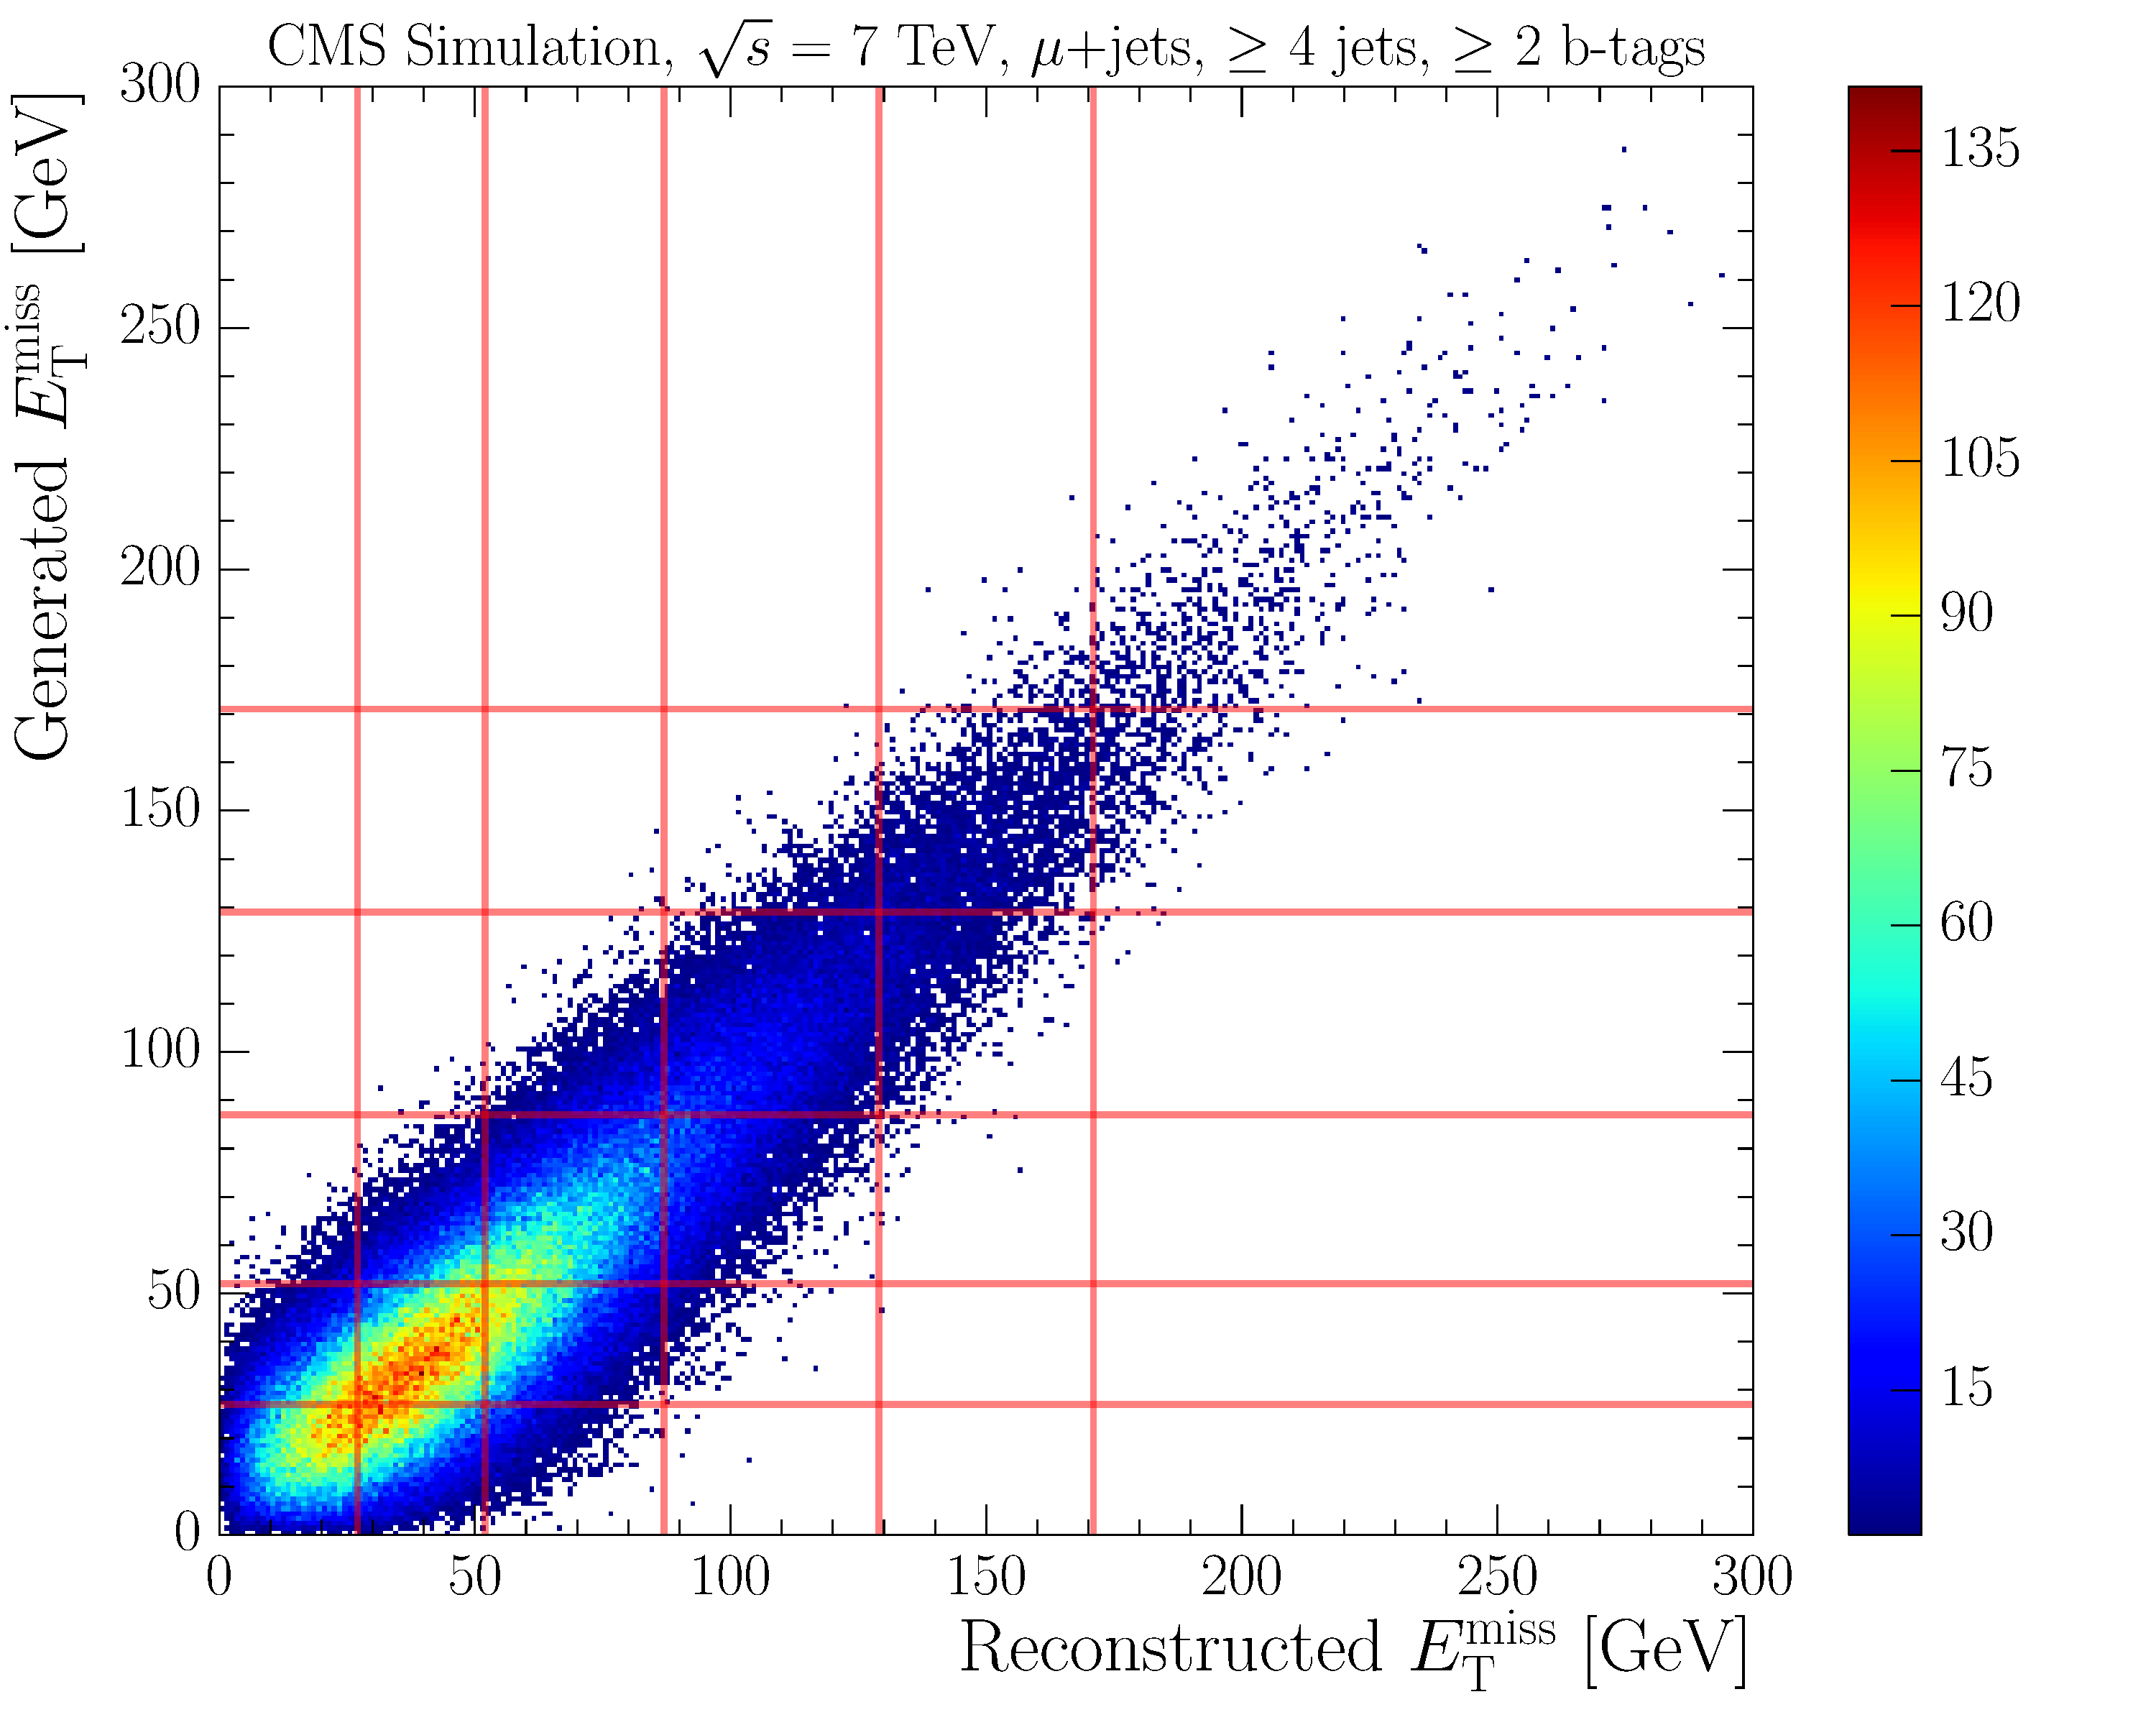
\includegraphics[width=0.48\textwidth]{Chapters/04_Analysis/04b_XSections/images/binning/muon_MET_7TeV.pdf}\hfill
     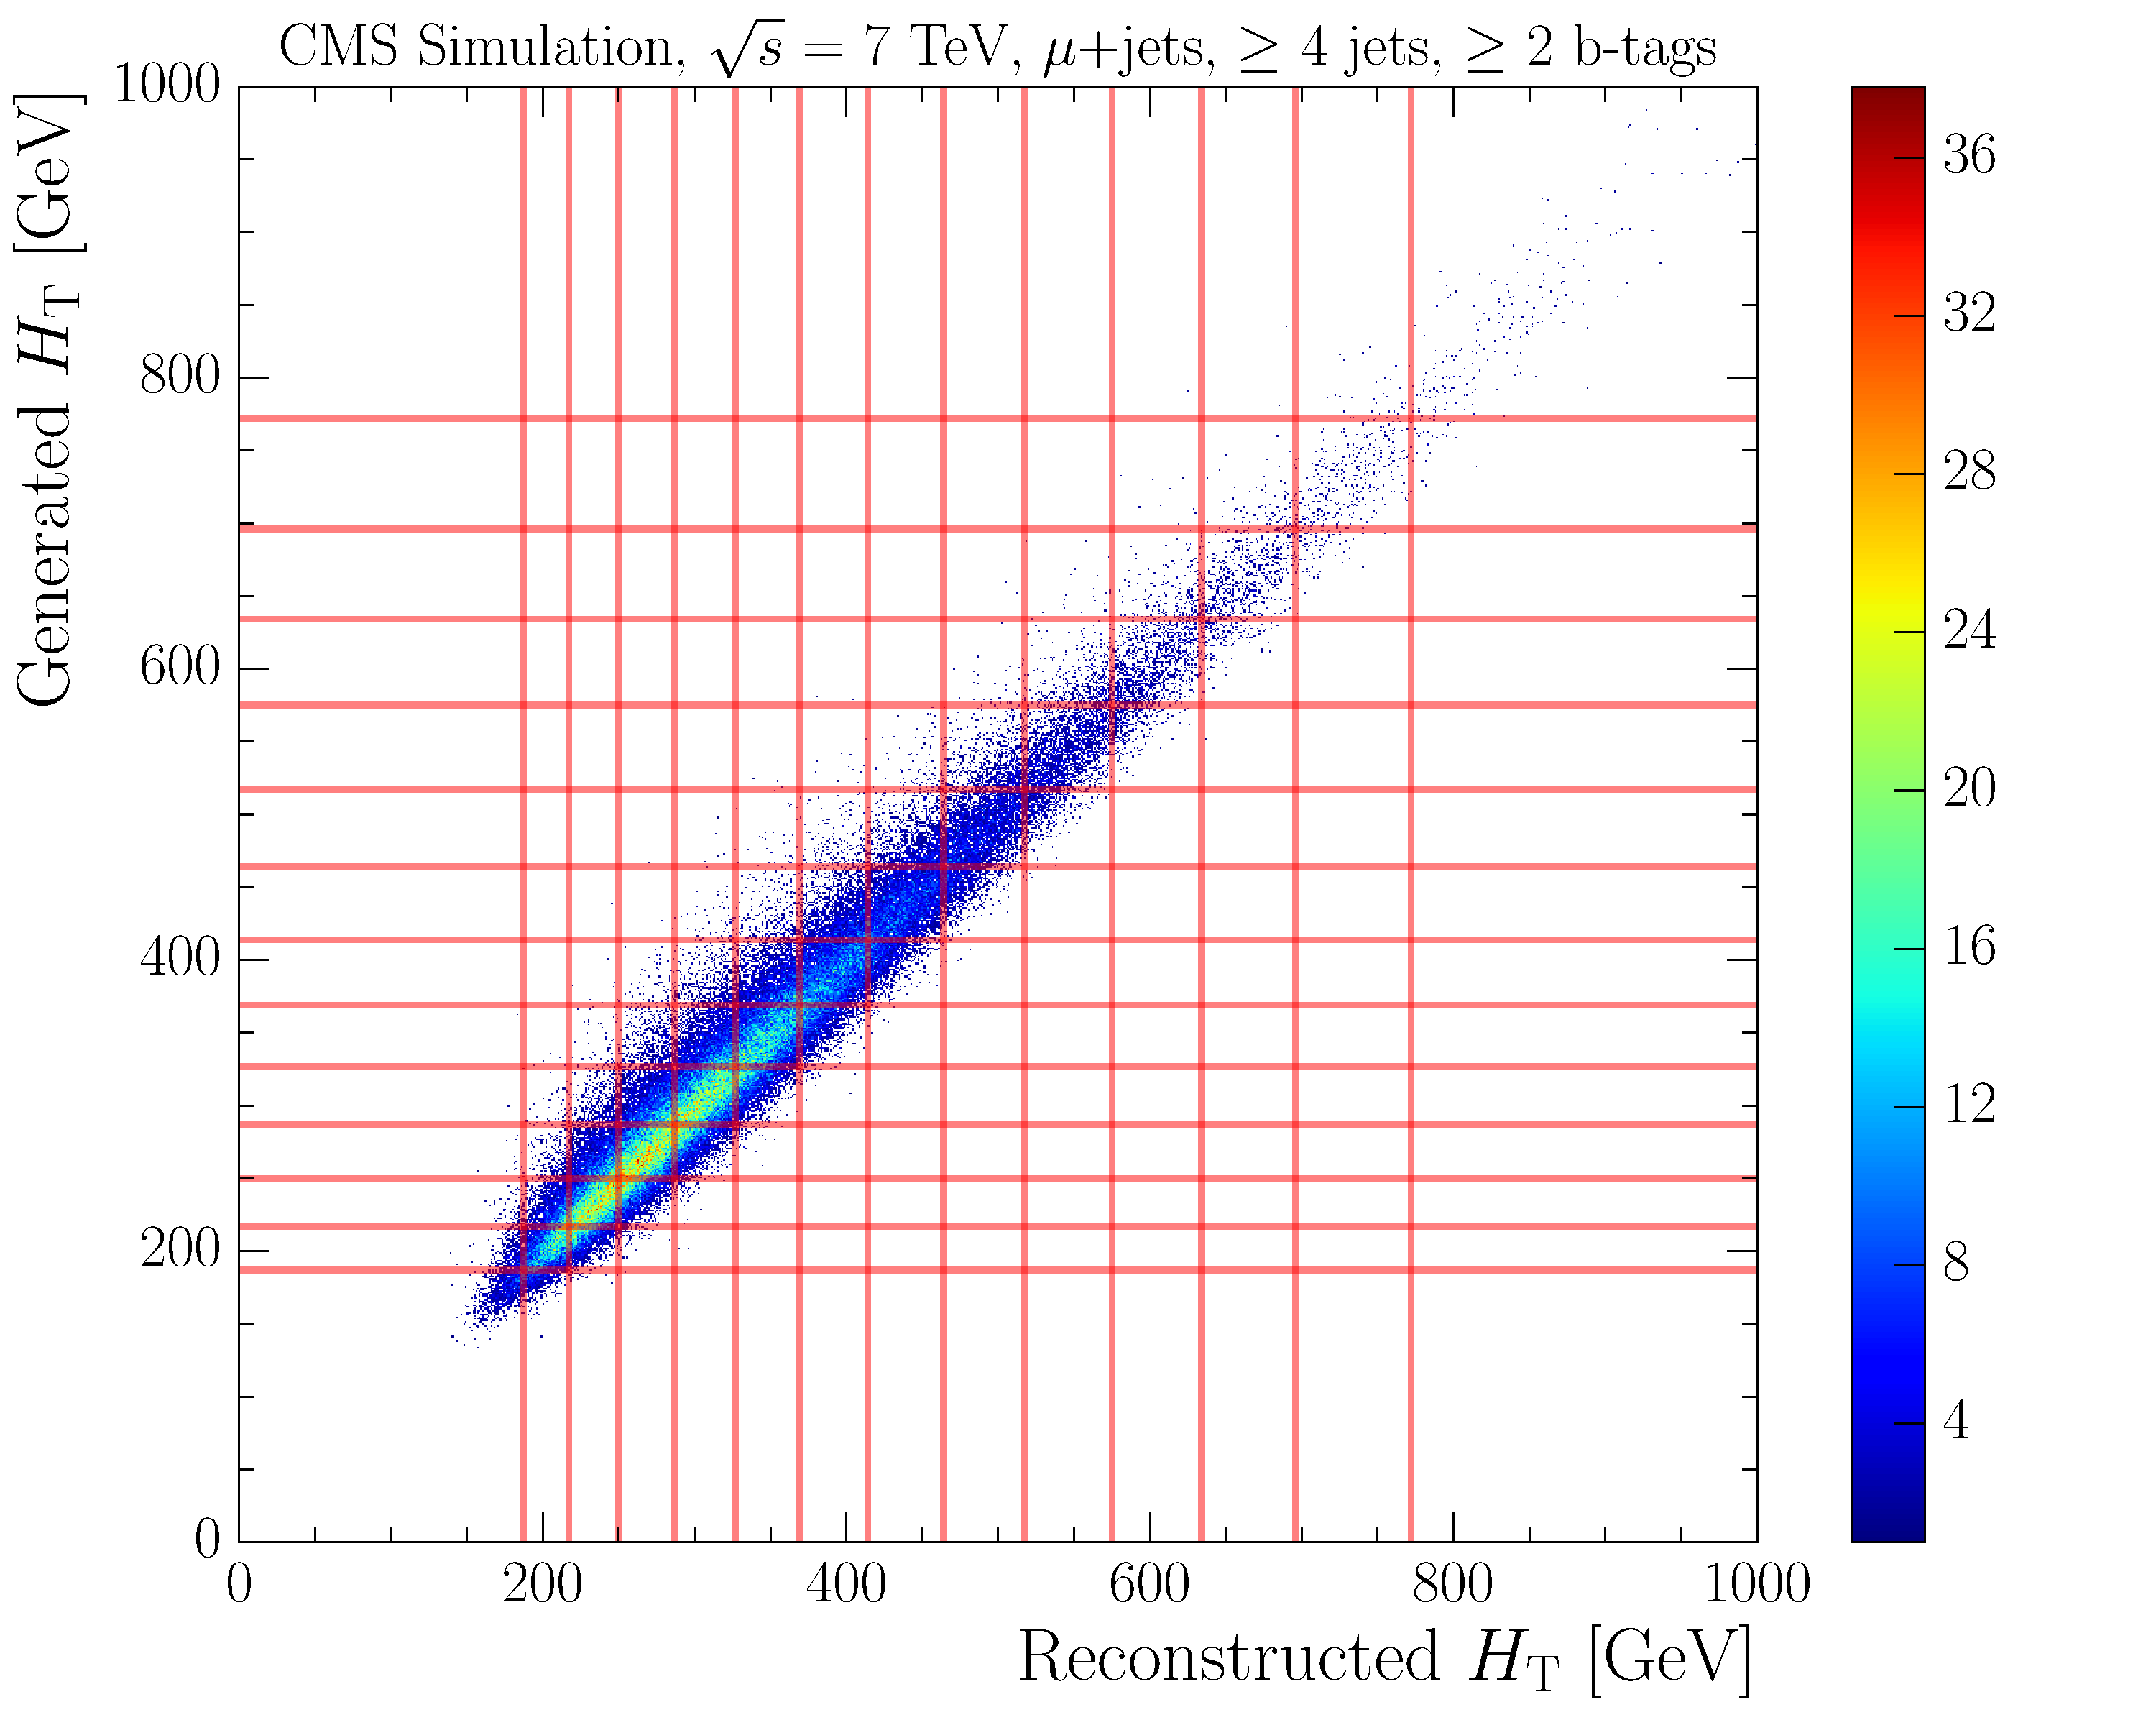
\includegraphics[width=0.48\textwidth]{Chapters/04_Analysis/04b_XSections/images/binning/muon_HT_7TeV.pdf}\\
     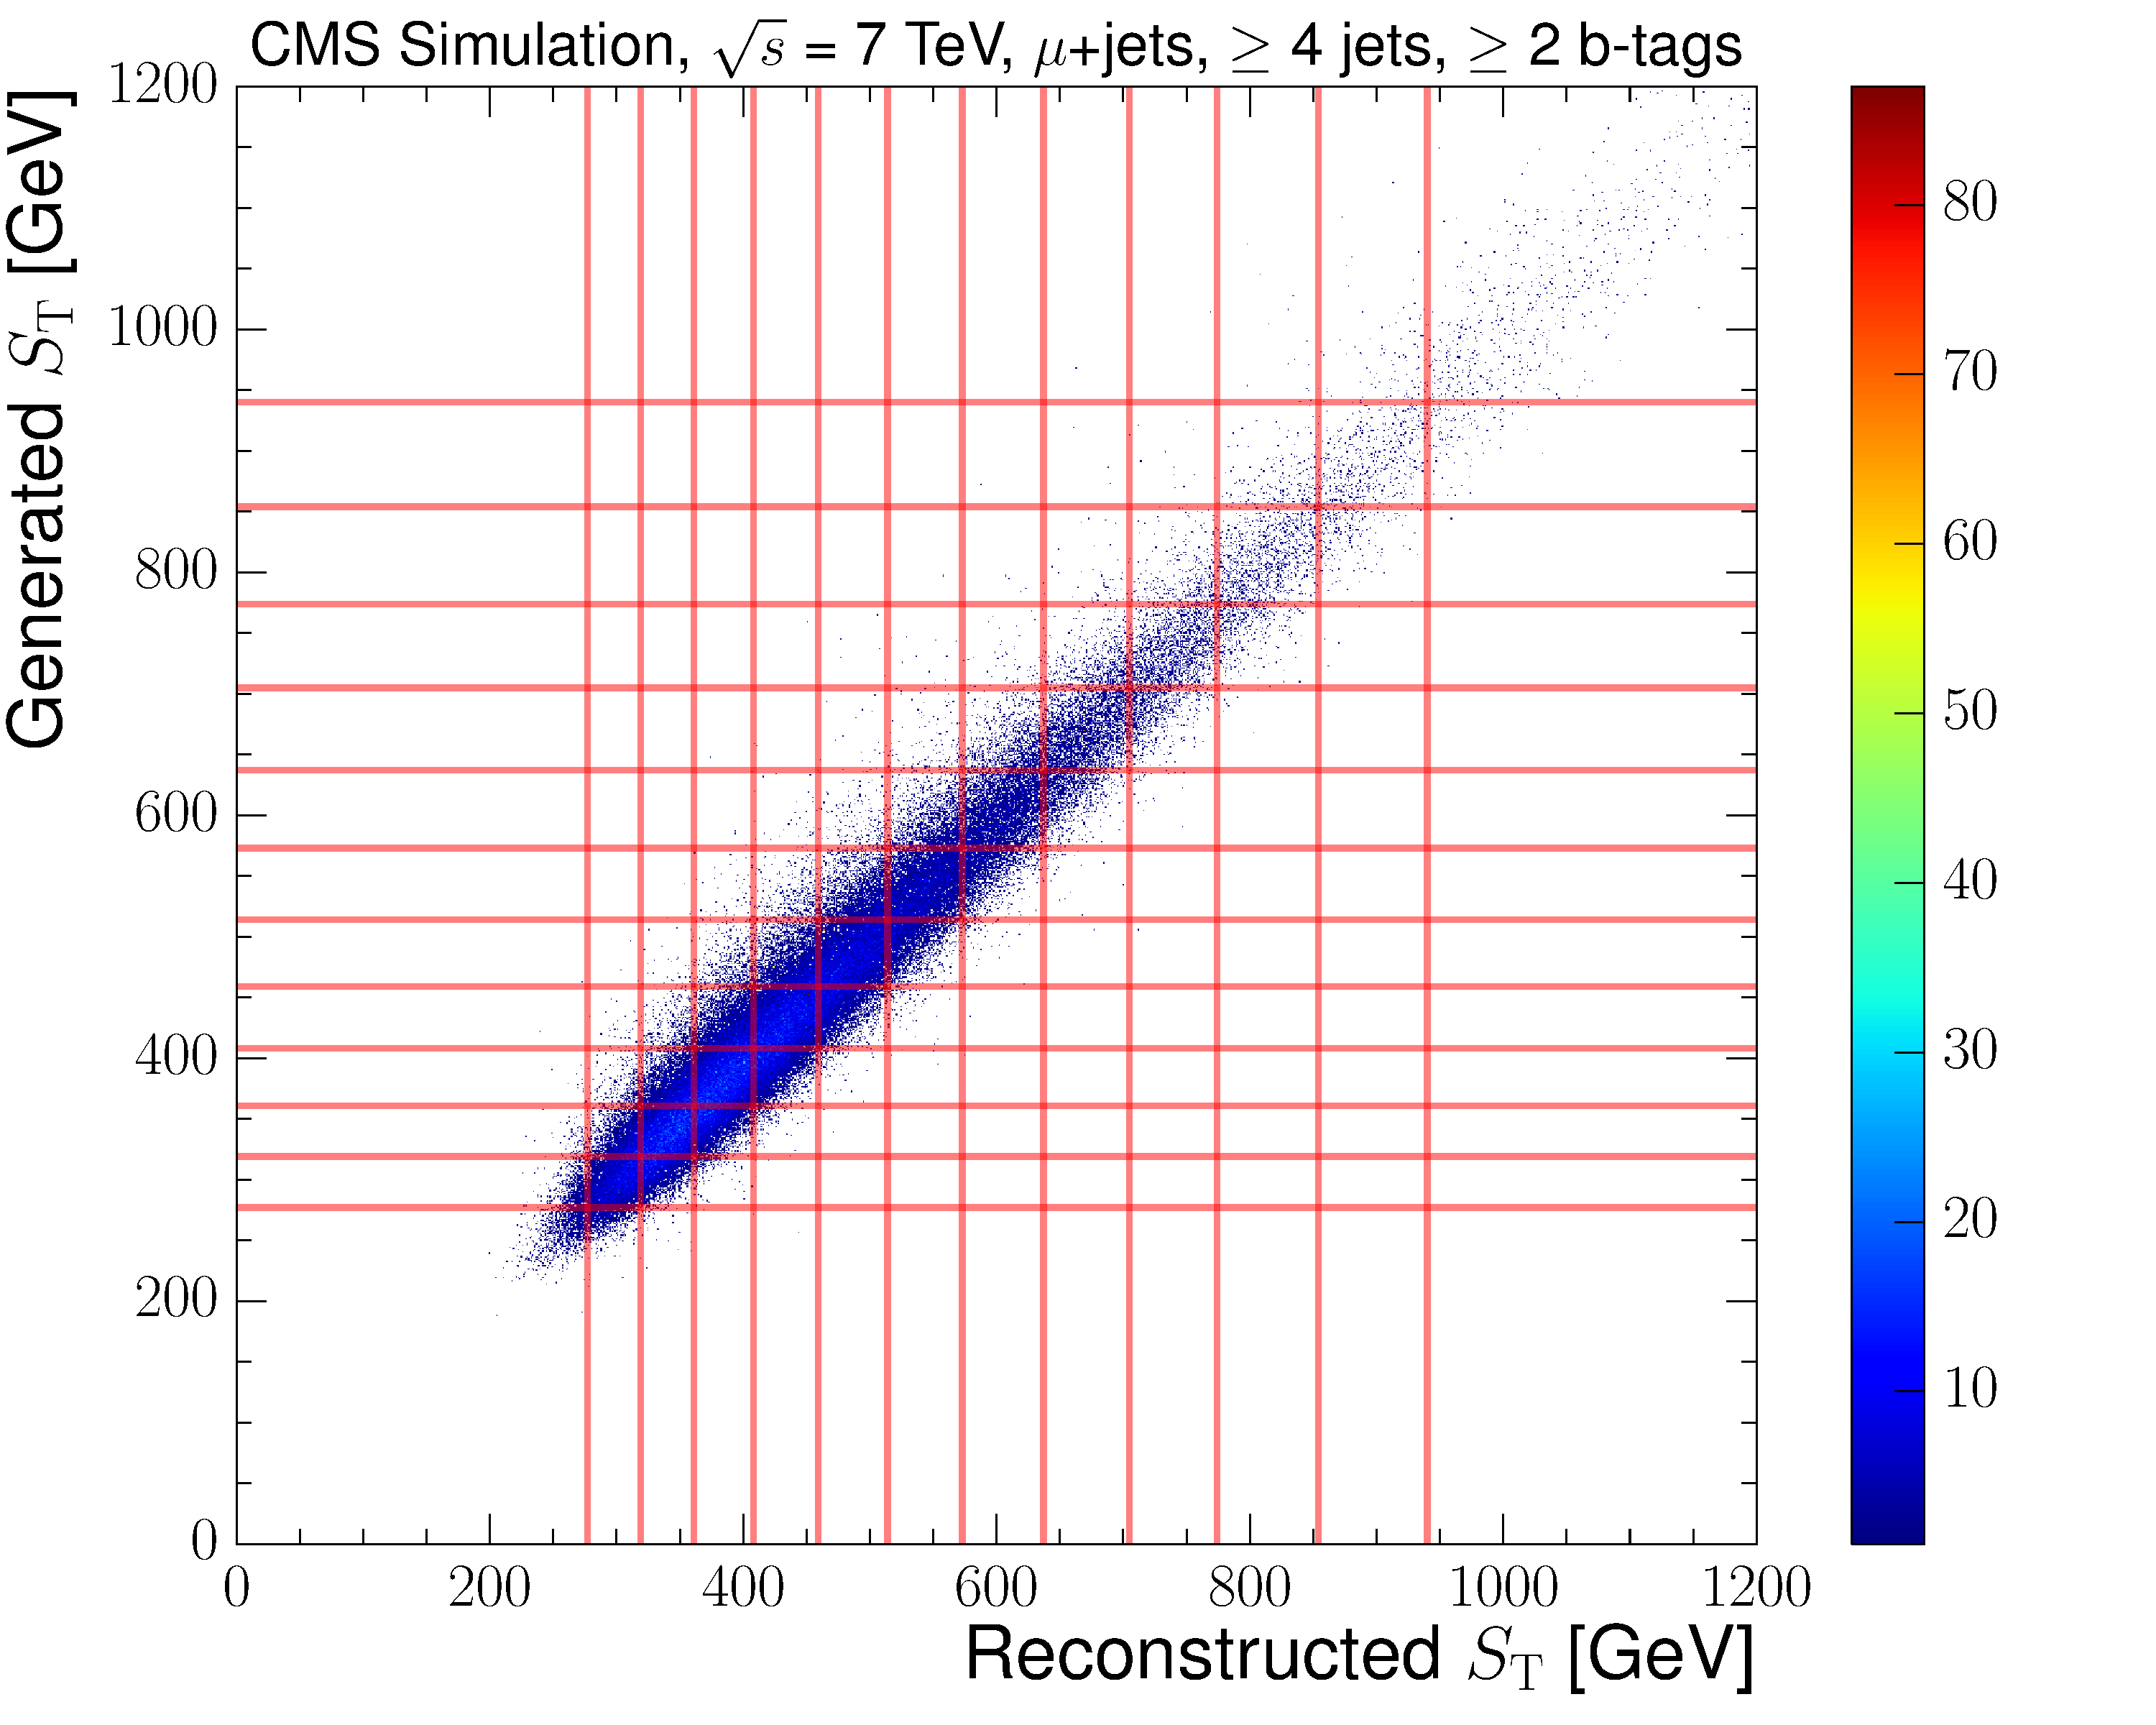
\includegraphics[width=0.48\textwidth]{Chapters/04_Analysis/04b_XSections/images/binning/muon_ST_7TeV.pdf}\hfill
     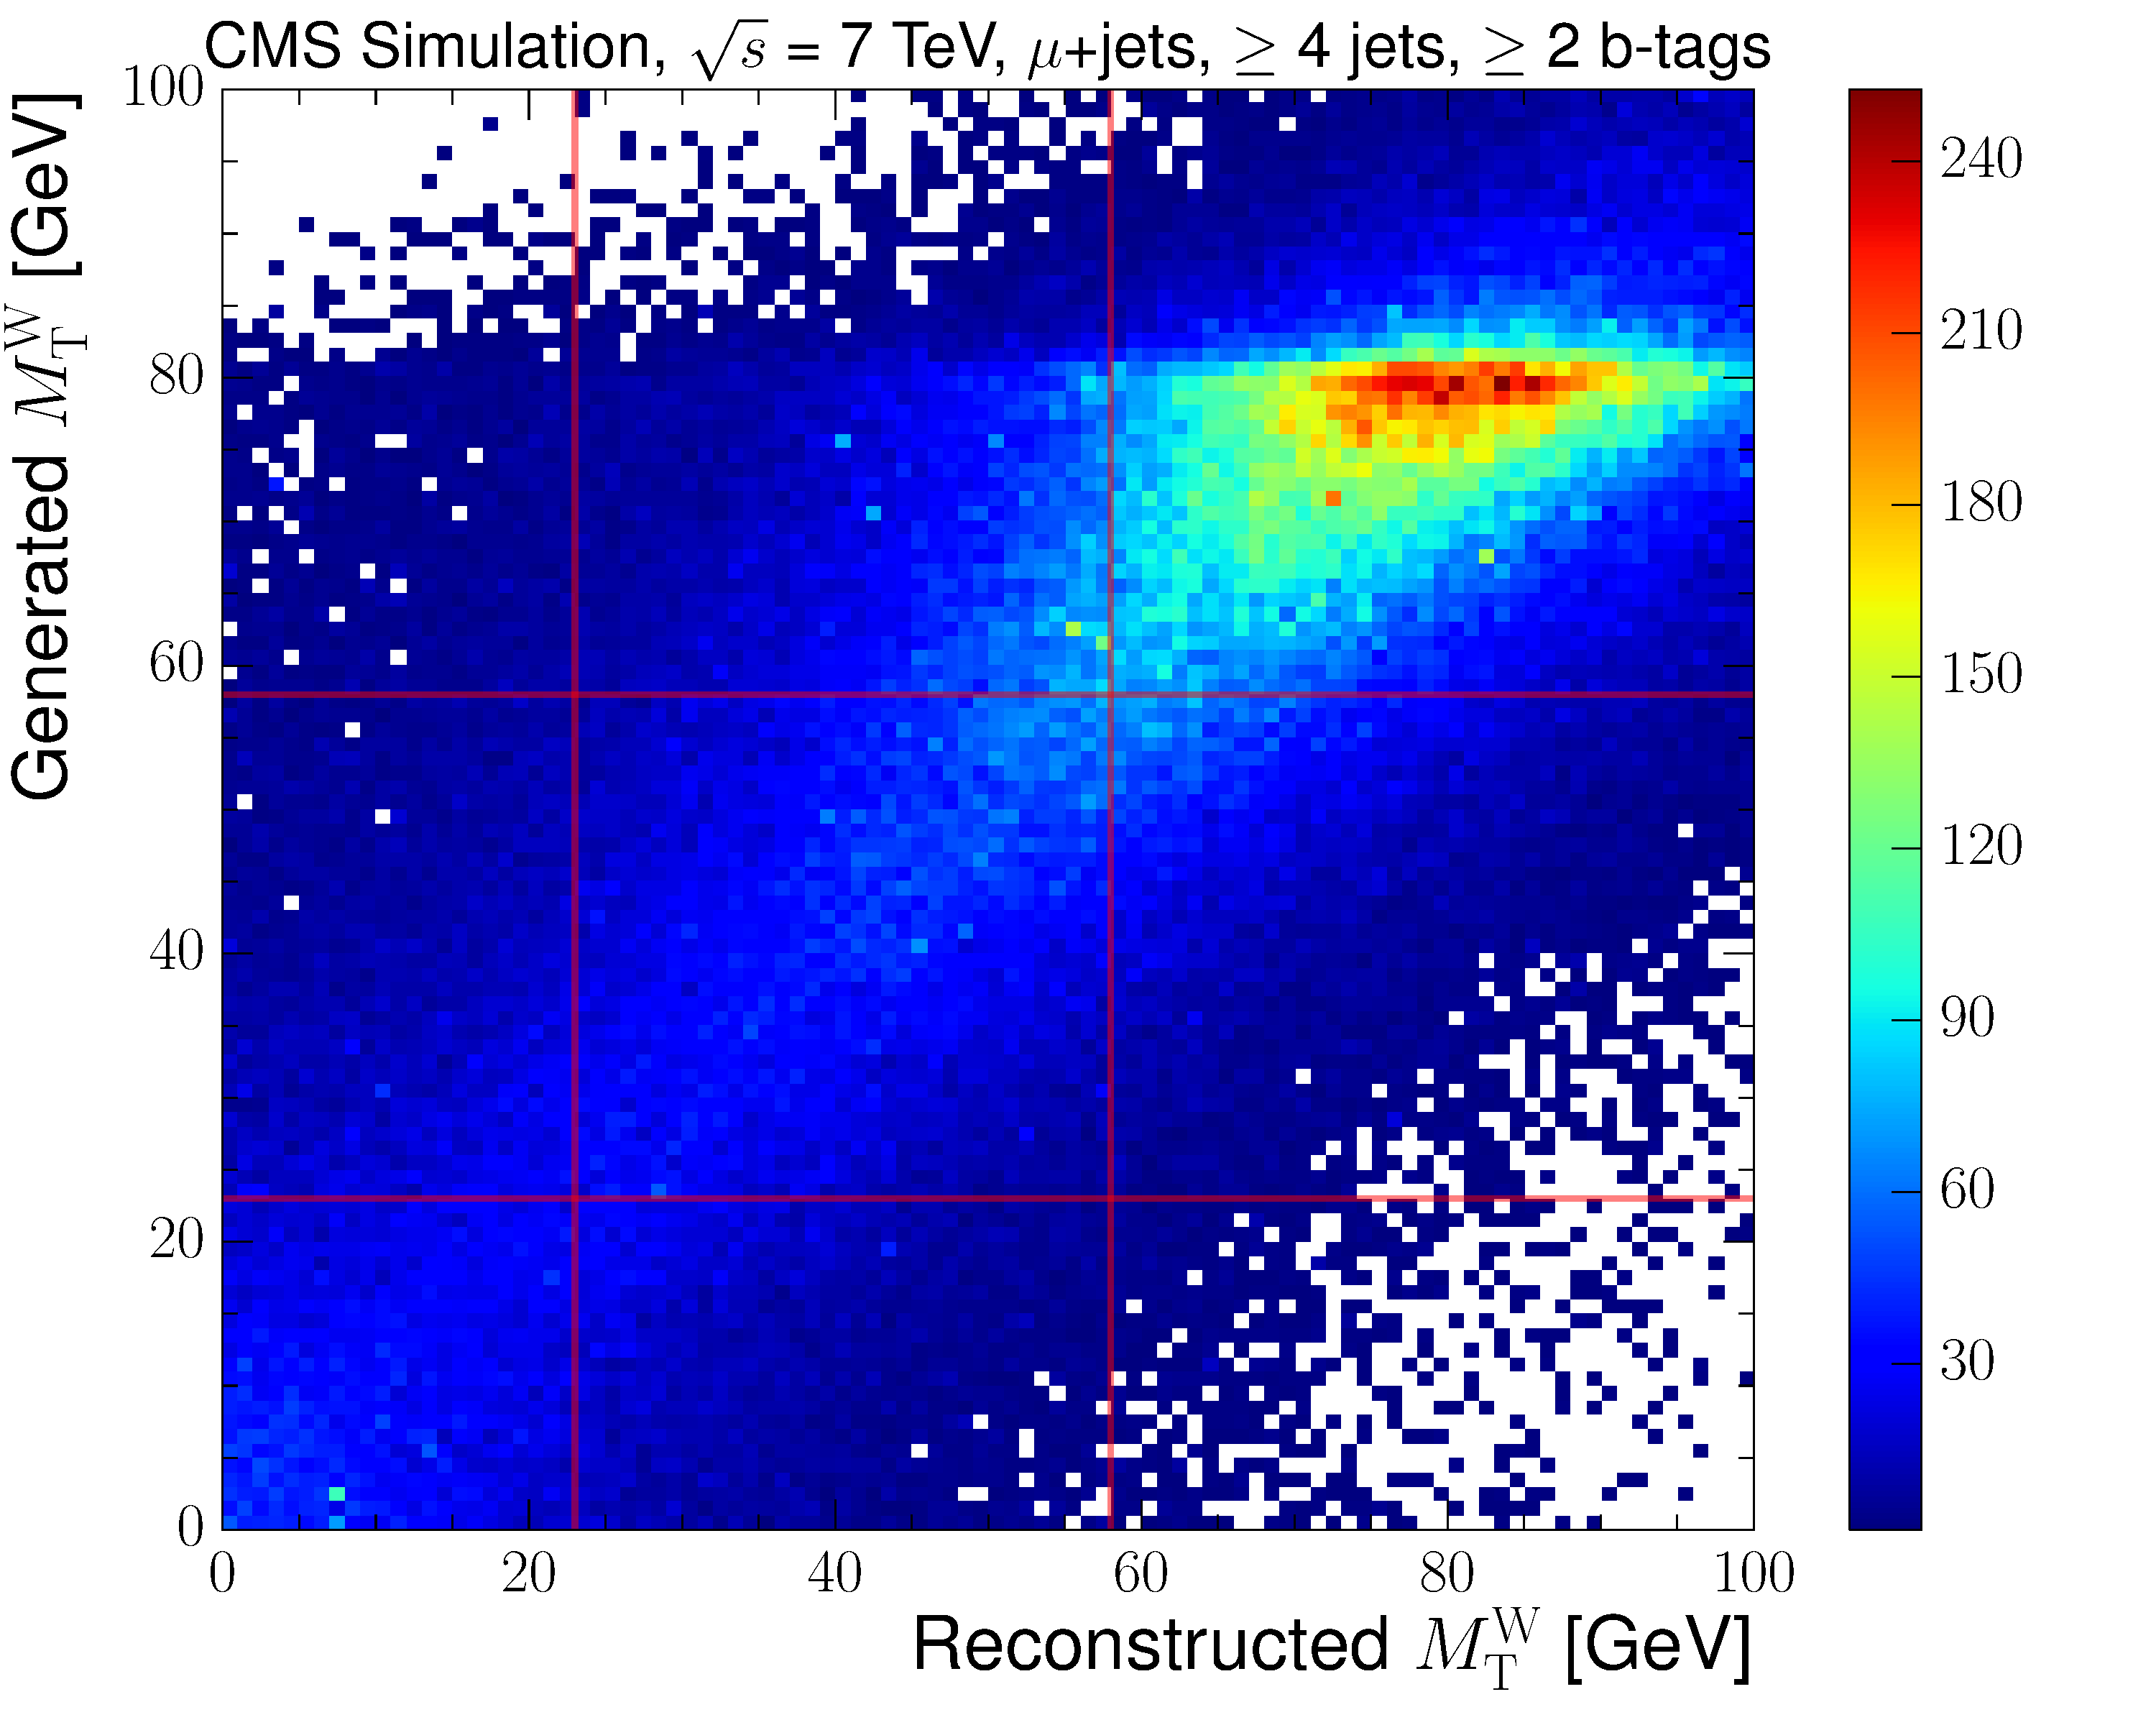
\includegraphics[width=0.48\textwidth]{Chapters/04_Analysis/04b_XSections/images/binning/muon_MT_7TeV.pdf}\\
	 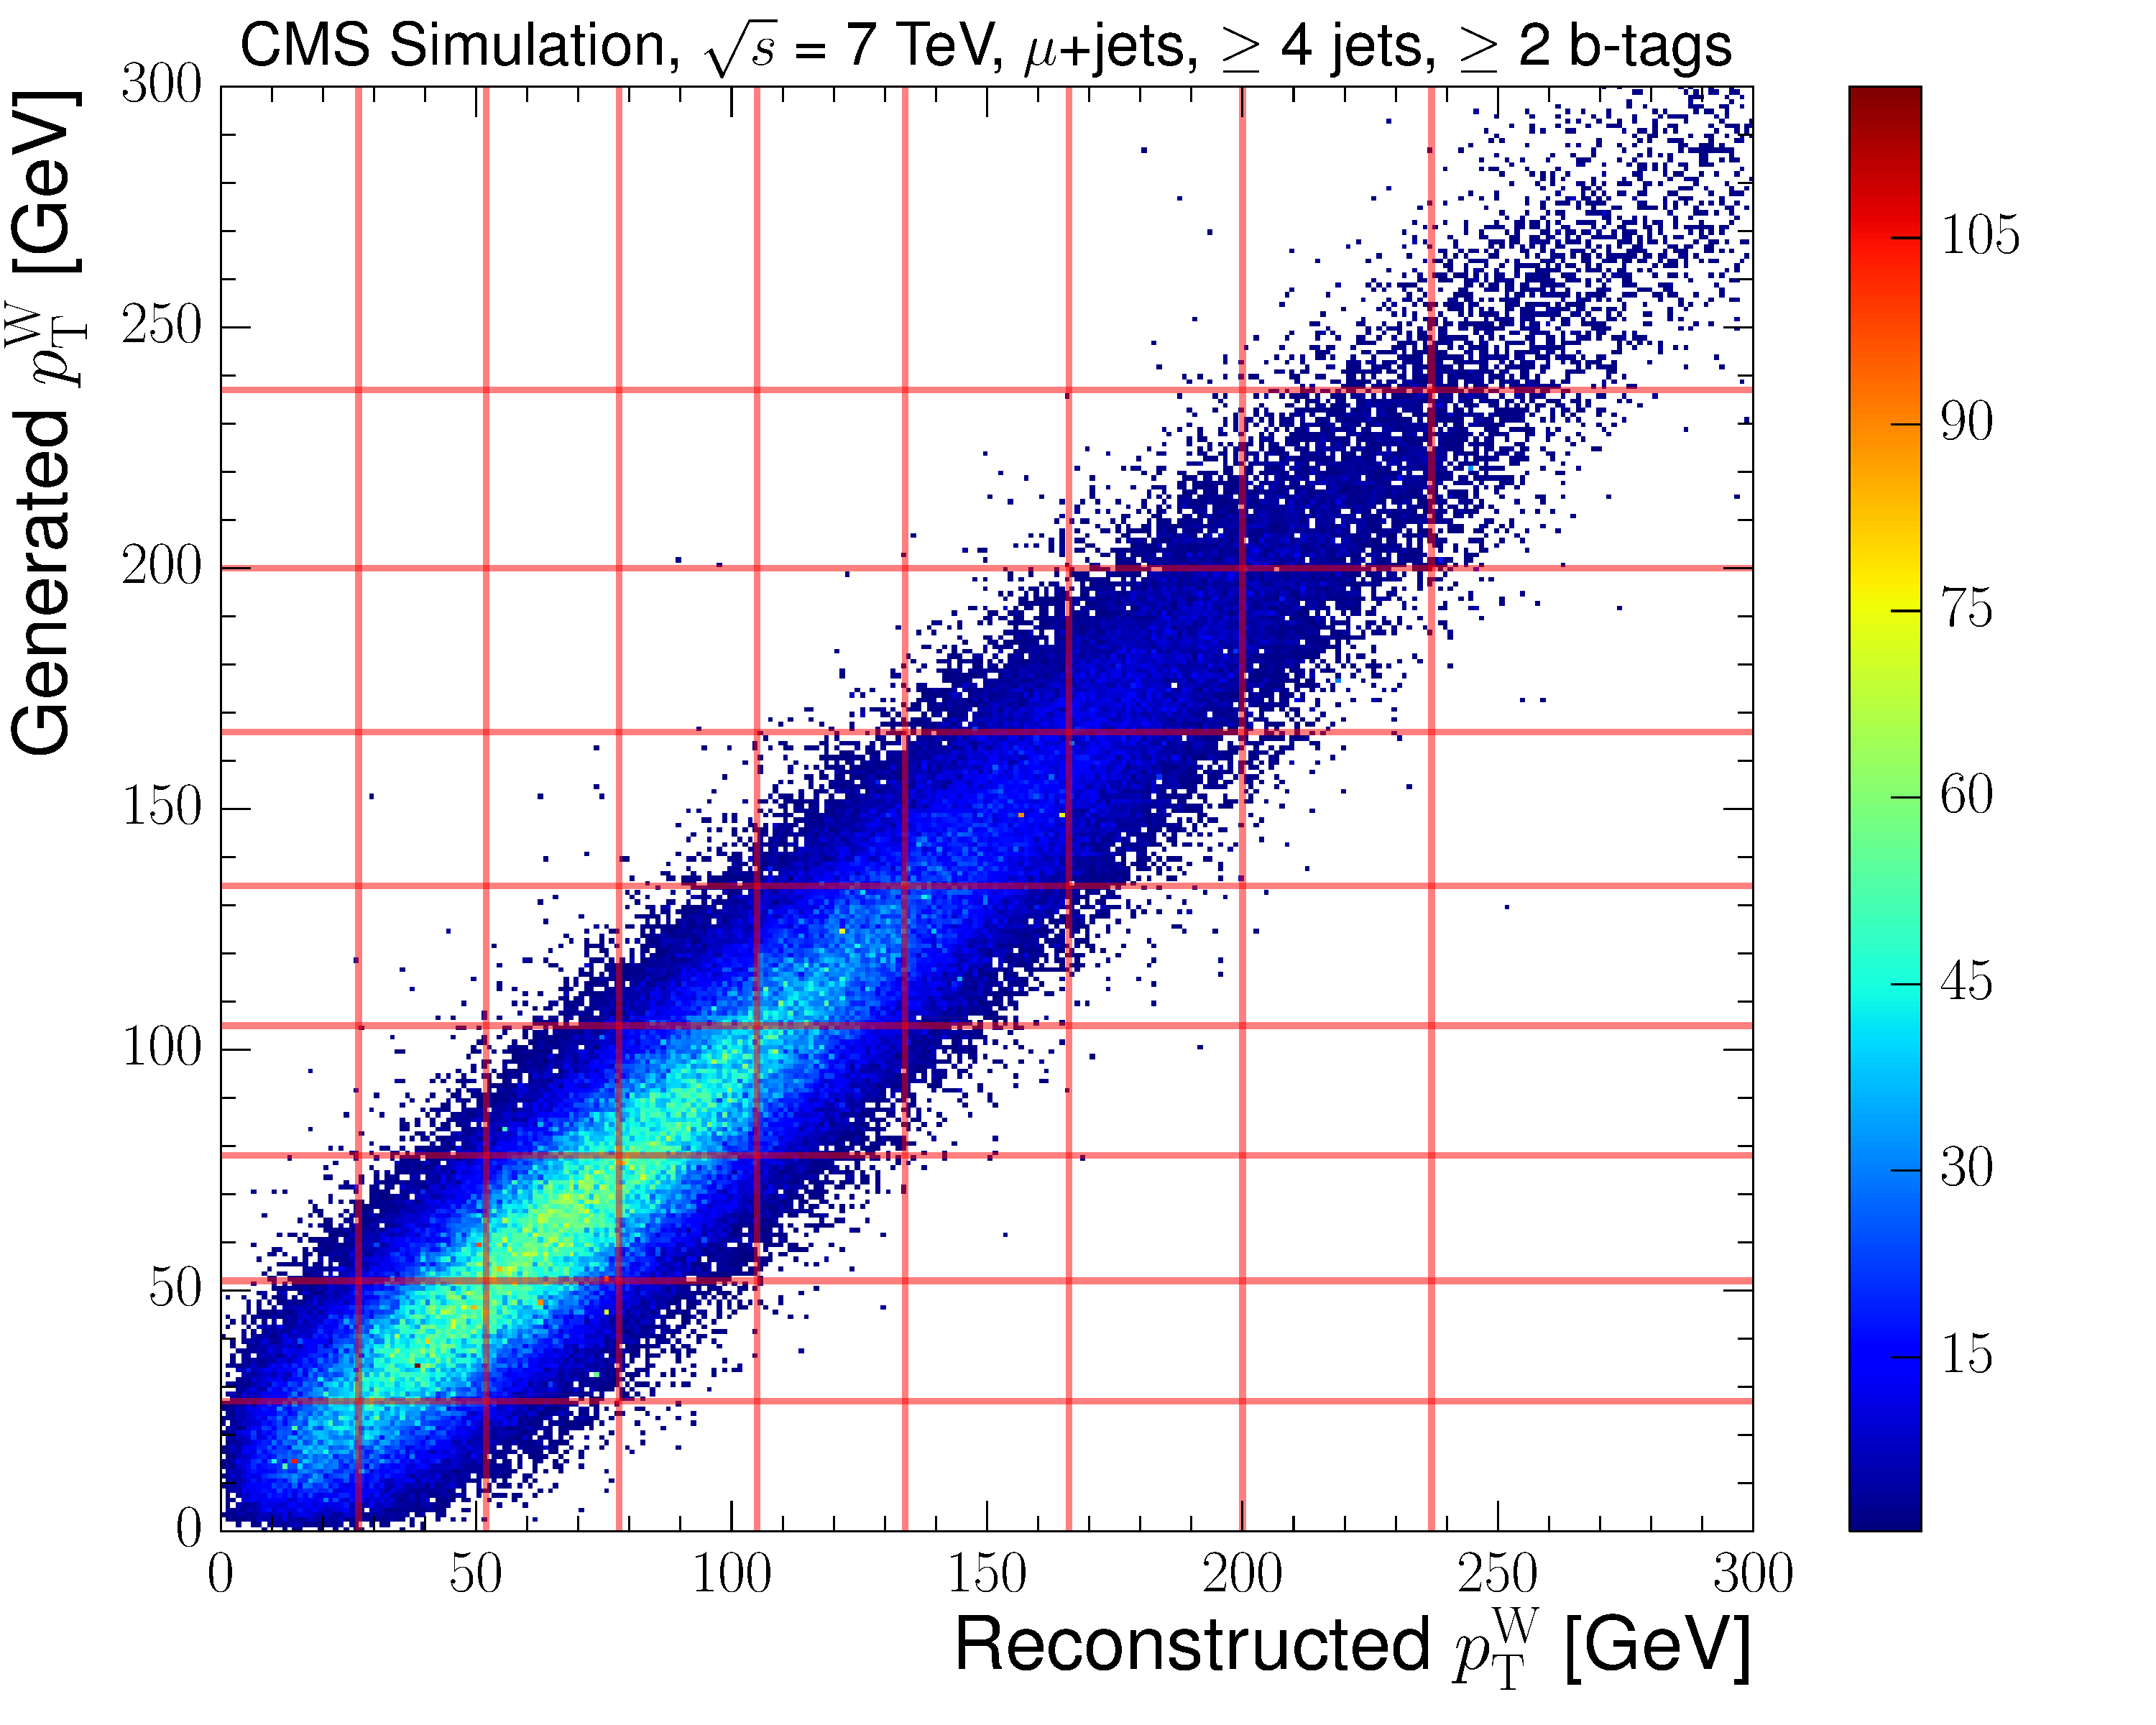
\includegraphics[width=0.48\textwidth]{Chapters/04_Analysis/04b_XSections/images/binning/muon_WPT_7TeV.pdf}\hfill
	 \caption{Generated versus reconstructed distributions of the primary variables \met (upper left), \HT (upper
	 right), \st (middle left), \mt (middle right) and \wpt (lower) with horizontal and vertical lines
	 representing the boundaries of the selected bins at $\sqrt{s}=7\TeV$ in the muon+jets channel. These
	 distributions are obtained using \ttbar Monte Carlo simulation.}
     \label{fig:binning_7TeV_muon}
 \end{figure}

 \begin{figure}[hbtp]
    \centering
     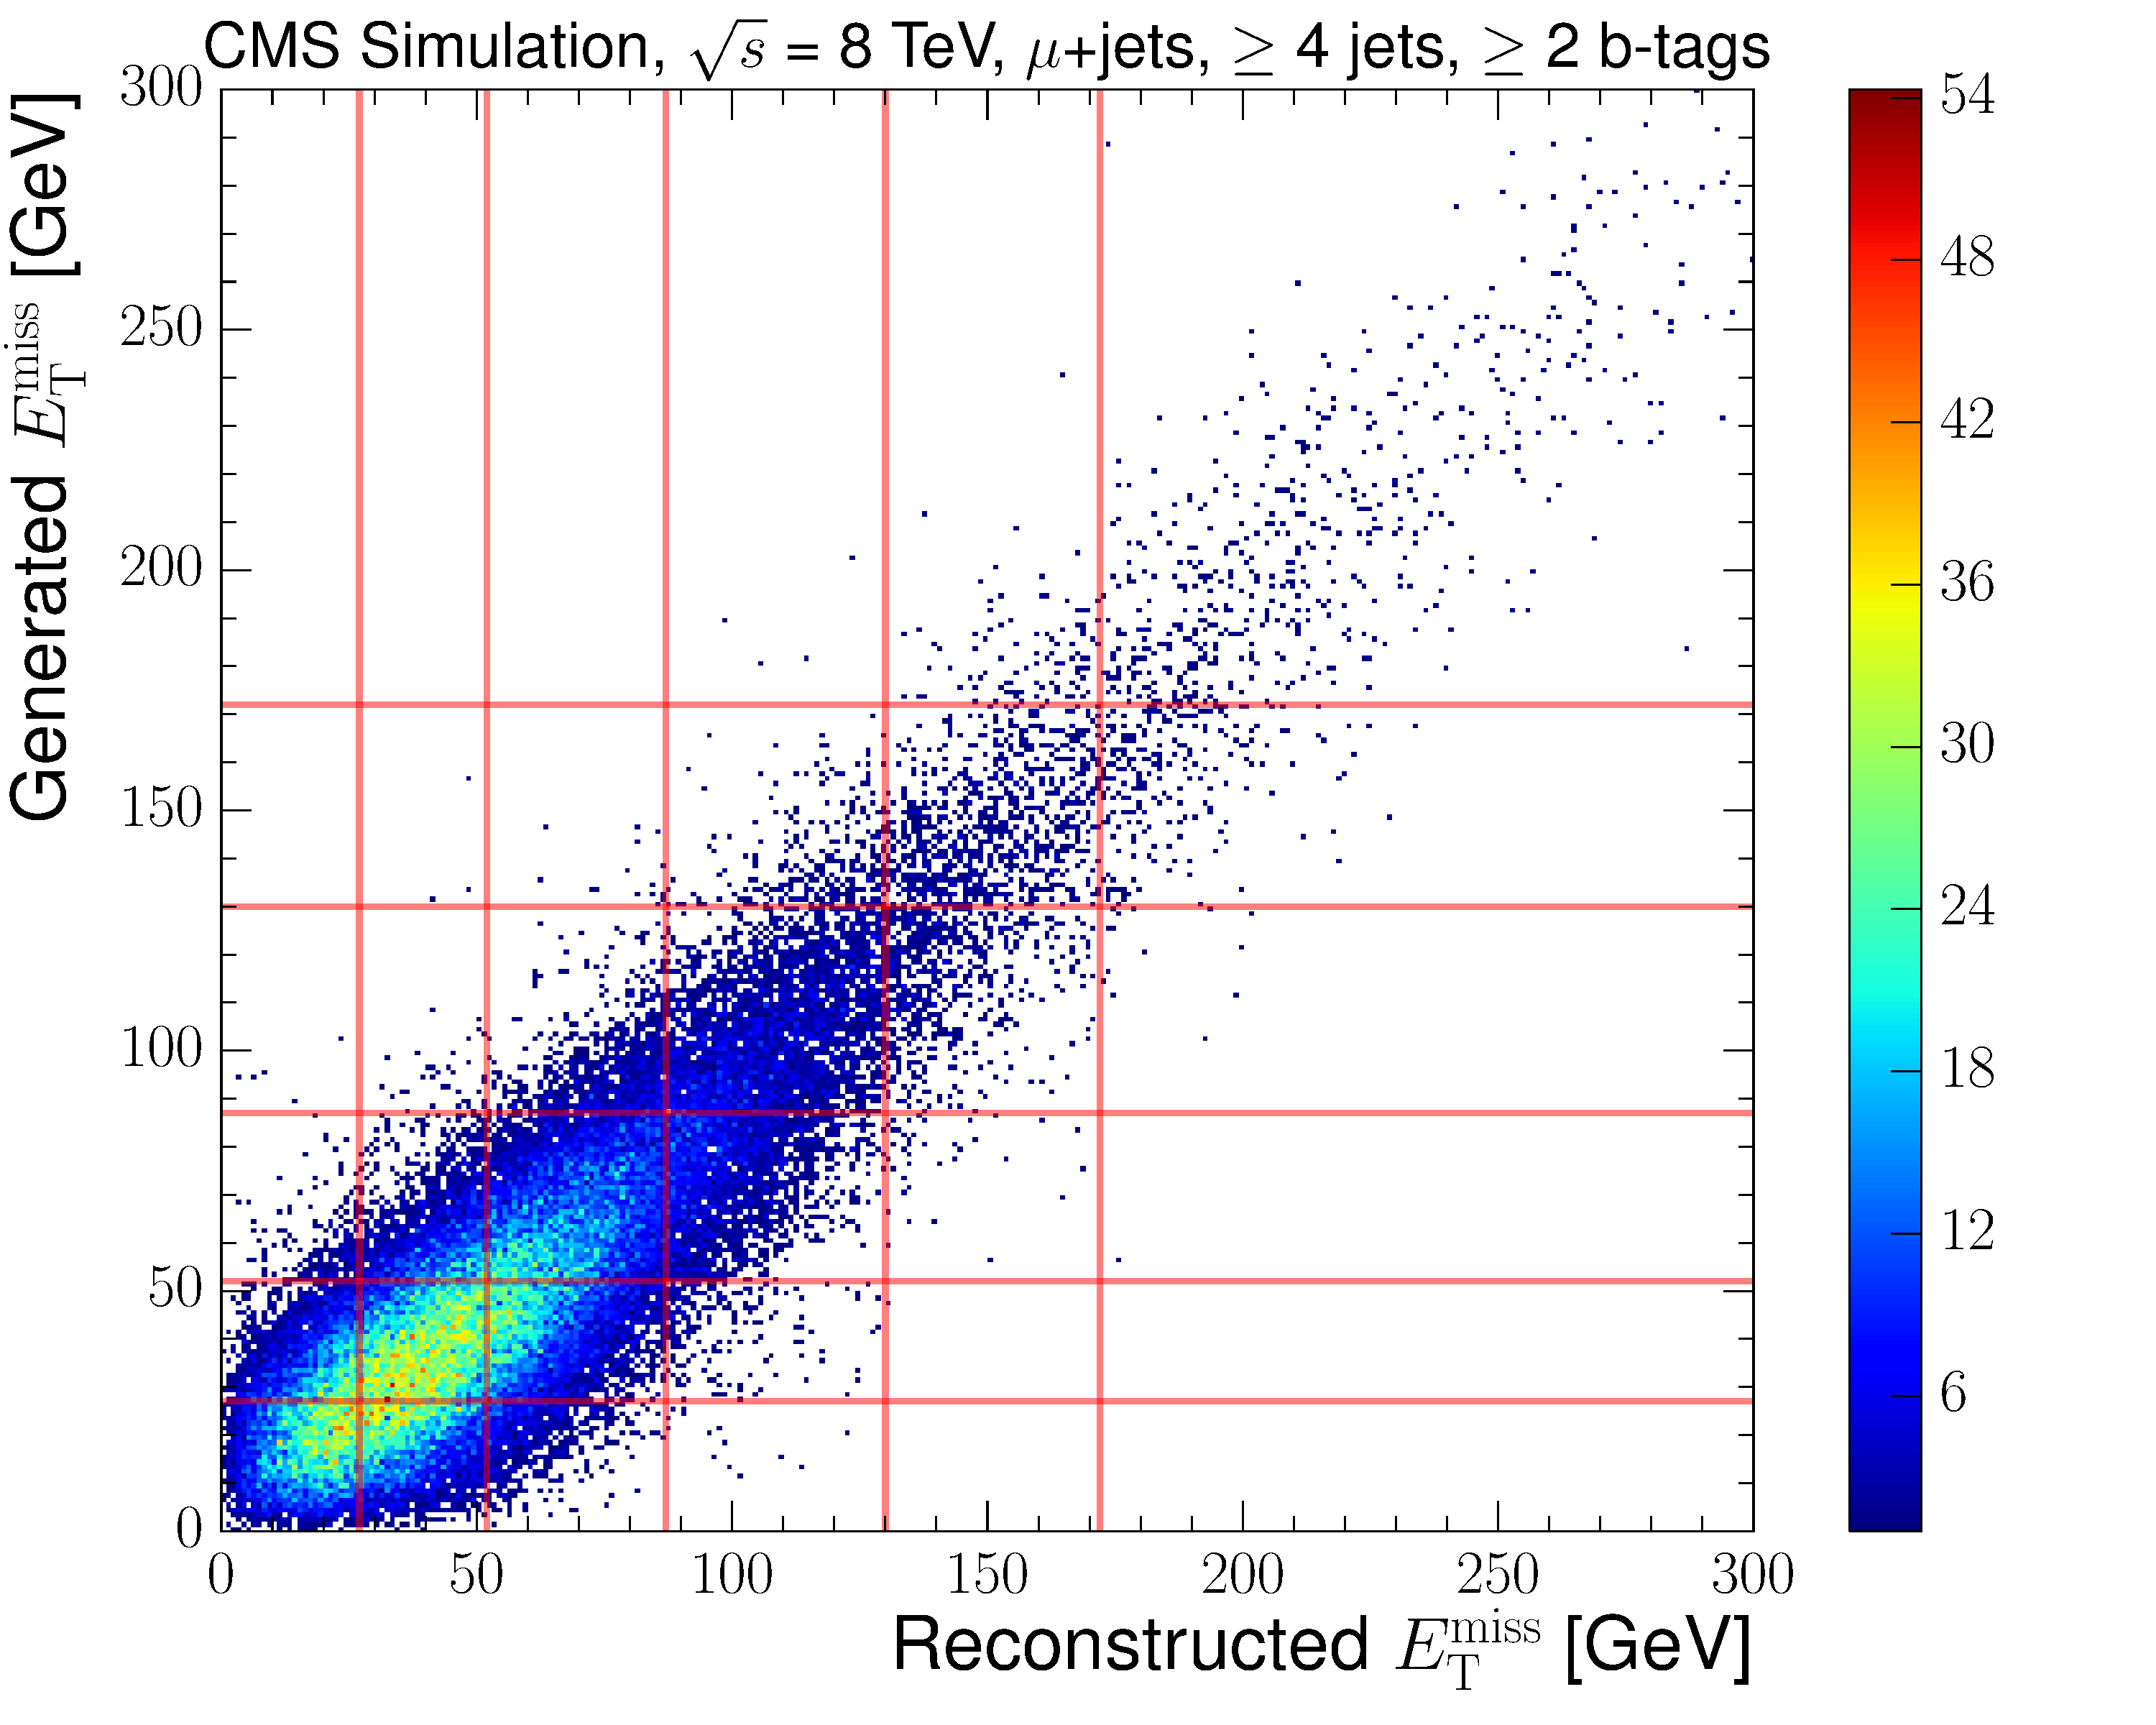
\includegraphics[width=0.48\textwidth]{Chapters/04_Analysis/04b_XSections/images/binning/muon_MET_8TeV.pdf}\hfill
     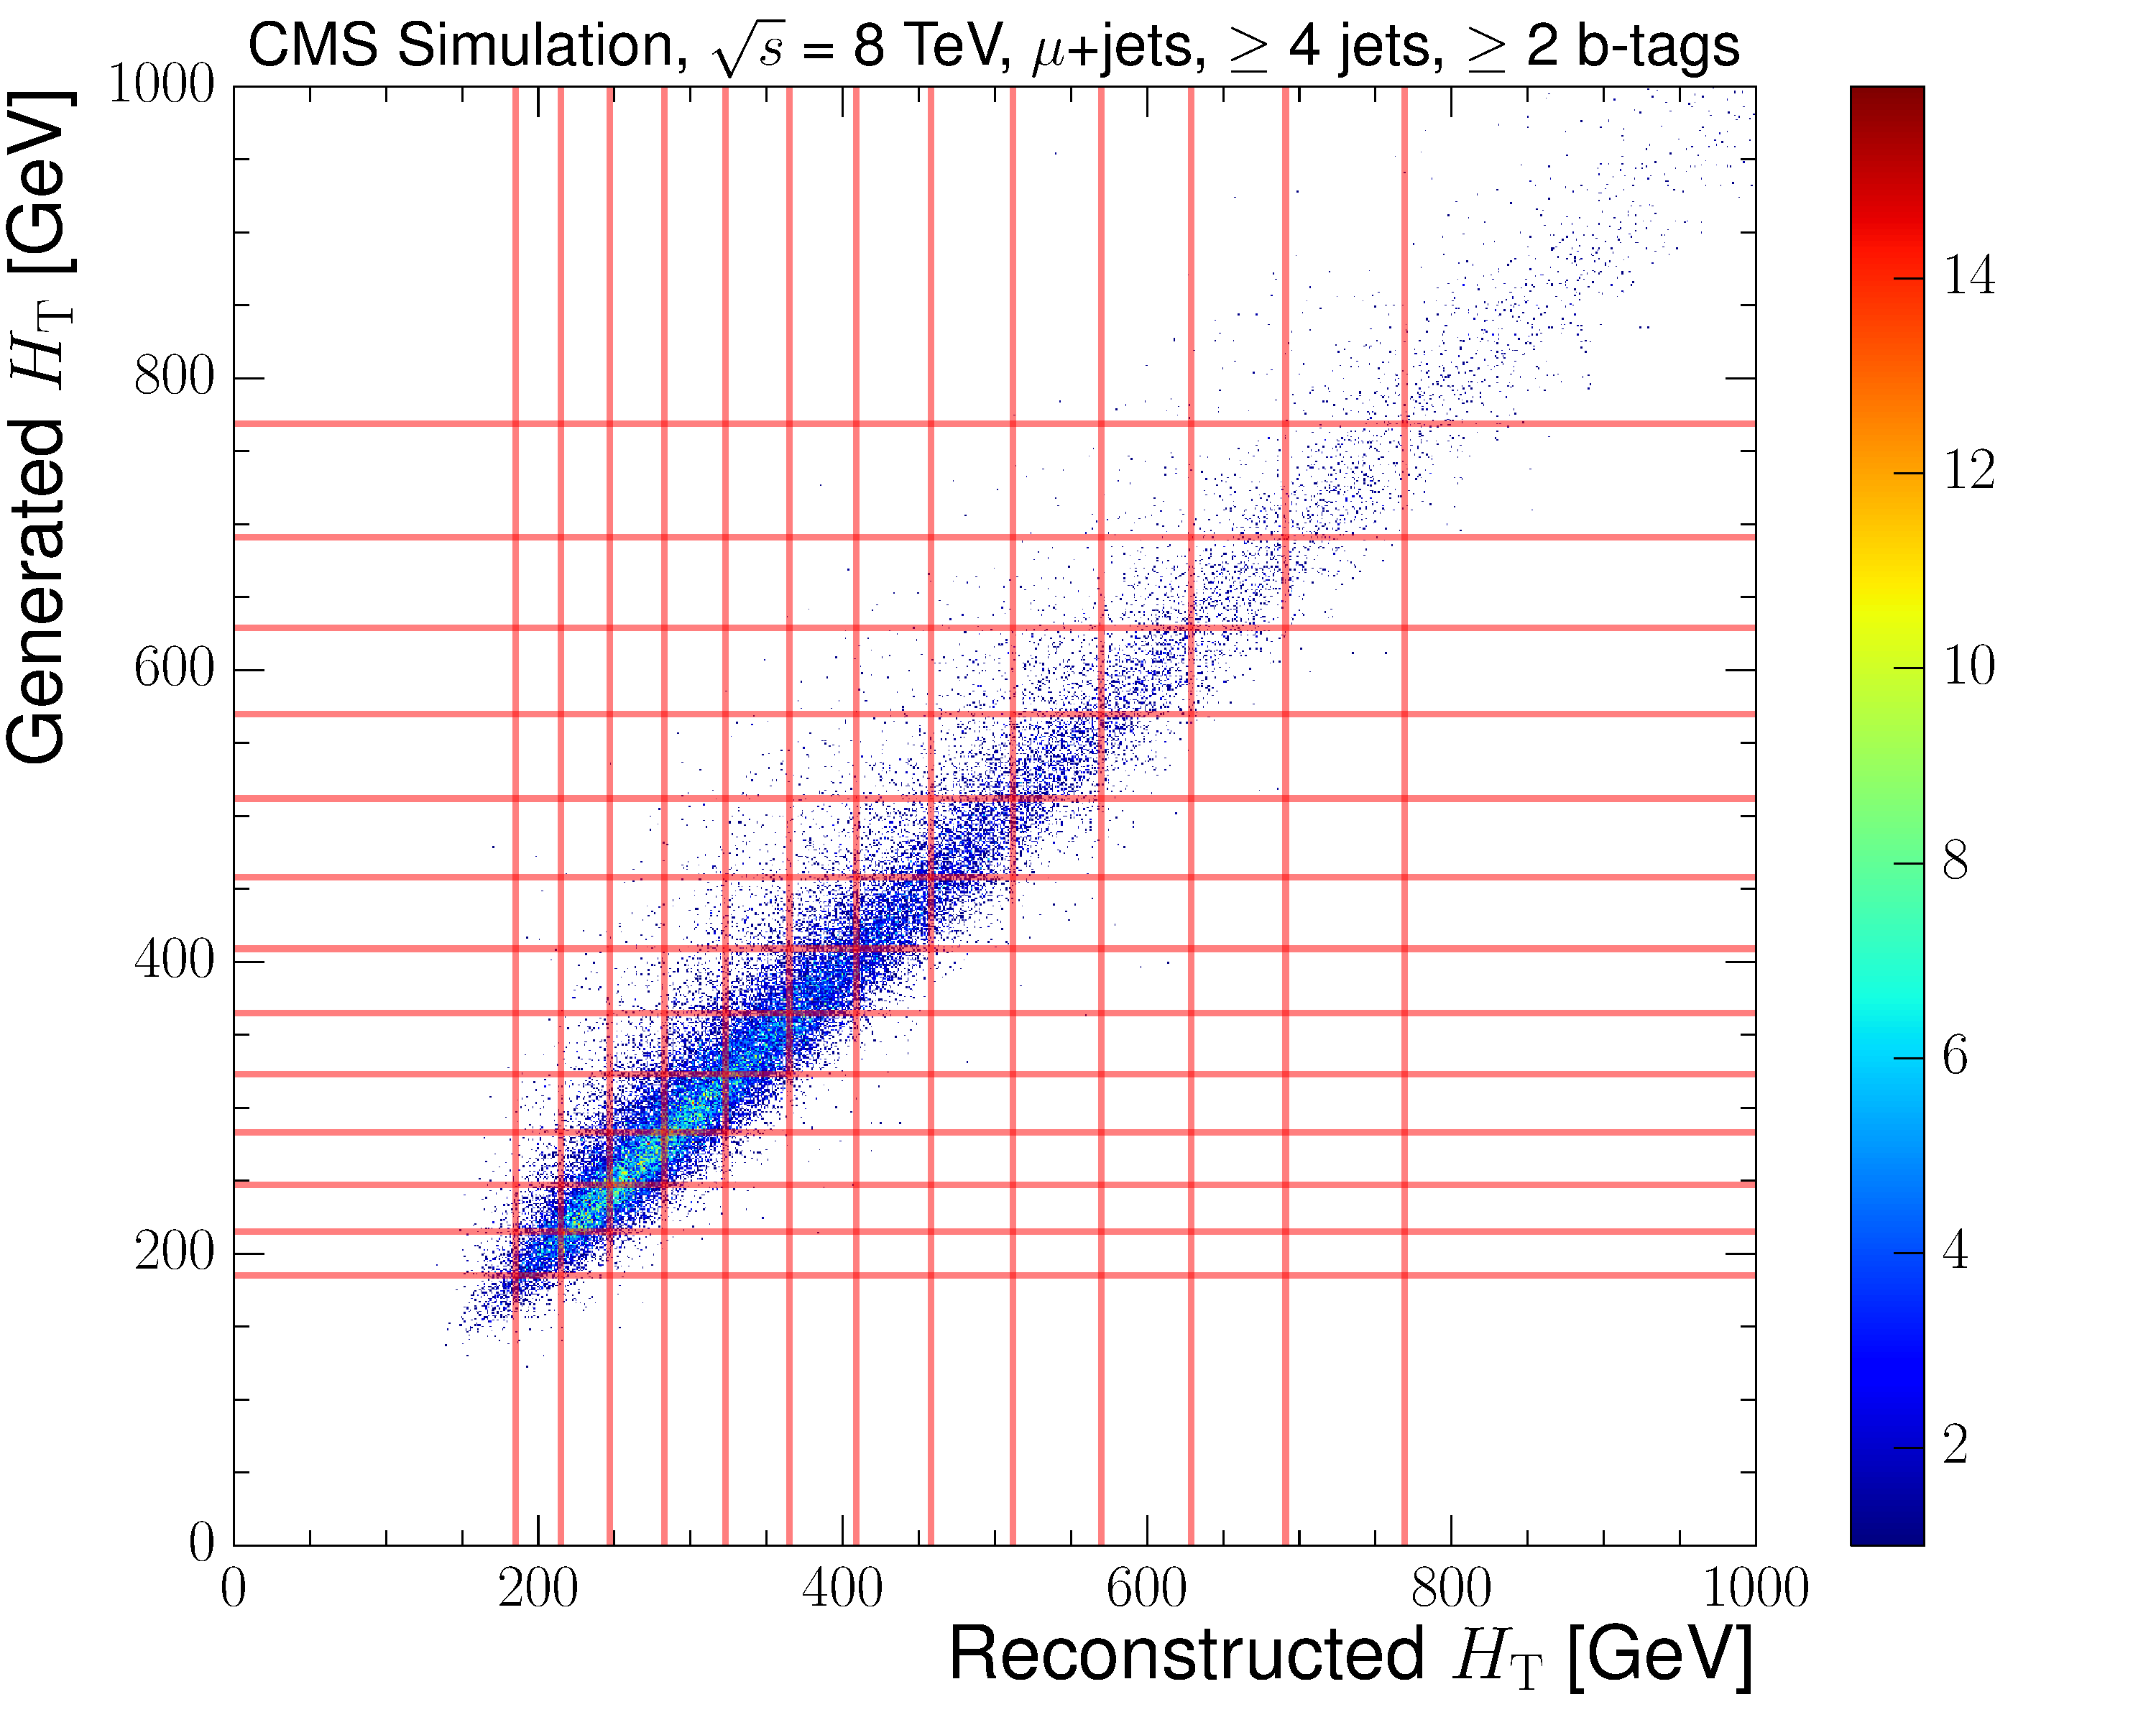
\includegraphics[width=0.48\textwidth]{Chapters/04_Analysis/04b_XSections/images/binning/muon_HT_8TeV.pdf}\\
     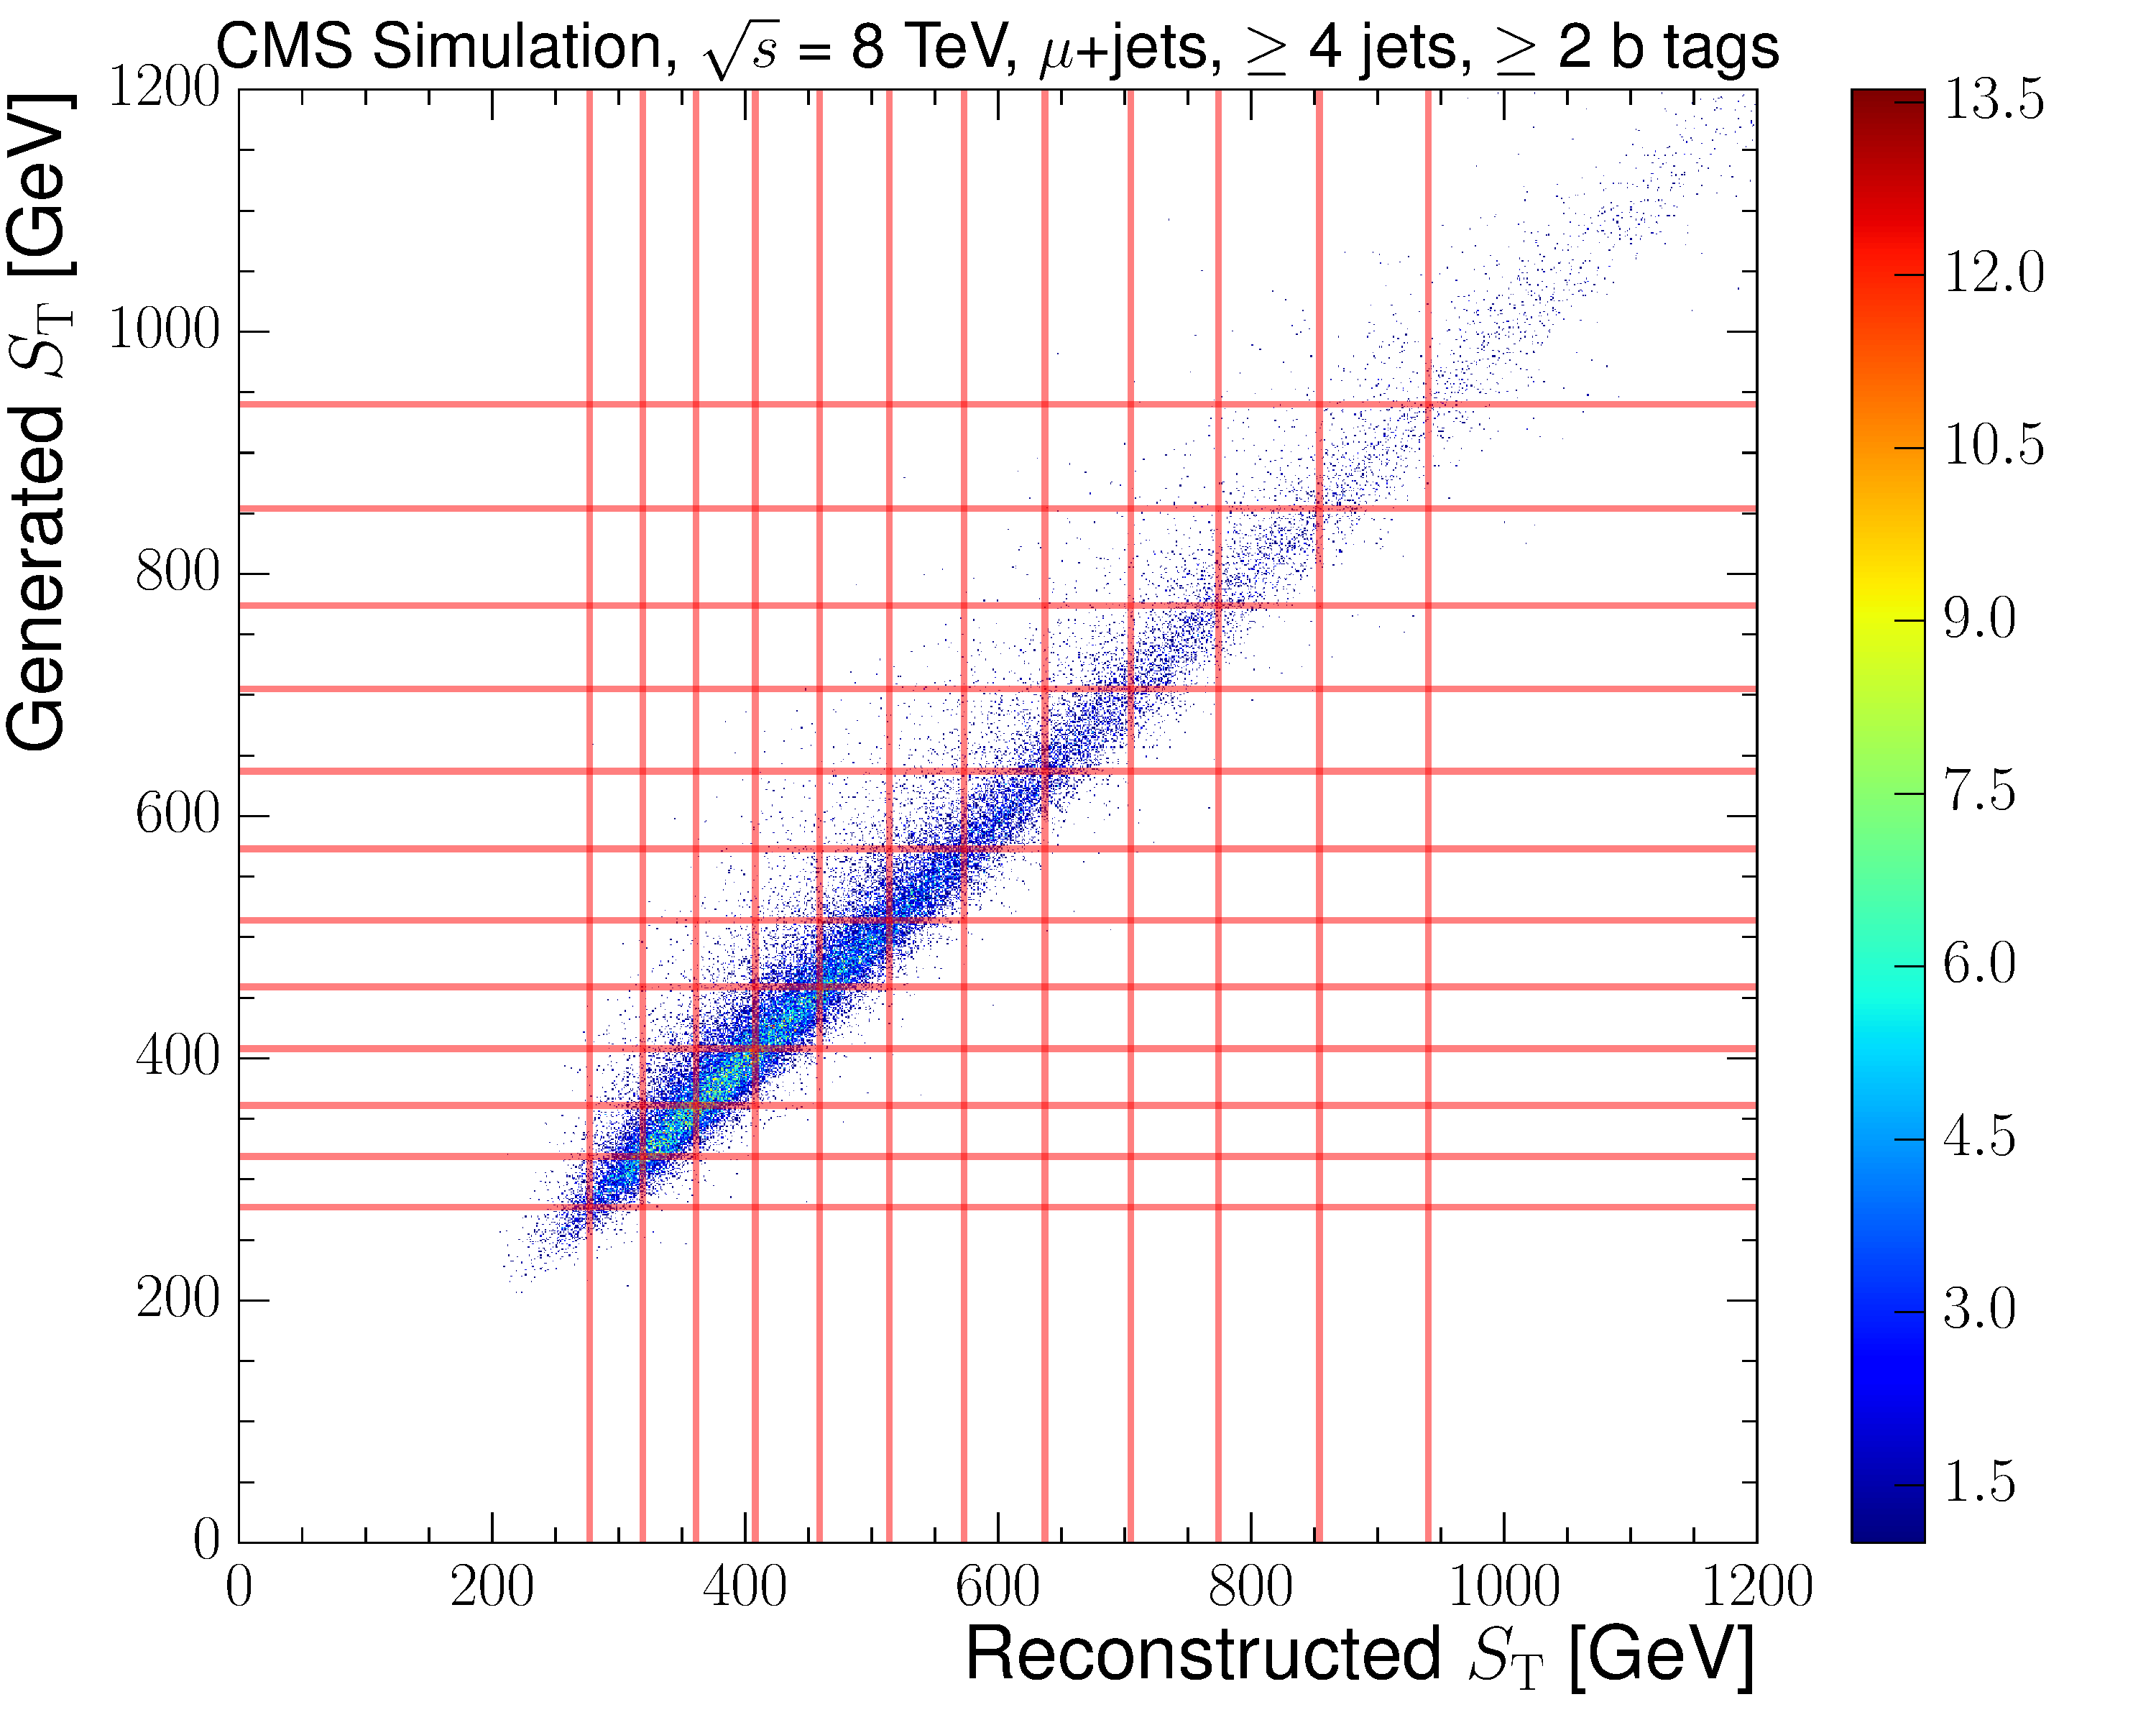
\includegraphics[width=0.48\textwidth]{Chapters/04_Analysis/04b_XSections/images/binning/muon_ST_8TeV.pdf}\hfill
     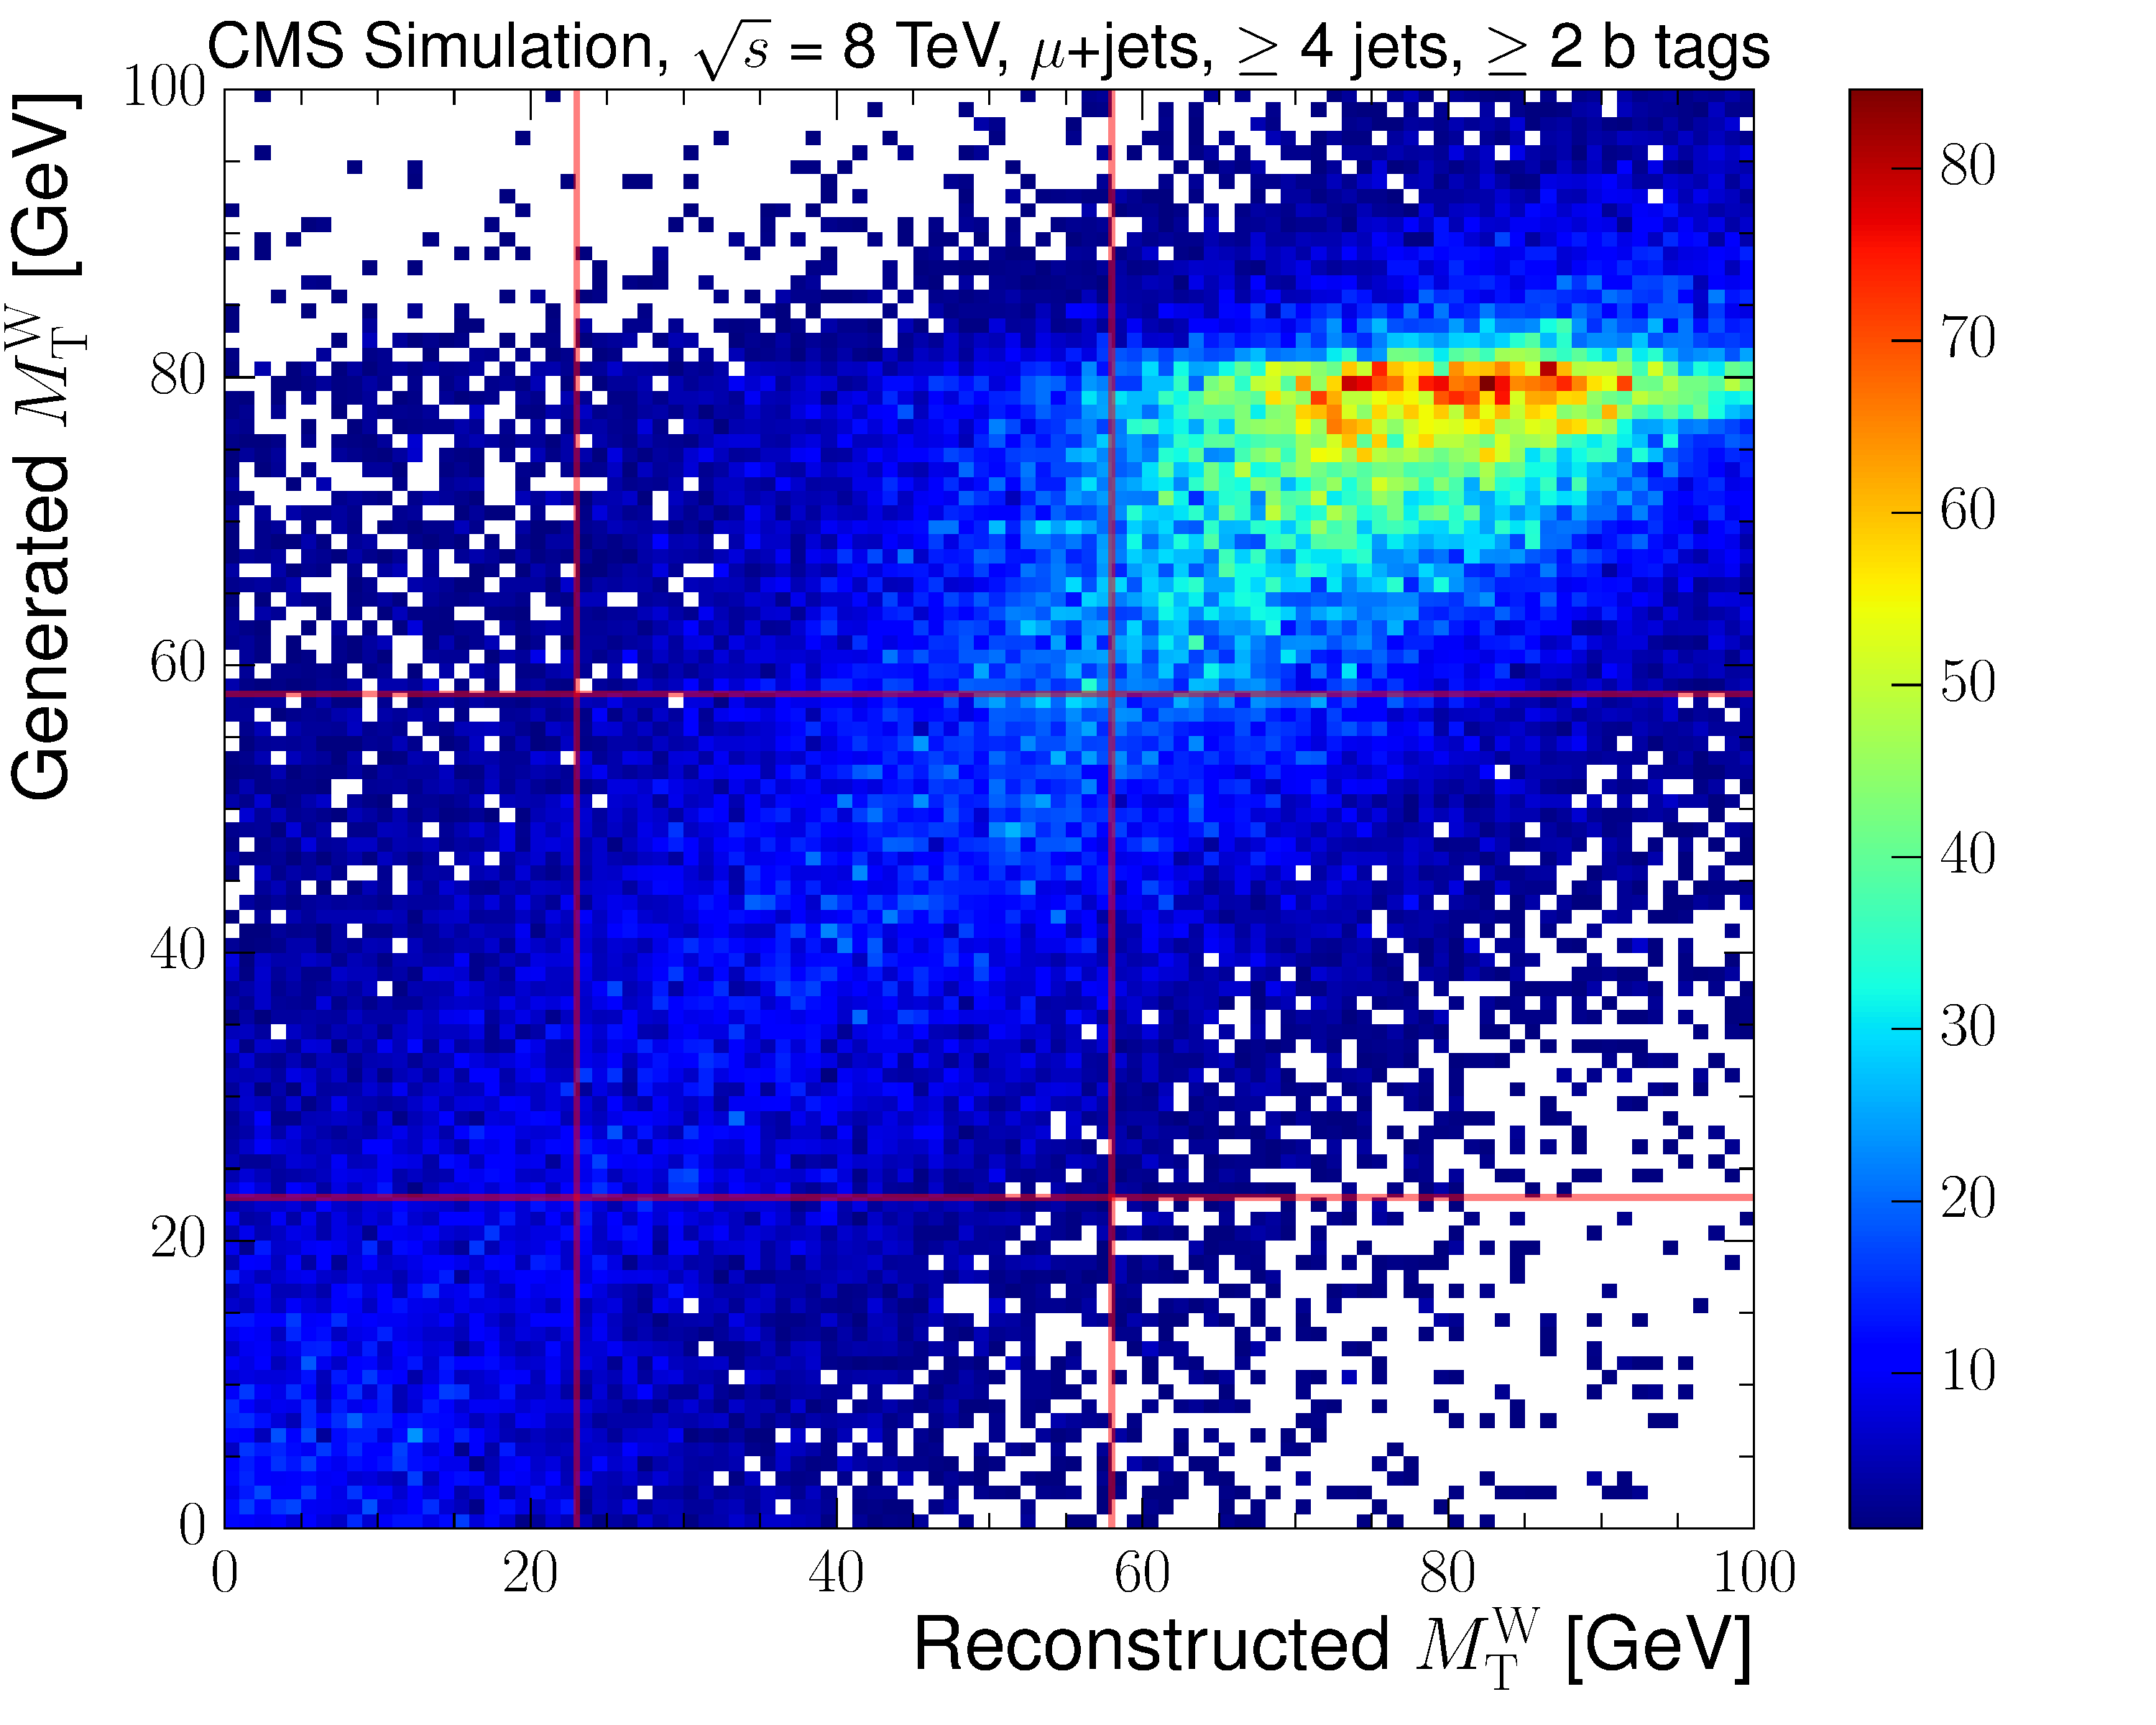
\includegraphics[width=0.48\textwidth]{Chapters/04_Analysis/04b_XSections/images/binning/muon_MT_8TeV.pdf}\\
	 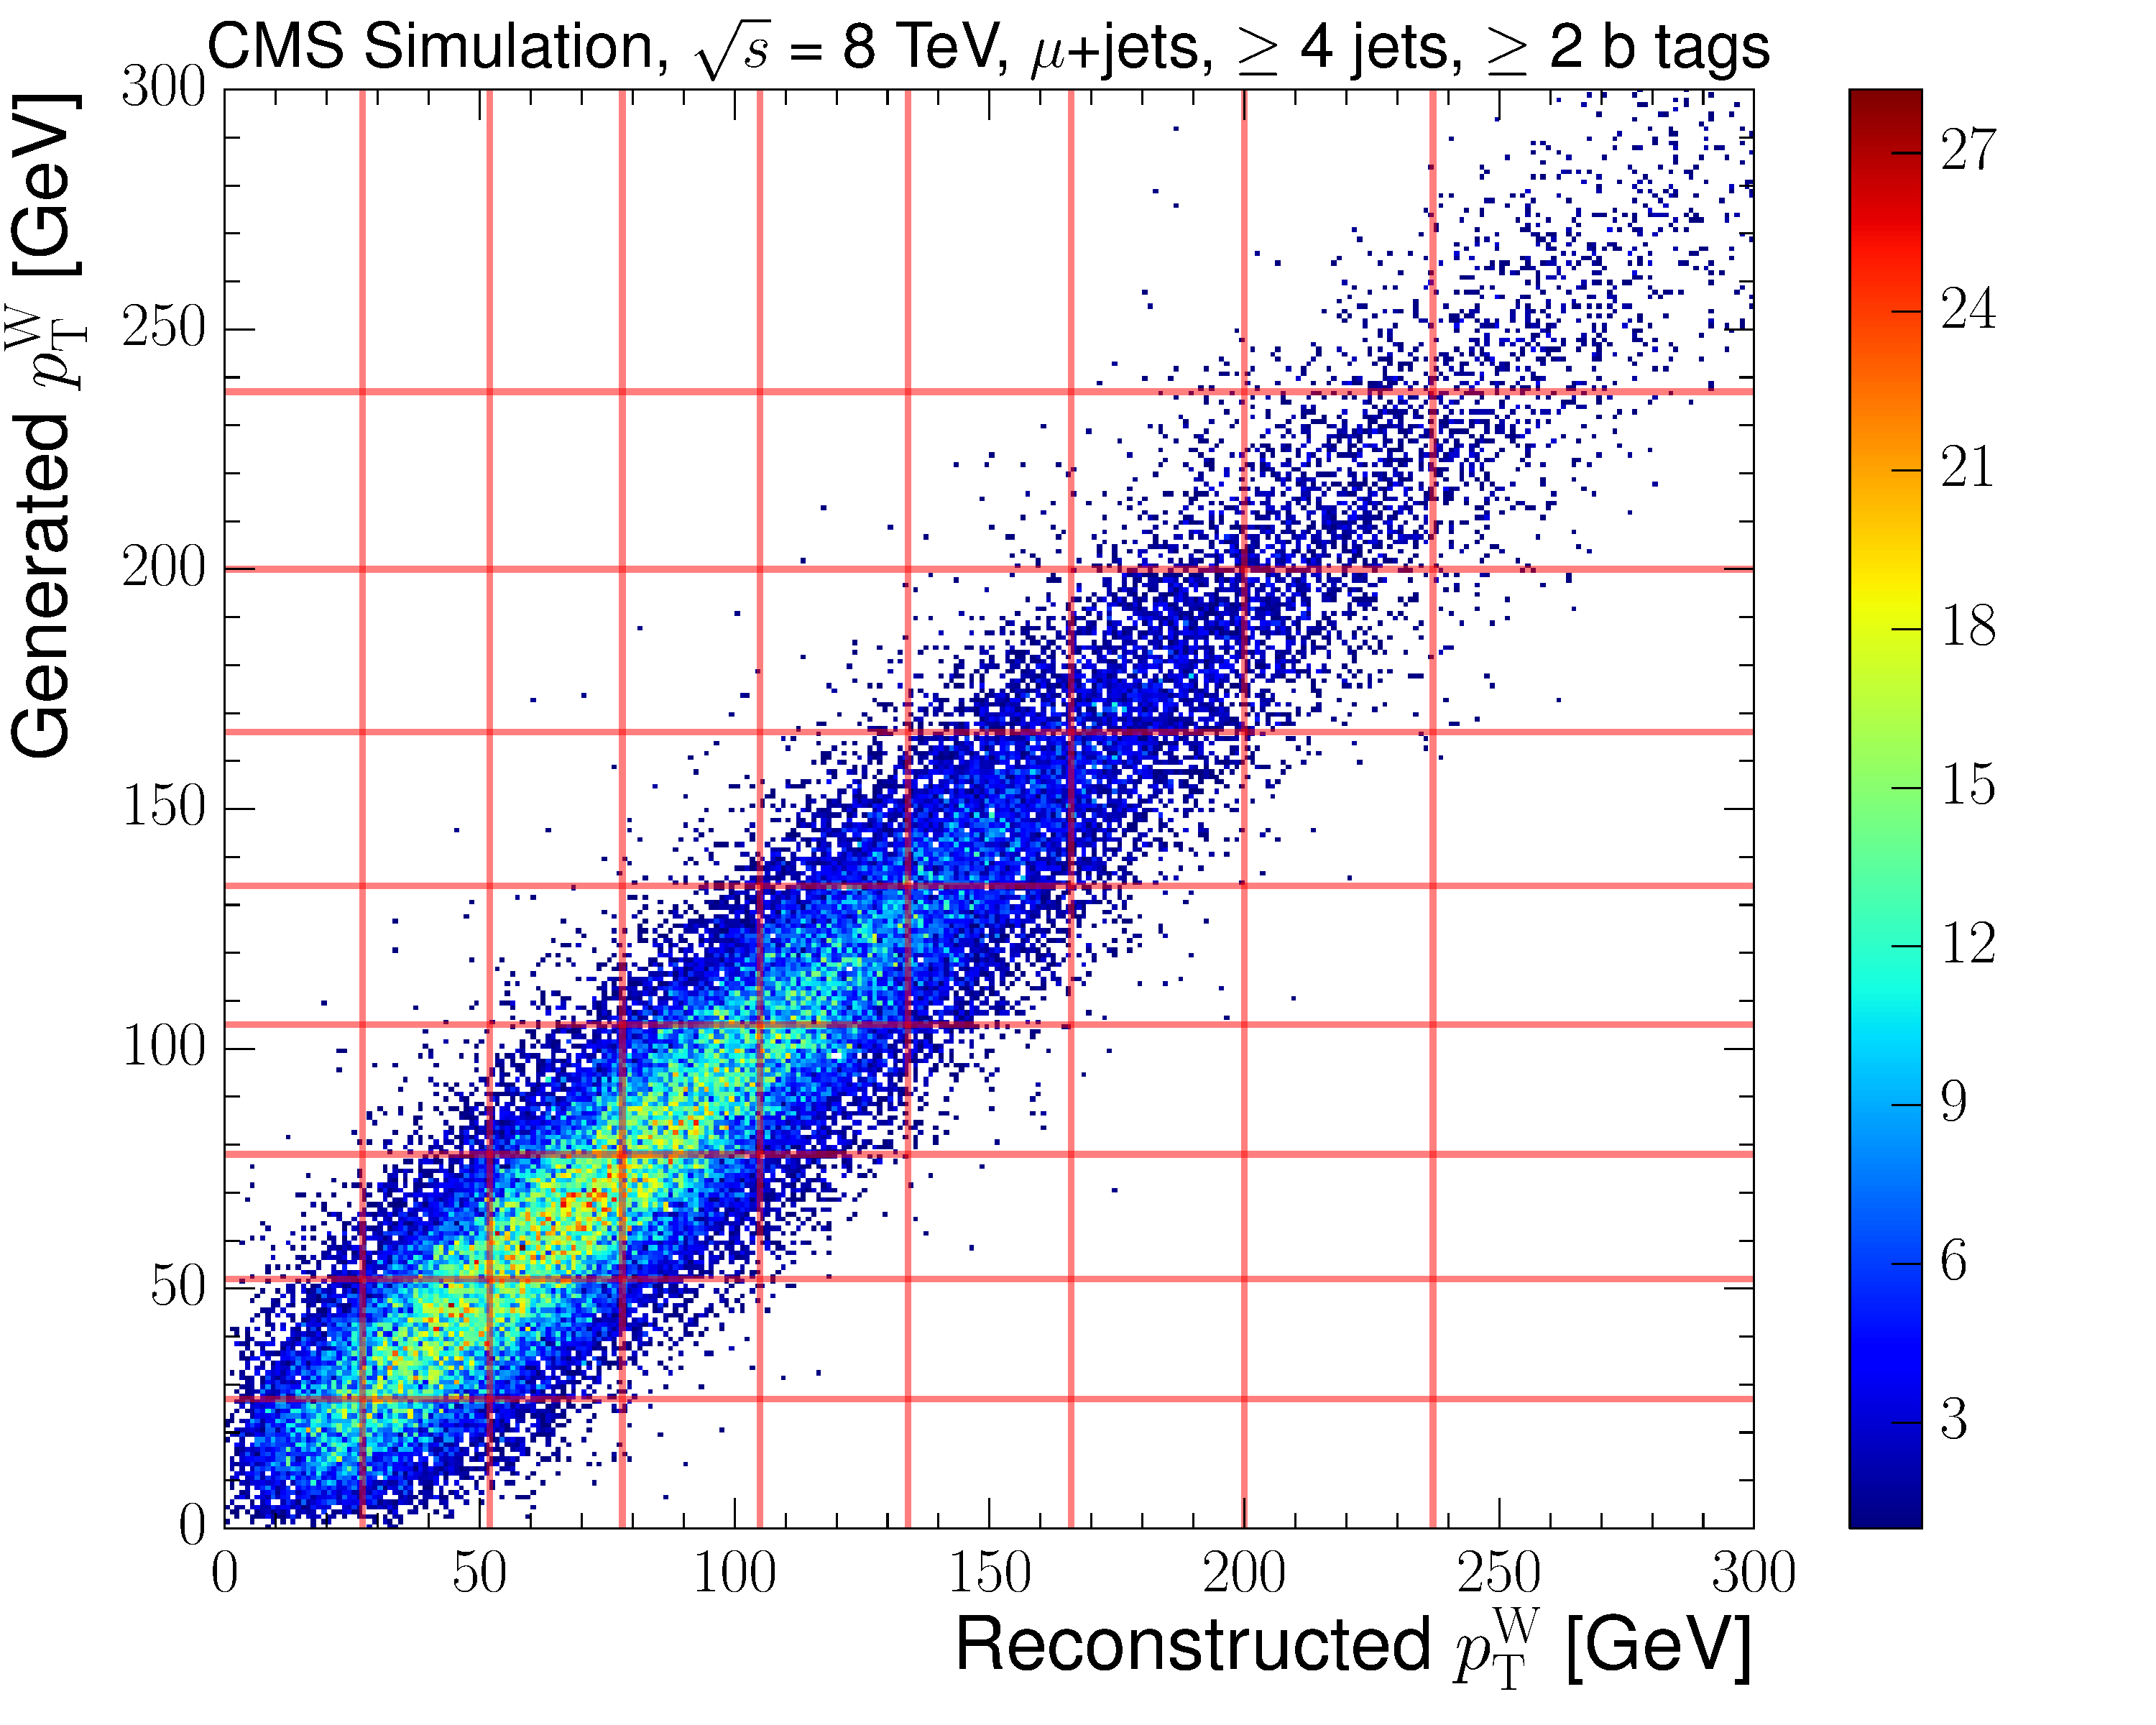
\includegraphics[width=0.48\textwidth]{Chapters/04_Analysis/04b_XSections/images/binning/muon_WPT_8TeV.pdf}\hfill
	 \caption{Generated versus reconstructed distributions of the primary variables \met (upper left), \HT (upper
	 right), \st (middle left), \mt (middle right) and \wpt (lower) with horizontal and vertical lines
	 representing the boundaries of the selected bins at $\sqrt{s}=8\TeV$ in the muon+jets channel. These
	 distributions are obtained using \ttbar Monte Carlo simulation.}
     \label{fig:binning_8TeV_muon}
 \end{figure}
 
\clearpage


\section{Binning choice tables}
\label{as:binning_tables_electron}

\begin{table}[ht]
\centering
\resizebox*{!}{\textheight} {
\begin{tabular}{lrrr}
\hline
\met bin (\GeV) &  purity & stability & number of events\\
\hline
0 - 27 & 0.649 & 0.533 & 1367\\
27 - 52 & 0.588 & 0.538 & 2187\\
52 - 87 & 0.537 & 0.636 & 1691\\
87 - 130 & 0.542 & 0.666 & 660\\
130 - 172 & 0.521 & 0.624 & 179\\
$\geq 172$ & 0.711 & 0.824 & 119\\
\hline
\HT bin (\GeV) &  purity & stability & number of events\\
\hline
0 - 186 & 0.589 & 0.567 & 102\\
186 - 216 & 0.546 & 0.565 & 344\\
216 - 249 & 0.542 & 0.585 & 676\\
249 - 286 & 0.541 & 0.575 & 884\\
286 - 326 & 0.543 & 0.556 & 896\\
326 - 368 & 0.536 & 0.538 & 765\\
368 - 412 & 0.537 & 0.517 & 598\\
412 - 462 & 0.566 & 0.538 & 518\\
462 - 516 & 0.573 & 0.531 & 375\\
516 - 574 & 0.580 & 0.537 & 264\\
574 - 634 & 0.590 & 0.529 & 172\\
634 - 696 & 0.581 & 0.539 & 113\\
696 - 781 & 0.660 & 0.624 & 100\\
$\geq 781$ & 0.886 & 0.814 & 117\\
\hline
\st bin (\GeV) &  purity & stability & number of events\\
\hline
0 - 277 & 0.565 & 0.550 & 108\\
277 - 319 & 0.564 & 0.549 & 422\\
319 - 361 & 0.538 & 0.543 & 743\\
361 - 408 & 0.530 & 0.547 & 939\\
408 - 459 & 0.527 & 0.539 & 897\\
459 - 514 & 0.534 & 0.536 & 764\\
514 - 573 & 0.539 & 0.530 & 601\\
573 - 637 & 0.548 & 0.532 & 449\\
637 - 705 & 0.548 & 0.534 & 305\\
705 - 774 & 0.540 & 0.523 & 194\\
774 - 854 & 0.576 & 0.566 & 151\\
854 - 946 & 0.613 & 0.580 & 102\\
$\geq 946$ & 0.838 & 0.837 & 133\\
\hline
\mt bin (\GeV) &  purity & stability & number of events\\
\hline
0 - 23 & 0.528 & 0.598 & 659\\
23 - 58 & 0.515 & 0.562 & 1557\\
$\geq 58$ & 0.845 & 0.786 & 4518\\
\hline
\wpt bin (\GeV) &  purity & stability & number of events\\
\hline
0 - 27 & 0.597 & 0.549 & 467\\
27 - 52 & 0.551 & 0.526 & 960\\
52 - 78 & 0.550 & 0.540 & 1228\\
78 - 105 & 0.539 & 0.538 & 1107\\
105 - 134 & 0.537 & 0.554 & 857\\
134 - 166 & 0.537 & 0.568 & 570\\
166 - 200 & 0.524 & 0.564 & 314\\
200 - 237 & 0.536 & 0.573 & 177\\
$\geq 237$ & 0.707 & 0.789 & 145\\
\hline
\end{tabular}
}
\caption{The selected bins for the measurement in the electron channel at a centre-of-mass energy of 7\TeV. In addition
to the bin ranges the purity, stability and number of expected \ttbar events are shown.}
\label{tab:binning_electron_7TeV}
\end{table}

\begin{table}[ht]
\centering
\begin{tabular}{lrrr}
\hline

\met bin (\GeV) &  purity & stability & number of events\\
\hline
0 - 27 & 0.641 & 0.533 & 1445\\
27 - 52 & 0.587 & 0.536 & 2374\\
52 - 87 & 0.552 & 0.638 & 1982\\
87 - 130 & 0.550 & 0.673 & 770\\
130 - 172 & 0.533 & 0.634 & 207\\
$\geq 172$ & 0.706 & 0.844 & 133\\
\hline
\HT bin (\GeV) &  purity & stability & number of events\\
\hline
0 - 186 & 0.595 & 0.568 & 121\\
186 - 216 & 0.543 & 0.563 & 397\\
216 - 249 & 0.545 & 0.583 & 787\\
249 - 286 & 0.541 & 0.576 & 1008\\
286 - 326 & 0.546 & 0.559 & 1010\\
326 - 368 & 0.540 & 0.538 & 841\\
368 - 412 & 0.547 & 0.529 & 675\\
412 - 462 & 0.569 & 0.542 & 558\\
462 - 516 & 0.584 & 0.537 & 406\\
516 - 574 & 0.585 & 0.547 & 281\\
574 - 634 & 0.590 & 0.542 & 181\\
634 - 696 & 0.597 & 0.546 & 119\\
696 - 781 & 0.682 & 0.623 & 105\\
$\geq 781$ & 0.885 & 0.818 & 117\\
\hline
\st bin (\GeV) &  purity & stability & number of events\\
\hline
0 - 277 & 0.562 & 0.552 & 135\\
277 - 319 & 0.560 & 0.542 & 503\\
319 - 361 & 0.536 & 0.546 & 866\\
361 - 408 & 0.532 & 0.546 & 1056\\
408 - 459 & 0.530 & 0.543 & 1003\\
459 - 514 & 0.538 & 0.540 & 853\\
514 - 573 & 0.543 & 0.531 & 645\\
573 - 637 & 0.553 & 0.534 & 477\\
637 - 705 & 0.548 & 0.539 & 326\\
705 - 774 & 0.542 & 0.523 & 200\\
774 - 854 & 0.571 & 0.557 & 152\\
854 - 946 & 0.598 & 0.585 & 101\\
$\geq 946$ & 0.847 & 0.832 & 138\\
\hline
\mt bin (\GeV) &  purity & stability & number of events\\
\hline
0 - 23 & 0.535 & 0.608 & 742\\
23 - 58 & 0.523 & 0.574 & 1777\\
$\geq 58$ & 0.851 & 0.789 & 5093\\
\hline
\wpt bin (\GeV) &  purity & stability & number of events\\
\hline
0 - 27 & 0.599 & 0.544 & 558\\
27 - 52 & 0.559 & 0.529 & 1141\\
52 - 78 & 0.549 & 0.539 & 1369\\
78 - 105 & 0.531 & 0.538 & 1190\\
105 - 134 & 0.537 & 0.557 & 928\\
134 - 166 & 0.537 & 0.569 & 610\\
166 - 200 & 0.526 & 0.568 & 336\\
200 - 237 & 0.532 & 0.575 & 183\\
$\geq 237$ & 0.689 & 0.794 & 150\\
\hline
\end{tabular}
\caption{The selected bins for the measurement in the muon channel at a centre-of-mass energy of 7\TeV. In addition
to the bin ranges the purity, stability and number of expected \ttbar events are shown.}
\label{tab:binning_muon_7TeV}
\end{table}

\begin{table}[ht]
\centering
\resizebox*{!}{\textheight} {
\begin{tabular}{lrrr}
\hline
\met bin (\GeV) &  purity & stability & number of events\\
\hline
0 - 27 & 0.634 & 0.505 & 6400\\
27 - 52 & 0.557 & 0.507 & 9823\\
52 - 87 & 0.503 & 0.606 & 7792\\
87 - 130 & 0.517 & 0.643 & 3239\\
130 - 172 & 0.500 & 0.598 & 904\\
$\geq 172$ & 0.700 & 0.840 & 670\\
\hline
\HT bin (\GeV) &  purity & stability & number of events\\
\hline
0 - 186 & 0.556 & 0.514 & 430\\
186 - 216 & 0.511 & 0.508 & 1408\\
216 - 249 & 0.508 & 0.540 & 2878\\
249 - 286 & 0.511 & 0.540 & 3869\\
286 - 326 & 0.502 & 0.524 & 3892\\
326 - 368 & 0.508 & 0.511 & 3463\\
368 - 412 & 0.506 & 0.500 & 2828\\
412 - 462 & 0.532 & 0.510 & 2457\\
462 - 516 & 0.534 & 0.509 & 1857\\
516 - 574 & 0.547 & 0.500 & 1256\\
574 - 634 & 0.557 & 0.512 & 902\\
634 - 696 & 0.518 & 0.505 & 584\\
696 - 781 & 0.627 & 0.551 & 572\\
$\geq 781$ & 0.872 & 0.815 & 801\\
\hline
\st bin (\GeV) &  purity & stability & number of events\\
\hline
0 - 277 & 0.580 & 0.500 & 463\\
277 - 319 & 0.539 & 0.500 & 1769\\
319 - 361 & 0.509 & 0.515 & 3204\\
361 - 408 & 0.505 & 0.522 & 4126\\
408 - 459 & 0.501 & 0.514 & 4035\\
459 - 514 & 0.504 & 0.510 & 3532\\
514 - 573 & 0.503 & 0.502 & 2780\\
573 - 637 & 0.517 & 0.510 & 2179\\
637 - 705 & 0.517 & 0.504 & 1507\\
705 - 774 & 0.506 & 0.508 & 1039\\
774 - 854 & 0.540 & 0.504 & 769\\
854 - 946 & 0.552 & 0.550 & 551\\
$\geq 946$ & 0.842 & 0.831 & 909\\
\hline
\mt bin (\GeV) &  purity & stability & number of events\\
\hline
0 - 23 & 0.515 & 0.577 & 3245\\
23 - 58 & 0.507 & 0.541 & 7446\\
$\geq 58$ & 0.823 & 0.774 & 20751\\
\hline
\wpt bin (\GeV) &  purity & stability & number of events\\
\hline
0 - 27 & 0.556 & 0.505 & 1962\\
27 - 52 & 0.531 & 0.507 & 4354\\
52 - 78 & 0.527 & 0.513 & 5536\\
78 - 105 & 0.515 & 0.510 & 5131\\
105 - 134 & 0.510 & 0.533 & 4051\\
134 - 166 & 0.518 & 0.546 & 2775\\
166 - 200 & 0.502 & 0.544 & 1590\\
200 - 237 & 0.511 & 0.545 & 903\\
$\geq 237$ & 0.683 & 0.790 & 792\\
\hline
\end{tabular}
}
\caption{The selected bins for the measurement in the electron channel at a centre-of-mass energy of 8\TeV. In addition
to the bin ranges the purity, stability and number of expected \ttbar events are shown.}
\label{tab:binning_electron_8TeV}
\end{table}

\begin{table}[ht]
\centering
\begin{tabular}{lrrr}
\hline

\met bin (\GeV) &  purity & stability & number of events\\
\hline
0 - 27 & 0.638 & 0.511 & 7341\\
27 - 52 & 0.563 & 0.515 & 11569\\
52 - 87 & 0.526 & 0.610 & 9865\\
87 - 130 & 0.506 & 0.651 & 3814\\
130 - 172 & 0.504 & 0.592 & 1050\\
$\geq 172$ & 0.695 & 0.845 & 802\\
\hline
\HT bin (\GeV) &  purity & stability & number of events\\
\hline
0 - 186 & 0.559 & 0.514 & 527\\
186 - 216 & 0.518 & 0.515 & 1698\\
216 - 249 & 0.518 & 0.537 & 3521\\
249 - 286 & 0.507 & 0.548 & 4735\\
286 - 326 & 0.507 & 0.523 & 4725\\
326 - 368 & 0.500 & 0.504 & 4032\\
368 - 412 & 0.503 & 0.501 & 3297\\
412 - 462 & 0.536 & 0.503 & 2815\\
462 - 516 & 0.529 & 0.503 & 2087\\
516 - 574 & 0.549 & 0.520 & 1551\\
574 - 634 & 0.542 & 0.502 & 987\\
634 - 696 & 0.560 & 0.504 & 656\\
696 - 781 & 0.644 & 0.607 & 641\\
$\geq 781$ & 0.886 & 0.796 & 842\\
\hline
\st bin (\GeV) &  purity & stability & number of events\\
\hline
0 - 277 & 0.583 & 0.523 & 629\\
277 - 319 & 0.548 & 0.519 & 2276\\
319 - 361 & 0.511 & 0.508 & 3895\\
361 - 408 & 0.504 & 0.522 & 5021\\
408 - 459 & 0.502 & 0.519 & 4855\\
459 - 514 & 0.508 & 0.512 & 4170\\
514 - 573 & 0.511 & 0.500 & 3248\\
573 - 637 & 0.502 & 0.504 & 2393\\
637 - 705 & 0.522 & 0.517 & 1766\\
705 - 774 & 0.519 & 0.500 & 1135\\
774 - 854 & 0.546 & 0.529 & 884\\
854 - 946 & 0.571 & 0.558 & 621\\
$\geq 946$ & 0.836 & 0.837 & 961\\
\hline
\mt bin (\GeV) &  purity & stability & number of events\\
\hline
0 - 23 & 0.506 & 0.589 & 3712\\
23 - 58 & 0.511 & 0.554 & 9078\\
$\geq 58$ & 0.836 & 0.774 & 25227\\
\hline
\wpt bin (\GeV) &  purity & stability & number of events\\
\hline
0 - 27 & 0.589 & 0.520 & 2700\\
27 - 52 & 0.535 & 0.509 & 5484\\
52 - 78 & 0.524 & 0.509 & 6644\\
78 - 105 & 0.507 & 0.515 & 5918\\
105 - 134 & 0.509 & 0.526 & 4588\\
134 - 166 & 0.504 & 0.544 & 3012\\
166 - 200 & 0.513 & 0.546 & 1767\\
200 - 237 & 0.506 & 0.558 & 994\\
$\geq 237$ & 0.676 & 0.801 & 894\\
\hline
\end{tabular}
\caption{The selected bins for the measurement in the muon channel at a centre-of-mass energy of 8\TeV. In addition
to the bin ranges the purity, stability and number of expected \ttbar events are shown.}
\label{tab:binning_muon_8TeV}
\end{table}


\clearpage


\section{Fitting Variable Distributions}
\label{as:fitting_variables_distributions}
\begin{figure}[hbtp]
    \centering
     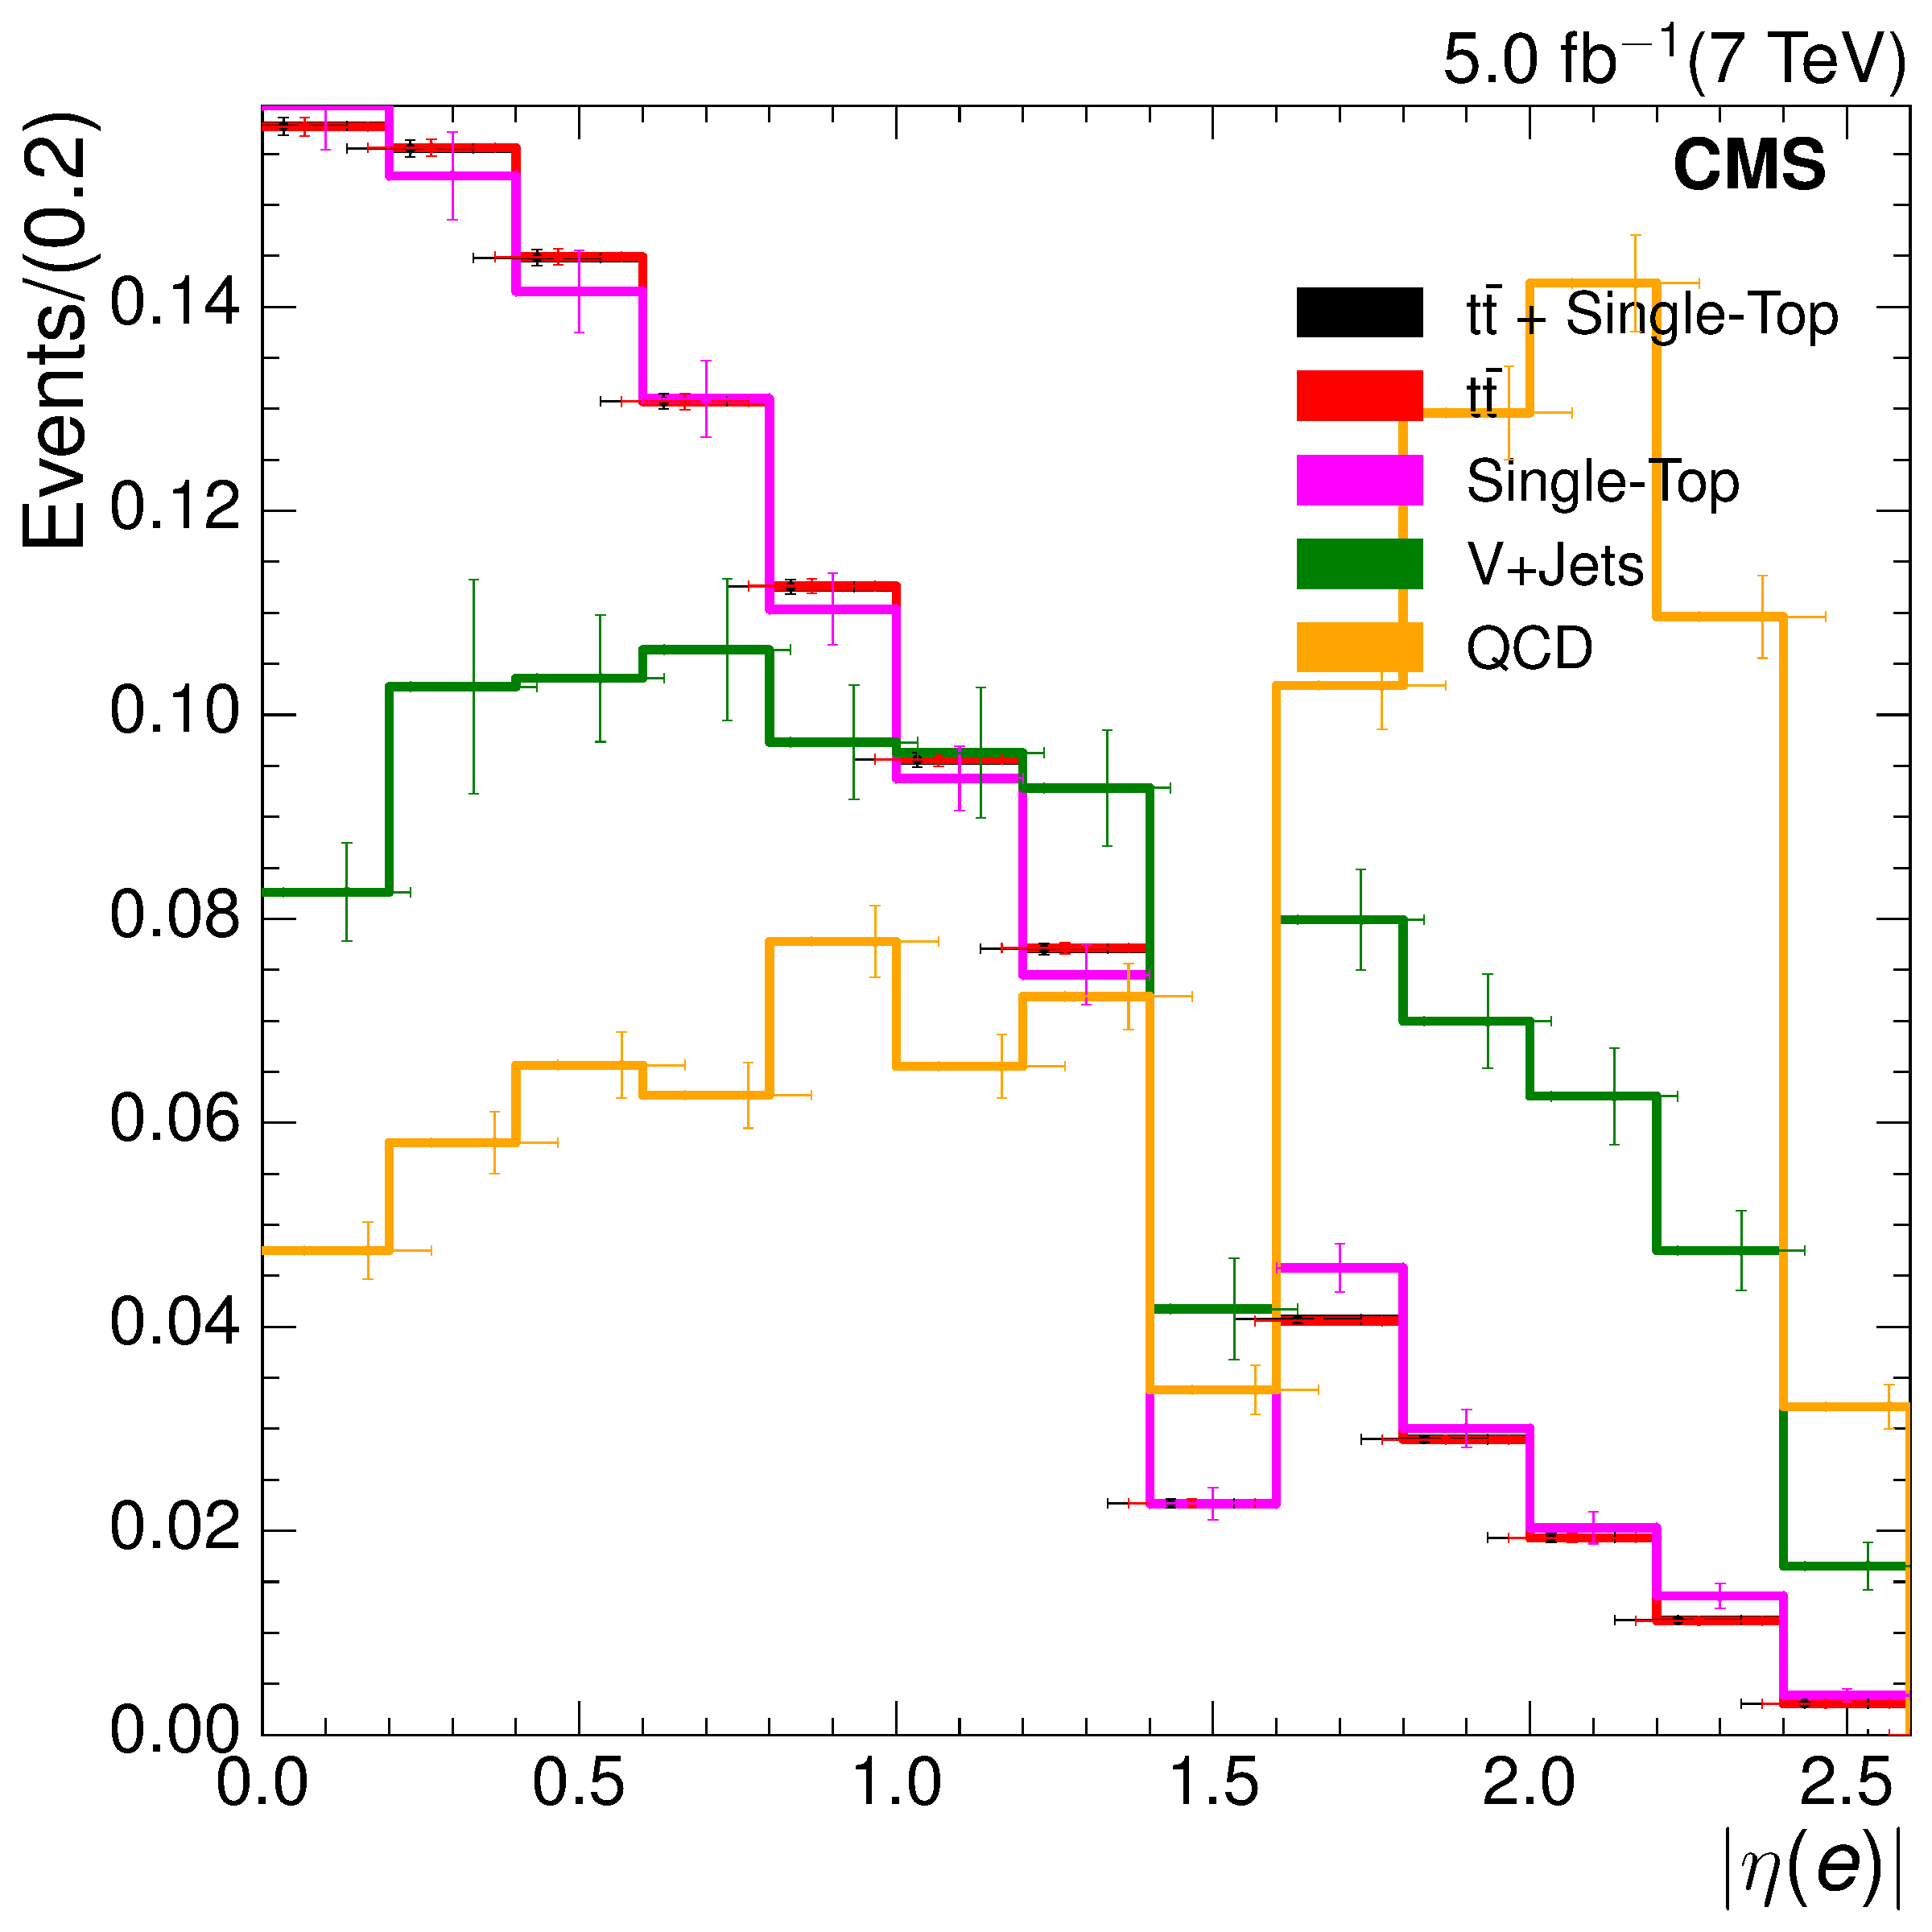
\includegraphics[width=0.48\textwidth]{Chapters/04_Analysis/04b_XSections/images/8TeV/fit_variables/electron/MET/electron_absolute_eta/MET_inclusive_electron_absolute_eta_2orMoreBtags_templates.pdf}\hfill
     \includegraphics[width=0.48\textwidth]{Chapters/04_Analysis/04b_XSections/images/8TeV/fit_variables/electron/MET/angle_bl/MET_inclusive_angle_bl_2orMoreBtags_templates.pdf}
     \includegraphics[width=0.48\textwidth]{Chapters/04_Analysis/04b_XSections/images/8TeV/fit_variables/electron/MET/M3/MET_inclusive_M3_2orMoreBtags_templates.pdf}\\
	 \caption{Normalised distributions of the templates for the three fit variables at $\sqrt{s}=8\TeV$,
	 inclusive across all primary variable bins in the electron+jets channel: electron \abseta (upper left),
	 $\alpha$ (upper right) and M3 (lower).}
     \label{fig:fit_variable_distributions_electron_8TeV}
\end{figure}

\begin{figure}[hbtp]
    \centering
     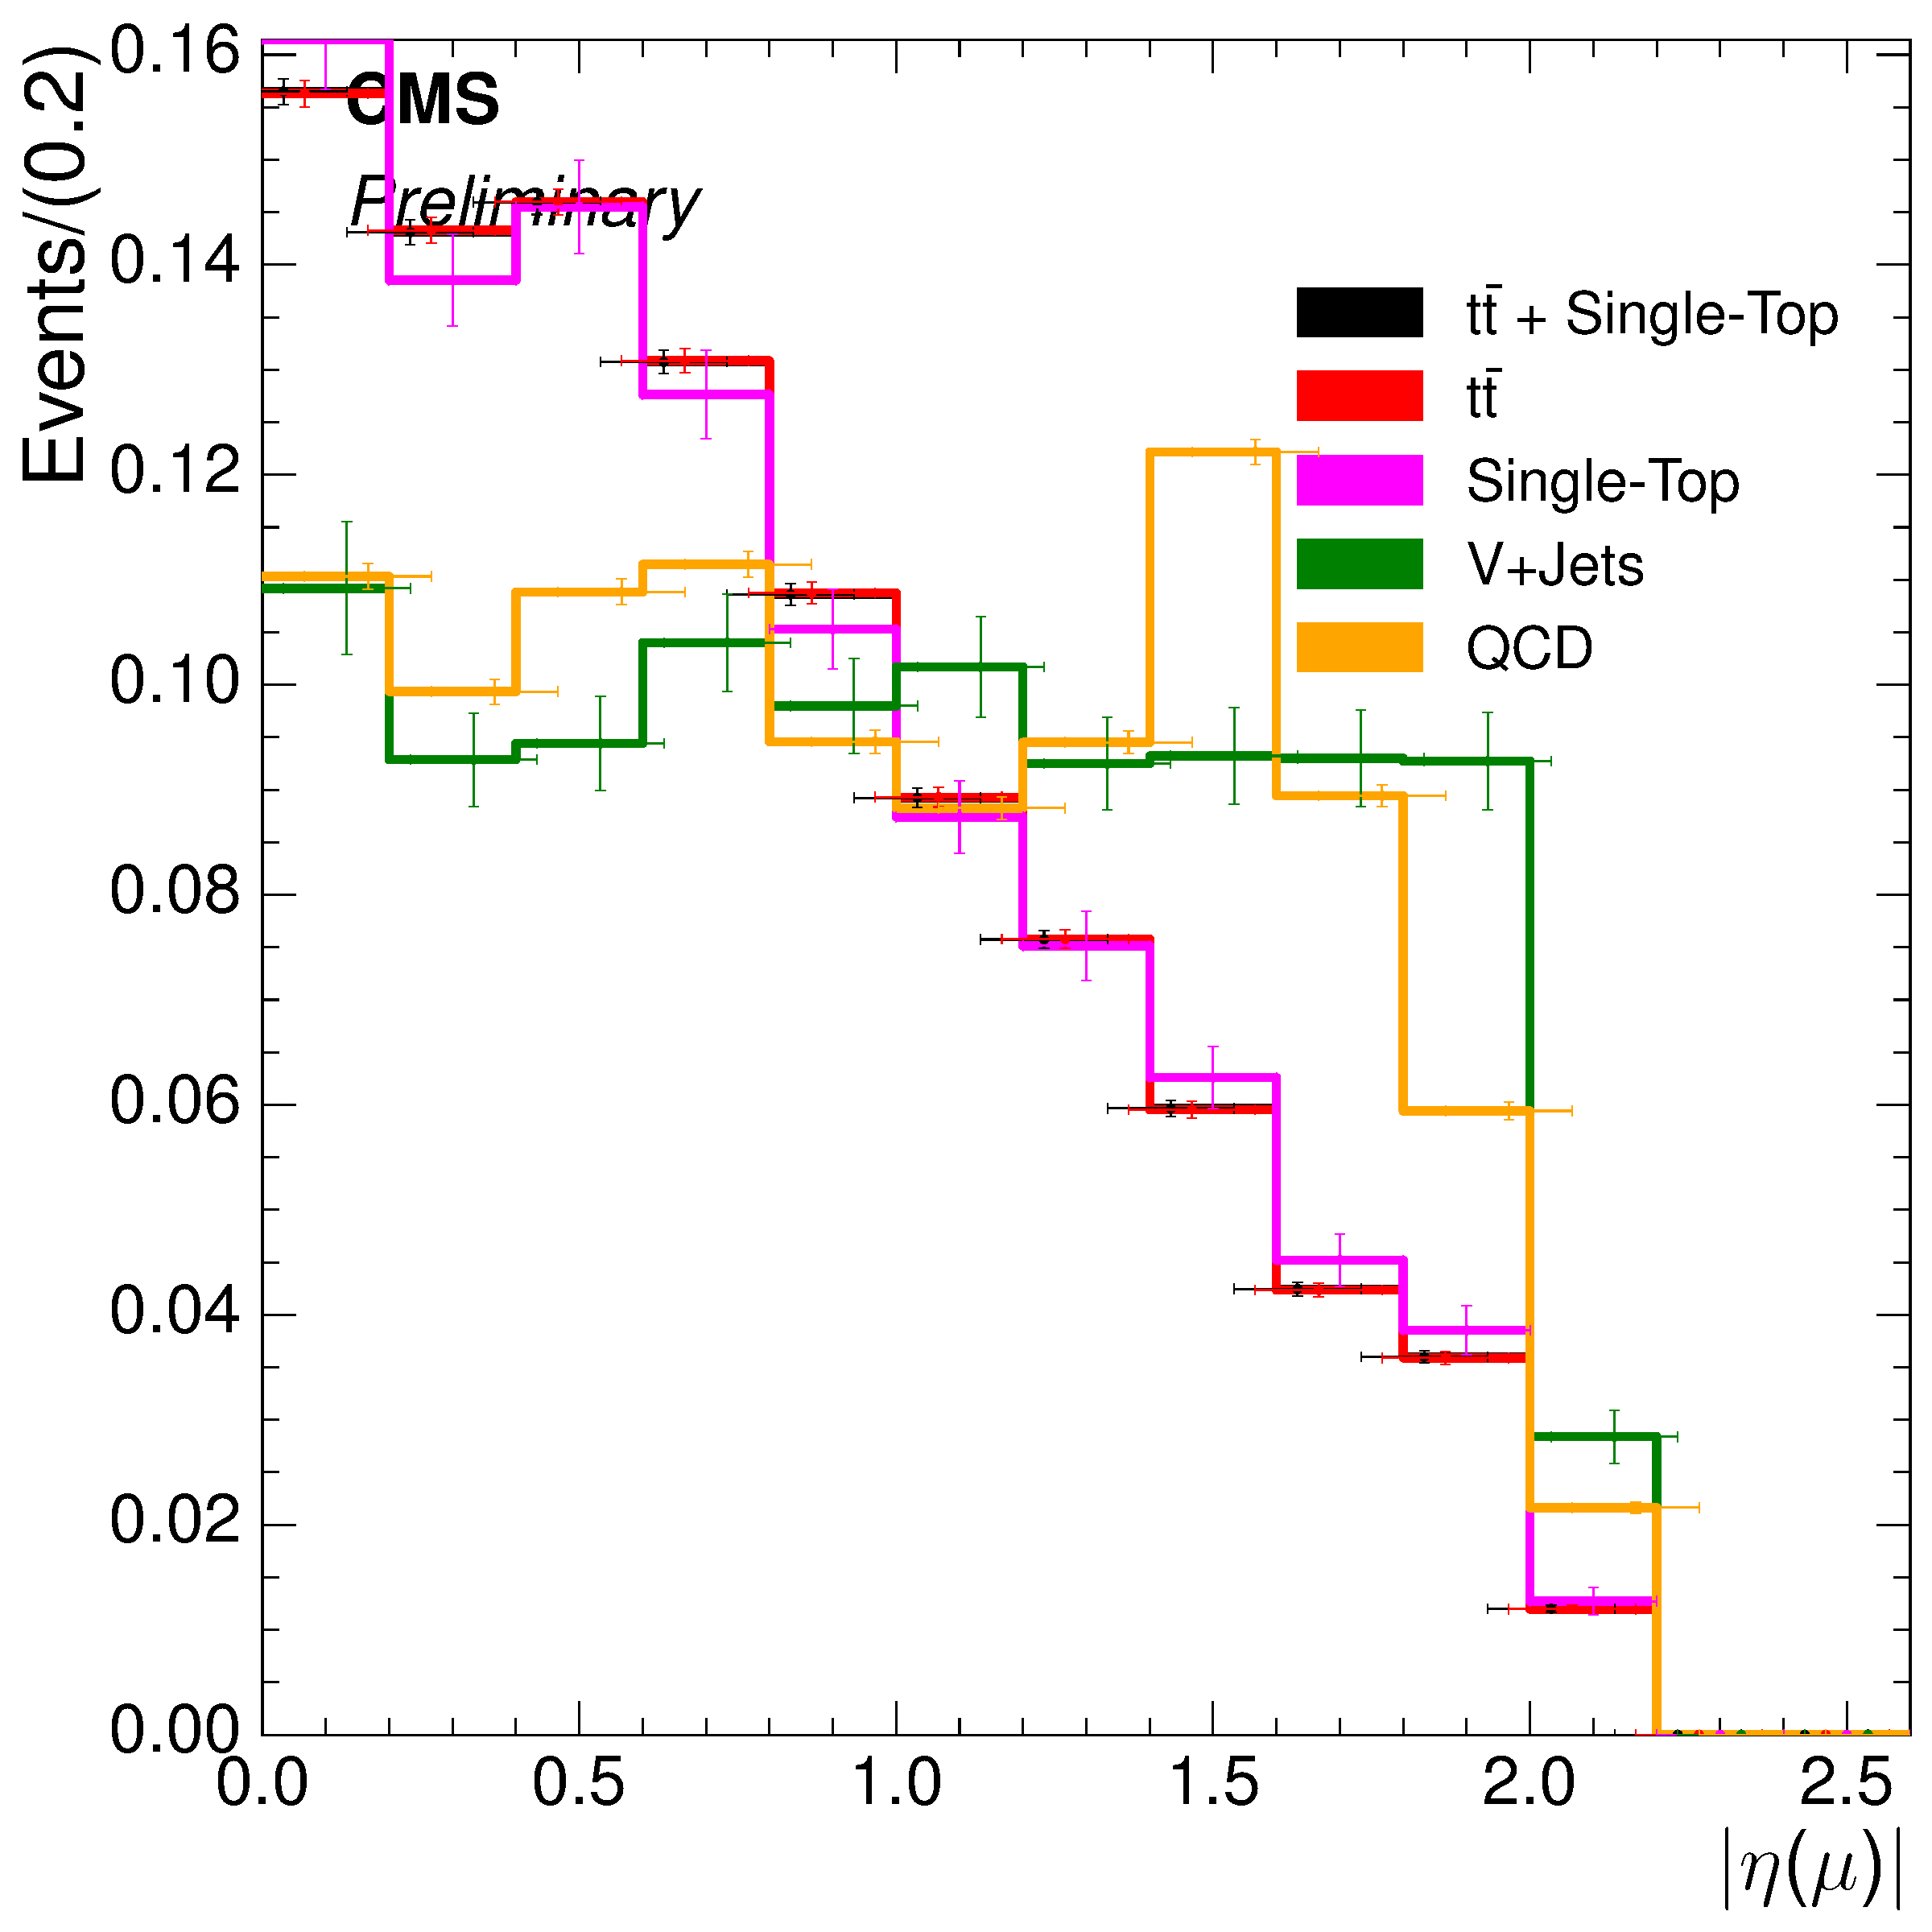
\includegraphics[width=0.48\textwidth]{Chapters/04_Analysis/04b_XSections/images/8TeV/fit_variables/muon/MET/muon_absolute_eta/MET_inclusive_muon_absolute_eta_2orMoreBtags_templates.pdf}\hfill
     \includegraphics[width=0.48\textwidth]{Chapters/04_Analysis/04b_XSections/images/8TeV/fit_variables/muon/MET/angle_bl/MET_inclusive_angle_bl_2orMoreBtags_templates.pdf}
     \includegraphics[width=0.48\textwidth]{Chapters/04_Analysis/04b_XSections/images/8TeV/fit_variables/muon/MET/M3/MET_inclusive_M3_2orMoreBtags_templates.pdf}\\
	 \caption{Normalised distributions of the templates for the three fit variables at $\sqrt{s}=8\TeV$,
	 inclusive across all primary variable bins in the muon+jets channel: muon \abseta (upper left),
	 $\alpha$ (upper right) and M3 (lower).}
     \label{fig:fit_variable_distributions_muon_8TeV}
\end{figure}

\clearpage


\section{Fitting variable QCD background template comparisons}
\label{as:fitting_variable_QCD_template_comparisons}

\begin{figure}[hbtp]
    \centering
     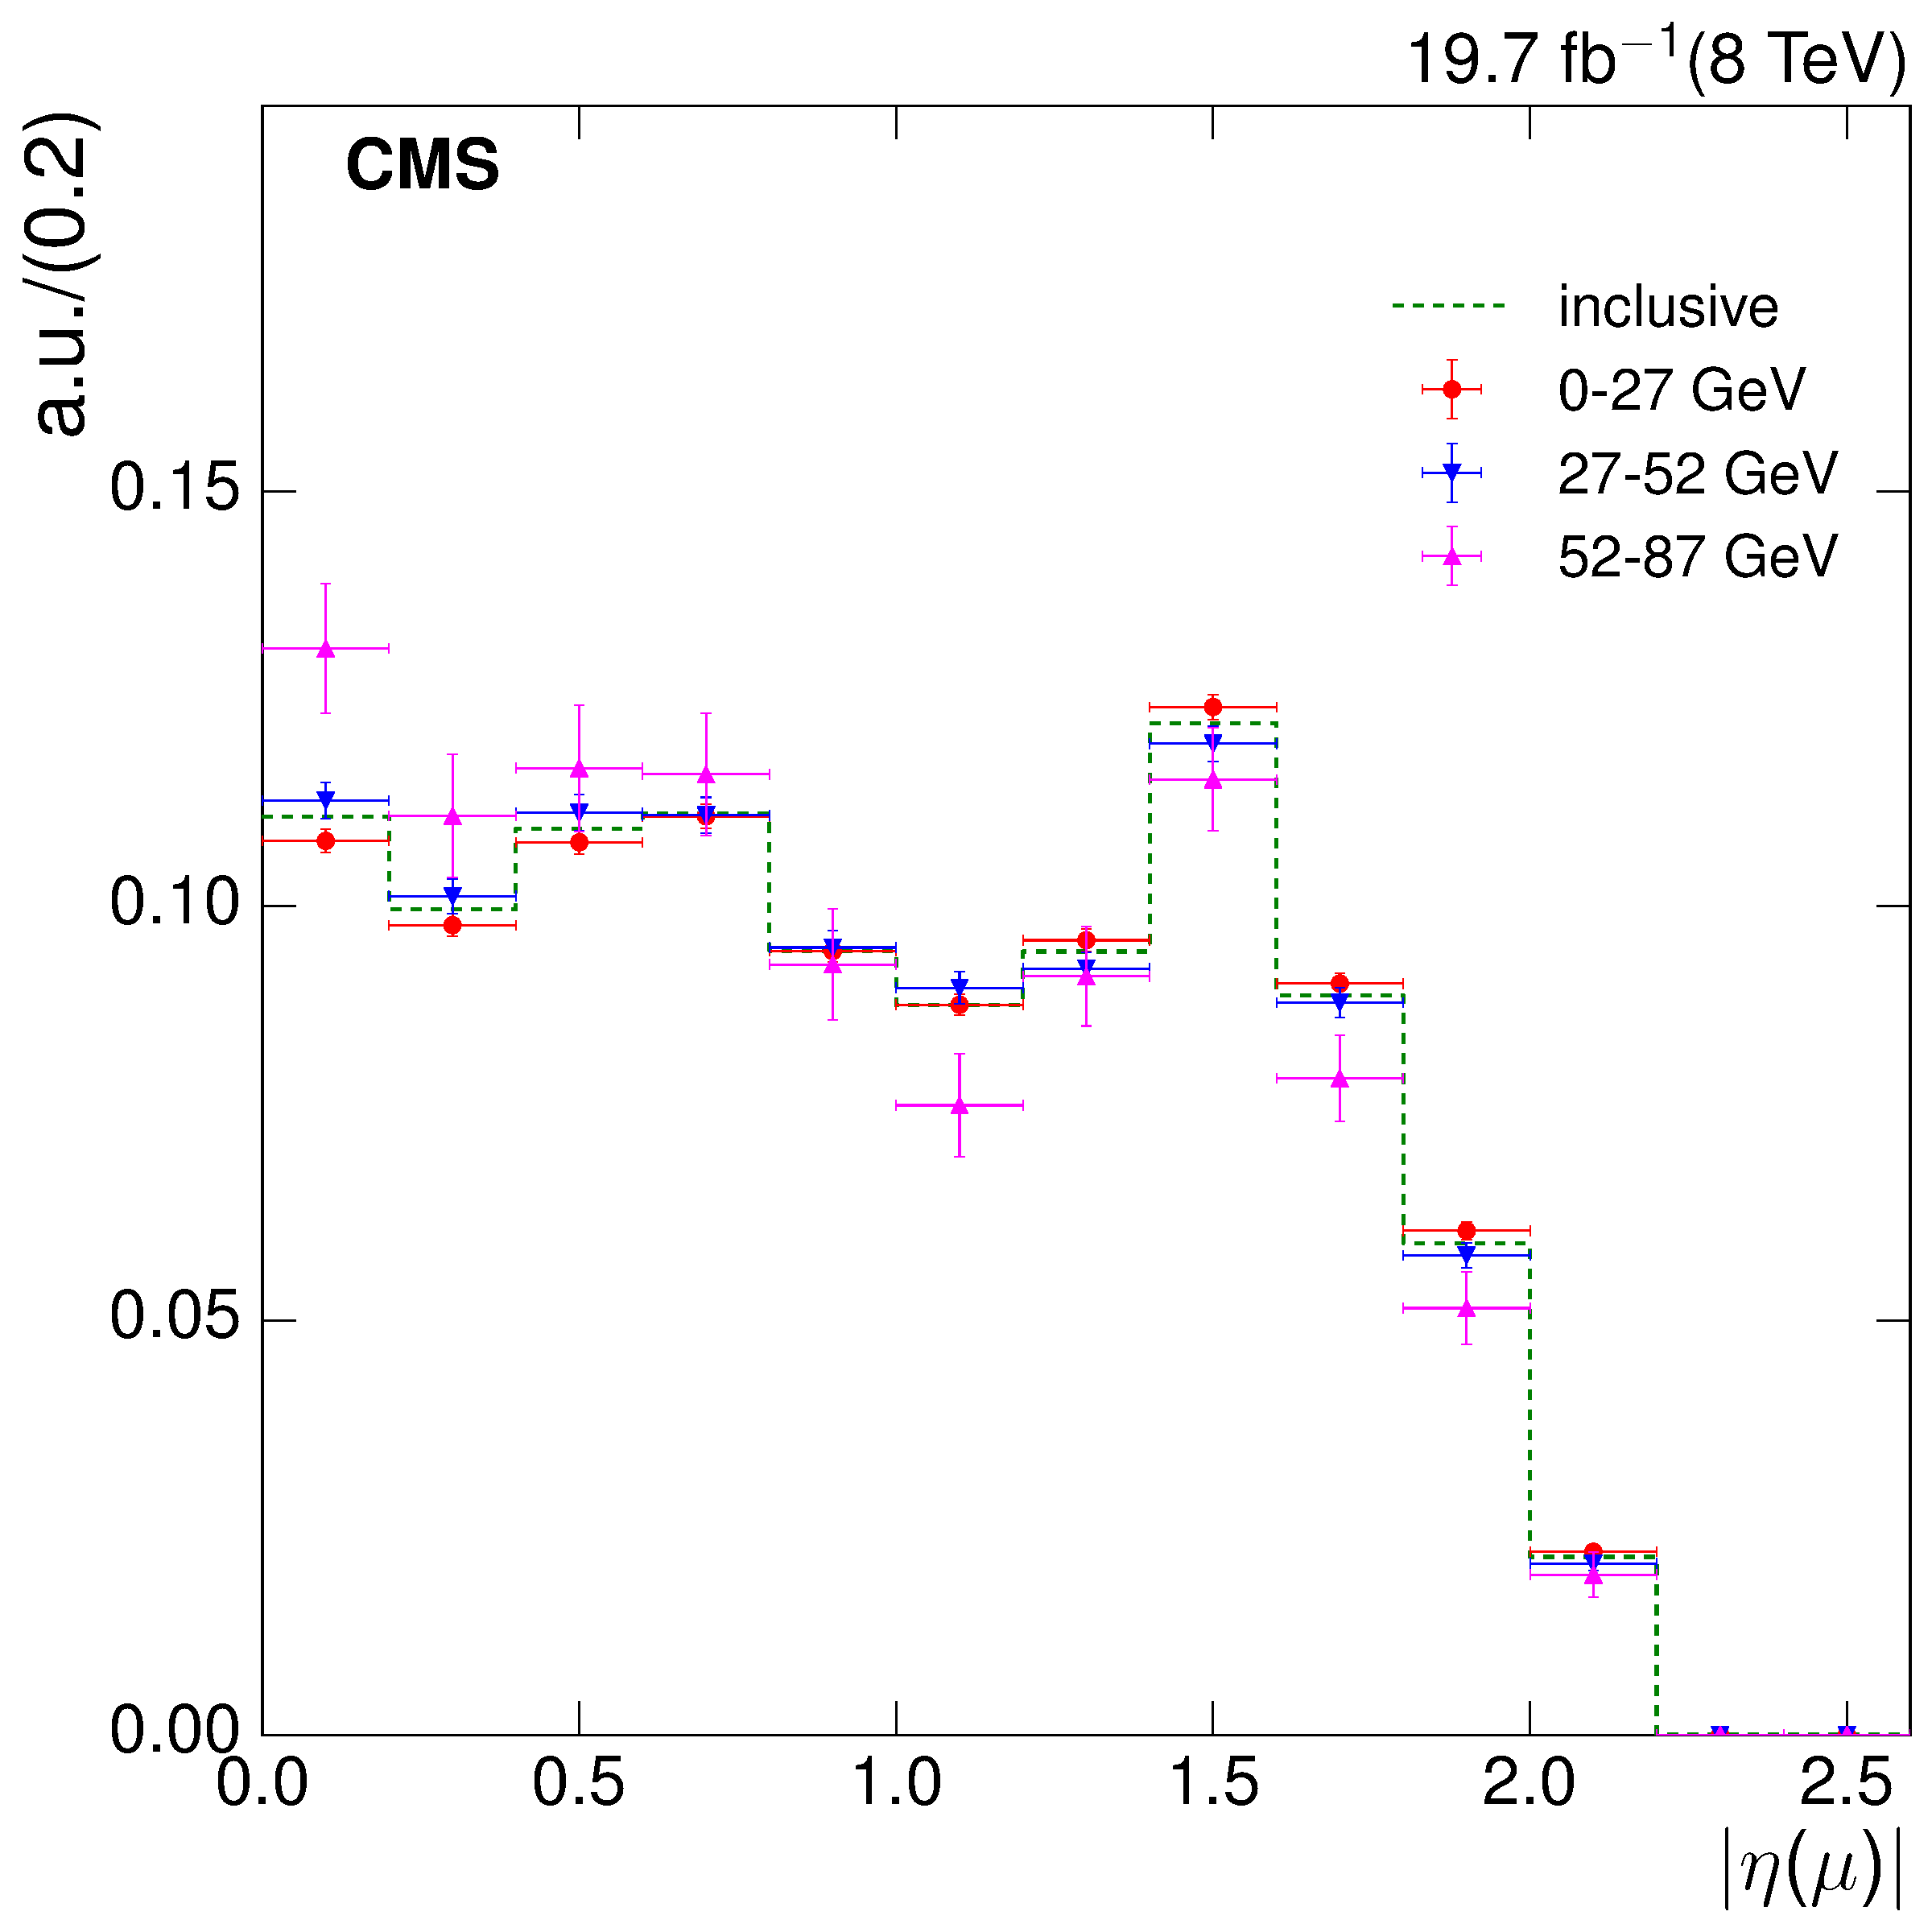
\includegraphics[width=0.48\textwidth]{Chapters/04_Analysis/04b_XSections/images/8TeV/fit_variables/muon/MET/muon_absolute_eta/qcd/MET_muon_absolute_eta_0orMoreBtag_QCD_template_comparison.pdf}\hfill
     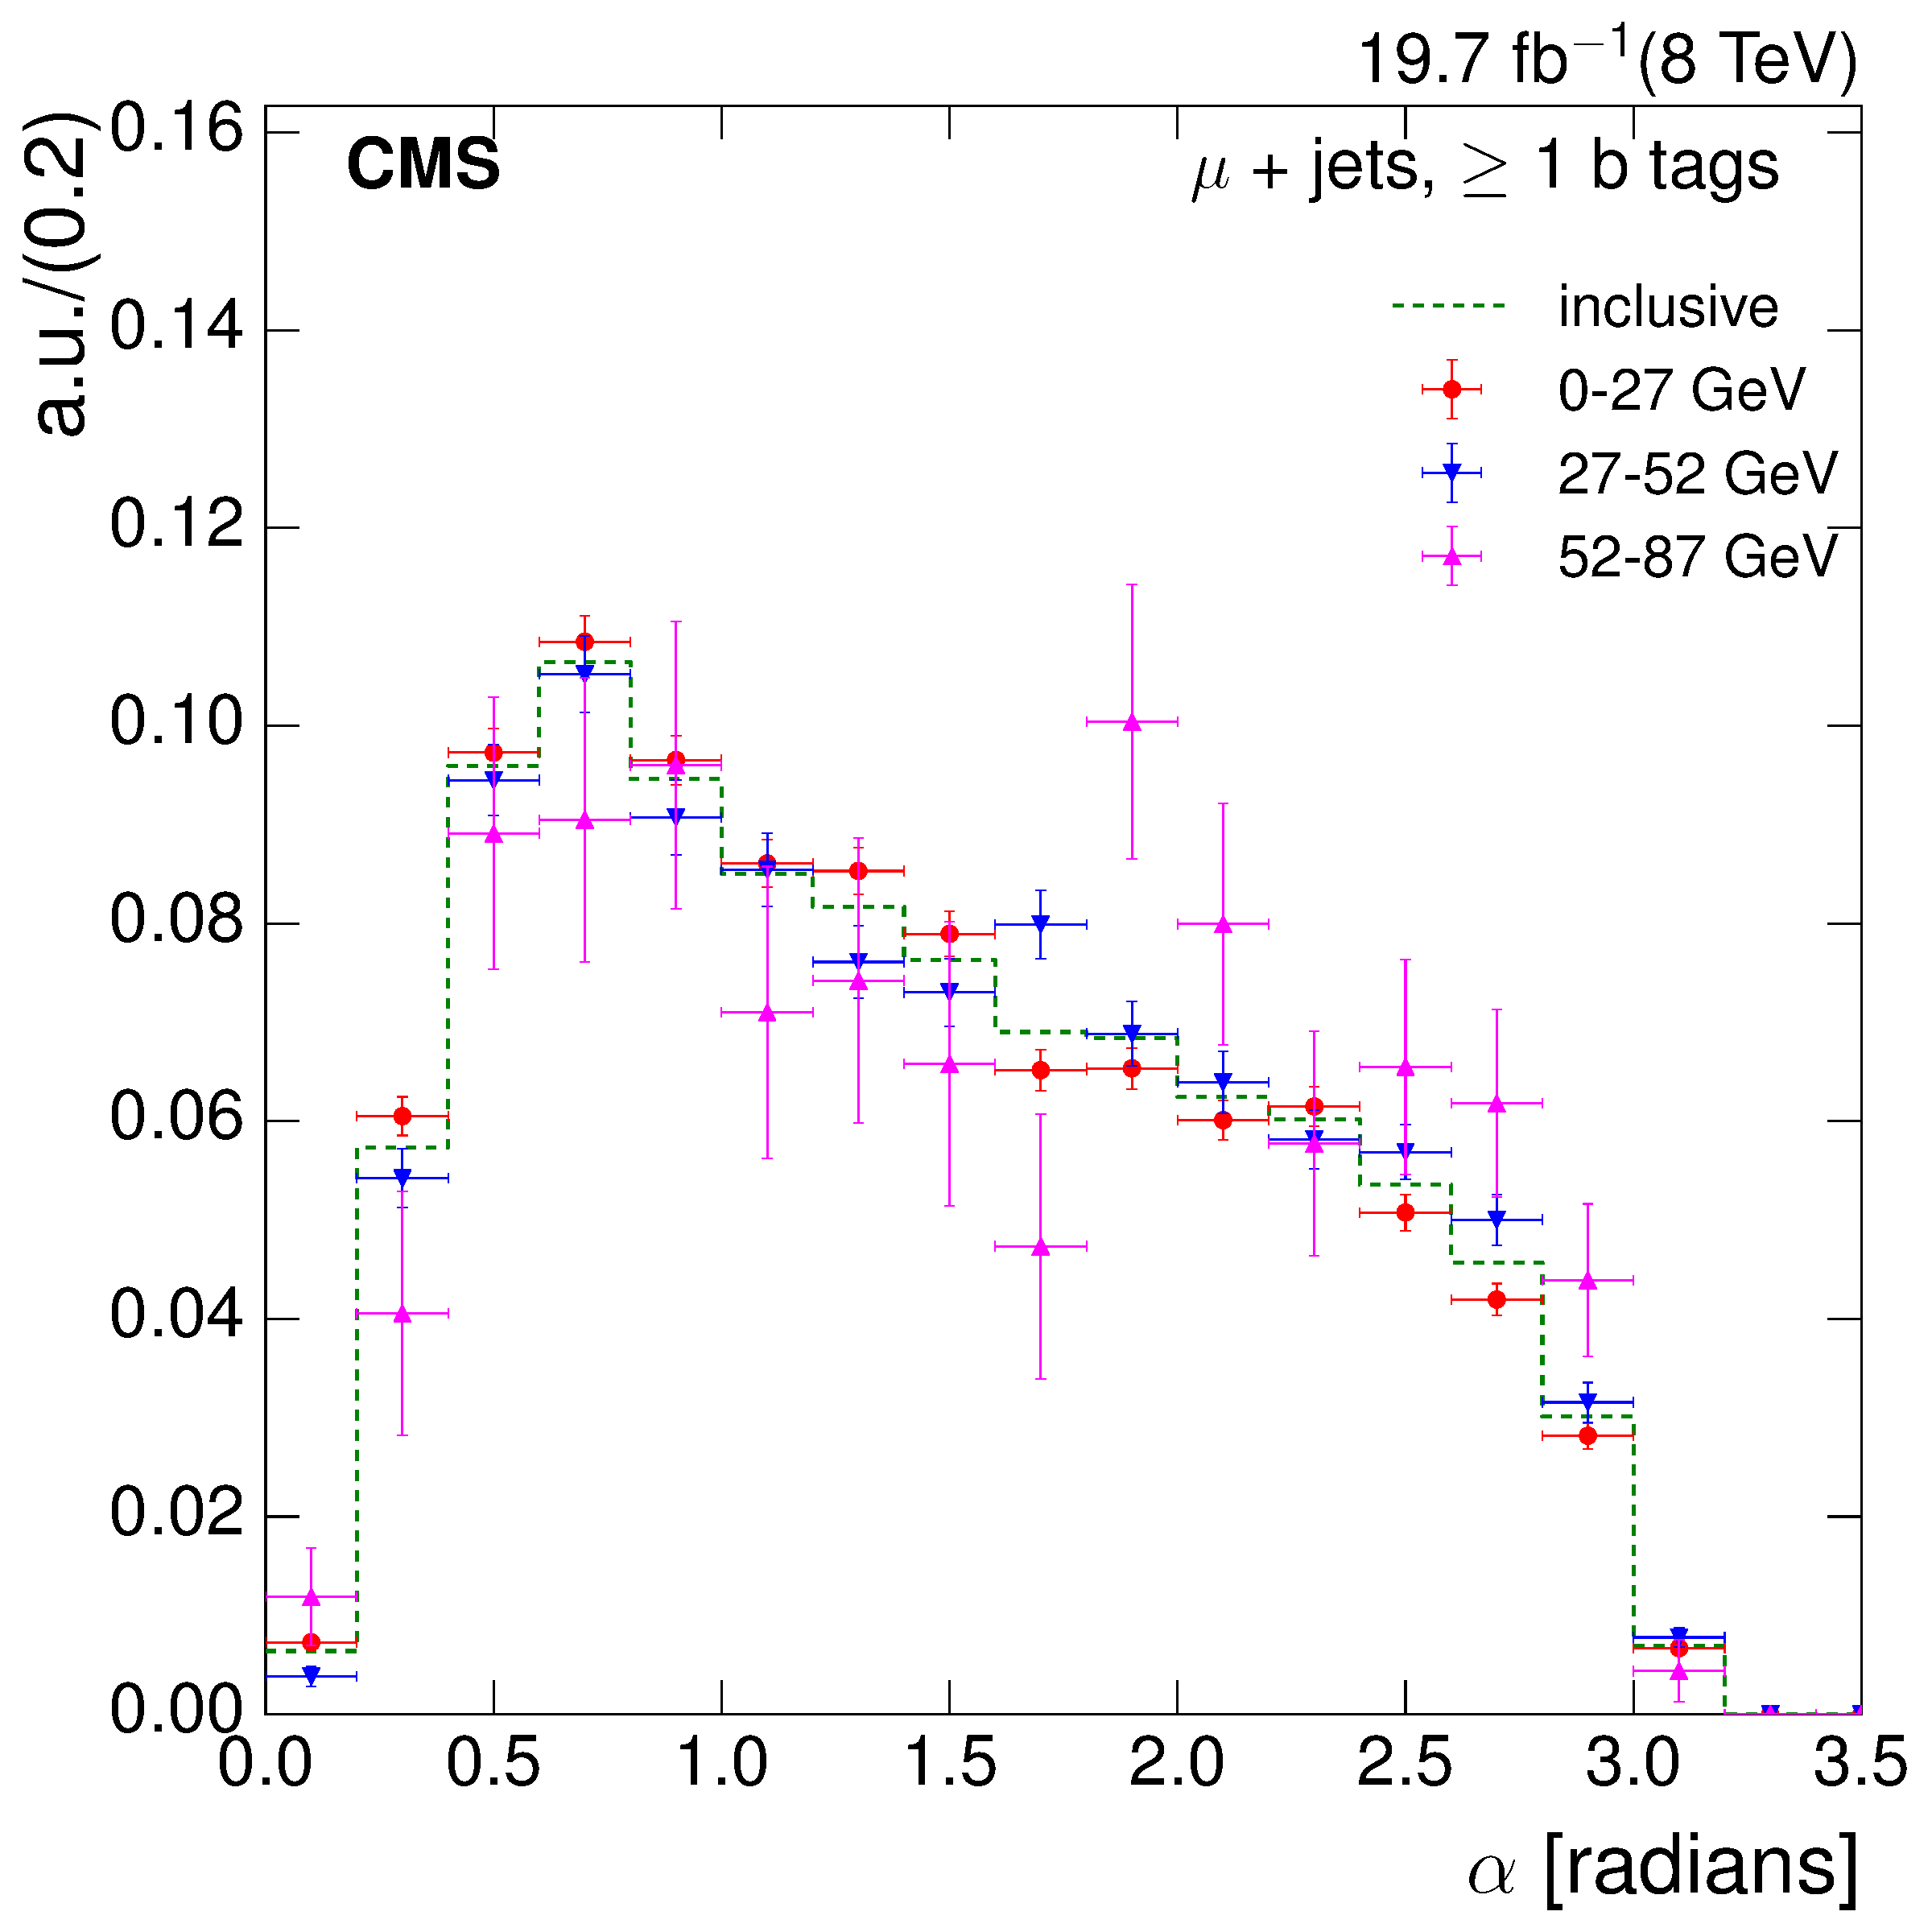
\includegraphics[width=0.48\textwidth]{Chapters/04_Analysis/04b_XSections/images/8TeV/fit_variables/muon/MET/angle_bl/qcd/MET_angle_bl_1orMoreBtag_QCD_template_comparison.pdf}\\
     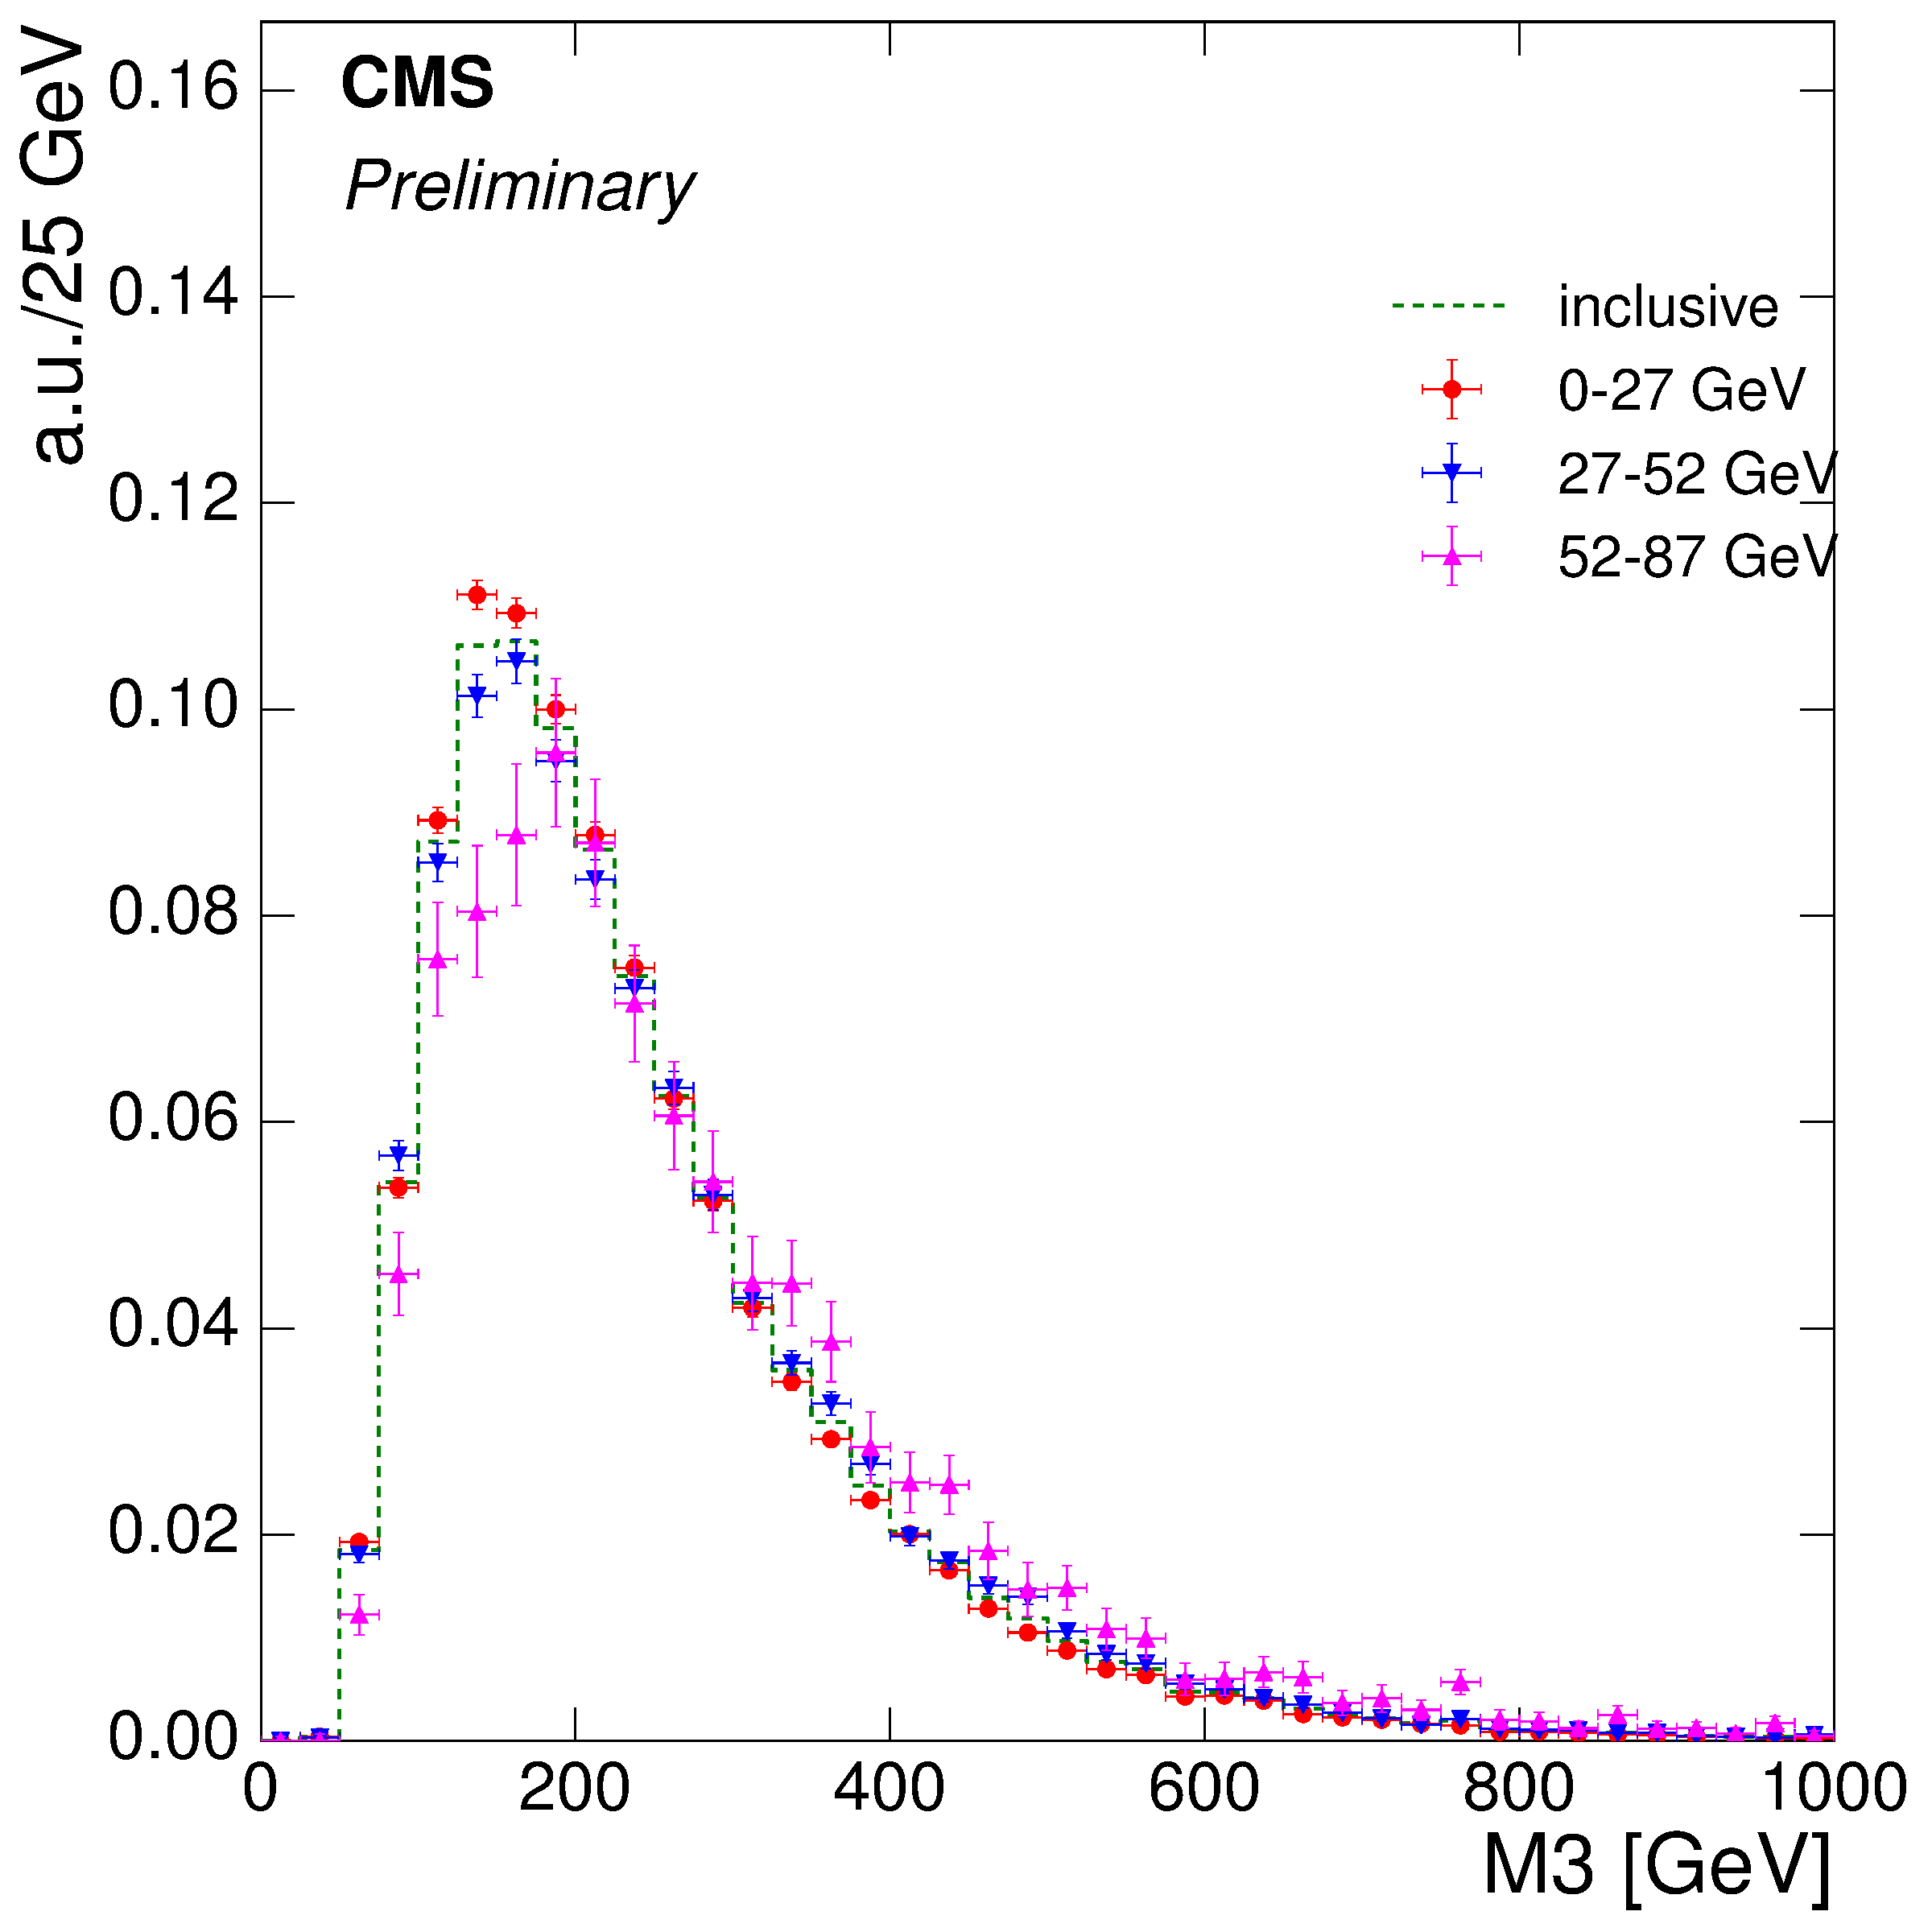
\includegraphics[width=0.48\textwidth]{Chapters/04_Analysis/04b_XSections/images/8TeV/fit_variables/muon/MET/M3/qcd/MET_M3_0orMoreBtag_QCD_template_comparison.pdf}\\
	 \caption{Normalised distributions of the QCD templates for the three fit variables at $\sqrt{s}=8\TeV$
	 inclusive across all \met bins and for the lowest three \met bins in the muon+jets channel: muon
	 \abseta (upper left), $\alpha$ (upper right) and M3 (lower).}
     \label{fig:MET_fit_variable_qcd_comparisons_muon_8TeV}
\end{figure}

\begin{figure}[hbtp]
    \centering
     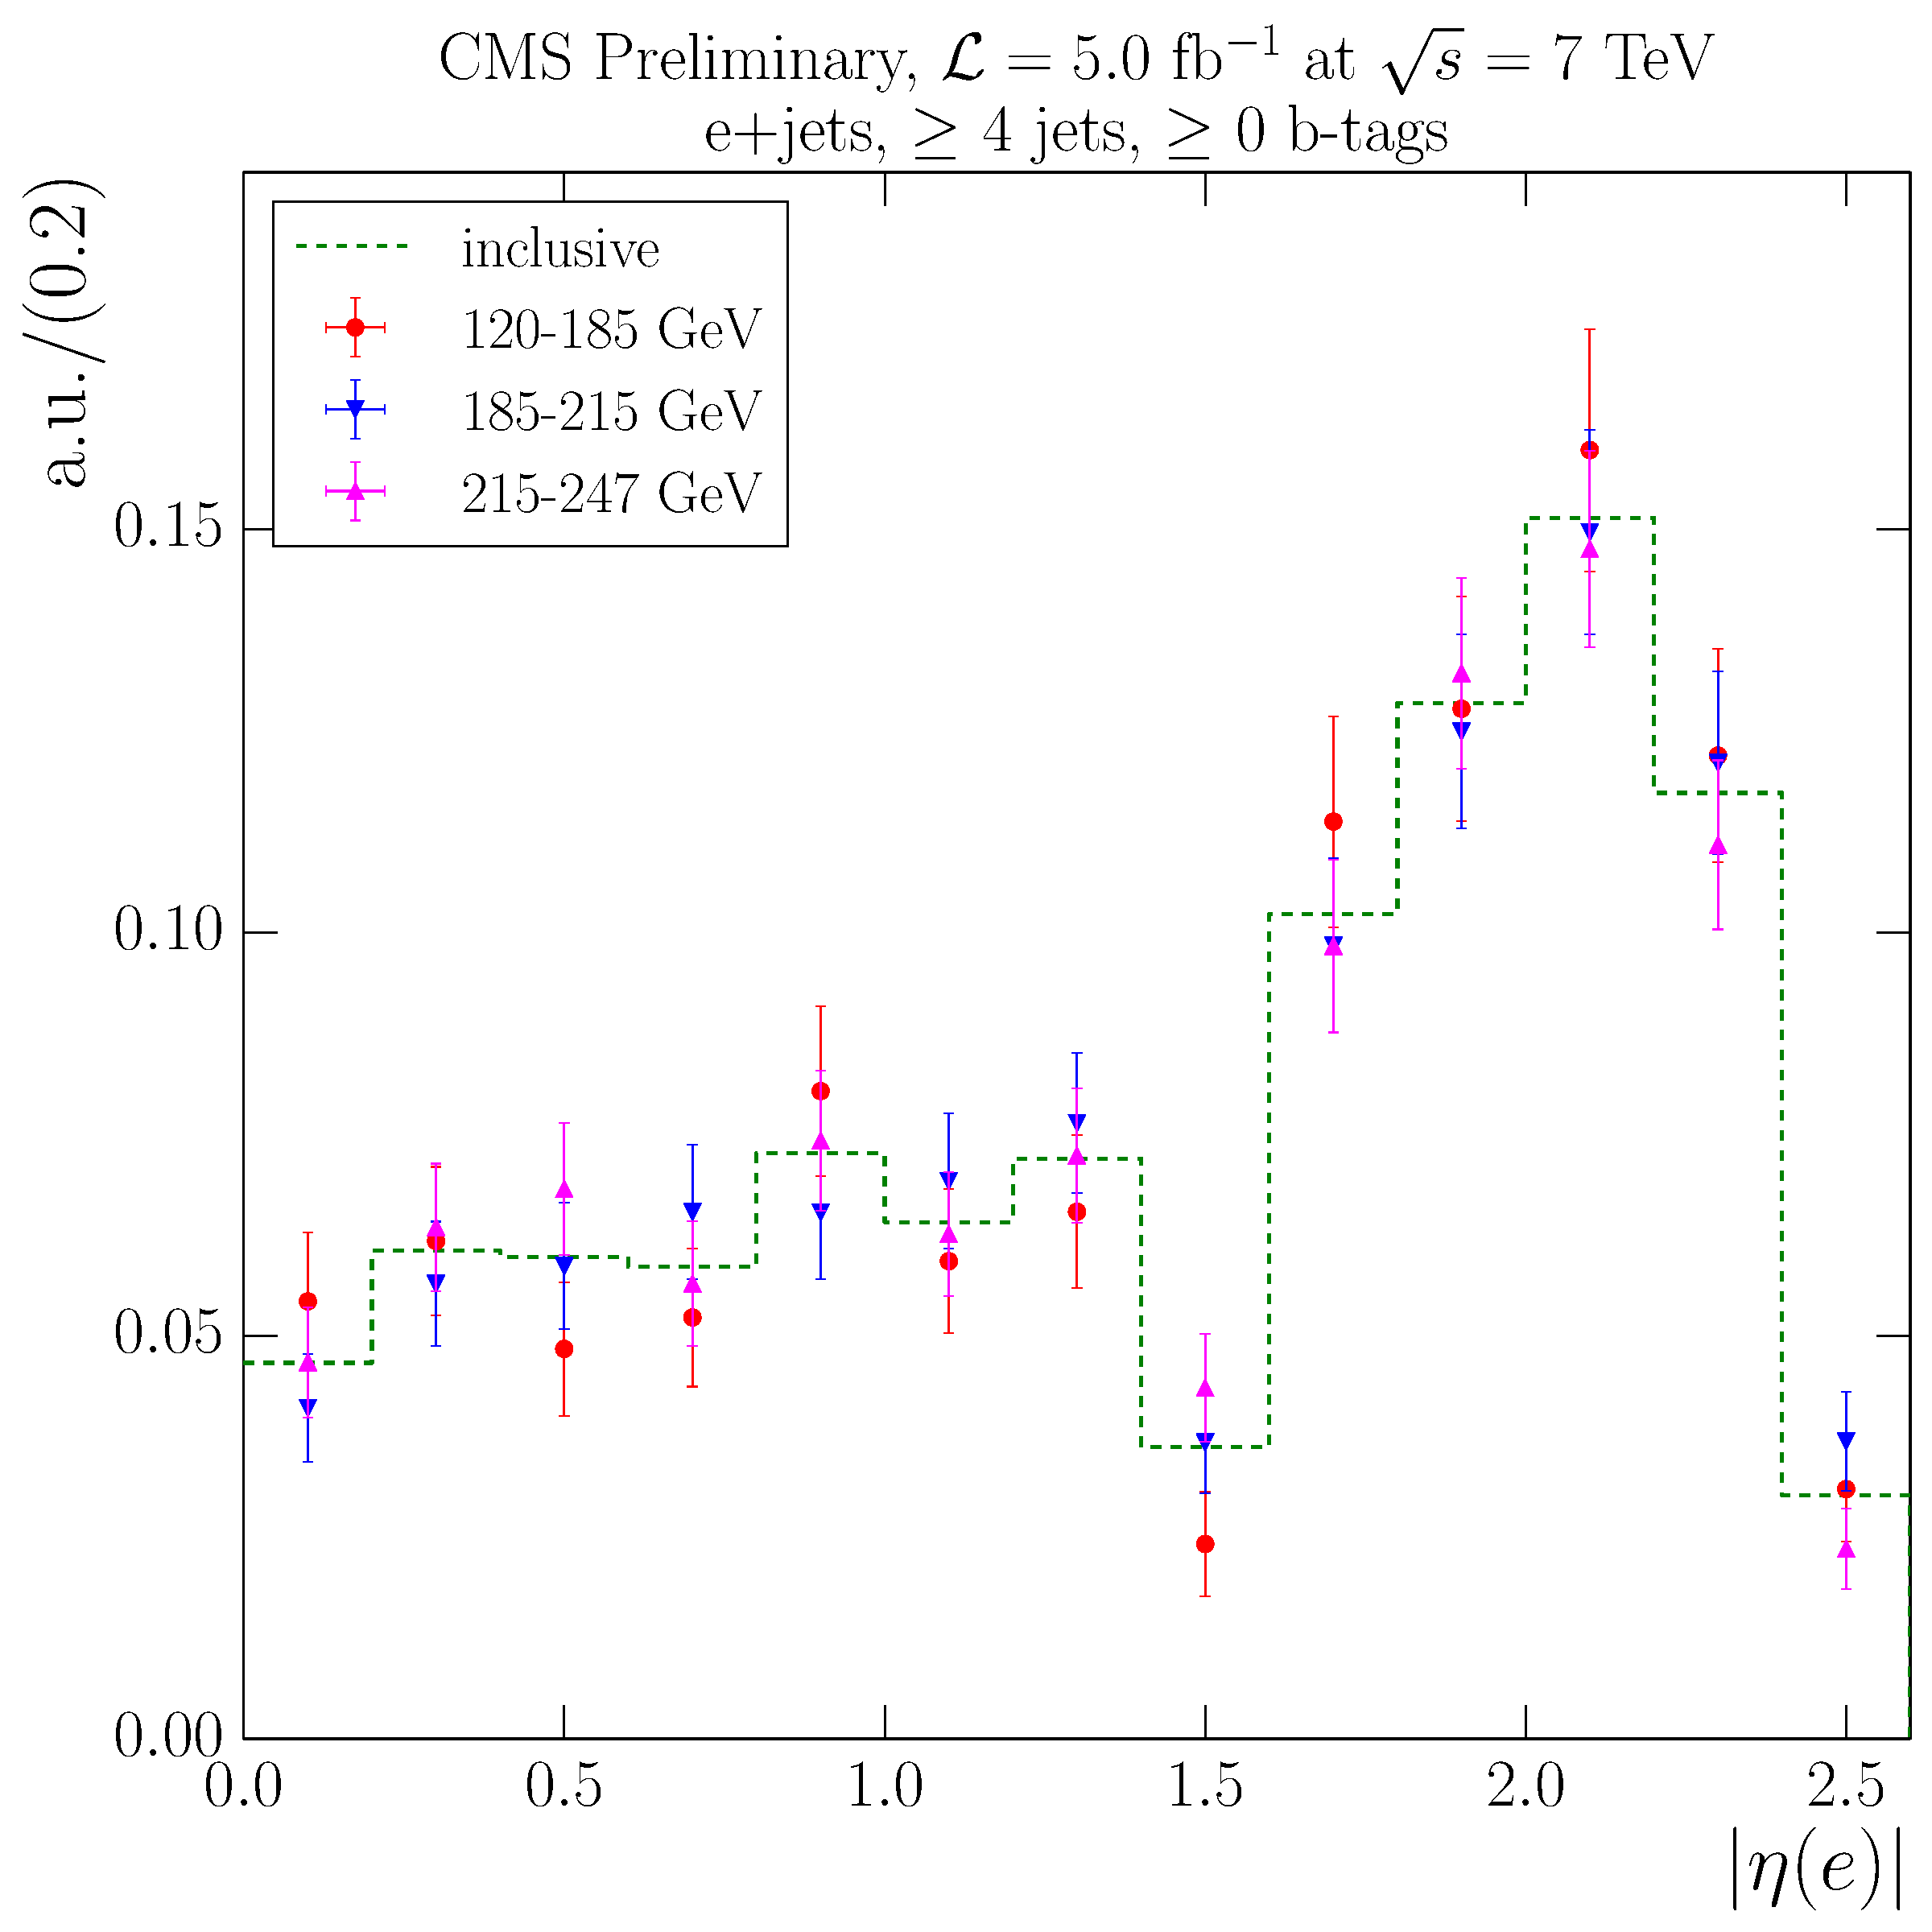
\includegraphics[width=0.48\textwidth]{Chapters/04_Analysis/04b_XSections/images/8TeV/fit_variables/electron/HT/electron_absolute_eta/qcd/HT_electron_absolute_eta_0orMoreBtag_QCD_template_comparison.pdf}\hfill
     \includegraphics[width=0.48\textwidth]{Chapters/04_Analysis/04b_XSections/images/8TeV/fit_variables/electron/HT/angle_bl/qcd/HT_angle_bl_1orMoreBtag_QCD_template_comparison.pdf}\\
     \includegraphics[width=0.48\textwidth]{Chapters/04_Analysis/04b_XSections/images/8TeV/fit_variables/electron/HT/M3/qcd/HT_M3_0orMoreBtag_QCD_template_comparison.pdf}\\
	 \caption{Normalised distributions of the QCD templates for the three fit variables at $\sqrt{s}=8\TeV$
	 inclusive across all \HT bins and for the lowest three \HT bins in the electron+jets channel: electron
	 \abseta (upper left), $\alpha$ (upper right) and M3 (lower right).}
     \label{fig:HT_fit_variable_qcd_comparisons_electron_8TeV}
\end{figure}

\begin{figure}[hbtp]
    \centering
     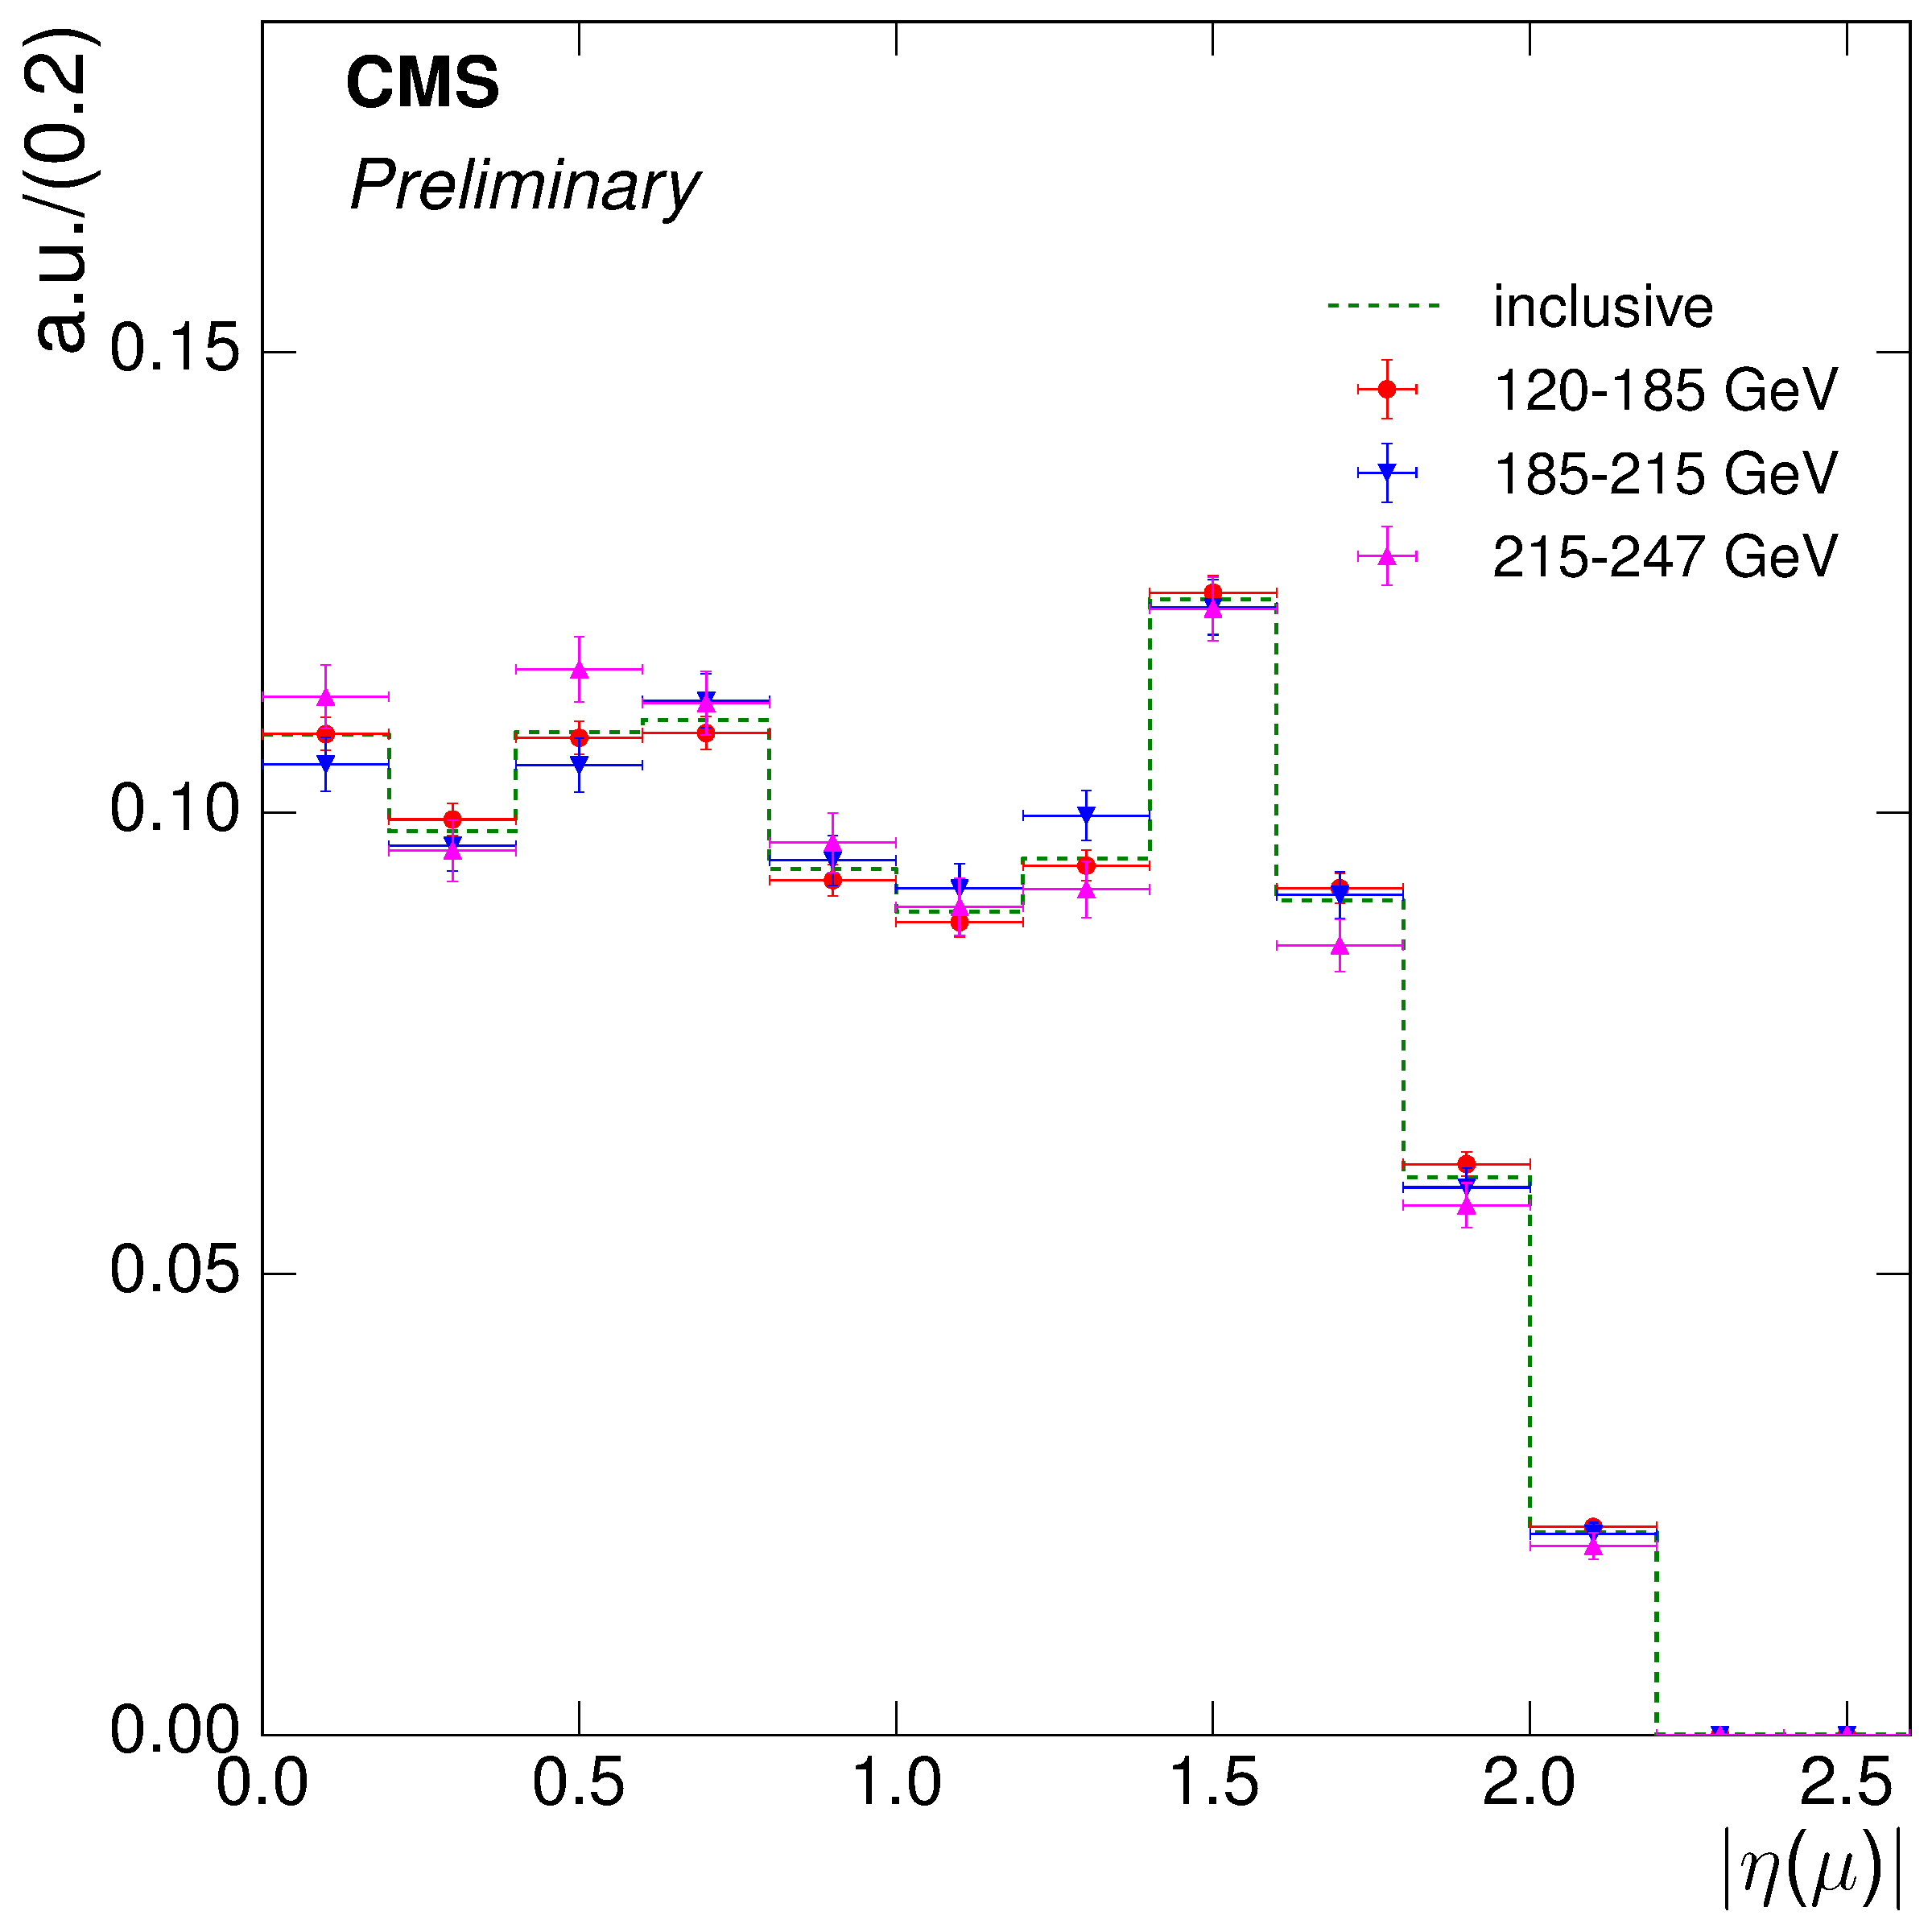
\includegraphics[width=0.48\textwidth]{Chapters/04_Analysis/04b_XSections/images/8TeV/fit_variables/muon/HT/muon_absolute_eta/qcd/HT_muon_absolute_eta_0orMoreBtag_QCD_template_comparison.pdf}\hfill
     \includegraphics[width=0.48\textwidth]{Chapters/04_Analysis/04b_XSections/images/8TeV/fit_variables/muon/HT/angle_bl/qcd/HT_angle_bl_1orMoreBtag_QCD_template_comparison.pdf}\\
     \includegraphics[width=0.48\textwidth]{Chapters/04_Analysis/04b_XSections/images/8TeV/fit_variables/muon/HT/M3/qcd/HT_M3_0orMoreBtag_QCD_template_comparison.pdf}\\
	 \caption{Normalised distributions of the QCD templates for the three fit variables at $\sqrt{s}=8\TeV$
	 inclusive across all \HT bins and for the lowest three \HT bins in the muon+jets channel: muon \abseta
	 (upper left), $\alpha$ (upper right) and M3 (lower right).}
     \label{fig:HT_fit_variable_qcd_comparisons_muon_8TeV}
\end{figure}

\begin{figure}[hbtp]
    \centering
     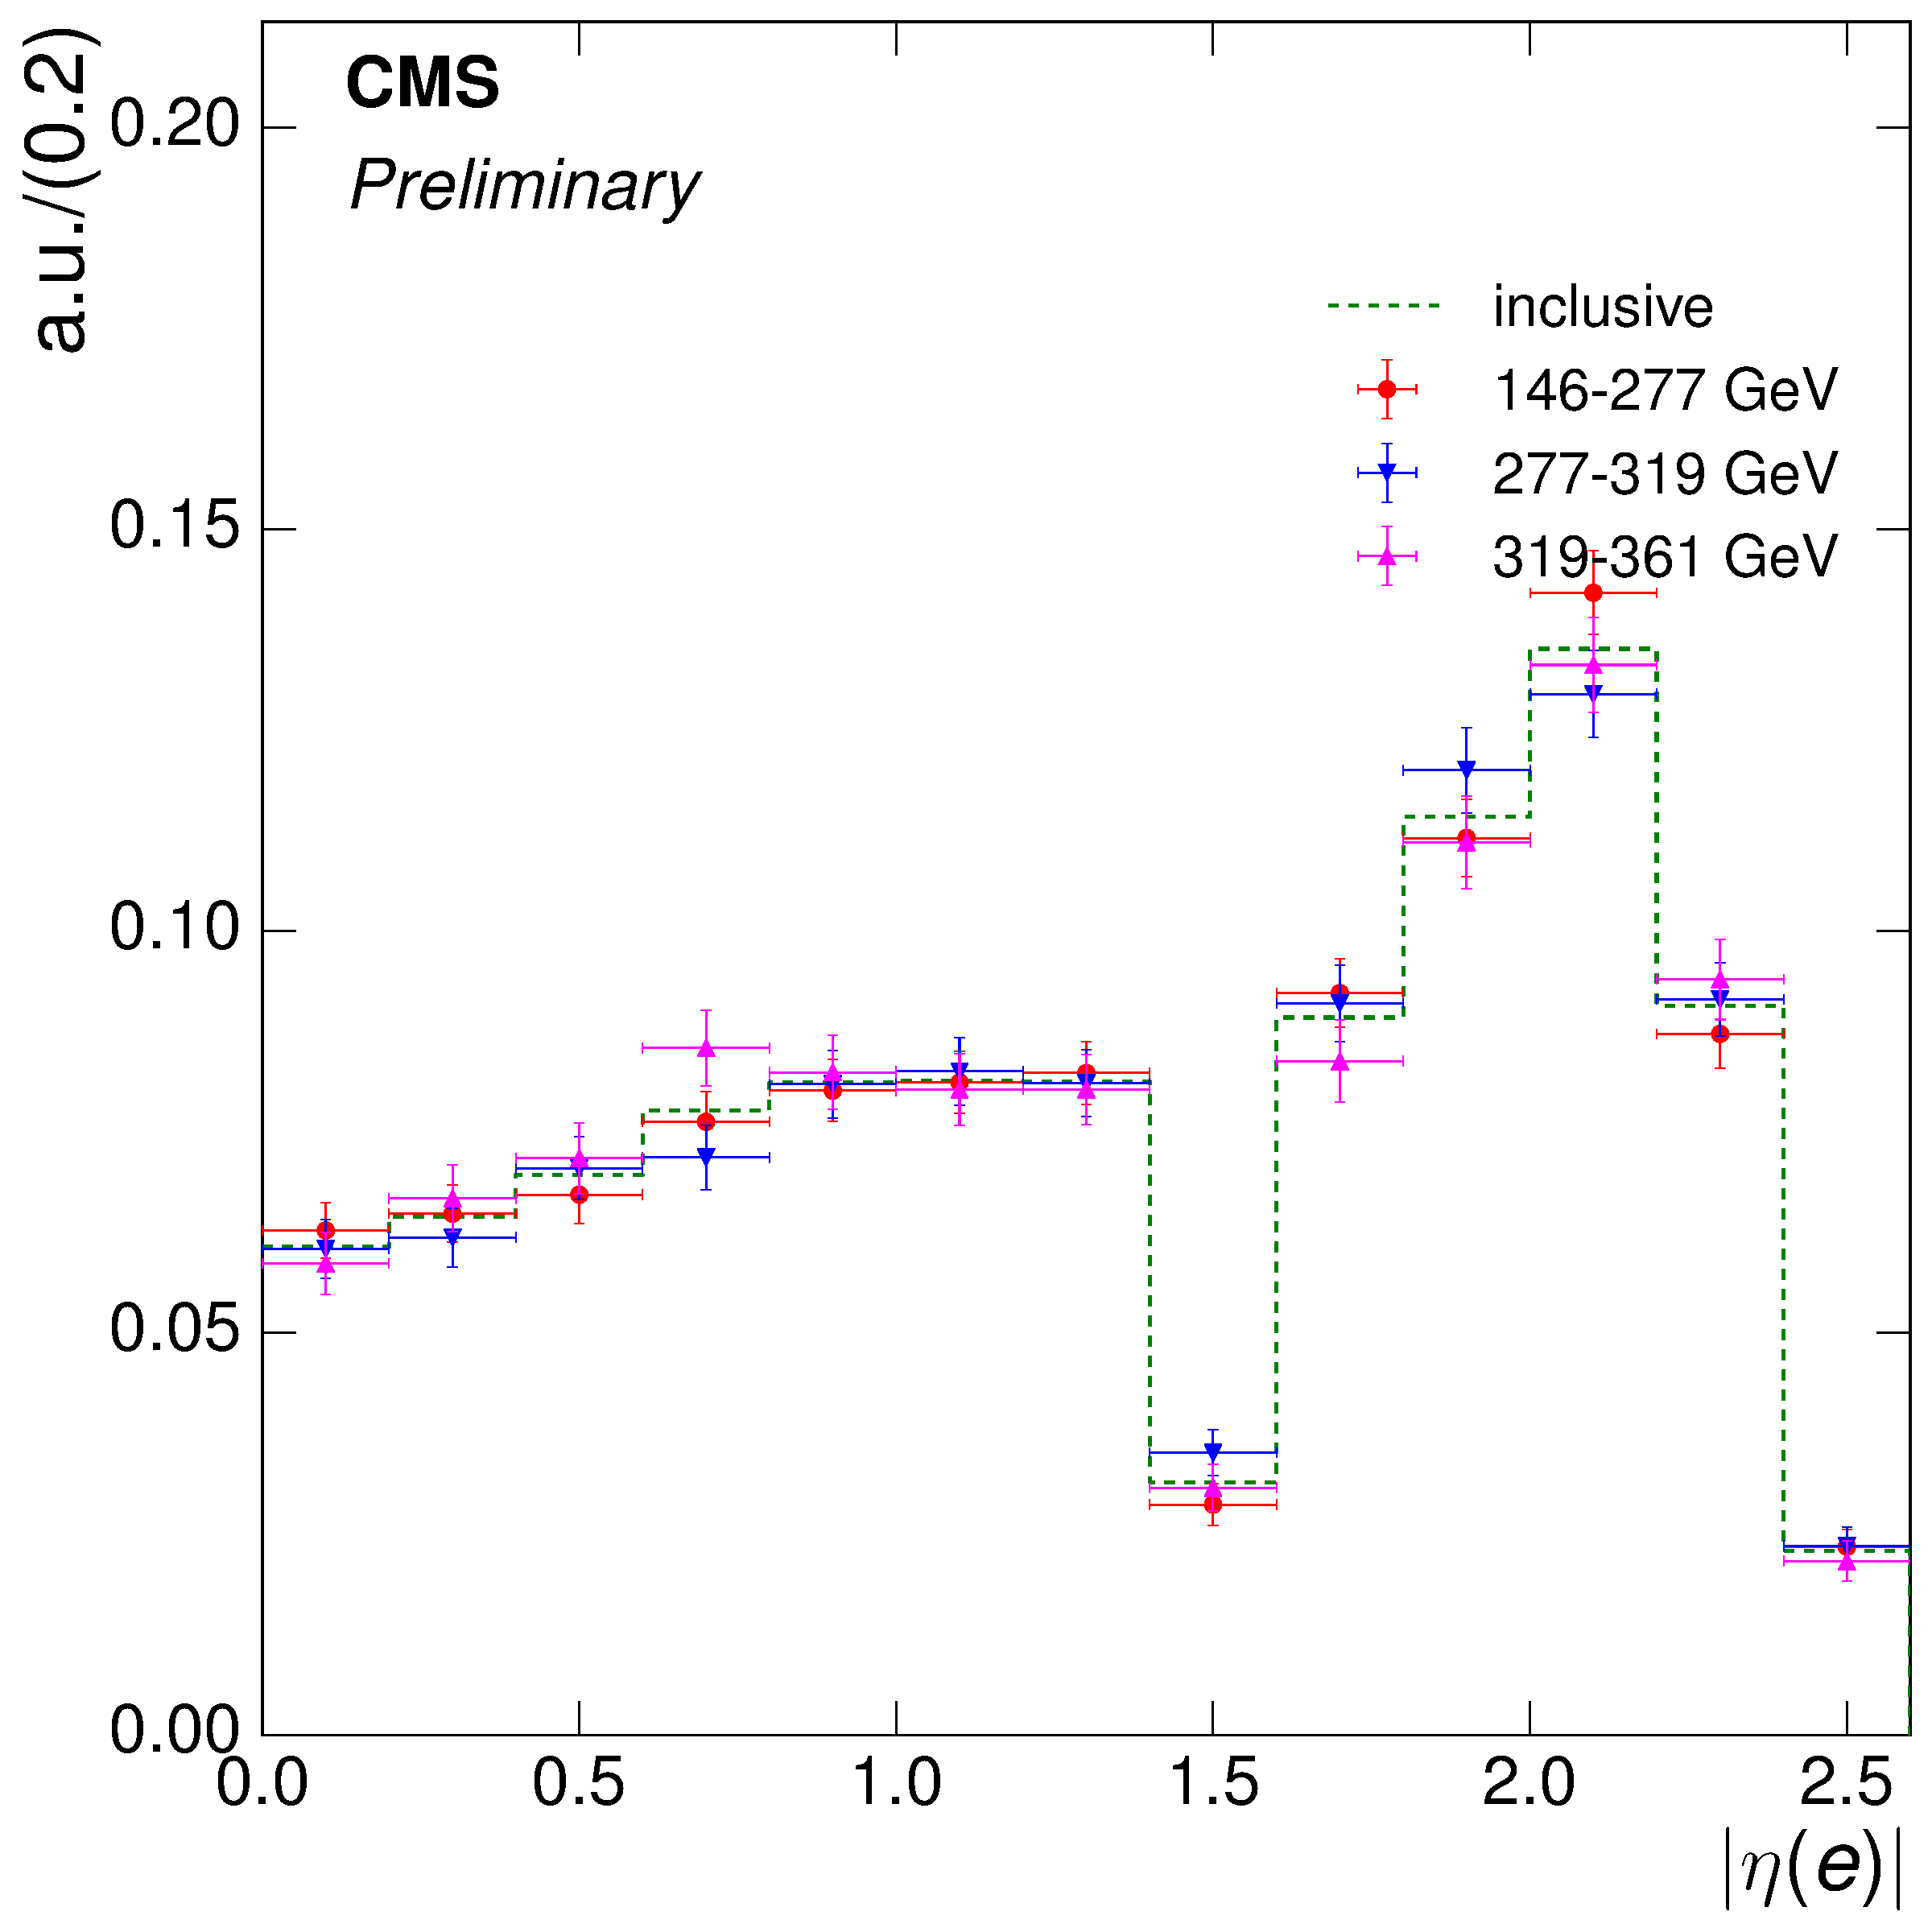
\includegraphics[width=0.48\textwidth]{Chapters/04_Analysis/04b_XSections/images/8TeV/fit_variables/electron/ST/electron_absolute_eta/qcd/ST_electron_absolute_eta_0orMoreBtag_QCD_template_comparison.pdf}\hfill
     \includegraphics[width=0.48\textwidth]{Chapters/04_Analysis/04b_XSections/images/8TeV/fit_variables/electron/ST/angle_bl/qcd/ST_angle_bl_1orMoreBtag_QCD_template_comparison.pdf}\\
     \includegraphics[width=0.48\textwidth]{Chapters/04_Analysis/04b_XSections/images/8TeV/fit_variables/electron/ST/M3/qcd/ST_M3_0orMoreBtag_QCD_template_comparison.pdf}\\
	 \caption{Normalised distributions of the QCD templates for the three fit variables at $\sqrt{s}=8\TeV$
	 inclusive across all \st bins and for the lowest three \st bins in the electron+jets channel: electron
	 \abseta (upper left), $\alpha$ (upper right) and M3 (lower right).}
     \label{fig:ST_fit_variable_qcd_comparisons_electron_8TeV}
\end{figure}

\begin{figure}[hbtp]
    \centering
     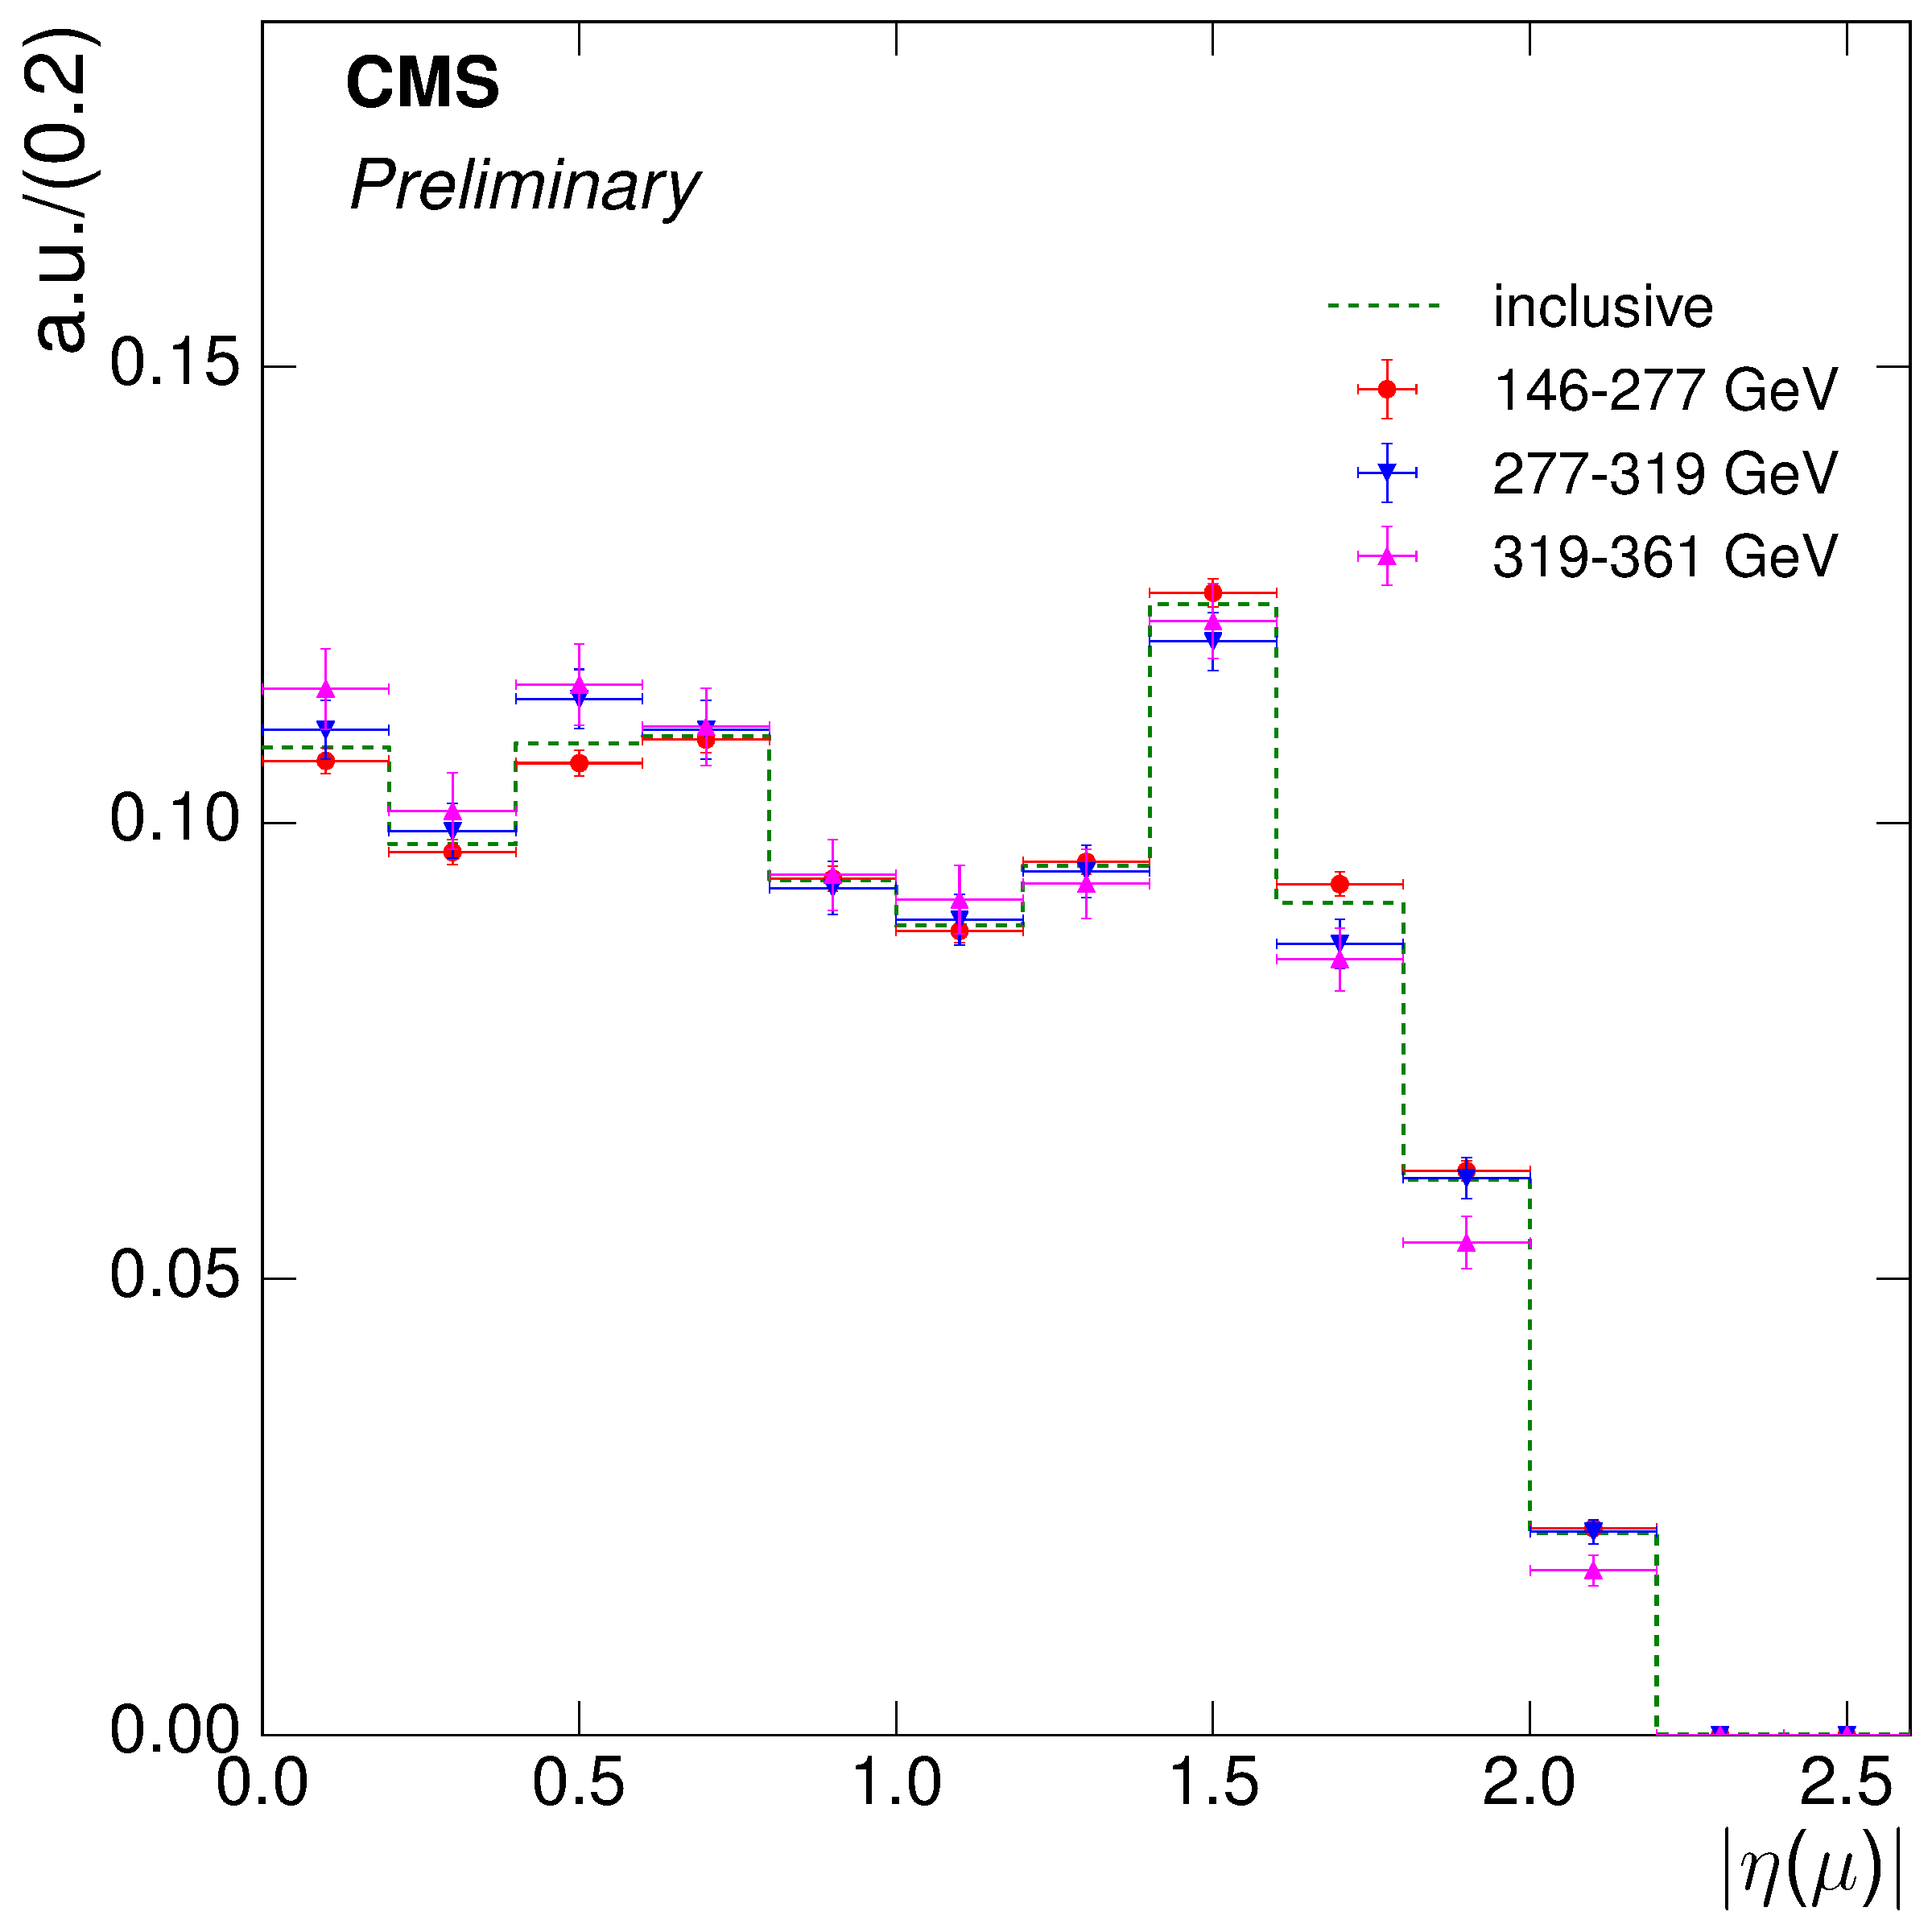
\includegraphics[width=0.48\textwidth]{Chapters/04_Analysis/04b_XSections/images/8TeV/fit_variables/muon/ST/muon_absolute_eta/qcd/ST_muon_absolute_eta_0orMoreBtag_QCD_template_comparison.pdf}\hfill
     \includegraphics[width=0.48\textwidth]{Chapters/04_Analysis/04b_XSections/images/8TeV/fit_variables/muon/ST/angle_bl/qcd/ST_angle_bl_1orMoreBtag_QCD_template_comparison.pdf}\\
     \includegraphics[width=0.48\textwidth]{Chapters/04_Analysis/04b_XSections/images/8TeV/fit_variables/muon/ST/M3/qcd/ST_M3_0orMoreBtag_QCD_template_comparison.pdf}\\
	 \caption{Normalised distributions of the QCD templates for the three fit variables at $\sqrt{s}=8\TeV$
	 inclusive across all \st bins and for the lowest three \st bins in the muon+jets channel: muon \abseta
	 (upper left), $\alpha$ (upper right) and M3 (lower right).}
     \label{fig:ST_fit_variable_qcd_comparisons_muon_8TeV}
\end{figure}


\begin{figure}[hbtp]
    \centering
     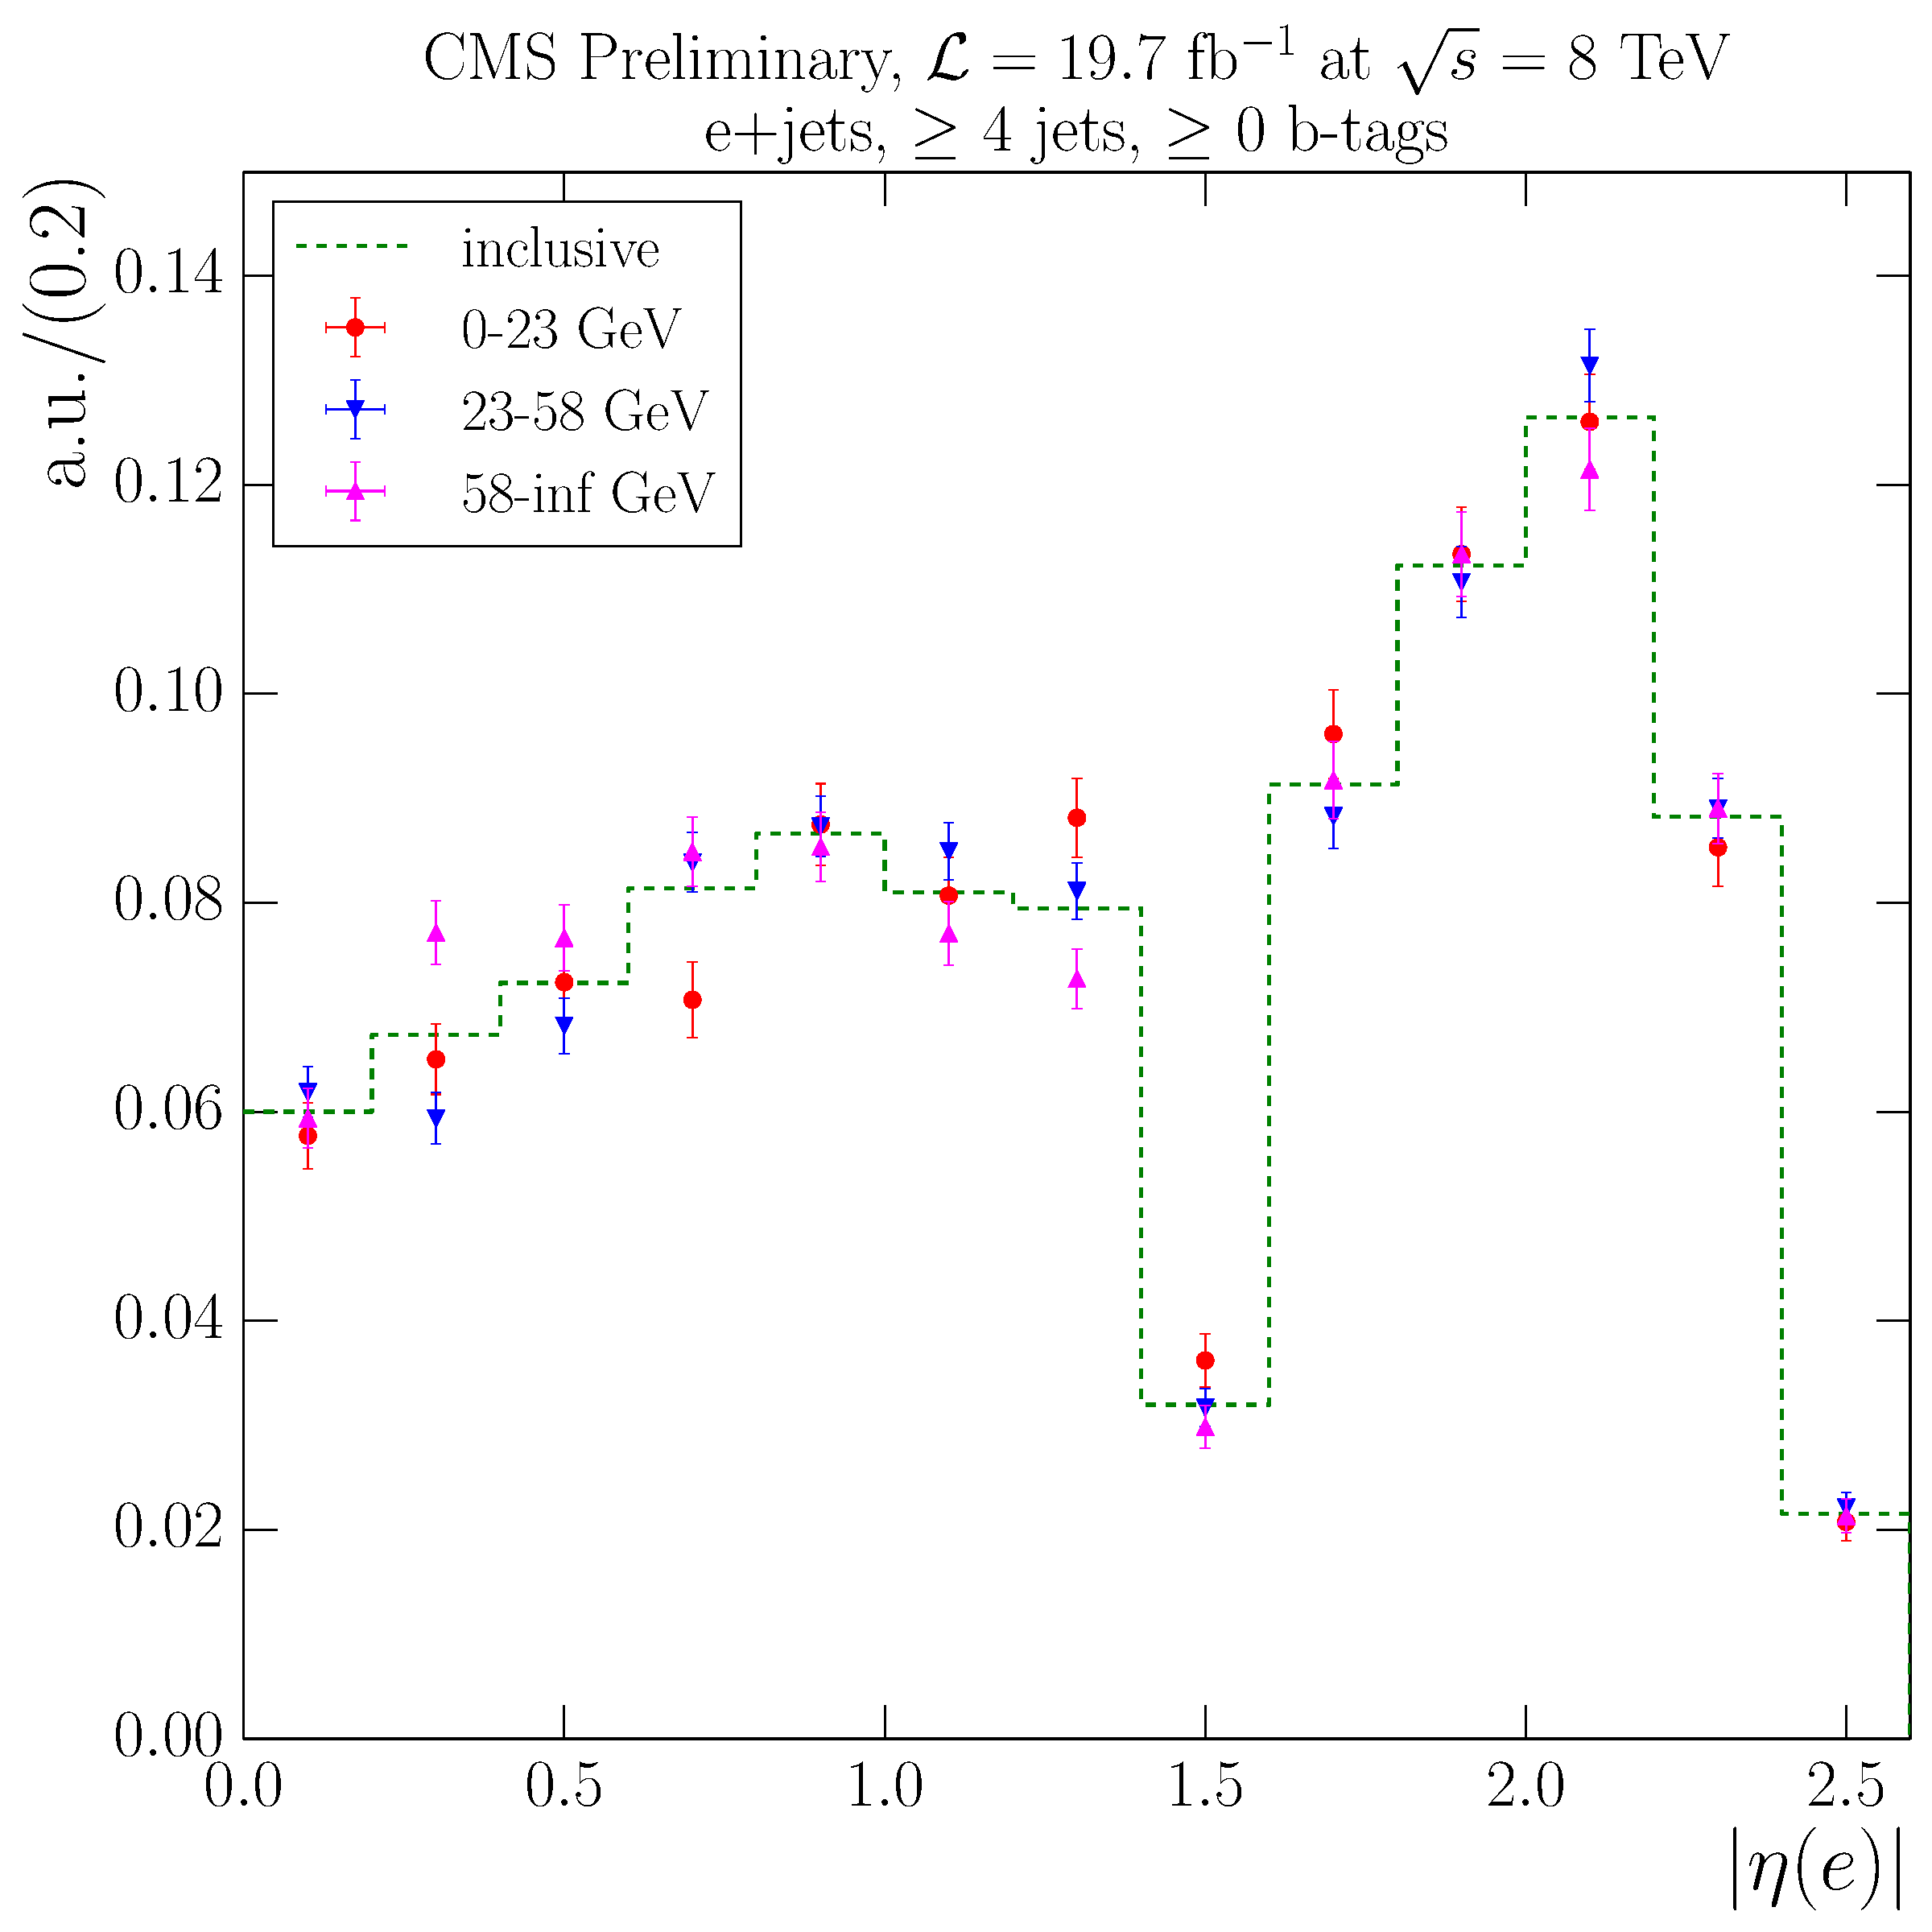
\includegraphics[width=0.48\textwidth]{Chapters/04_Analysis/04b_XSections/images/8TeV/fit_variables/electron/MT/electron_absolute_eta/qcd/MT_electron_absolute_eta_0orMoreBtag_QCD_template_comparison.pdf}\hfill
     \includegraphics[width=0.48\textwidth]{Chapters/04_Analysis/04b_XSections/images/8TeV/fit_variables/electron/MT/angle_bl/qcd/MT_angle_bl_1orMoreBtag_QCD_template_comparison.pdf}\\
     \includegraphics[width=0.48\textwidth]{Chapters/04_Analysis/04b_XSections/images/8TeV/fit_variables/electron/MT/M3/qcd/MT_M3_0orMoreBtag_QCD_template_comparison.pdf}\\
	 \caption{Normalised distributions of the QCD templates for the three fit variables at $\sqrt{s}=8\TeV$
	 inclusive across all \mt bins and for the lowest three \mt bins in the electron+jets channel: electron
	 \abseta (upper left), $\alpha$ (upper right) and M3 (lower right).}
     \label{fig:MT_fit_variable_qcd_comparisons_electron_8TeV}
\end{figure}

\begin{figure}[hbtp]
    \centering
     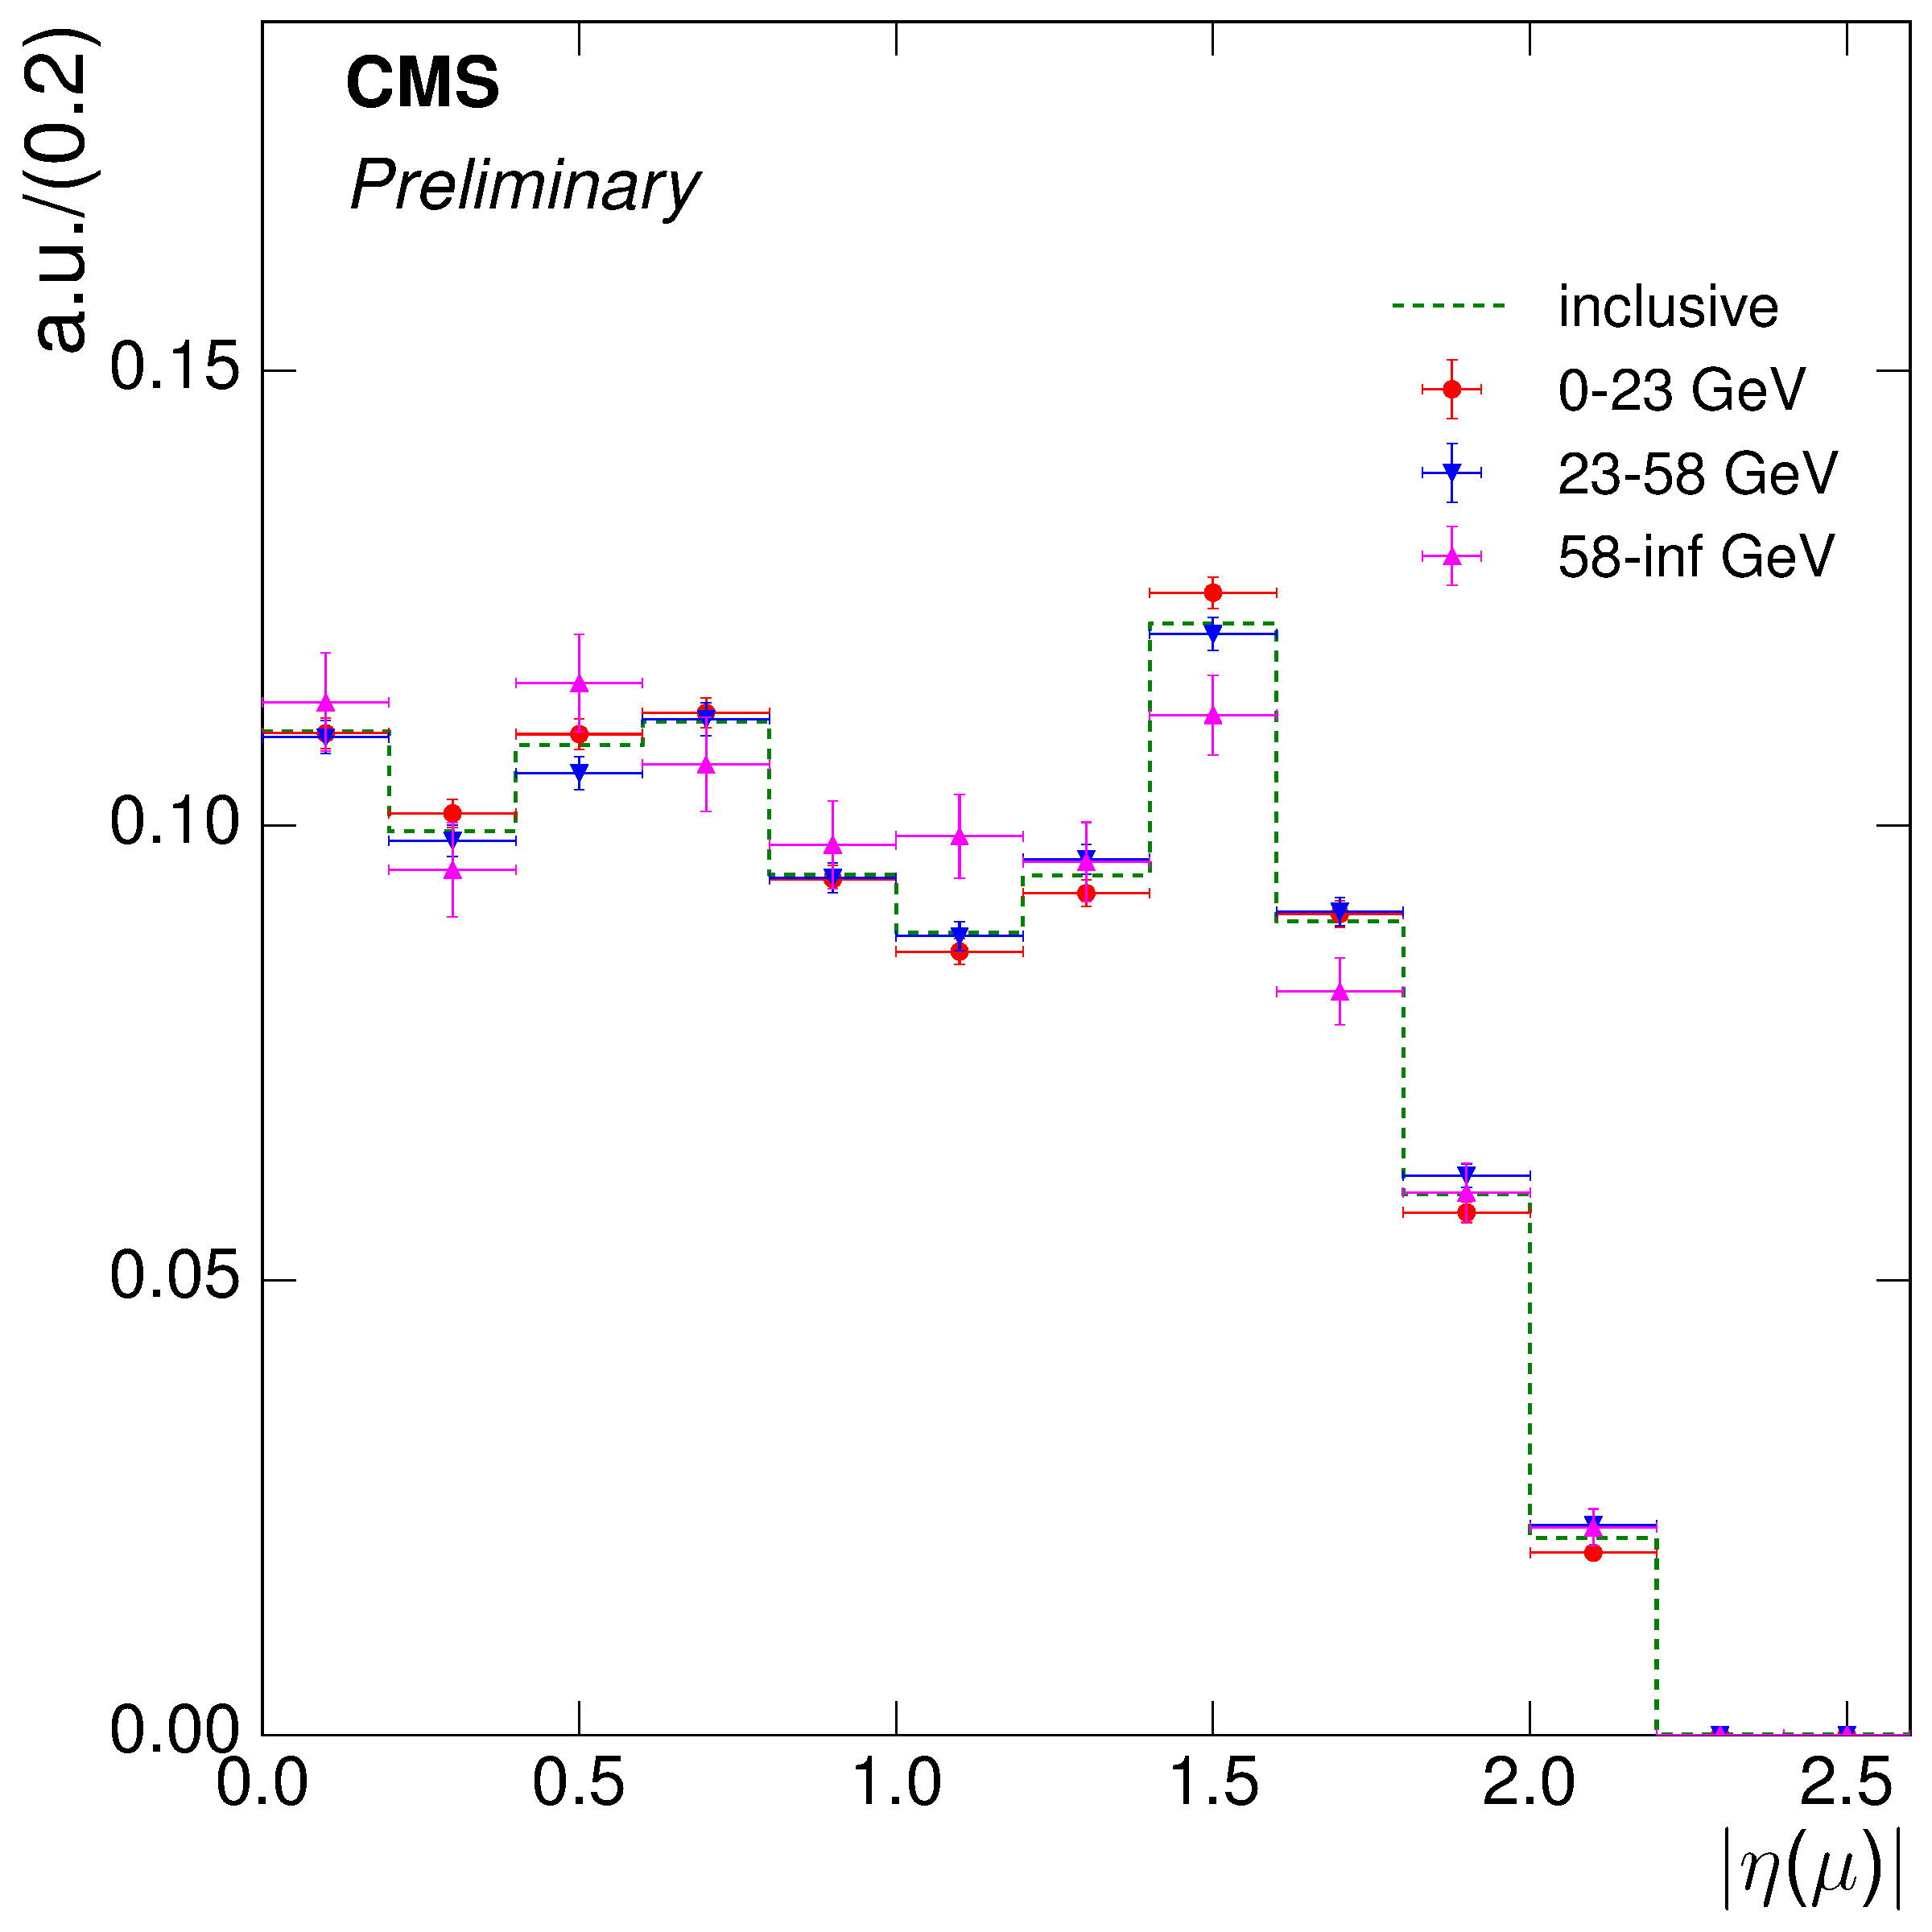
\includegraphics[width=0.48\textwidth]{Chapters/04_Analysis/04b_XSections/images/8TeV/fit_variables/muon/MT/muon_absolute_eta/qcd/MT_muon_absolute_eta_0orMoreBtag_QCD_template_comparison.pdf}\hfill
     \includegraphics[width=0.48\textwidth]{Chapters/04_Analysis/04b_XSections/images/8TeV/fit_variables/muon/MT/angle_bl/qcd/MT_angle_bl_1orMoreBtag_QCD_template_comparison.pdf}\\
     \includegraphics[width=0.48\textwidth]{Chapters/04_Analysis/04b_XSections/images/8TeV/fit_variables/muon/MT/M3/qcd/MT_M3_0orMoreBtag_QCD_template_comparison.pdf}\\
	 \caption{Normalised distributions of the QCD templates for the three fit variables at $\sqrt{s}=8\TeV$
	 inclusive across all \mt bins and for the lowest three \mt bins in the muon+jets channel: muon \abseta
	 (upper left), $\alpha$ (upper right) and M3 (lower right).}
     \label{fig:MT_fit_variable_qcd_comparisons_muon_8TeV}
\end{figure}

\begin{figure}[hbtp]
    \centering
     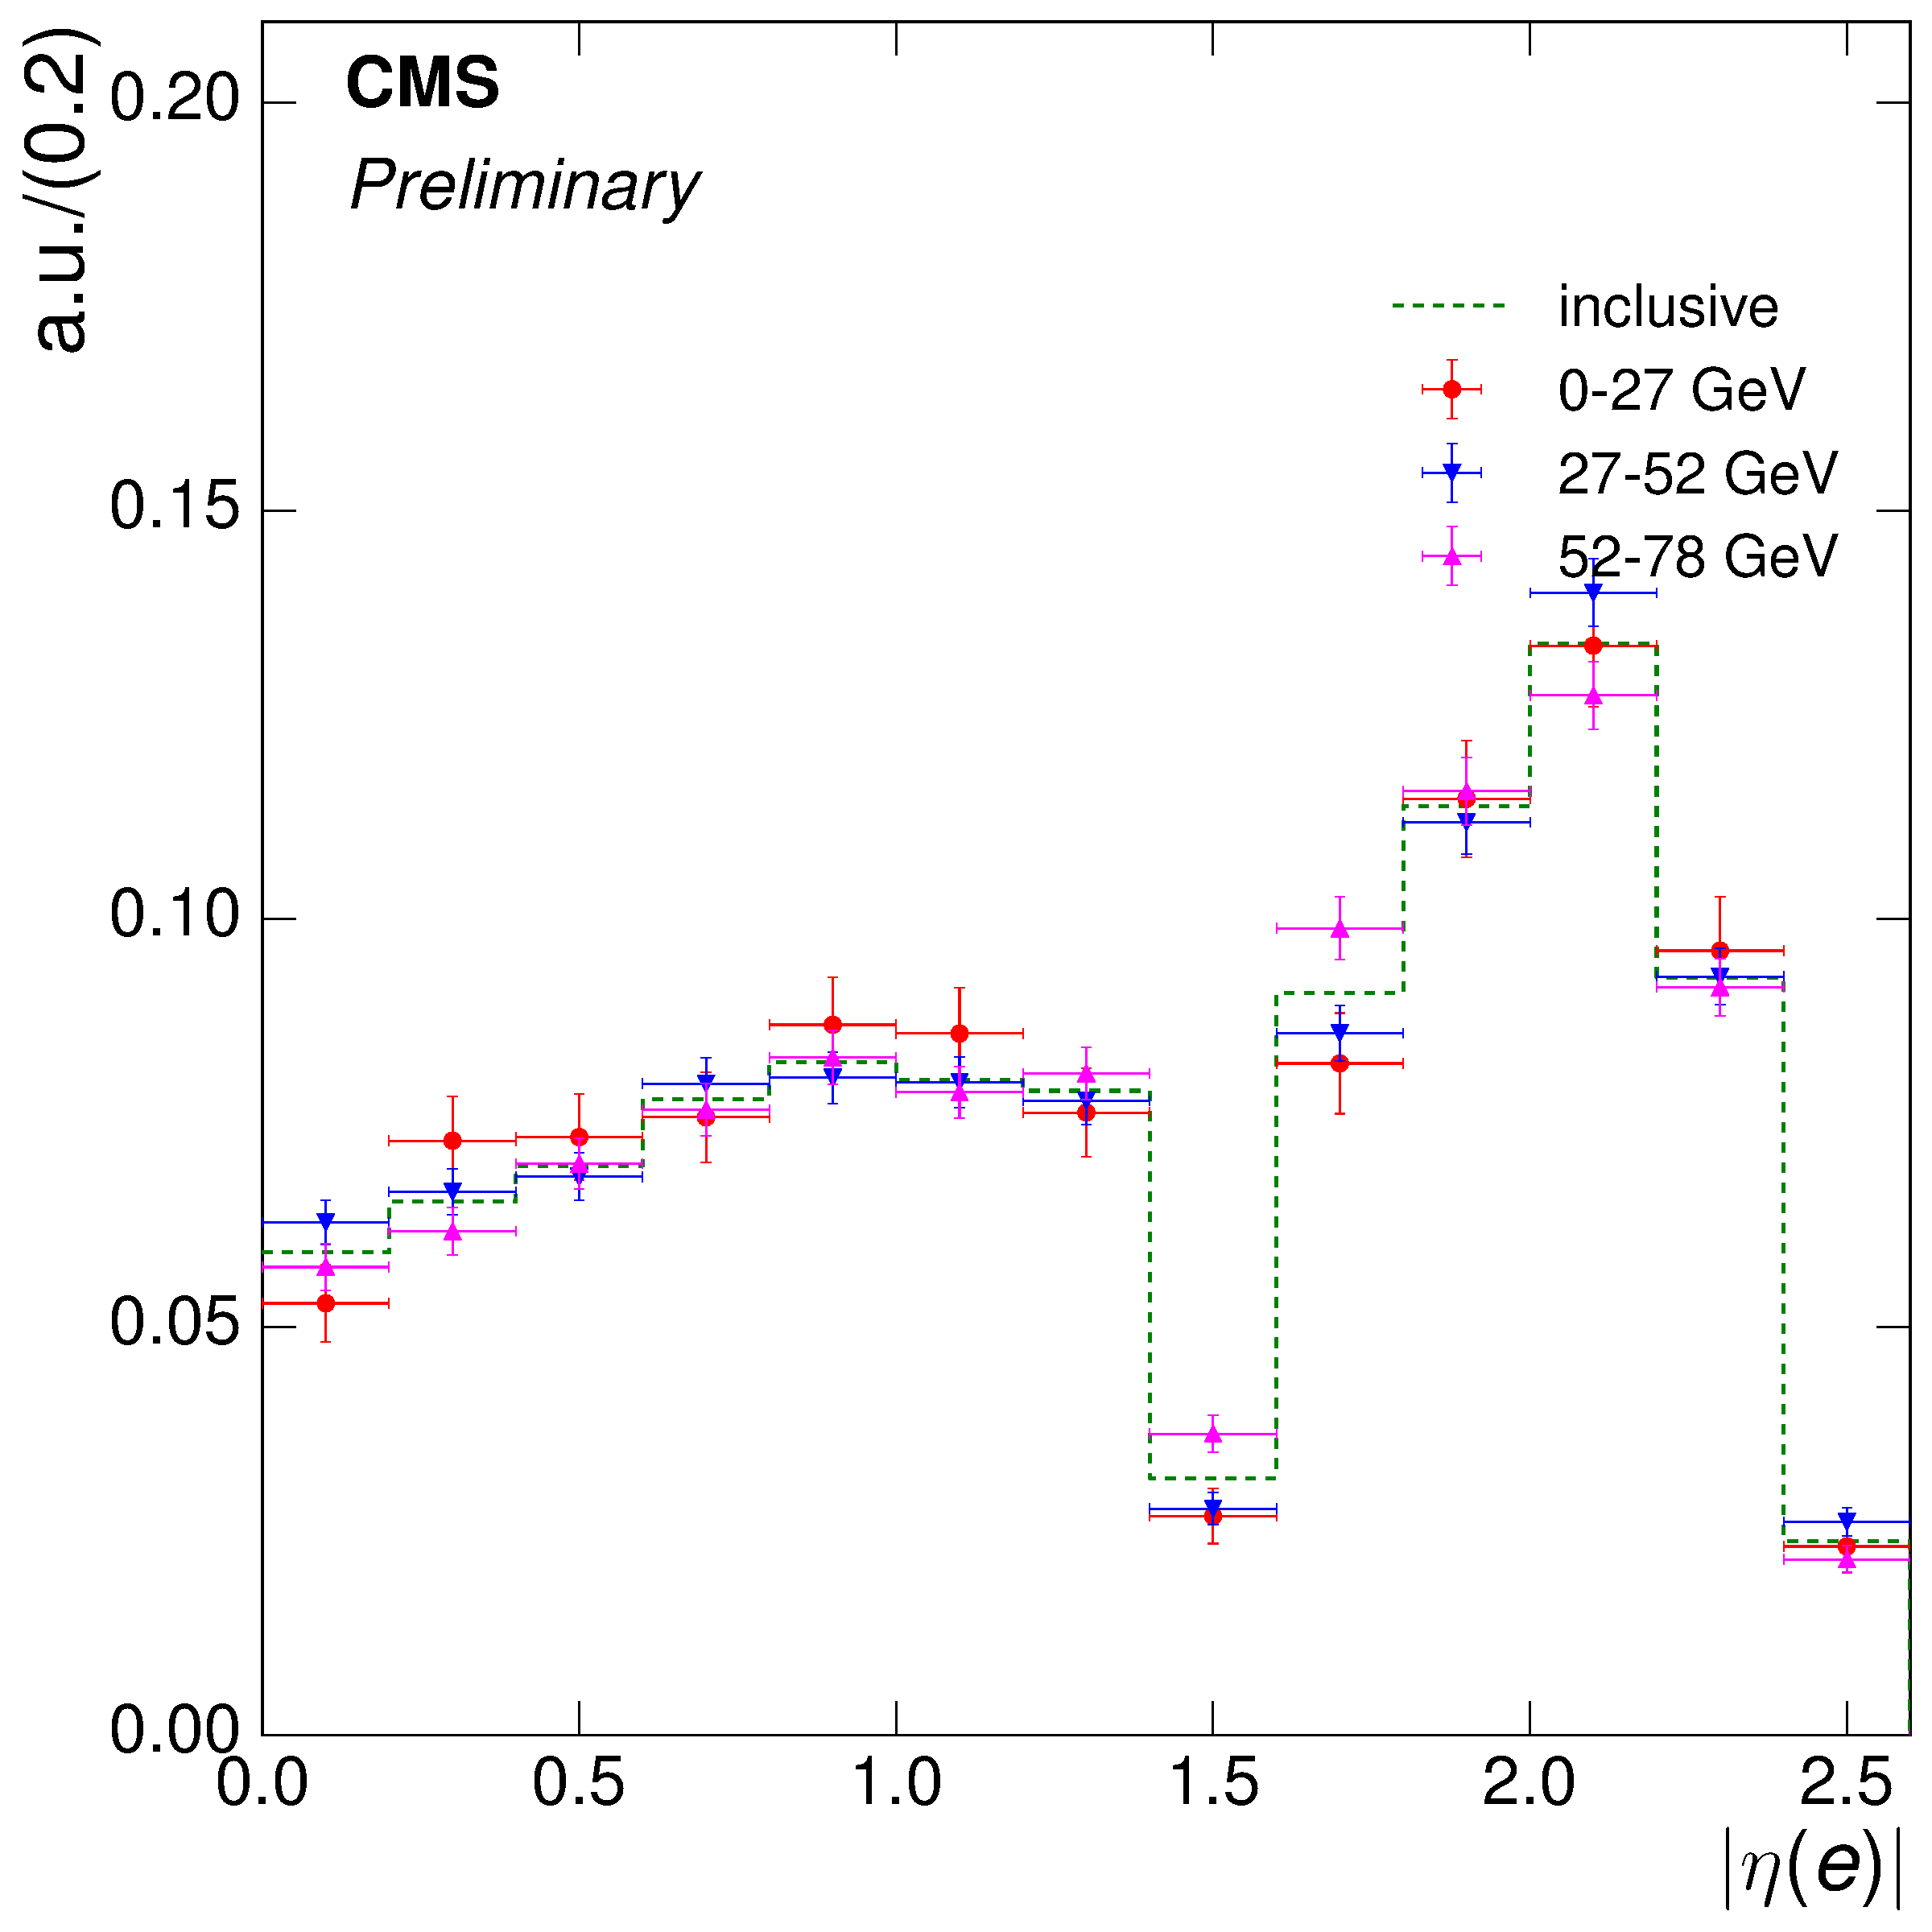
\includegraphics[width=0.48\textwidth]{Chapters/04_Analysis/04b_XSections/images/8TeV/fit_variables/electron/WPT/electron_absolute_eta/qcd/WPT_electron_absolute_eta_0orMoreBtag_QCD_template_comparison.pdf}\hfill
     \includegraphics[width=0.48\textwidth]{Chapters/04_Analysis/04b_XSections/images/8TeV/fit_variables/electron/WPT/angle_bl/qcd/WPT_angle_bl_1orMoreBtag_QCD_template_comparison.pdf}\\
     \includegraphics[width=0.48\textwidth]{Chapters/04_Analysis/04b_XSections/images/8TeV/fit_variables/electron/WPT/M3/qcd/WPT_M3_0orMoreBtag_QCD_template_comparison.pdf}\\
	 \caption{Normalised distributions of the QCD templates for the three fit variables at $\sqrt{s}=8\TeV$
	 inclusive across all \wpt bins and for the lowest three \wpt bins in the electron+jets channel: electron
	 \abseta (upper left), $\alpha$ (upper right) and M3 (lower right).}
     \label{fig:WPT_fit_variable_qcd_comparisons_electron_8TeV}
\end{figure}

\begin{figure}[hbtp]
    \centering
     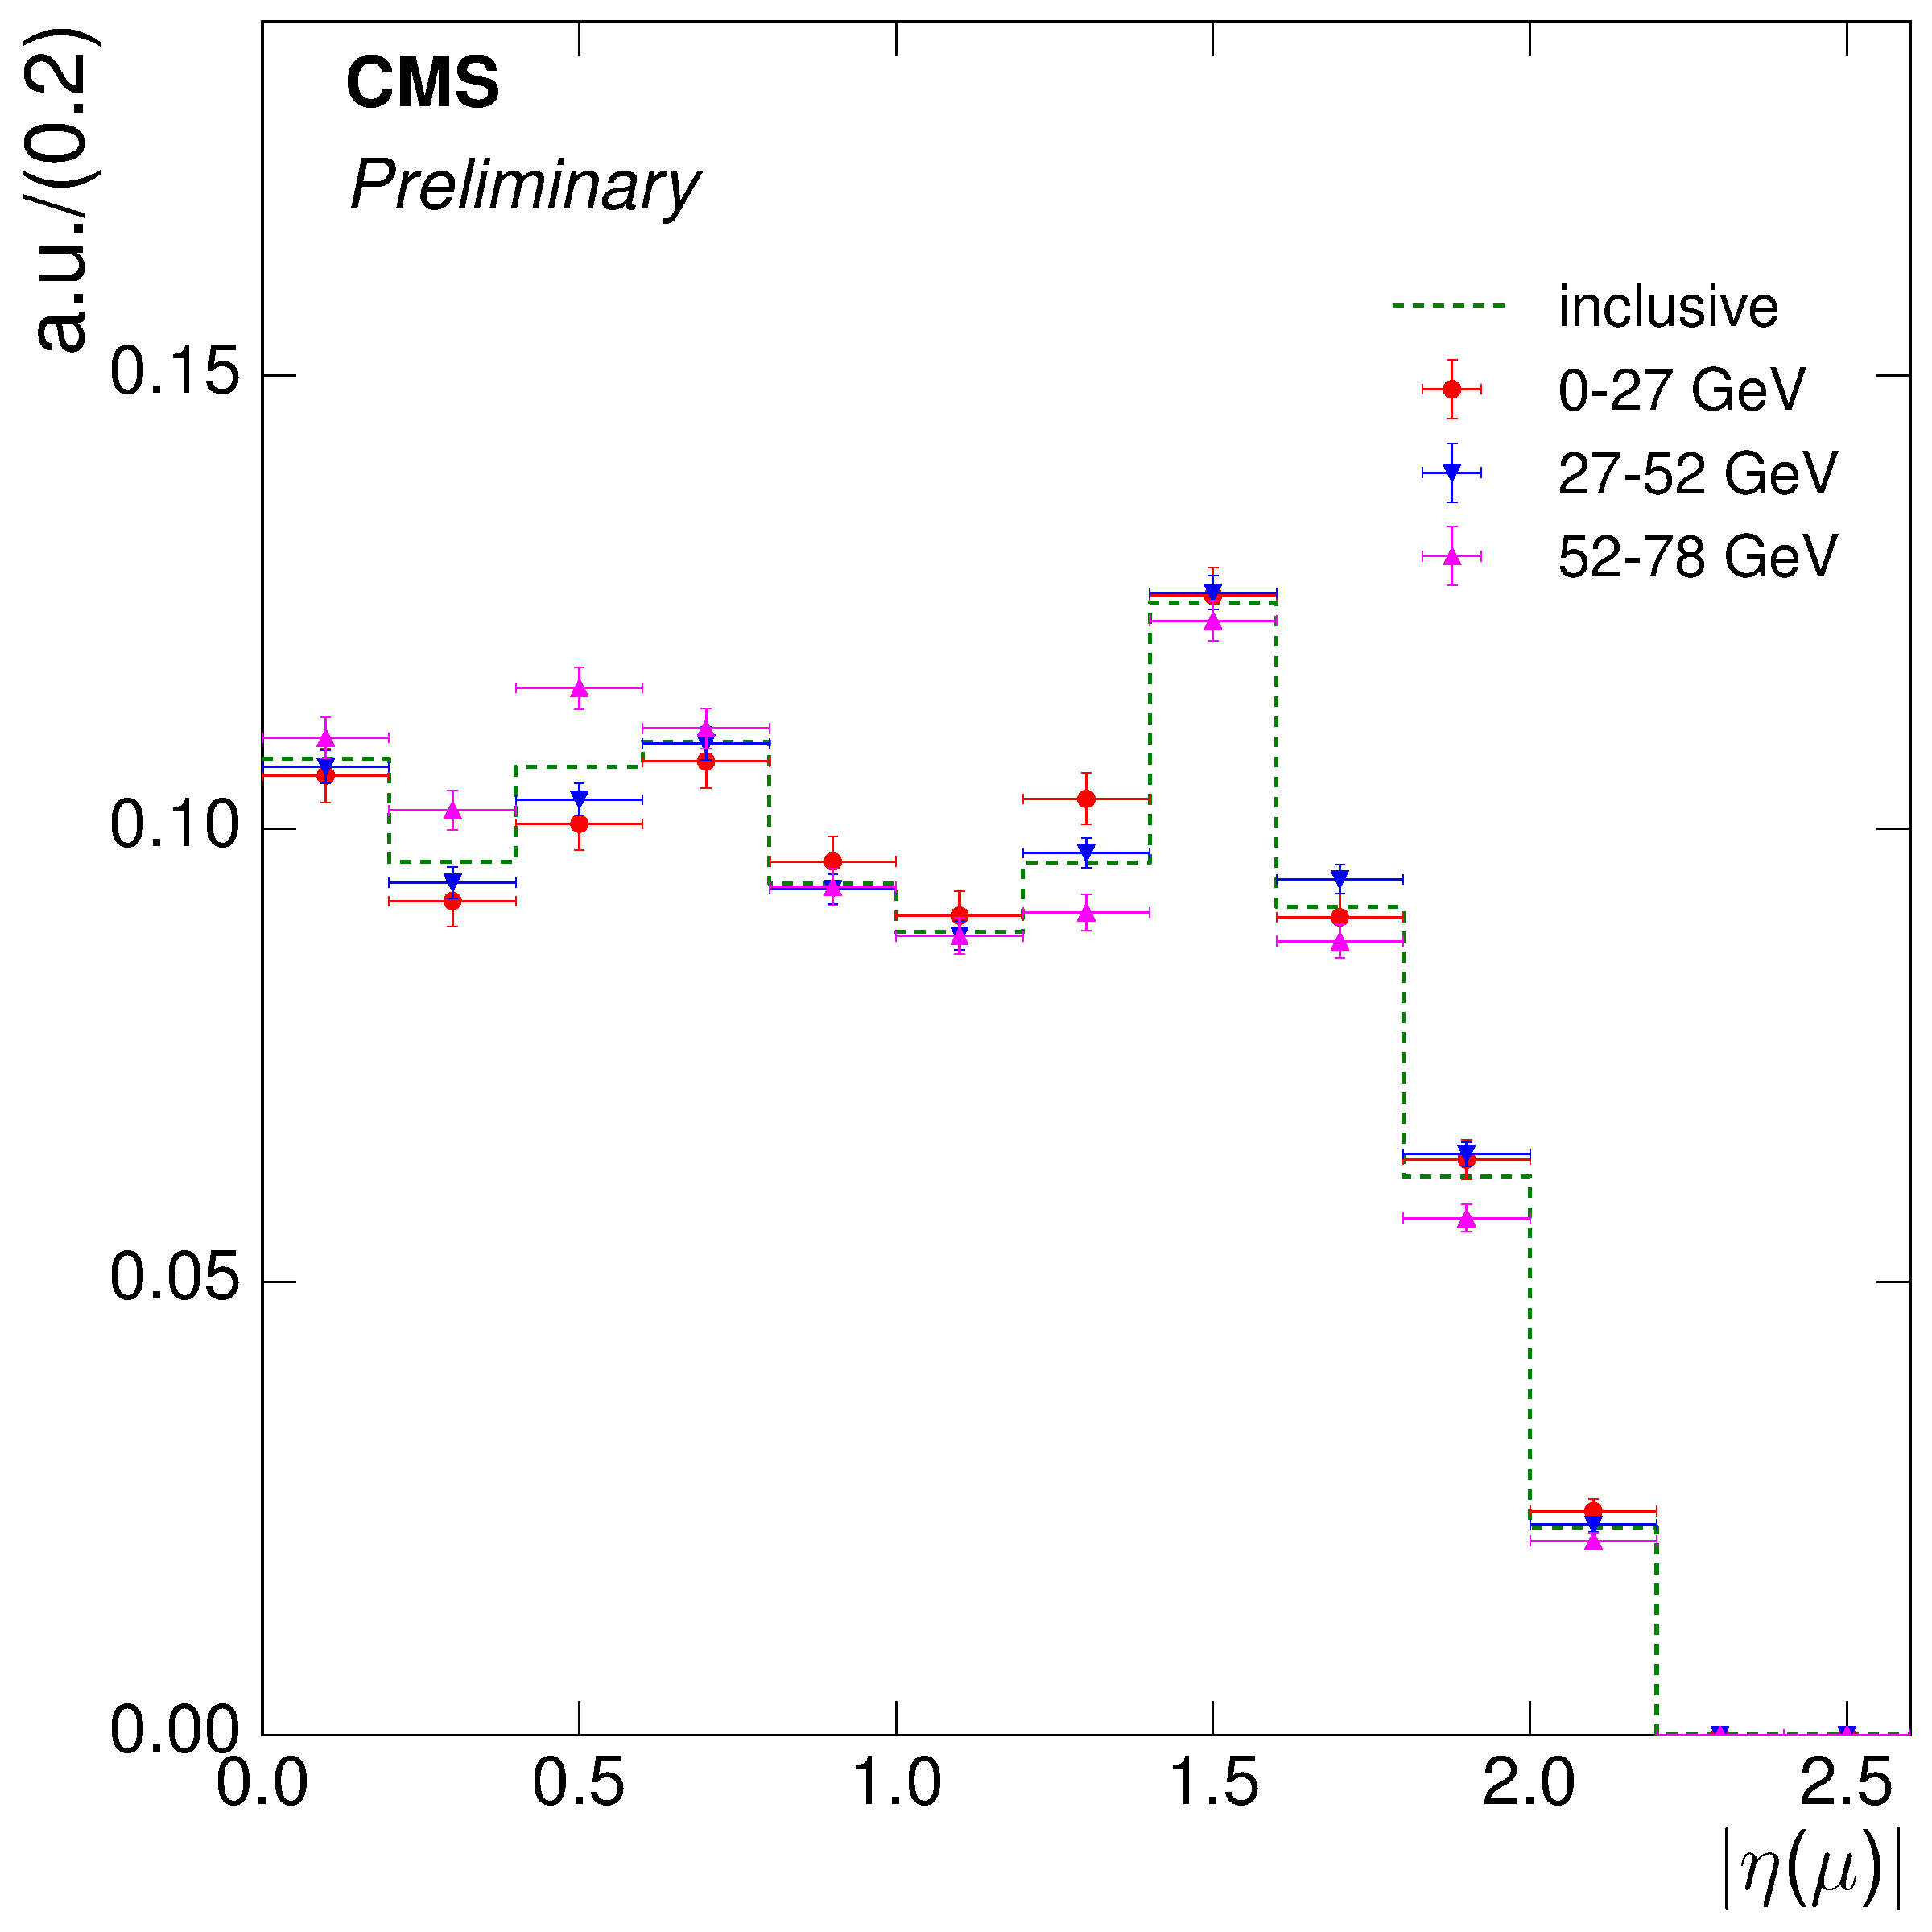
\includegraphics[width=0.48\textwidth]{Chapters/04_Analysis/04b_XSections/images/8TeV/fit_variables/muon/WPT/muon_absolute_eta/qcd/WPT_muon_absolute_eta_0orMoreBtag_QCD_template_comparison.pdf}\hfill
     \includegraphics[width=0.48\textwidth]{Chapters/04_Analysis/04b_XSections/images/8TeV/fit_variables/muon/WPT/angle_bl/qcd/WPT_angle_bl_1orMoreBtag_QCD_template_comparison.pdf}\\
     \includegraphics[width=0.48\textwidth]{Chapters/04_Analysis/04b_XSections/images/8TeV/fit_variables/muon/WPT/M3/qcd/WPT_M3_0orMoreBtag_QCD_template_comparison.pdf}\\
	 \caption{Normalised distributions of the QCD templates for the three fit variables at $\sqrt{s}=8\TeV$
	 inclusive across all \wpt bins and for the lowest three \wpt bins in the muon+jets channel: muon \abseta
	 (upper left), $\alpha$ (upper right) and M3 (lower right).}
     \label{fig:WPT_fit_variable_qcd_comparisons_muon_8TeV}
\end{figure}

\clearpage


\section{Fitting variable V+jets background template comparisons}
\label{as:fitting_variable_vjets_template_comparisons}

\begin{figure}[hbtp]
    \centering
     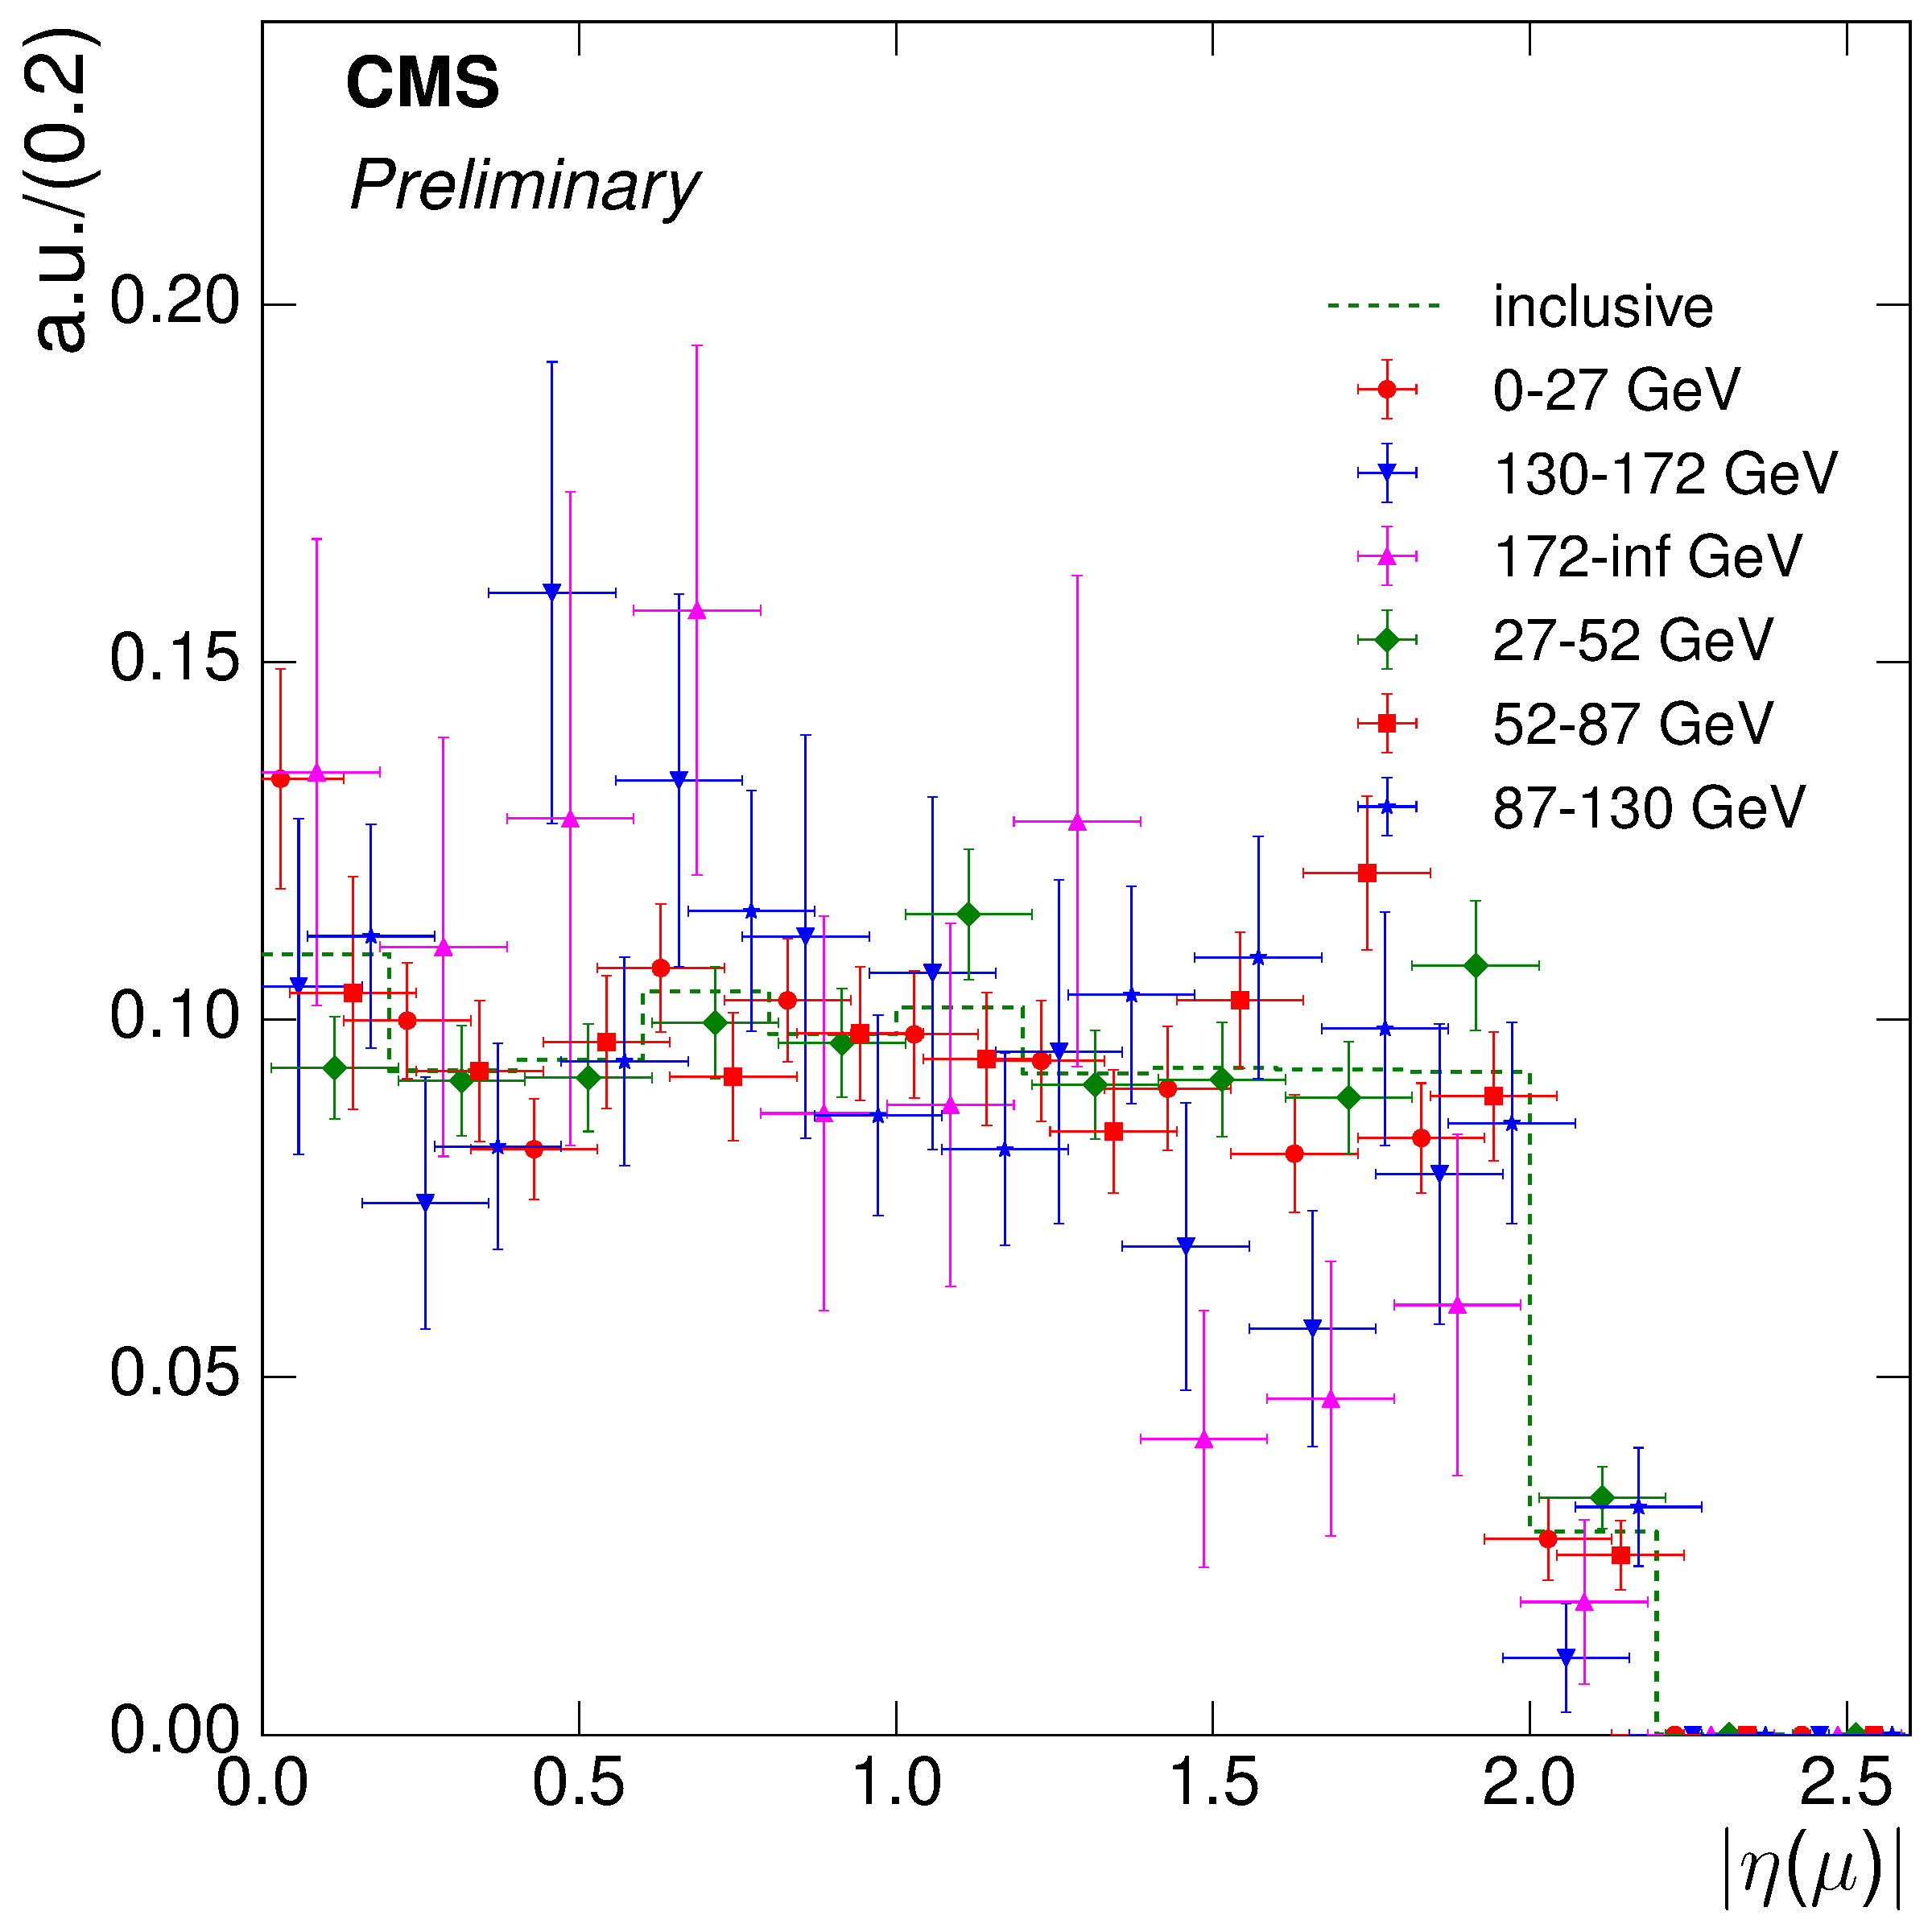
\includegraphics[width=0.48\textwidth]{Chapters/04_Analysis/04b_XSections/images/8TeV/fit_variables/muon/MET/muon_absolute_eta/vjets/MET_muon_absolute_eta_2orMoreBtags_VJets_template_comparison.pdf}\hfill
     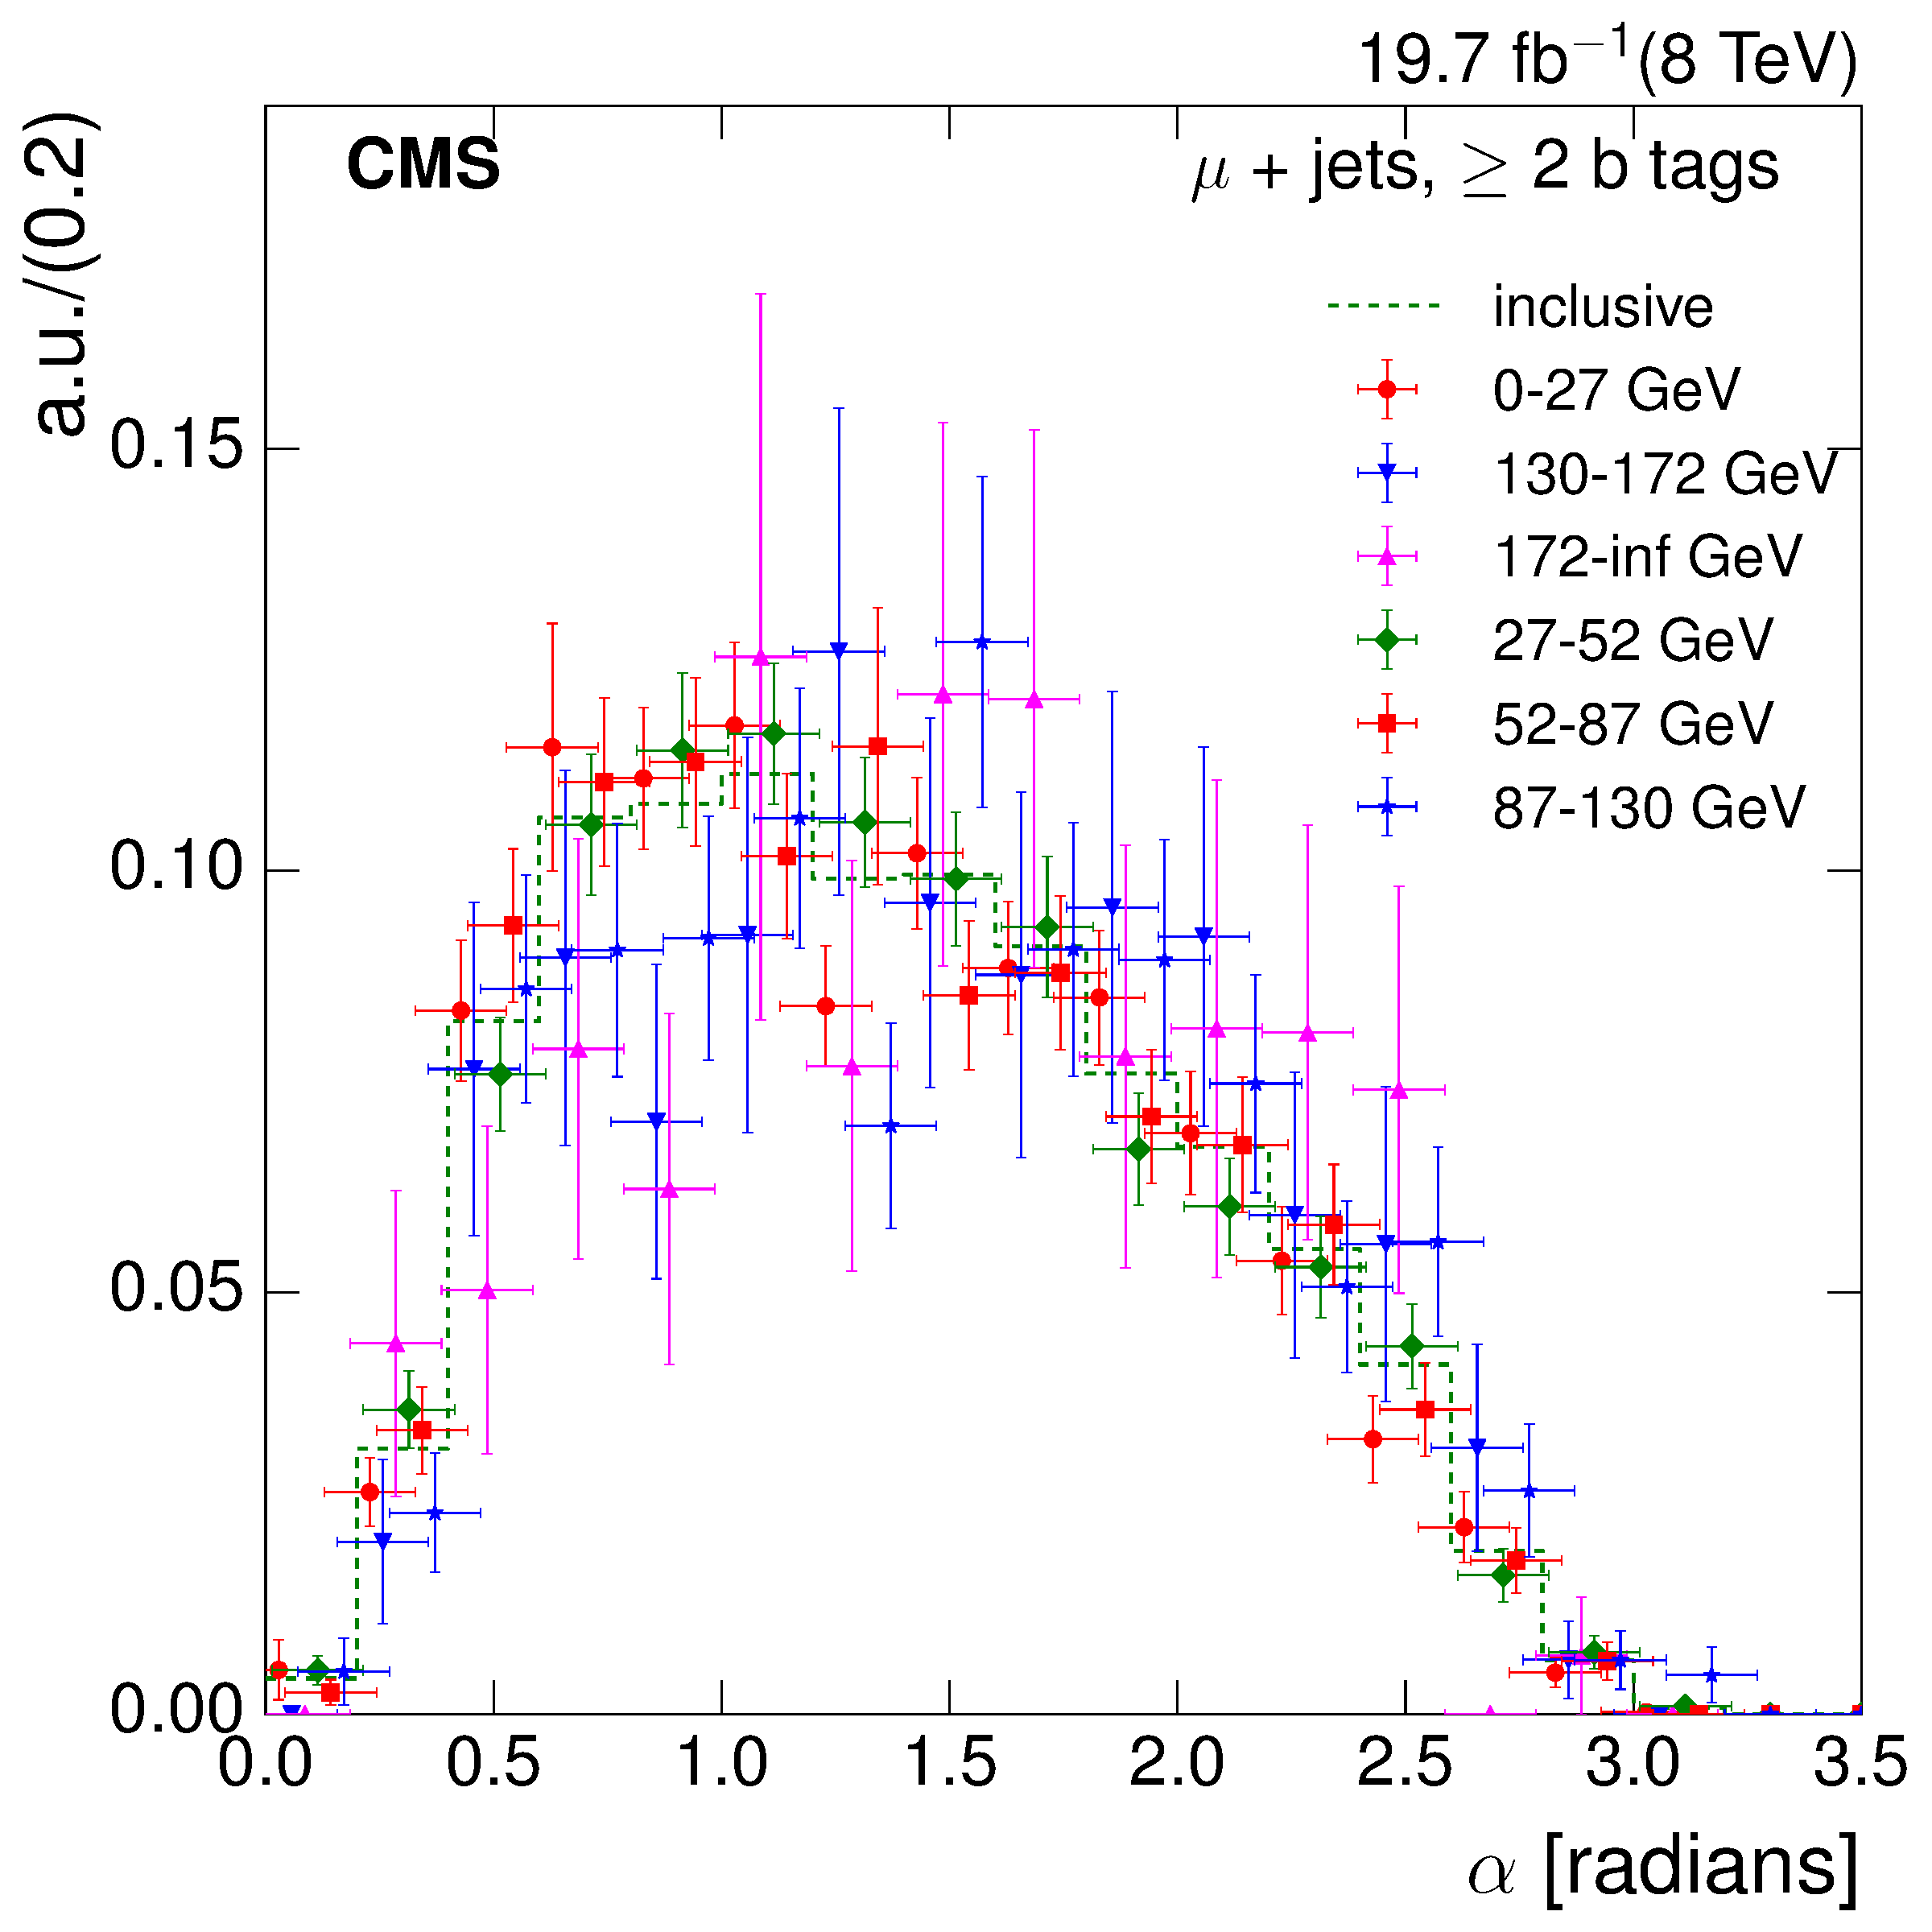
\includegraphics[width=0.48\textwidth]{Chapters/04_Analysis/04b_XSections/images/8TeV/fit_variables/muon/MET/angle_bl/vjets/MET_angle_bl_2orMoreBtags_VJets_template_comparison.pdf}\\
     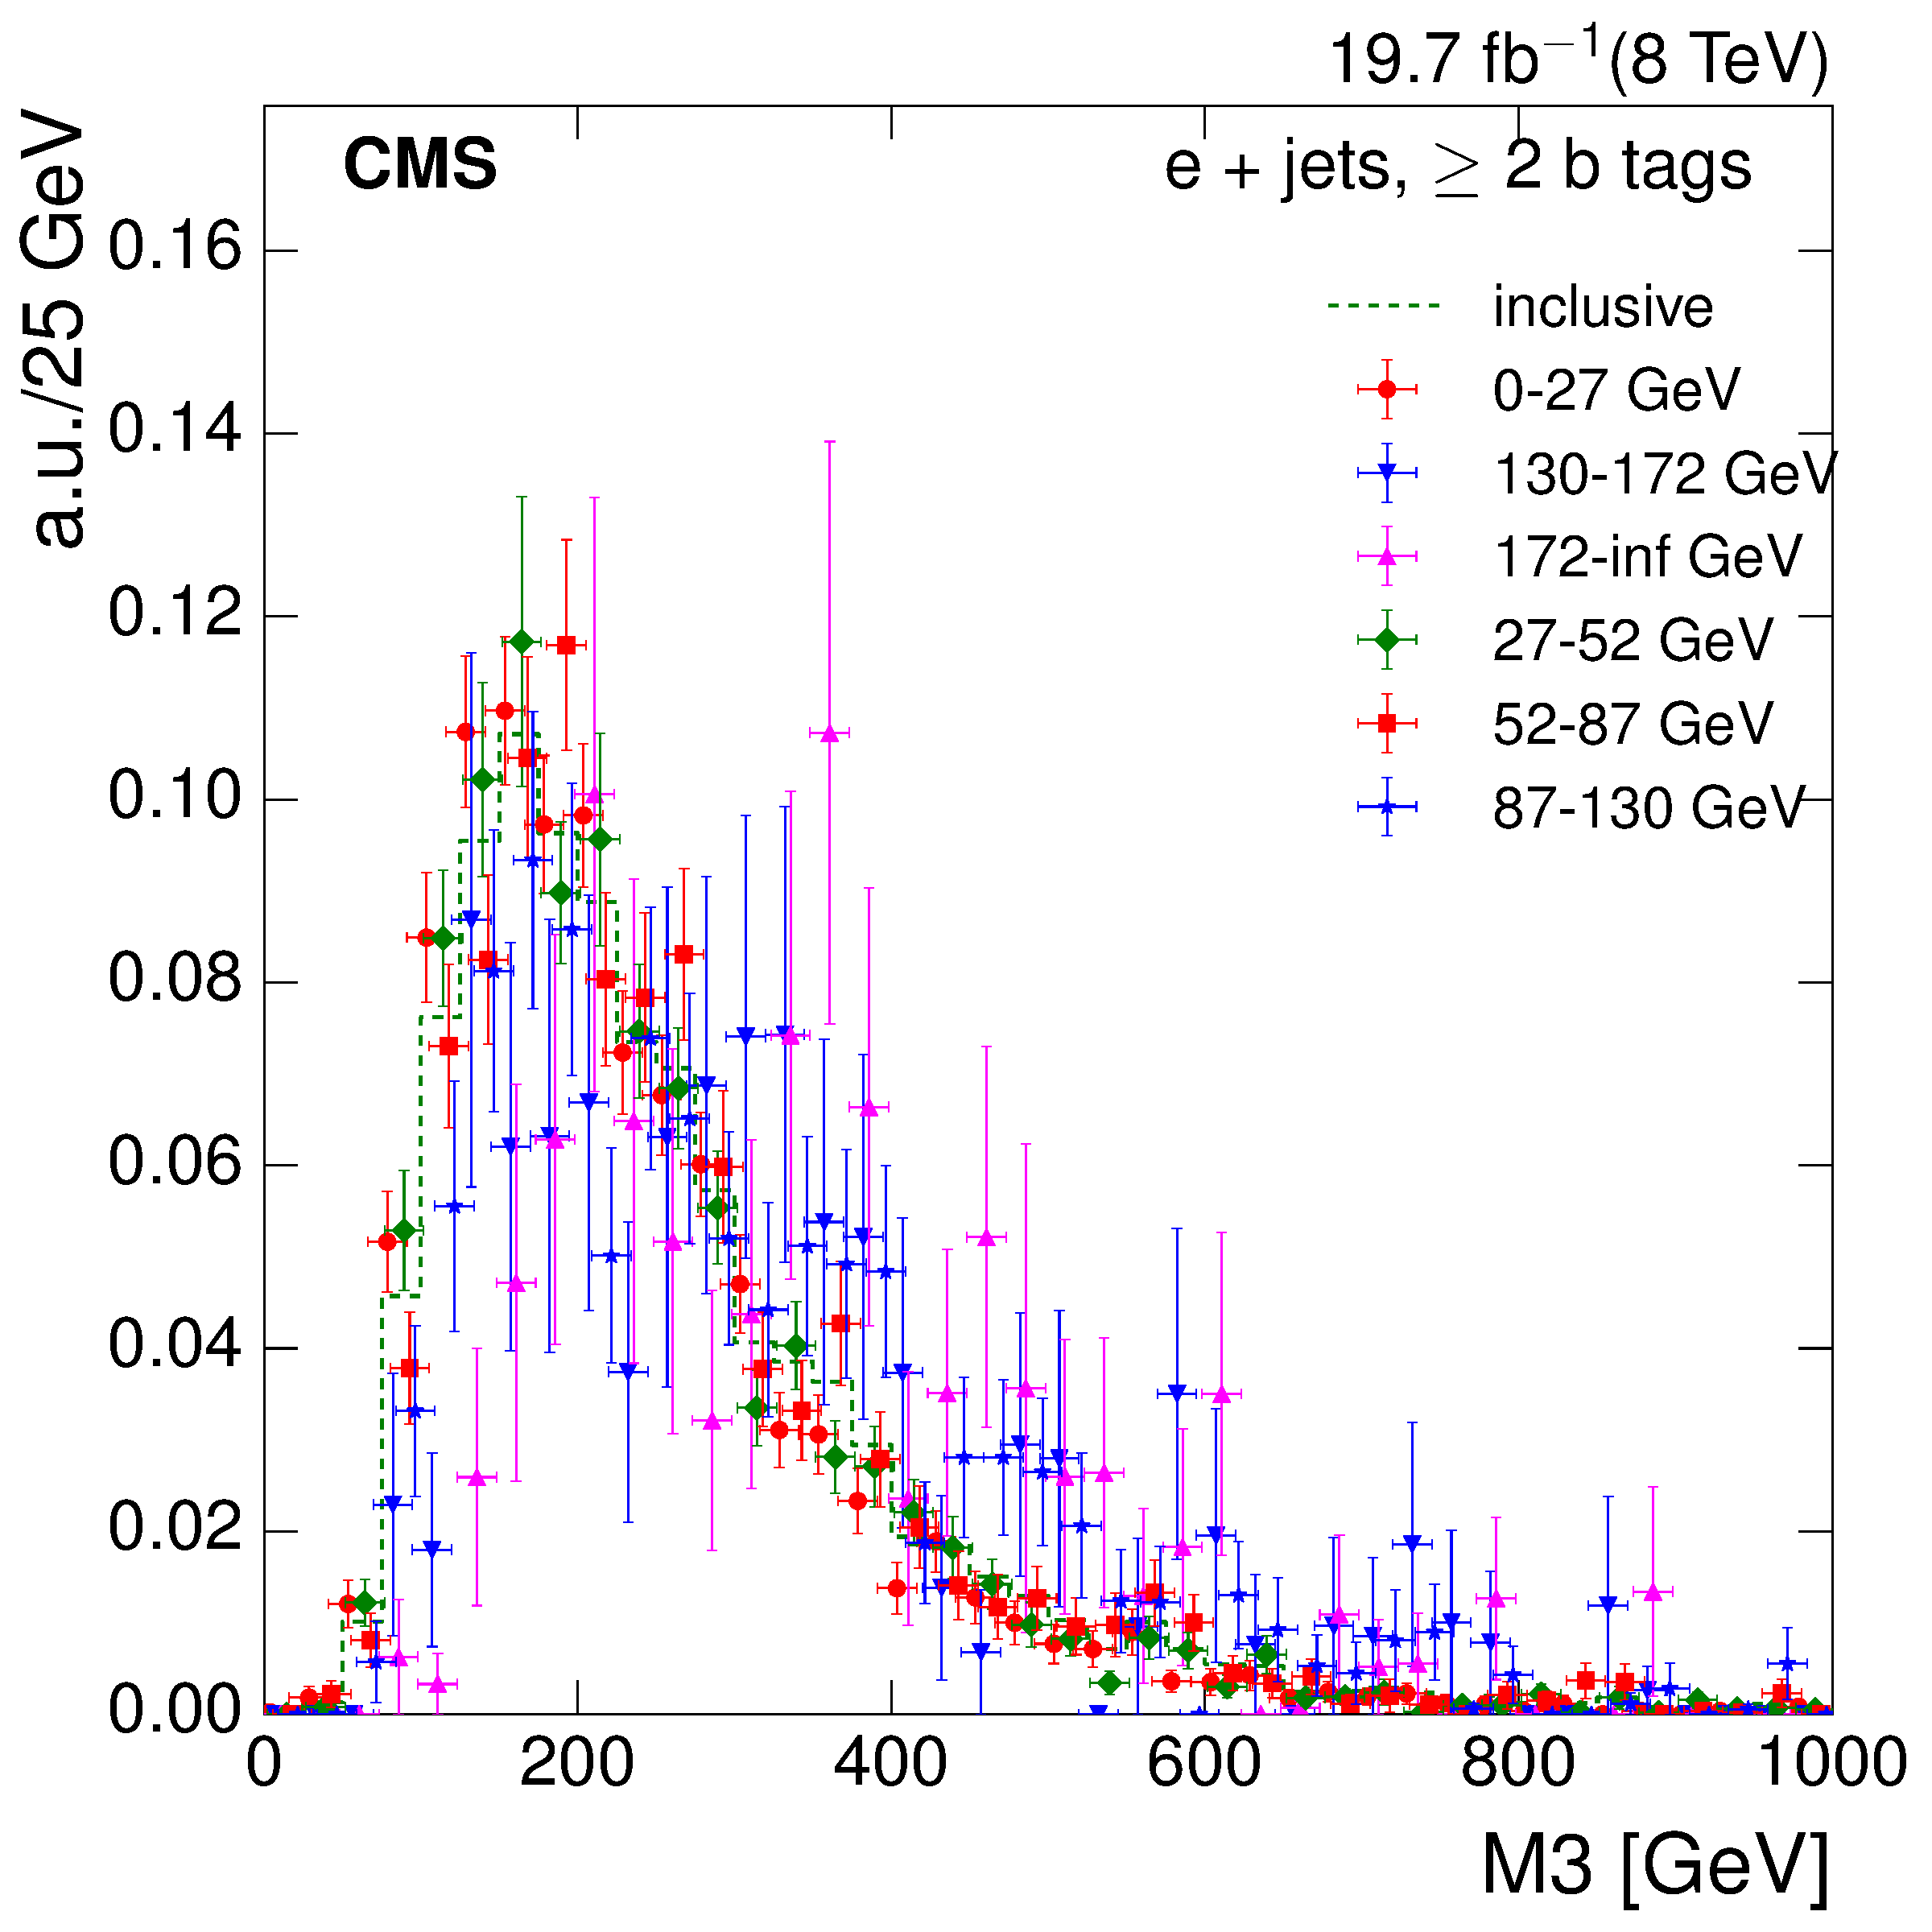
\includegraphics[width=0.48\textwidth]{Chapters/04_Analysis/04b_XSections/images/8TeV/fit_variables/muon/MET/M3/vjets/MET_M3_2orMoreBtags_VJets_template_comparison.pdf}\\
	 \caption{Normalised distributions of the V+jets templates for the three fit variables at $\sqrt{s}=8\TeV$
	 inclusive across all \met bins and for the lowest three \met bins in the muon+jets channel: muon
	 \abseta (upper left), $\alpha$ (upper right) and M3 (lower).}
     \label{fig:MET_fit_variable_vjets_comparisons_muon_8TeV}
\end{figure}

\begin{figure}[hbtp]
    \centering
     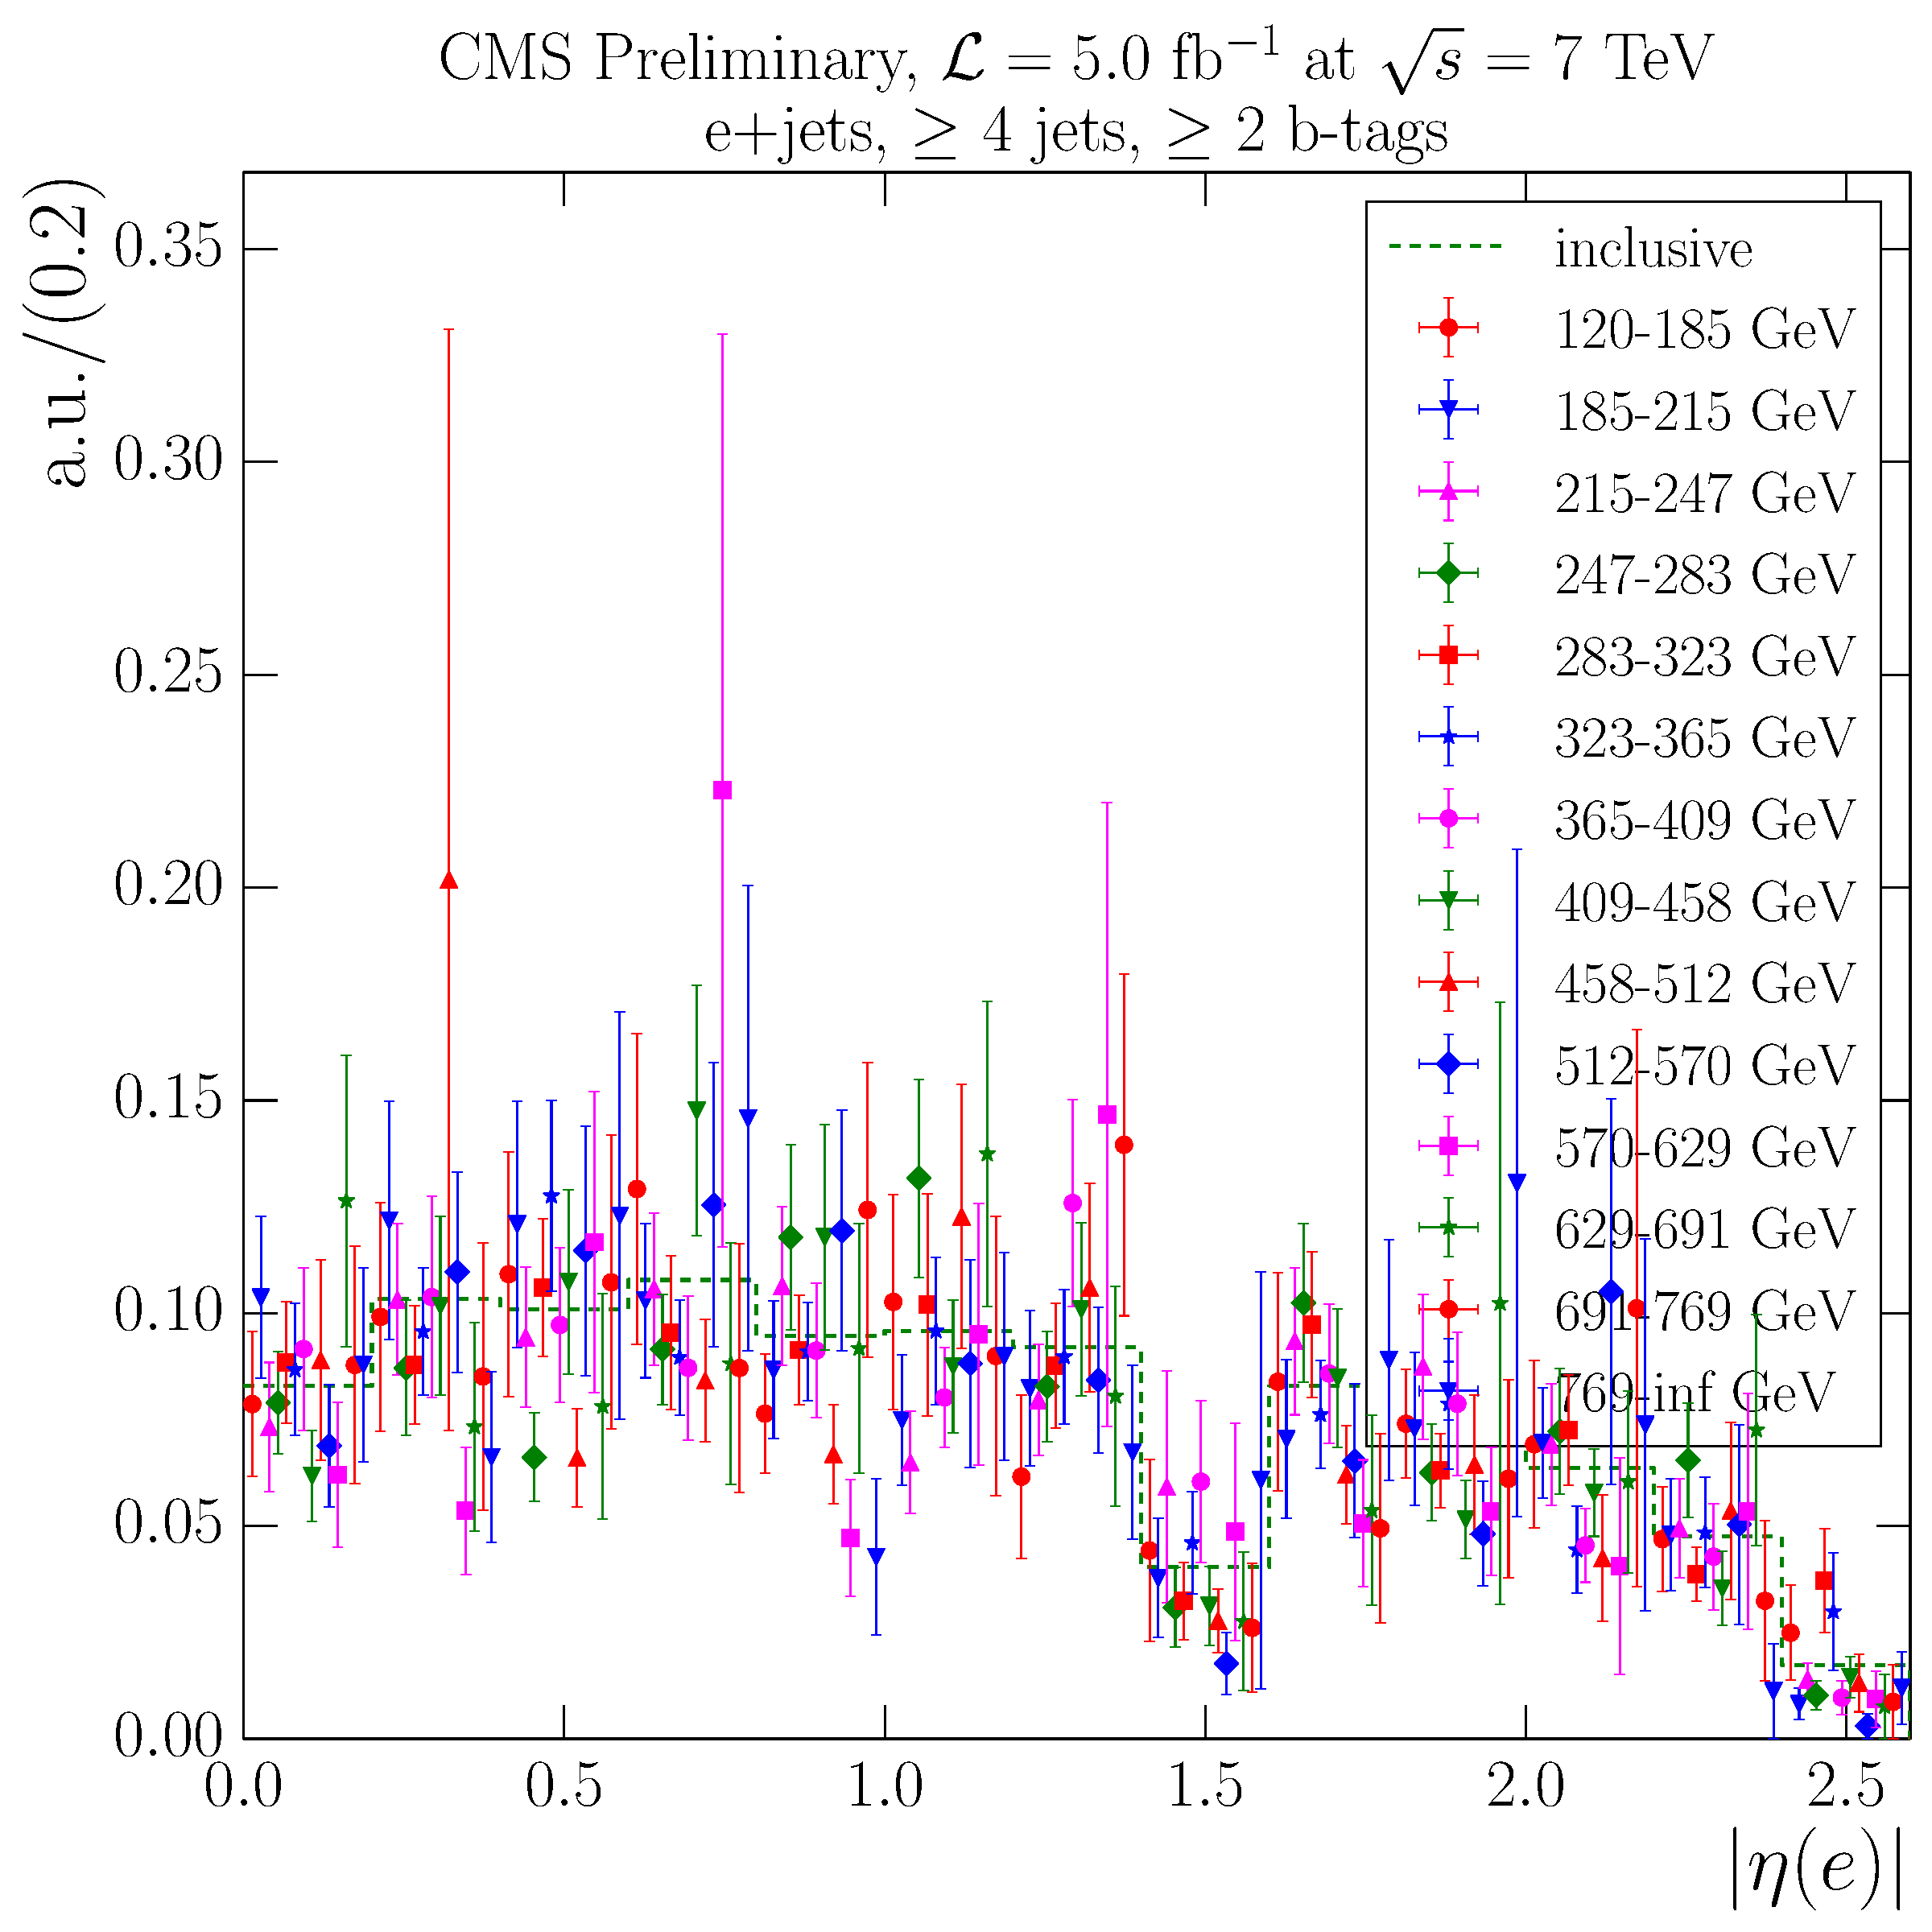
\includegraphics[width=0.48\textwidth]{Chapters/04_Analysis/04b_XSections/images/8TeV/fit_variables/electron/HT/electron_absolute_eta/vjets/HT_electron_absolute_eta_2orMoreBtags_VJets_template_comparison.pdf}\hfill
     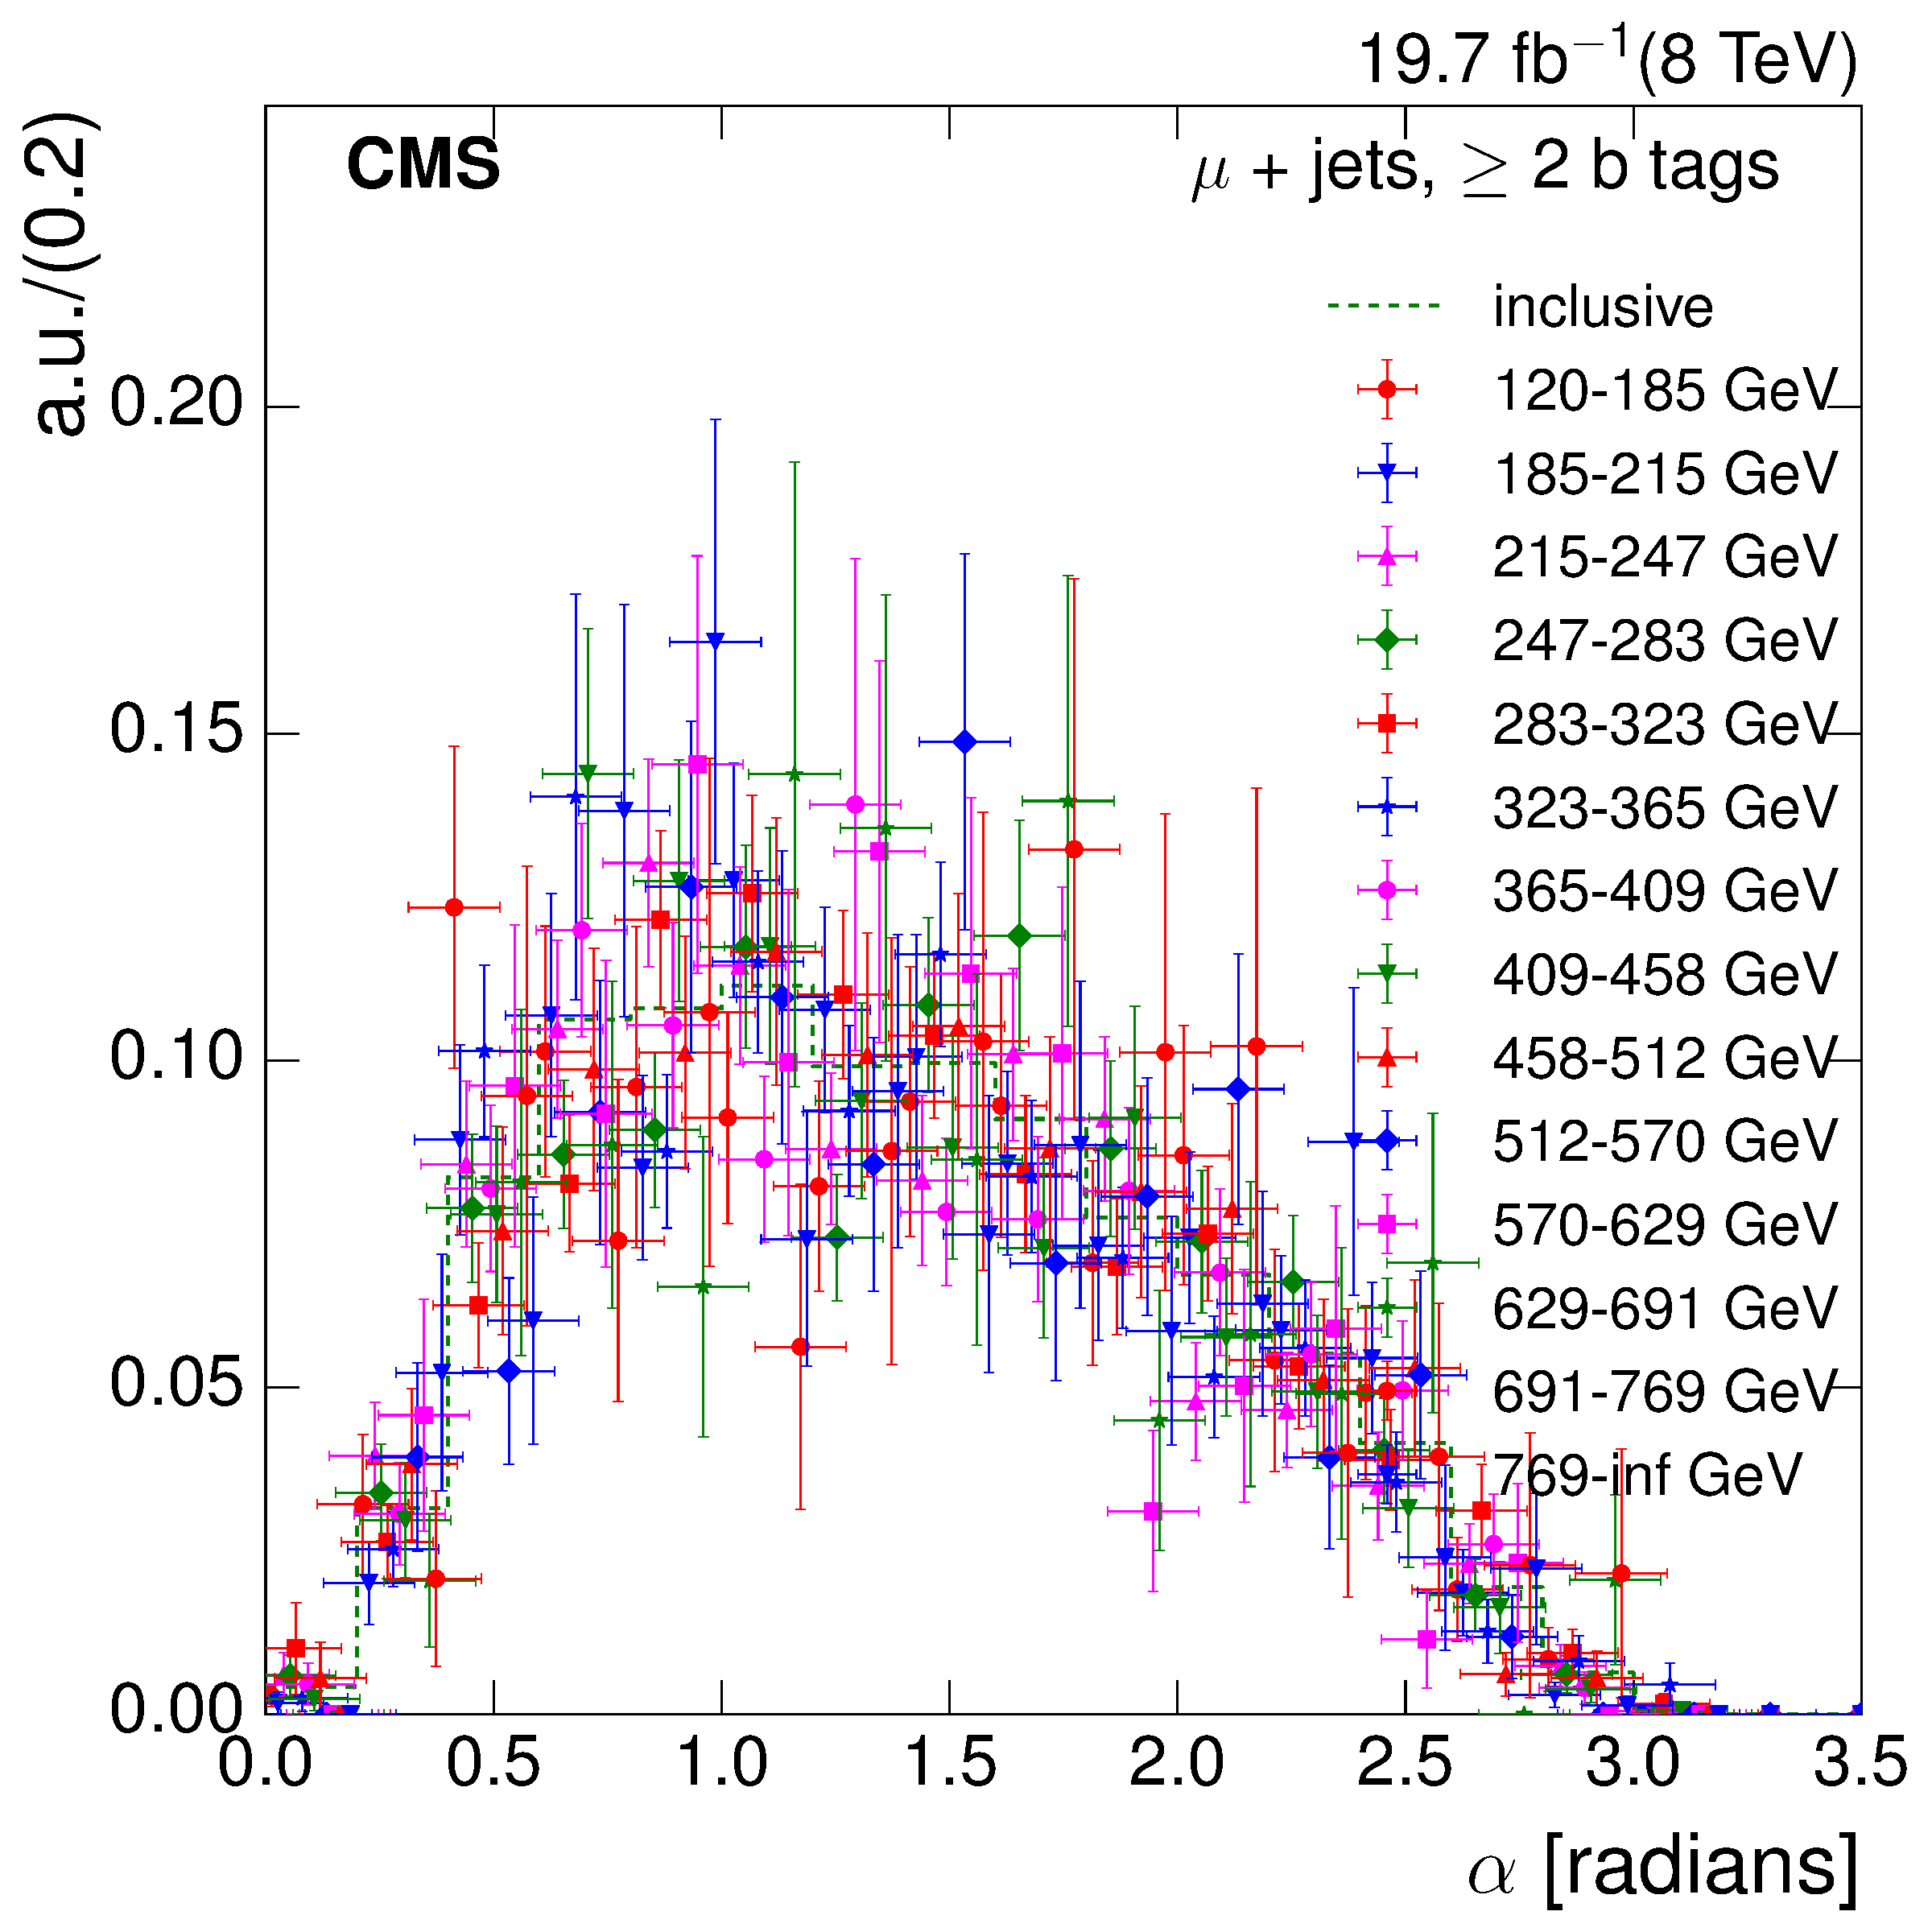
\includegraphics[width=0.48\textwidth]{Chapters/04_Analysis/04b_XSections/images/8TeV/fit_variables/electron/HT/angle_bl/vjets/HT_angle_bl_2orMoreBtags_VJets_template_comparison.pdf}\hfill
     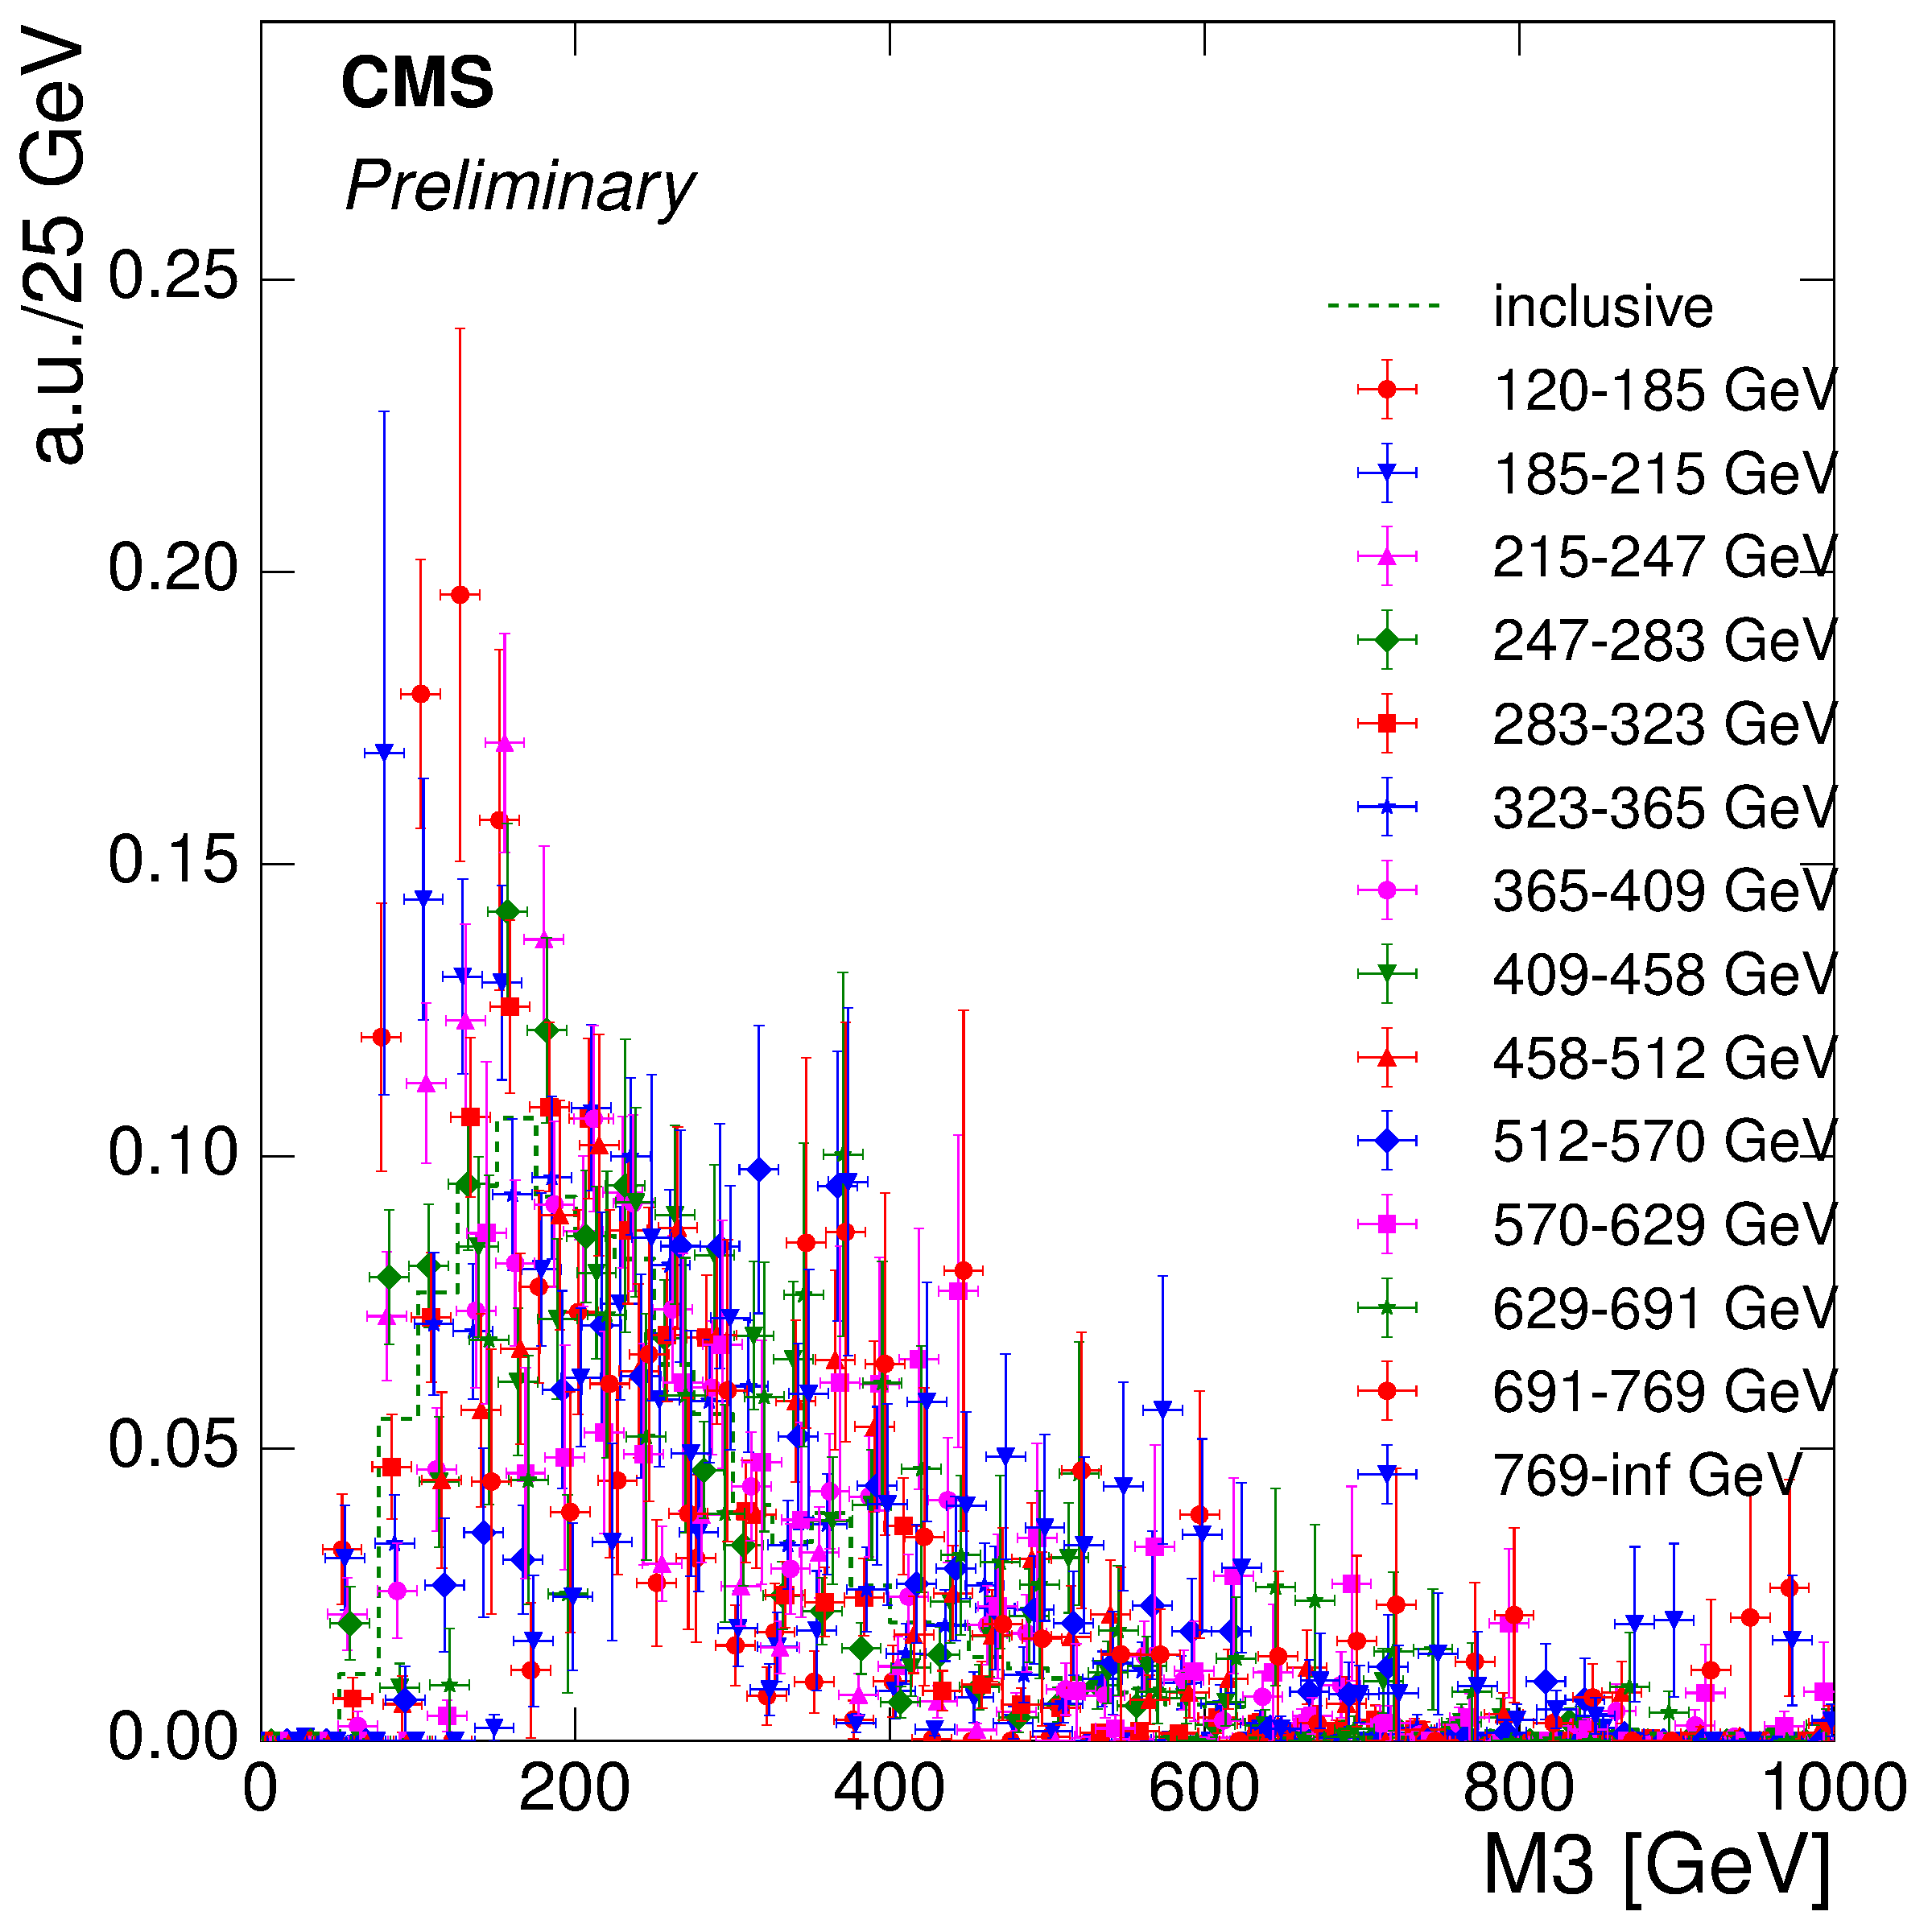
\includegraphics[width=0.48\textwidth]{Chapters/04_Analysis/04b_XSections/images/8TeV/fit_variables/electron/HT/M3/vjets/HT_M3_2orMoreBtags_VJets_template_comparison.pdf}\\
	 \caption{Normalised distributions of the V+jets templates for the three fit variables at $\sqrt{s}=8\TeV$
	 inclusive across all \HT bins and for individual \HT bins in the electron+jets channel: electron \abseta
	 (upper left), muon \abseta (upper right), $\alpha$ (lower left) and M3 (lower right).}
     \label{fig:HT_fit_variable_vjets_comparisons_electron_8TeV}
\end{figure}

\begin{figure}[hbtp]
    \centering
     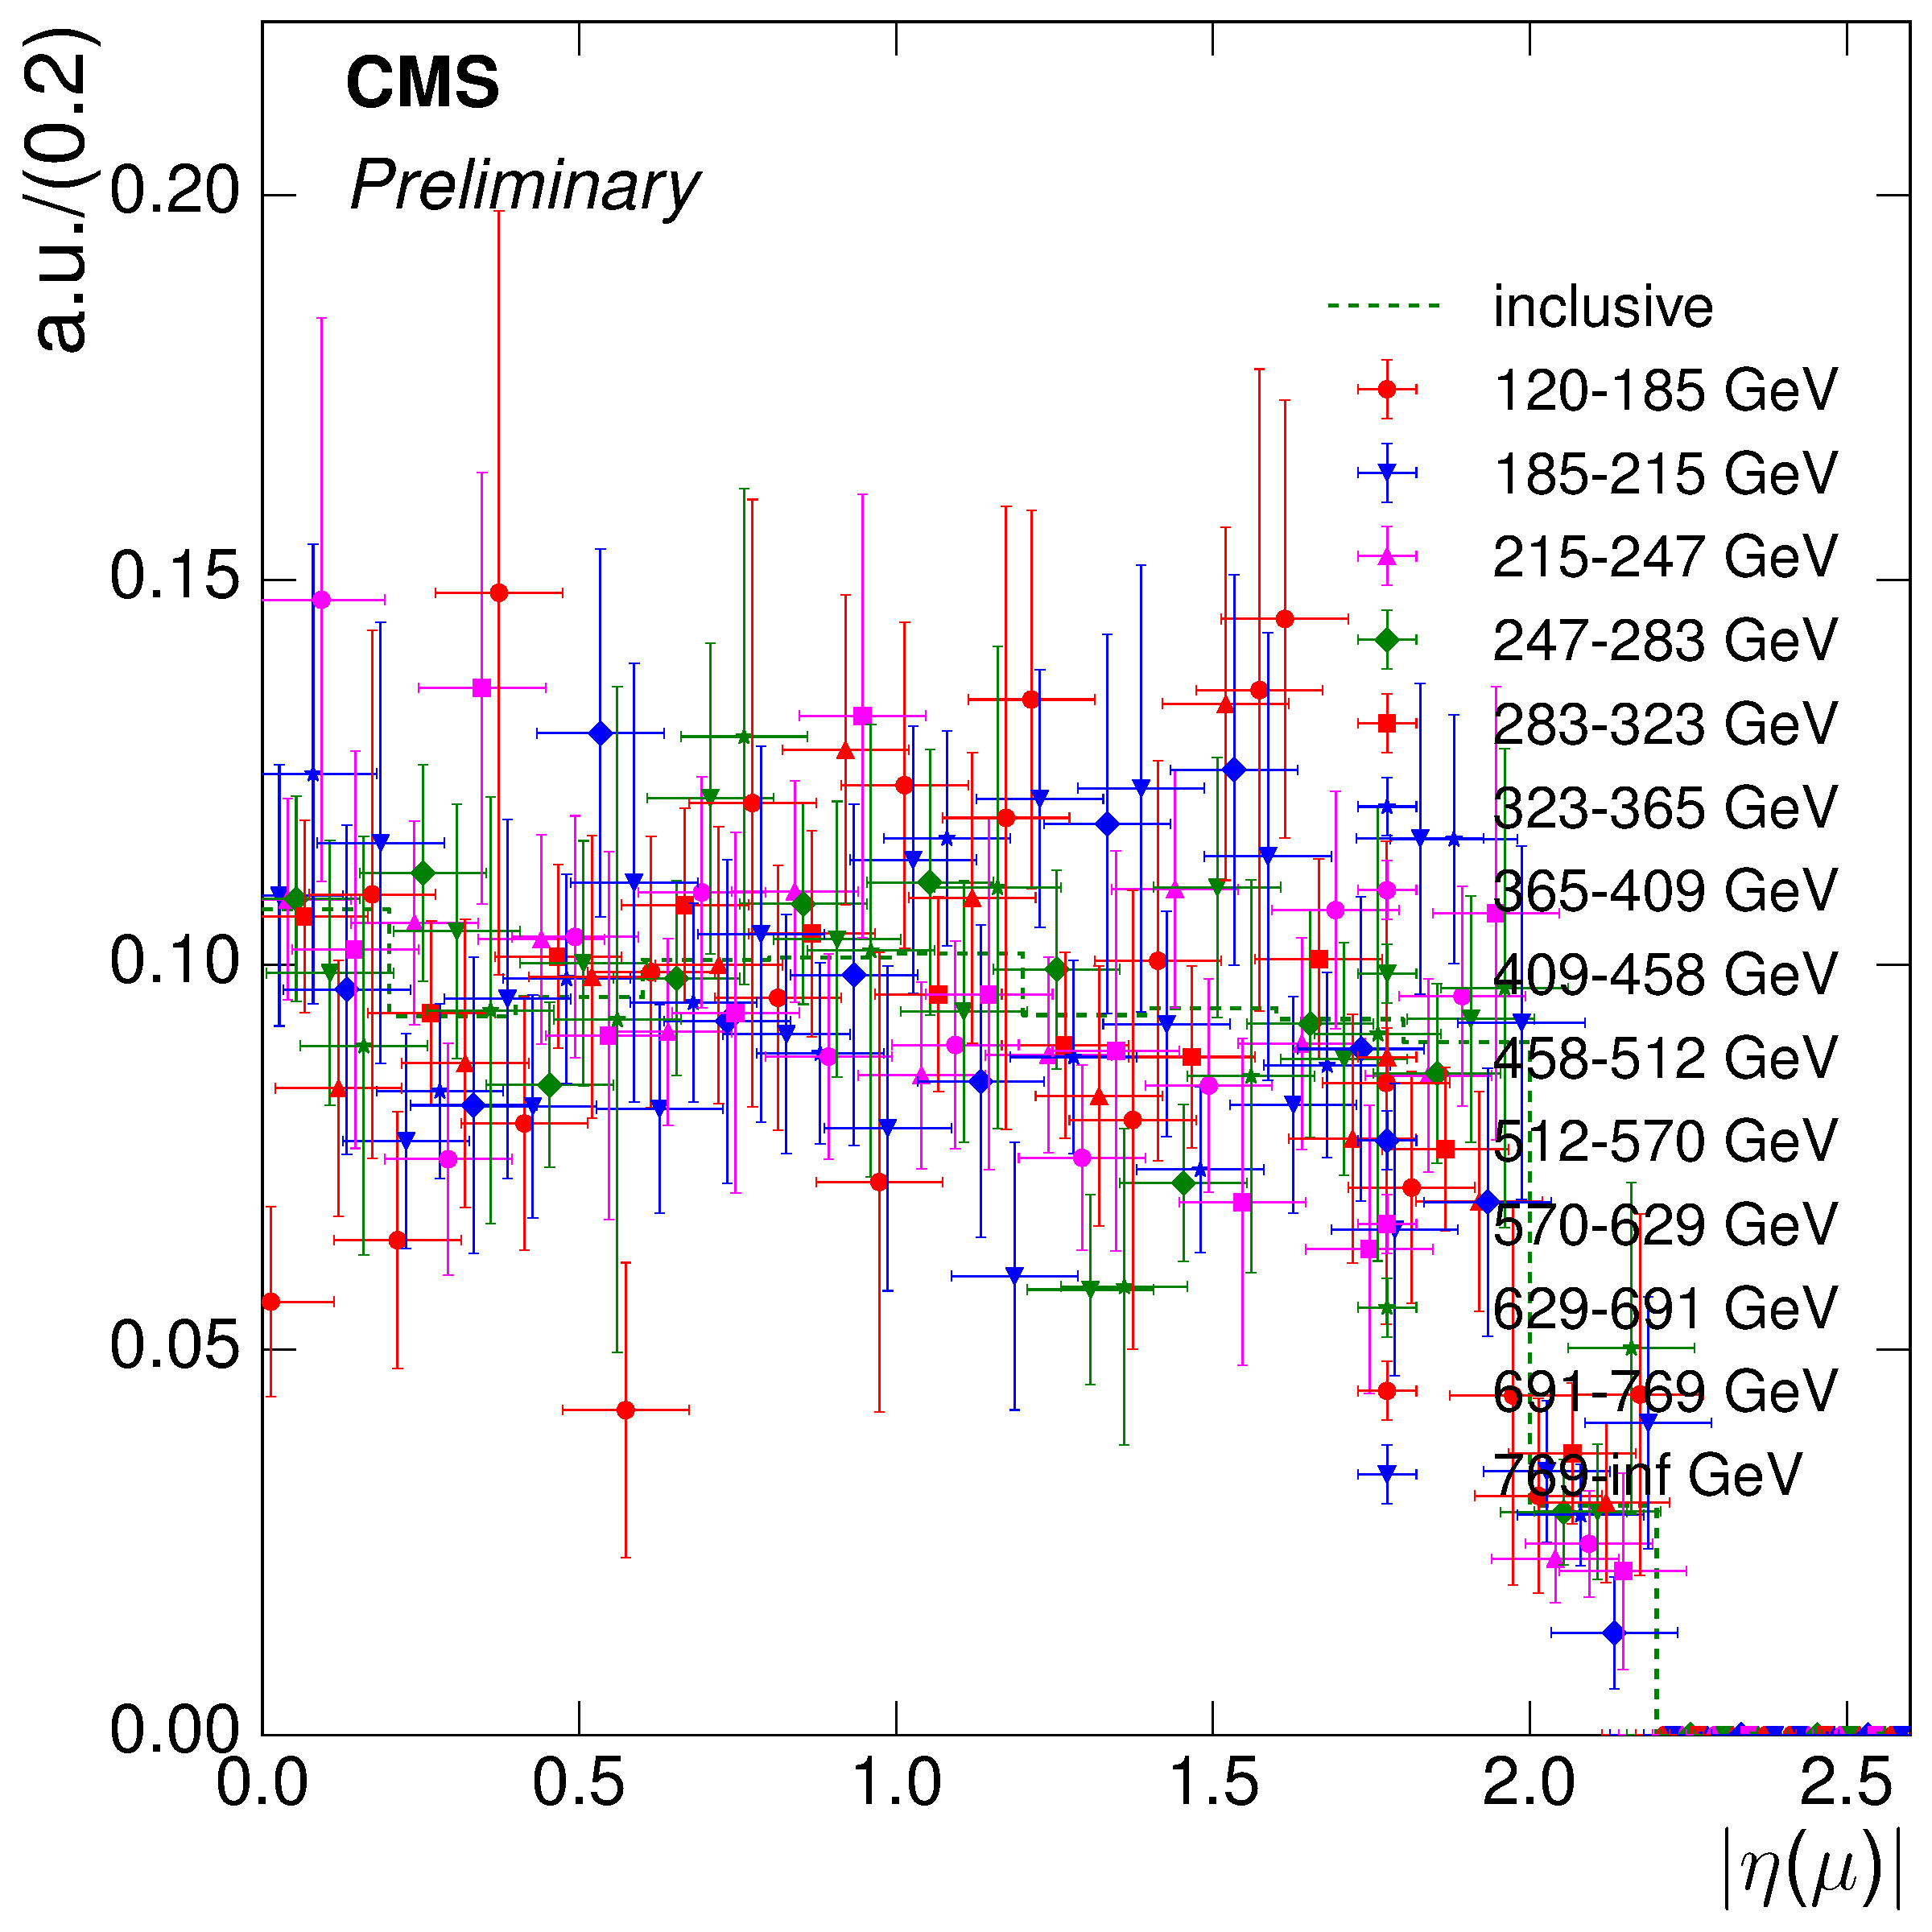
\includegraphics[width=0.48\textwidth]{Chapters/04_Analysis/04b_XSections/images/8TeV/fit_variables/muon/HT/muon_absolute_eta/vjets/HT_muon_absolute_eta_2orMoreBtags_VJets_template_comparison.pdf}\hfill
     \includegraphics[width=0.48\textwidth]{Chapters/04_Analysis/04b_XSections/images/8TeV/fit_variables/muon/HT/angle_bl/vjets/HT_angle_bl_2orMoreBtags_VJets_template_comparison.pdf}\hfill
     \includegraphics[width=0.48\textwidth]{Chapters/04_Analysis/04b_XSections/images/8TeV/fit_variables/muon/HT/M3/vjets/HT_M3_2orMoreBtags_VJets_template_comparison.pdf}\\
	 \caption{Normalised distributions of the V+jets templates for the three fit variables at $\sqrt{s}=8\TeV$
	 inclusive across all \HT bins and for individual \HT bins in the muon+jets channel: muon \abseta (upper
	 left), muon \abseta (upper right), $\alpha$ (lower left) and M3 (lower right).}
     \label{fig:HT_fit_variable_vjets_comparisons_muon_8TeV}
\end{figure}

\begin{figure}[hbtp]
    \centering
     \includegraphics[width=0.48\textwidth]{Chapters/04_Analysis/04b_XSections/images/8TeV/fit_variables/electron/ST/electron_absolute_eta/vjets/ST_electron_absolute_eta_2orMoreBtags_VJets_template_comparison.pdf}\hfill
     \includegraphics[width=0.48\textwidth]{Chapters/04_Analysis/04b_XSections/images/8TeV/fit_variables/electron/ST/angle_bl/vjets/ST_angle_bl_2orMoreBtags_VJets_template_comparison.pdf}\hfill
     \includegraphics[width=0.48\textwidth]{Chapters/04_Analysis/04b_XSections/images/8TeV/fit_variables/electron/ST/M3/vjets/ST_M3_2orMoreBtags_VJets_template_comparison.pdf}\\
	 \caption{Normalised distributions of the V+jets templates for the three fit variables at $\sqrt{s}=8\TeV$
	 inclusive across all \st bins and for individual \st bins in the electron+jets channel: electron \abseta
	 (upper left), muon \abseta (upper right), $\alpha$ (lower left) and M3 (lower right).}
     \label{fig:ST_fit_variable_vjets_comparisons_8TeV}
\end{figure}

\begin{figure}[hbtp]
    \centering
     \includegraphics[width=0.48\textwidth]{Chapters/04_Analysis/04b_XSections/images/8TeV/fit_variables/muon/ST/muon_absolute_eta/vjets/ST_muon_absolute_eta_2orMoreBtags_VJets_template_comparison.pdf}\hfill
     \includegraphics[width=0.48\textwidth]{Chapters/04_Analysis/04b_XSections/images/8TeV/fit_variables/muon/ST/angle_bl/vjets/ST_angle_bl_2orMoreBtags_VJets_template_comparison.pdf}\hfill
     \includegraphics[width=0.48\textwidth]{Chapters/04_Analysis/04b_XSections/images/8TeV/fit_variables/muon/ST/M3/vjets/ST_M3_2orMoreBtags_VJets_template_comparison.pdf}\\
	 \caption{Normalised distributions of the V+jets templates for the three fit variables at $\sqrt{s}=8\TeV$
	 inclusive across all \st bins and for individual \st bins in the muon+jets channel: muon \abseta (upper
	 left), $\alpha$ (upper right) and M3 (lower right).}
     \label{fig:ST_fit_variable_vjets_comparisons_muon_8TeV}
\end{figure}


\begin{figure}[hbtp]
    \centering
     \includegraphics[width=0.48\textwidth]{Chapters/04_Analysis/04b_XSections/images/8TeV/fit_variables/electron/MT/electron_absolute_eta/vjets/MT_electron_absolute_eta_2orMoreBtags_VJets_template_comparison.pdf}\hfill
     \includegraphics[width=0.48\textwidth]{Chapters/04_Analysis/04b_XSections/images/8TeV/fit_variables/electron/MT/angle_bl/vjets/MT_angle_bl_2orMoreBtags_VJets_template_comparison.pdf}\hfill
     \includegraphics[width=0.48\textwidth]{Chapters/04_Analysis/04b_XSections/images/8TeV/fit_variables/electron/MT/M3/vjets/MT_M3_2orMoreBtags_VJets_template_comparison.pdf}\\
	 \caption{Normalised distributions of the V+jets templates for the three fit variables at $\sqrt{s}=8\TeV$
	 inclusive across all \mt bins and for individual \mt bins in the electron+jets channel: electron \abseta
	 (upper left), $\alpha$ (upper right) and M3 (lower).}
     \label{fig:MT_fit_variable_vjets_comparisons_electron_8TeV}
\end{figure}

\begin{figure}[hbtp]
    \centering
     \includegraphics[width=0.48\textwidth]{Chapters/04_Analysis/04b_XSections/images/8TeV/fit_variables/muon/MT/muon_absolute_eta/vjets/MT_muon_absolute_eta_2orMoreBtags_VJets_template_comparison.pdf}\hfill
     \includegraphics[width=0.48\textwidth]{Chapters/04_Analysis/04b_XSections/images/8TeV/fit_variables/muon/MT/angle_bl/vjets/MT_angle_bl_2orMoreBtags_VJets_template_comparison.pdf}\hfill
     \includegraphics[width=0.48\textwidth]{Chapters/04_Analysis/04b_XSections/images/8TeV/fit_variables/muon/MT/M3/vjets/MT_M3_2orMoreBtags_VJets_template_comparison.pdf}\\
	 \caption{Normalised distributions of the V+jets templates for the three fit variables at $\sqrt{s}=8\TeV$
	 inclusive across all \mt bins and for individual \mt bins in the muon+jets channel: muon \abseta (upper
	 left), $\alpha$ (upper right) and M3 (lower).}
     \label{fig:MT_fit_variable_vjets_comparisons_muon_8TeV}
\end{figure}

\begin{figure}[hbtp]
    \centering
     \includegraphics[width=0.48\textwidth]{Chapters/04_Analysis/04b_XSections/images/8TeV/fit_variables/electron/WPT/electron_absolute_eta/vjets/WPT_electron_absolute_eta_2orMoreBtags_VJets_template_comparison.pdf}\hfill
     \includegraphics[width=0.48\textwidth]{Chapters/04_Analysis/04b_XSections/images/8TeV/fit_variables/electron/WPT/angle_bl/vjets/WPT_angle_bl_2orMoreBtags_VJets_template_comparison.pdf}\hfill
     \includegraphics[width=0.48\textwidth]{Chapters/04_Analysis/04b_XSections/images/8TeV/fit_variables/electron/WPT/M3/vjets/WPT_M3_2orMoreBtags_VJets_template_comparison.pdf}\\
	 \caption{Normalised distributions of the V+jets templates for the three fit variables at $\sqrt{s}=8\TeV$
	 inclusive across all \wpt bins and for individual \wpt bins in the electron+jets channel: electron \abseta
	 (upper left), $\alpha$ (upper right) and M3 (lower).}
     \label{fig:WPT_fit_variable_vjets_comparisons_electron_8TeV}
\end{figure}

\begin{figure}[hbtp]
    \centering
     \includegraphics[width=0.48\textwidth]{Chapters/04_Analysis/04b_XSections/images/8TeV/fit_variables/muon/WPT/muon_absolute_eta/vjets/WPT_muon_absolute_eta_2orMoreBtags_VJets_template_comparison.pdf}\hfill
     \includegraphics[width=0.48\textwidth]{Chapters/04_Analysis/04b_XSections/images/8TeV/fit_variables/muon/WPT/angle_bl/vjets/WPT_angle_bl_2orMoreBtags_VJets_template_comparison.pdf}\hfill
     \includegraphics[width=0.48\textwidth]{Chapters/04_Analysis/04b_XSections/images/8TeV/fit_variables/muon/WPT/M3/vjets/WPT_M3_2orMoreBtags_VJets_template_comparison.pdf}\\
	 \caption{Normalised distributions of the V+jets templates for the three fit variables at $\sqrt{s}=8\TeV$
	 inclusive across all \wpt bins and for individual \wpt bins in the muon+jets channel: muon \abseta
	 (upper left), $\alpha$ (upper right) and M3 (lower).}
     \label{fig:WPT_fit_variable_vjets_comparisons_muon_8TeV}
\end{figure}


\clearpage
\section{Fit Results Tables}
\label{as:fit_results_tables}

%% ============================================================
% Fit results for MET variable, electron channel, met type patType1CorrectedPFMet 
%% ============================================================
\begin{table}[htbp]
\centering
\caption{Fit results for the \MET variable
at a centre-of-mass energy of 7 TeV (electron channel).}
\label{tab:MET_fit_results_7TeV_electron}
\resizebox{\columnwidth}{!} {
\begin{tabular}{lrrrrrrr}
\hline
Process & 0--27~\GeV & 27--52~\GeV & 52--87~\GeV & 87--130~\GeV & 130--172~\GeV & $\geq 172$~\GeV& Total \\
\hline
$\mathrm{t}\bar{\mathrm{t}}$ in & 2535.4 $\pm$ 41.2 & 4519.5 $\pm$ 54.0 & 4023.3 $\pm$ 55.7 & 1727.2 $\pm$ 33.3 & 518.1 $\pm$ 18.5 & 287.9 $\pm$ 12.2 & 13611.5 $\pm$ 214.9 \\
$\mathrm{t}\bar{\mathrm{t}}$ fit & 2383.4 $\pm$ 76.8 & 3833.7 $\pm$ 159.1 & 3448.4 $\pm$ 147.2 & 1445.2 $\pm$ 82.6 & 352.8 $\pm$ 36.0 & 207.4 $\pm$ 24.0 & 11671.0 $\pm$ 525.7 \\
\hline
Single-Top in & 82.6 $\pm$ 6.6 & 143.0 $\pm$ 8.9 & 120.0 $\pm$ 7.7 & 50.1 $\pm$ 4.9 & 19.2 $\pm$ 3.1 & 11.8 $\pm$ 2.0 & 426.7 $\pm$ 33.2 \\
Single-Top fit & 0.0 $\pm$ 3699.1 & 372.9 $\pm$ 195.9 & 395.4 $\pm$ 177.5 & 75.6 $\pm$ 86.8 & 72.2 $\pm$ 34.8 & 50.6 $\pm$ 21.5 & 966.5 $\pm$ 4215.7 \\
\hline
W/Z + jets in & 121.0 $\pm$ 8.7 & 139.1 $\pm$ 10.0 & 82.6 $\pm$ 5.9 & 31.0 $\pm$ 2.2 & 12.7 $\pm$ 0.9 & 9.4 $\pm$ 0.7 & 395.8 $\pm$ 28.4 \\
W/Z + jets fit & 496.6 $\pm$ 70.4 & 379.4 $\pm$ 109.6 & 140.2 $\pm$ 101.9 & 118.2 $\pm$ 57.5 & 0.0 $\pm$ 109.5 & 6.0 $\pm$ 13.4 & 1140.4 $\pm$ 462.4 \\
\hline
QCD in & 324.8 $\pm$ 15.0 & 243.5 $\pm$ 11.3 & 9.0 $\pm$ 0.4 & 1.3 $\pm$ 0.1 & 1.0 $\pm$ 0.0 & 1.0 $\pm$ 0.0 & 580.7 $\pm$ 26.9 \\
QCD fit & 0.0 $\pm$ 435.0 & 0.0 $\pm$ 18.7 & 0.0 $\pm$ 66.9 & 0.0 $\pm$ 13.4 & 14.0 $\pm$ 11.1 & 0.0 $\pm$ 24.3 & 14.0 $\pm$ 569.6 \\
\hline
Sum MC in & 3063.8 $\pm$ 71.5 & 5045.1 $\pm$ 84.2 & 4234.9 $\pm$ 69.7 & 1809.6 $\pm$ 40.5 & 551.1 $\pm$ 22.5 & 310.0 $\pm$ 15.0& 15014.6 $\pm$ 303.4 \\
Sum MC fit & 2880.0 $\pm$ 4281.4 & 4586.0 $\pm$ 483.3 & 3984.0 $\pm$ 493.6 & 1639.0 $\pm$ 240.3 & 439.0 $\pm$ 191.4 & 264.0 $\pm$ 83.3 & 13792.0 $\pm$ 5773.3 \\
\hline
Data & 2880.0 $\pm$ 180.1 & 4586.0 $\pm$ 226.1 & 3984.0 $\pm$ 207.8 & 1639.0 $\pm$ 132.0 & 439.0 $\pm$ 66.7 & 264.0 $\pm$ 49.6 & 13792.0 $\pm$ 862.2 \\
\hline
\end{tabular}
}
\end{table}

%% ============================================================
% Fit results for MET variable, muon channel, met type patType1CorrectedPFMet 
%% ============================================================
\begin{table}[htbp]
\centering
\caption{Fit results for the \MET variable
at a centre-of-mass energy of 7 TeV (muon channel).}
\label{tab:MET_fit_results_7TeV_muon}
\resizebox{\columnwidth}{!} {
\begin{tabular}{lrrrrrrr}
\hline
Process & 0--27~\GeV & 27--52~\GeV & 52--87~\GeV & 87--130~\GeV & 130--172~\GeV & $\geq 172$~\GeV& Total \\
\hline
$\mathrm{t}\bar{\mathrm{t}}$ in & 2697.6 $\pm$ 41.5 & 4877.4 $\pm$ 57.9 & 4542.1 $\pm$ 52.0 & 1983.5 $\pm$ 34.2 & 594.9 $\pm$ 18.8 & 320.7 $\pm$ 13.0 & 15016.1 $\pm$ 217.4 \\
$\mathrm{t}\bar{\mathrm{t}}$ fit & 2026.2 $\pm$ 122.4 & 3800.8 $\pm$ 157.6 & 3729.3 $\pm$ 145.1 & 1475.9 $\pm$ 85.8 & 413.7 $\pm$ 39.0 & 200.7 $\pm$ 24.9 & 11646.6 $\pm$ 574.9 \\
\hline
Single-Top in & 88.4 $\pm$ 6.7 & 150.6 $\pm$ 8.4 & 138.4 $\pm$ 8.4 & 57.6 $\pm$ 5.1 & 20.1 $\pm$ 3.0 & 13.9 $\pm$ 2.3 & 468.9 $\pm$ 33.9 \\
Single-Top fit & 269.5 $\pm$ 150.0 & 397.2 $\pm$ 203.6 & 200.9 $\pm$ 164.4 & 83.5 $\pm$ 88.4 & 21.4 $\pm$ 33.7 & 35.3 $\pm$ 24.2 & 1007.8 $\pm$ 664.1 \\
\hline
W/Z + jets in & 107.9 $\pm$ 6.4 & 144.1 $\pm$ 8.6 & 103.6 $\pm$ 6.2 & 39.0 $\pm$ 2.3 & 11.5 $\pm$ 0.7 & 10.5 $\pm$ 0.6 & 416.5 $\pm$ 24.8 \\
W/Z + jets fit & 178.6 $\pm$ 119.9 & 198.1 $\pm$ 116.8 & 28.8 $\pm$ 101.6 & 43.6 $\pm$ 62.1 & 0.0 $\pm$ 35.8 & 9.0 $\pm$ 15.9 & 458.0 $\pm$ 452.1 \\
\hline
QCD in & 122.6 $\pm$ 5.1 & 22.6 $\pm$ 0.9 & 34.9 $\pm$ 1.5 & 0.1 $\pm$ 0.0 & 0.1 $\pm$ 0.0 & 0.1 $\pm$ 0.0 & 180.4 $\pm$ 7.5 \\
QCD fit & 4.7 $\pm$ 335.7 & 0.0 $\pm$ 370.4 & 0.0 $\pm$ 714.2 & 0.0 $\pm$ 253.2 & 10.9 $\pm$ 20.4 & 0.0 $\pm$ 18.8 & 15.6 $\pm$ 1712.7 \\
\hline
Sum MC in & 3016.5 $\pm$ 59.8 & 5194.7 $\pm$ 75.9 & 4819.1 $\pm$ 68.1 & 2080.2 $\pm$ 41.6 & 626.5 $\pm$ 22.4 & 345.1 $\pm$ 15.9& 16082.0 $\pm$ 283.7 \\
Sum MC fit & 2479.0 $\pm$ 727.9 & 4396.1 $\pm$ 848.5 & 3959.0 $\pm$ 1125.3 & 1603.0 $\pm$ 489.5 & 446.0 $\pm$ 128.9 & 245.0 $\pm$ 83.8 & 13128.1 $\pm$ 3403.9 \\
\hline
Data & 2479.0 $\pm$ 159.2 & 4396.0 $\pm$ 211.6 & 3959.0 $\pm$ 200.7 & 1603.0 $\pm$ 126.7 & 446.0 $\pm$ 65.9 & 245.0 $\pm$ 46.9 & 13128.0 $\pm$ 811.0 \\
\hline
\end{tabular}
}
\end{table}


\begin{landscape}
%% ============================================================
% Fit results for HT variable, electron channel, met type patType1CorrectedPFMet 
%% ============================================================
\begin{table}[htbp]
\centering
\caption{Fit results for the \HT variable
at a centre-of-mass energy of 7 TeV (electron channel).}
\label{tab:HT_fit_results_7TeV_electron}
\resizebox{\columnwidth}{!} {
\begin{tabular}{lrrrrrrrrrrrrrrr}
\hline
Process & 120--185~\GeV & 185--215~\GeV & 215--247~\GeV & 247--283~\GeV & 283--323~\GeV & 323--365~\GeV & 365--409~\GeV & 409--458~\GeV & 458--512~\GeV & 512--570~\GeV & 570--629~\GeV & 629--691~\GeV & 691--769~\GeV & $\geq 769$~\GeV& Total \\
\hline
$\mathrm{t}\bar{\mathrm{t}}$ in & 222.7 $\pm$ 11.3 & 786.2 $\pm$ 24.2 & 1508.2 $\pm$ 32.8 & 1994.3 $\pm$ 37.6 & 2109.2 $\pm$ 37.2 & 1825.2 $\pm$ 37.7 & 1447.6 $\pm$ 30.9 & 1169.8 $\pm$ 25.7 & 866.6 $\pm$ 23.4 & 602.2 $\pm$ 18.7 & 381.6 $\pm$ 14.6 & 257.4 $\pm$ 12.0 & 192.5 $\pm$ 10.6 & 247.9 $\pm$ 11.9 & 13611.5 $\pm$ 328.7 \\
$\mathrm{t}\bar{\mathrm{t}}$ fit & 222.7 $\pm$ 40.9 & 730.4 $\pm$ 68.9 & 1409.7 $\pm$ 99.8 & 1996.7 $\pm$ 200.3 & 1788.2 $\pm$ 86.2 & 1502.0 $\pm$ 75.9 & 1203.0 $\pm$ 67.0 & 926.3 $\pm$ 66.0 & 665.2 $\pm$ 53.1 & 512.6 $\pm$ 45.3 & 335.0 $\pm$ 35.2 & 191.3 $\pm$ 23.8 & 158.6 $\pm$ 21.0 & 186.6 $\pm$ 28.8 & 11828.2 $\pm$ 912.3 \\
\hline
Single-Top in & 13.7 $\pm$ 2.7 & 31.6 $\pm$ 3.9 & 50.2 $\pm$ 5.1 & 58.7 $\pm$ 5.6 & 63.8 $\pm$ 5.9 & 52.8 $\pm$ 5.2 & 41.8 $\pm$ 4.8 & 33.3 $\pm$ 3.9 & 26.5 $\pm$ 3.6 & 18.5 $\pm$ 3.0 & 12.3 $\pm$ 2.5 & 8.0 $\pm$ 1.9 & 6.5 $\pm$ 1.7 & 9.1 $\pm$ 2.0 & 426.7 $\pm$ 51.7 \\
Single-Top fit & 78.7 $\pm$ 42.4 & 84.3 $\pm$ 81.3 & 232.2 $\pm$ 132.9 & 2.6 $\pm$ 4119.9 & 74.8 $\pm$ 119.3 & 78.6 $\pm$ 94.3 & 91.8 $\pm$ 72.1 & 134.1 $\pm$ 66.0 & 86.4 $\pm$ 51.8 & 48.1 $\pm$ 39.8 & 33.2 $\pm$ 31.2 & 16.9 $\pm$ 19.2 & 5.4 $\pm$ 18.5 & 47.2 $\pm$ 27.2 & 1014.5 $\pm$ 4915.9 \\
\hline
W/Z + jets in & 24.2 $\pm$ 1.7 & 33.9 $\pm$ 2.4 & 47.0 $\pm$ 3.4 & 47.5 $\pm$ 3.4 & 52.7 $\pm$ 3.8 & 42.9 $\pm$ 3.1 & 33.5 $\pm$ 2.4 & 33.0 $\pm$ 2.4 & 27.2 $\pm$ 2.0 & 18.2 $\pm$ 1.3 & 13.6 $\pm$ 1.0 & 6.8 $\pm$ 0.5 & 5.9 $\pm$ 0.4 & 9.2 $\pm$ 0.7 & 395.8 $\pm$ 28.4 \\
W/Z + jets fit & 0.0 $\pm$ 15.8 & 30.2 $\pm$ 52.8 & 7.1 $\pm$ 112.2 & 193.7 $\pm$ 92.3 & 247.0 $\pm$ 78.7 & 176.4 $\pm$ 63.8 & 28.0 $\pm$ 95.3 & 62.6 $\pm$ 34.8 & 52.5 $\pm$ 28.9 & 18.0 $\pm$ 40.2 & 9.8 $\pm$ 16.1 & 29.8 $\pm$ 14.0 & 0.0 $\pm$ 13.8 & 0.0 $\pm$ 13.8 & 855.0 $\pm$ 672.5 \\
\hline
QCD in & 100.7 $\pm$ 4.7 & 43.7 $\pm$ 2.0 & 5.8 $\pm$ 0.3 & 194.3 $\pm$ 9.0 & 81.7 $\pm$ 3.8 & 82.1 $\pm$ 3.8 & 17.5 $\pm$ 0.8 & 18.7 $\pm$ 0.9 & 3.4 $\pm$ 0.2 & 9.7 $\pm$ 0.4 & 8.1 $\pm$ 0.4 & 5.5 $\pm$ 0.3 & 1.8 $\pm$ 0.1 & 5.6 $\pm$ 0.3 & 578.7 $\pm$ 26.8 \\
QCD fit & 15.5 $\pm$ 11.4 & 7.2 $\pm$ 32.7 & 0.0 $\pm$ 84.0 & 0.0 $\pm$ 16.6 & 0.0 $\pm$ 30.6 & 0.0 $\pm$ 21.2 & 49.1 $\pm$ 41.9 & 0.0 $\pm$ 18.1 & 0.0 $\pm$ 9.8 & 15.3 $\pm$ 19.0 & 0.0 $\pm$ 6.2 & 0.0 $\pm$ 5.1 & 0.0 $\pm$ 2.0 & 7.2 $\pm$ 5.8 & 94.4 $\pm$ 304.2 \\
\hline
Sum MC in & 361.3 $\pm$ 20.3 & 895.4 $\pm$ 32.5 & 1611.1 $\pm$ 41.6 & 2294.8 $\pm$ 55.6 & 2307.4 $\pm$ 50.7 & 2003.0 $\pm$ 49.8 & 1540.4 $\pm$ 38.9 & 1254.8 $\pm$ 32.9 & 923.7 $\pm$ 29.1 & 648.7 $\pm$ 23.5 & 415.6 $\pm$ 18.5 & 277.7 $\pm$ 14.6 & 206.8 $\pm$ 12.8 & 271.8 $\pm$ 14.8& 15012.6 $\pm$ 435.6 \\
Sum MC fit & 317.0 $\pm$ 110.5 & 852.0 $\pm$ 235.8 & 1649.0 $\pm$ 428.9 & 2193.0 $\pm$ 4429.2 & 2110.0 $\pm$ 314.7 & 1757.0 $\pm$ 255.1 & 1372.0 $\pm$ 276.3 & 1123.0 $\pm$ 184.9 & 804.0 $\pm$ 143.7 & 594.0 $\pm$ 144.3 & 378.0 $\pm$ 88.7 & 238.0 $\pm$ 62.0 & 164.0 $\pm$ 55.2 & 241.0 $\pm$ 75.6 & 13792.0 $\pm$ 6805.0 \\
\hline
Data & 317.0 $\pm$ 61.1 & 852.0 $\pm$ 97.6 & 1649.0 $\pm$ 135.2 & 2193.0 $\pm$ 155.3 & 2110.0 $\pm$ 153.2 & 1757.0 $\pm$ 139.5 & 1372.0 $\pm$ 122.7 & 1123.0 $\pm$ 109.6 & 804.0 $\pm$ 92.2 & 594.0 $\pm$ 79.5 & 378.0 $\pm$ 62.2 & 238.0 $\pm$ 49.8 & 164.0 $\pm$ 38.8 & 241.0 $\pm$ 49.6 & 13792.0 $\pm$ 1346.4 \\
\hline
\end{tabular}
}
\end{table}

%% ============================================================
% Fit results for HT variable, muon channel, met type patType1CorrectedPFMet 
%% ============================================================
\begin{table}[htbp]
\centering
\caption{Fit results for the \HT variable
at a centre-of-mass energy of 7 TeV (muon channel).}
\label{tab:HT_fit_results_7TeV_muon}
\resizebox{\columnwidth}{!} {
\begin{tabular}{lrrrrrrrrrrrrrrr}
\hline
Process & 120--185~\GeV & 185--215~\GeV & 215--247~\GeV & 247--283~\GeV & 283--323~\GeV & 323--365~\GeV & 365--409~\GeV & 409--458~\GeV & 458--512~\GeV & 512--570~\GeV & 570--629~\GeV & 629--691~\GeV & 691--769~\GeV & $\geq 769$~\GeV& Total \\
\hline
$\mathrm{t}\bar{\mathrm{t}}$ in & 253.7 $\pm$ 12.0 & 882.4 $\pm$ 22.4 & 1711.4 $\pm$ 31.2 & 2273.6 $\pm$ 37.9 & 2358.3 $\pm$ 40.4 & 2019.1 $\pm$ 35.9 & 1586.2 $\pm$ 34.1 & 1258.0 $\pm$ 27.4 & 916.9 $\pm$ 22.6 & 636.0 $\pm$ 18.5 & 400.4 $\pm$ 14.8 & 269.7 $\pm$ 13.0 & 196.2 $\pm$ 10.4 & 254.3 $\pm$ 12.5 & 15016.1 $\pm$ 333.1 \\
$\mathrm{t}\bar{\mathrm{t}}$ fit & 337.9 $\pm$ 18.7 & 839.0 $\pm$ 104.1 & 1394.6 $\pm$ 101.4 & 1883.0 $\pm$ 101.4 & 1937.2 $\pm$ 79.3 & 1498.0 $\pm$ 81.8 & 1100.7 $\pm$ 63.9 & 901.6 $\pm$ 55.1 & 595.8 $\pm$ 48.0 & 450.8 $\pm$ 38.7 & 253.6 $\pm$ 33.4 & 146.6 $\pm$ 24.4 & 112.7 $\pm$ 20.9 & 127.1 $\pm$ 28.9 & 11578.5 $\pm$ 799.9 \\
\hline
Single-Top in & 17.4 $\pm$ 3.2 & 35.4 $\pm$ 4.0 & 56.1 $\pm$ 5.3 & 63.2 $\pm$ 5.6 & 67.6 $\pm$ 6.1 & 55.0 $\pm$ 5.0 & 46.4 $\pm$ 4.6 & 37.4 $\pm$ 4.1 & 29.4 $\pm$ 3.7 & 19.8 $\pm$ 2.9 & 13.5 $\pm$ 2.4 & 8.0 $\pm$ 1.8 & 8.1 $\pm$ 1.9 & 11.6 $\pm$ 2.2 & 468.9 $\pm$ 52.8 \\
Single-Top fit & 0.0 $\pm$ 46.2 & 61.1 $\pm$ 110.5 & 90.4 $\pm$ 135.6 & 121.0 $\pm$ 119.8 & 86.6 $\pm$ 93.2 & 279.0 $\pm$ 77.9 & 157.3 $\pm$ 60.1 & 94.4 $\pm$ 51.2 & 99.2 $\pm$ 45.2 & 63.9 $\pm$ 35.5 & 50.4 $\pm$ 31.7 & 34.2 $\pm$ 21.9 & 29.0 $\pm$ 18.5 & 70.9 $\pm$ 28.3 & 1237.3 $\pm$ 875.6 \\
\hline
W/Z + jets in & 26.6 $\pm$ 1.6 & 37.5 $\pm$ 2.2 & 49.4 $\pm$ 2.9 & 52.9 $\pm$ 3.2 & 57.4 $\pm$ 3.4 & 47.0 $\pm$ 2.8 & 36.9 $\pm$ 2.2 & 30.0 $\pm$ 1.8 & 25.3 $\pm$ 1.5 & 17.5 $\pm$ 1.0 & 9.8 $\pm$ 0.6 & 8.1 $\pm$ 0.5 & 6.3 $\pm$ 0.4 & 11.6 $\pm$ 0.7 & 416.5 $\pm$ 24.8 \\
W/Z + jets fit & 0.0 $\pm$ 39.9 & 21.9 $\pm$ 25.0 & 32.3 $\pm$ 101.5 & 12.6 $\pm$ 248.9 & 62.7 $\pm$ 92.7 & 0.0 $\pm$ 149.0 & 0.0 $\pm$ 108.6 & 0.0 $\pm$ 36.1 & 0.0 $\pm$ 100.7 & 0.0 $\pm$ 18.6 & 0.0 $\pm$ 47.9 & 4.9 $\pm$ 50.0 & 7.3 $\pm$ 8.9 & 0.0 $\pm$ 5.3 & 141.7 $\pm$ 1033.1 \\
\hline
QCD in & 12.2 $\pm$ 0.5 & 27.3 $\pm$ 1.2 & 30.0 $\pm$ 1.3 & 42.7 $\pm$ 1.9 & 21.7 $\pm$ 0.9 & 19.8 $\pm$ 0.9 & 19.6 $\pm$ 0.9 & 1.4 $\pm$ 0.1 & 1.6 $\pm$ 0.1 & 1.8 $\pm$ 0.1 & 0.8 $\pm$ 0.0 & 0.1 $\pm$ 0.0 & 1.1 $\pm$ 0.0 & 0.3 $\pm$ 0.0 & 180.3 $\pm$ 7.9 \\
QCD fit & 7.2 $\pm$ 13.5 & 0.0 $\pm$ 26.3 & 106.7 $\pm$ 87.2 & 24.3 $\pm$ 100.8 & 18.6 $\pm$ 69.4 & 0.0 $\pm$ 97.9 & 0.0 $\pm$ 42.7 & 0.0 $\pm$ 15.8 & 0.0 $\pm$ 14.0 & 3.3 $\pm$ 12.6 & 0.0 $\pm$ 10.2 & 10.4 $\pm$ 29.6 & 0.0 $\pm$ 24.4 & 0.0 $\pm$ 3.2 & 170.5 $\pm$ 547.6 \\
\hline
Sum MC in & 309.9 $\pm$ 17.3 & 982.6 $\pm$ 29.9 & 1846.9 $\pm$ 40.7 & 2432.4 $\pm$ 48.5 & 2505.0 $\pm$ 50.9 & 2140.8 $\pm$ 44.6 & 1689.0 $\pm$ 41.8 & 1326.8 $\pm$ 33.3 & 973.3 $\pm$ 27.9 & 675.1 $\pm$ 22.6 & 424.5 $\pm$ 17.8 & 286.0 $\pm$ 15.3 & 211.6 $\pm$ 12.7 & 277.7 $\pm$ 15.4& 16081.9 $\pm$ 418.7 \\
Sum MC fit & 345.0 $\pm$ 118.3 & 922.0 $\pm$ 265.9 & 1624.0 $\pm$ 425.7 & 2041.0 $\pm$ 570.9 & 2105.0 $\pm$ 334.6 & 1777.0 $\pm$ 406.6 & 1258.0 $\pm$ 275.3 & 996.0 $\pm$ 158.1 & 695.0 $\pm$ 207.9 & 518.0 $\pm$ 105.4 & 304.0 $\pm$ 123.1 & 196.0 $\pm$ 125.9 & 149.0 $\pm$ 72.7 & 198.0 $\pm$ 65.6 & 13128.0 $\pm$ 3256.2 \\
\hline
Data & 345.0 $\pm$ 59.2 & 922.0 $\pm$ 97.6 & 1624.0 $\pm$ 129.6 & 2041.0 $\pm$ 143.7 & 2105.0 $\pm$ 146.0 & 1777.0 $\pm$ 133.9 & 1258.0 $\pm$ 112.8 & 996.0 $\pm$ 100.5 & 695.0 $\pm$ 83.3 & 518.0 $\pm$ 71.0 & 304.0 $\pm$ 53.8 & 196.0 $\pm$ 43.3 & 149.0 $\pm$ 38.4 & 198.0 $\pm$ 43.6 & 13128.0 $\pm$ 1256.8 \\
\hline
\end{tabular}
}
\end{table}

\end{landscape}

\clearpage
\begin{landscape}
%% ============================================================
% Fit results for ST variable, electron channel, met type patType1CorrectedPFMet 
%% ============================================================
\begin{table}[htbp]
\centering
\caption{Fit results for the \ST variable
at a centre-of-mass energy of 7 TeV (electron channel).}
\label{tab:ST_fit_results_7TeV_electron}
\resizebox{\columnwidth}{!} {
\begin{tabular}{lrrrrrrrrrrrrrr}
\hline
Process & 146--277~\GeV & 277--319~\GeV & 319--361~\GeV & 361--408~\GeV & 408--459~\GeV & 459--514~\GeV & 514--573~\GeV & 573--637~\GeV & 637--705~\GeV & 705--774~\GeV & 774--854~\GeV & 854--940~\GeV & $\geq 940$~\GeV& Total \\
\hline
$\mathrm{t}\bar{\mathrm{t}}$ in & 247.4 $\pm$ 12.7 & 942.7 $\pm$ 23.5 & 1724.6 $\pm$ 39.1 & 2205.3 $\pm$ 37.6 & 2138.3 $\pm$ 36.5 & 1830.2 $\pm$ 38.5 & 1435.5 $\pm$ 30.3 & 1056.5 $\pm$ 25.6 & 724.8 $\pm$ 20.4 & 465.8 $\pm$ 15.8 & 338.8 $\pm$ 14.1 & 210.6 $\pm$ 10.5 & 290.9 $\pm$ 12.8 & 13611.5 $\pm$ 317.4 \\
$\mathrm{t}\bar{\mathrm{t}}$ fit & 234.8 $\pm$ 40.6 & 899.1 $\pm$ 94.7 & 1610.4 $\pm$ 101.3 & 2027.1 $\pm$ 60.7 & 1907.2 $\pm$ 84.7 & 1572.8 $\pm$ 79.0 & 1056.7 $\pm$ 69.4 & 788.4 $\pm$ 63.4 & 619.7 $\pm$ 45.7 & 327.3 $\pm$ 37.0 & 264.3 $\pm$ 27.1 & 180.8 $\pm$ 24.1 & 185.3 $\pm$ 25.6 & 11674.0 $\pm$ 753.1 \\
\hline
Single-Top in & 15.1 $\pm$ 2.9 & 36.5 $\pm$ 4.3 & 54.5 $\pm$ 5.2 & 61.0 $\pm$ 5.7 & 62.4 $\pm$ 5.9 & 54.3 $\pm$ 5.6 & 41.0 $\pm$ 4.4 & 31.5 $\pm$ 3.6 & 23.8 $\pm$ 3.4 & 15.8 $\pm$ 2.7 & 11.2 $\pm$ 2.2 & 7.6 $\pm$ 1.9 & 11.9 $\pm$ 2.2 & 426.7 $\pm$ 50.0 \\
Single-Top fit & 85.0 $\pm$ 46.0 & 152.0 $\pm$ 117.4 & 152.9 $\pm$ 118.6 & 0.0 $\pm$ 230.9 & 143.2 $\pm$ 106.3 & 66.2 $\pm$ 87.4 & 197.2 $\pm$ 71.6 & 163.7 $\pm$ 63.4 & 71.5 $\pm$ 43.6 & 57.5 $\pm$ 34.8 & 55.8 $\pm$ 25.5 & 30.1 $\pm$ 22.3 & 63.0 $\pm$ 24.5 & 1238.1 $\pm$ 992.4 \\
\hline
W/Z + jets in & 28.2 $\pm$ 2.0 & 41.9 $\pm$ 3.0 & 46.5 $\pm$ 3.3 & 51.7 $\pm$ 3.7 & 50.9 $\pm$ 3.7 & 39.9 $\pm$ 2.9 & 38.8 $\pm$ 2.8 & 28.0 $\pm$ 2.0 & 25.1 $\pm$ 1.8 & 15.3 $\pm$ 1.1 & 10.4 $\pm$ 0.7 & 6.9 $\pm$ 0.5 & 12.0 $\pm$ 0.9 & 395.8 $\pm$ 28.4 \\
W/Z + jets fit & 4.8 $\pm$ 60.9 & 47.9 $\pm$ 65.6 & 94.7 $\pm$ 48.7 & 233.9 $\pm$ 52.8 & 121.6 $\pm$ 70.1 & 161.9 $\pm$ 58.7 & 70.1 $\pm$ 39.9 & 23.8 $\pm$ 62.9 & 12.4 $\pm$ 40.9 & 40.2 $\pm$ 18.7 & 1.0 $\pm$ 44.7 & 0.0 $\pm$ 26.0 & 0.0 $\pm$ 33.5 & 812.3 $\pm$ 623.4 \\
\hline
QCD in & 44.3 $\pm$ 2.1 & 143.2 $\pm$ 6.6 & 6.6 $\pm$ 0.3 & 235.3 $\pm$ 10.9 & 78.7 $\pm$ 3.6 & 11.3 $\pm$ 0.5 & 16.2 $\pm$ 0.8 & 14.4 $\pm$ 0.7 & 3.9 $\pm$ 0.2 & 9.5 $\pm$ 0.4 & 7.1 $\pm$ 0.3 & 4.0 $\pm$ 0.2 & 4.1 $\pm$ 0.2 & 578.7 $\pm$ 26.8 \\
QCD fit & 26.3 $\pm$ 22.4 & 15.0 $\pm$ 33.1 & 0.0 $\pm$ 39.4 & 0.0 $\pm$ 32.2 & 0.0 $\pm$ 21.0 & 0.0 $\pm$ 28.6 & 0.0 $\pm$ 22.6 & 17.1 $\pm$ 28.7 & 2.5 $\pm$ 27.5 & 0.0 $\pm$ 92.3 & 0.0 $\pm$ 4.2 & 0.0 $\pm$ 5.4 & 6.7 $\pm$ 5.9 & 67.6 $\pm$ 363.3 \\
\hline
Sum MC in & 335.0 $\pm$ 19.7 & 1164.3 $\pm$ 37.5 & 1832.2 $\pm$ 48.0 & 2553.3 $\pm$ 58.0 & 2330.3 $\pm$ 49.7 & 1935.8 $\pm$ 47.5 & 1531.6 $\pm$ 38.2 & 1130.5 $\pm$ 31.9 & 777.6 $\pm$ 25.8 & 506.4 $\pm$ 20.1 & 367.5 $\pm$ 17.4 & 229.1 $\pm$ 13.0 & 318.9 $\pm$ 16.1& 15012.6 $\pm$ 422.7 \\
Sum MC fit & 351.0 $\pm$ 169.8 & 1114.0 $\pm$ 310.8 & 1858.0 $\pm$ 308.1 & 2261.0 $\pm$ 376.6 & 2172.0 $\pm$ 282.2 & 1801.0 $\pm$ 253.8 & 1324.0 $\pm$ 203.4 & 993.0 $\pm$ 218.4 & 706.0 $\pm$ 157.7 & 425.0 $\pm$ 182.7 & 321.0 $\pm$ 101.5 & 211.0 $\pm$ 77.8 & 255.0 $\pm$ 89.5 & 13792.0 $\pm$ 2732.2 \\
\hline
Data & 351.0 $\pm$ 64.6 & 1114.0 $\pm$ 113.2 & 1858.0 $\pm$ 143.3 & 2261.0 $\pm$ 158.2 & 2172.0 $\pm$ 154.8 & 1801.0 $\pm$ 141.3 & 1324.0 $\pm$ 119.1 & 993.0 $\pm$ 102.0 & 706.0 $\pm$ 86.0 & 425.0 $\pm$ 66.6 & 321.0 $\pm$ 54.5 & 211.0 $\pm$ 46.3 & 255.0 $\pm$ 50.2 & 13792.0 $\pm$ 1300.1 \\
\hline
\end{tabular}
}
\end{table}

%% ============================================================
% Fit results for ST variable, muon channel, met type patType1CorrectedPFMet 
%% ============================================================
\begin{table}[htbp]
\centering
\caption{Fit results for the \ST variable
at a centre-of-mass energy of 7 TeV (muon channel).}
\label{tab:ST_fit_results_7TeV_muon}
\resizebox{\columnwidth}{!} {
\begin{tabular}{lrrrrrrrrrrrrrr}
\hline
Process & 146--277~\GeV & 277--319~\GeV & 319--361~\GeV & 361--408~\GeV & 408--459~\GeV & 459--514~\GeV & 514--573~\GeV & 573--637~\GeV & 637--705~\GeV & 705--774~\GeV & 774--854~\GeV & 854--940~\GeV & $\geq 940$~\GeV& Total \\
\hline
$\mathrm{t}\bar{\mathrm{t}}$ in & 305.9 $\pm$ 13.3 & 1099.3 $\pm$ 25.8 & 1979.3 $\pm$ 33.4 & 2478.8 $\pm$ 39.3 & 2392.5 $\pm$ 41.7 & 2008.9 $\pm$ 37.6 & 1522.1 $\pm$ 30.1 & 1115.1 $\pm$ 25.3 & 772.0 $\pm$ 21.3 & 483.2 $\pm$ 16.1 & 350.4 $\pm$ 13.8 & 213.5 $\pm$ 10.5 & 295.2 $\pm$ 13.4 & 15016.1 $\pm$ 321.6 \\
$\mathrm{t}\bar{\mathrm{t}}$ fit & 313.1 $\pm$ 53.1 & 1116.8 $\pm$ 92.5 & 1713.7 $\pm$ 89.1 & 1927.7 $\pm$ 105.7 & 1857.9 $\pm$ 83.2 & 1396.0 $\pm$ 87.2 & 1084.6 $\pm$ 64.4 & 813.8 $\pm$ 52.6 & 512.4 $\pm$ 44.6 & 345.3 $\pm$ 31.8 & 218.7 $\pm$ 26.3 & 117.8 $\pm$ 22.2 & 149.5 $\pm$ 26.4 & 11567.2 $\pm$ 779.1 \\
\hline
Single-Top in & 18.3 $\pm$ 3.2 & 42.7 $\pm$ 4.6 & 57.8 $\pm$ 5.3 & 71.6 $\pm$ 6.3 & 64.6 $\pm$ 5.4 & 56.6 $\pm$ 5.1 & 46.4 $\pm$ 4.6 & 35.7 $\pm$ 3.9 & 24.6 $\pm$ 3.4 & 15.9 $\pm$ 2.6 & 11.9 $\pm$ 2.2 & 8.4 $\pm$ 1.8 & 14.4 $\pm$ 2.3 & 468.9 $\pm$ 50.9 \\
Single-Top fit & 47.3 $\pm$ 54.3 & 48.3 $\pm$ 102.8 & 87.6 $\pm$ 118.4 & 197.6 $\pm$ 132.2 & 181.1 $\pm$ 83.9 & 257.5 $\pm$ 98.0 & 111.4 $\pm$ 60.4 & 57.2 $\pm$ 48.7 & 63.6 $\pm$ 44.1 & 34.6 $\pm$ 29.4 & 50.7 $\pm$ 26.3 & 32.0 $\pm$ 20.6 & 67.5 $\pm$ 25.6 & 1236.6 $\pm$ 844.8 \\
\hline
W/Z + jets in & 30.2 $\pm$ 1.8 & 45.8 $\pm$ 2.7 & 53.8 $\pm$ 3.2 & 55.2 $\pm$ 3.3 & 55.6 $\pm$ 3.3 & 45.7 $\pm$ 2.7 & 38.6 $\pm$ 2.3 & 24.3 $\pm$ 1.4 & 22.1 $\pm$ 1.3 & 15.6 $\pm$ 0.9 & 9.6 $\pm$ 0.6 & 6.5 $\pm$ 0.4 & 13.6 $\pm$ 0.8 & 416.5 $\pm$ 24.8 \\
W/Z + jets fit & 0.0 $\pm$ 15.6 & 41.5 $\pm$ 61.3 & 43.7 $\pm$ 61.2 & 83.7 $\pm$ 66.0 & 0.0 $\pm$ 90.6 & 14.6 $\pm$ 54.8 & 0.0 $\pm$ 20.3 & 0.0 $\pm$ 35.1 & 5.0 $\pm$ 25.7 & 2.1 $\pm$ 24.7 & 1.6 $\pm$ 27.4 & 10.1 $\pm$ 9.3 & 0.0 $\pm$ 3.8 & 202.3 $\pm$ 495.9 \\
\hline
QCD in & 39.5 $\pm$ 1.7 & 15.2 $\pm$ 0.6 & 57.3 $\pm$ 2.4 & 24.5 $\pm$ 1.0 & 17.2 $\pm$ 0.7 & 19.6 $\pm$ 0.8 & 3.9 $\pm$ 0.2 & 1.0 $\pm$ 0.0 & 0.8 $\pm$ 0.0 & 0.1 $\pm$ 0.0 & 1.1 $\pm$ 0.0 & 0.1 $\pm$ 0.0 & 0.2 $\pm$ 0.0 & 180.4 $\pm$ 7.6 \\
QCD fit & 12.6 $\pm$ 16.7 & 24.4 $\pm$ 65.5 & 0.0 $\pm$ 122.8 & 0.0 $\pm$ 68.1 & 85.0 $\pm$ 43.1 & 0.0 $\pm$ 169.6 & 0.0 $\pm$ 12.4 & 0.0 $\pm$ 13.0 & 0.0 $\pm$ 755.8 & 0.0 $\pm$ 17.3 & 0.0 $\pm$ 427.0 & 0.0 $\pm$ 30.1 & 0.0 $\pm$ 2.3 & 121.9 $\pm$ 1743.7 \\
\hline
Sum MC in & 393.9 $\pm$ 20.0 & 1202.9 $\pm$ 33.8 & 2148.2 $\pm$ 44.4 & 2630.1 $\pm$ 50.0 & 2529.9 $\pm$ 51.2 & 2130.7 $\pm$ 46.2 & 1611.1 $\pm$ 37.2 & 1176.1 $\pm$ 30.7 & 819.4 $\pm$ 26.0 & 514.8 $\pm$ 19.6 & 373.0 $\pm$ 16.7 & 228.5 $\pm$ 12.7 & 323.5 $\pm$ 16.5& 16082.0 $\pm$ 404.9 \\
Sum MC fit & 373.0 $\pm$ 139.7 & 1231.0 $\pm$ 322.0 & 1845.0 $\pm$ 391.6 & 2209.0 $\pm$ 372.0 & 2124.0 $\pm$ 300.8 & 1668.0 $\pm$ 409.7 & 1196.0 $\pm$ 157.5 & 871.0 $\pm$ 149.3 & 581.0 $\pm$ 870.2 & 382.0 $\pm$ 103.3 & 271.0 $\pm$ 507.0 & 160.0 $\pm$ 82.2 & 217.0 $\pm$ 58.1 & 13128.0 $\pm$ 3863.5 \\
\hline
Data & 373.0 $\pm$ 62.2 & 1231.0 $\pm$ 112.7 & 1845.0 $\pm$ 138.4 & 2209.0 $\pm$ 149.7 & 2124.0 $\pm$ 147.1 & 1668.0 $\pm$ 129.1 & 1196.0 $\pm$ 109.7 & 871.0 $\pm$ 92.7 & 581.0 $\pm$ 75.9 & 382.0 $\pm$ 60.5 & 271.0 $\pm$ 51.4 & 160.0 $\pm$ 38.9 & 217.0 $\pm$ 45.1 & 13128.0 $\pm$ 1213.5 \\
\hline
\end{tabular}
}
\end{table}

\end{landscape}

\clearpage
\begin{landscape}
%% ============================================================
% Fit results for WPT variable, electron channel, met type patType1CorrectedPFMet 
%% ============================================================
\begin{table}[htbp]
\centering
\caption{Fit results for the \WPT variable
at a centre-of-mass energy of 7 TeV (electron channel).}
\label{tab:WPT_fit_results_7TeV_electron}
\resizebox{\columnwidth}{!} {
\begin{tabular}{lrrrrrrrrrr}
\hline
Process & 0--27~\GeV & 27--52~\GeV & 52--78~\GeV & 78--105~\GeV & 105--134~\GeV & 134--166~\GeV & 166--200~\GeV & 200--237~\GeV & $\geq 237$~\GeV& Total \\
\hline
$\mathrm{t}\bar{\mathrm{t}}$ in & 953.0 $\pm$ 26.1 & 2150.1 $\pm$ 35.2 & 2788.4 $\pm$ 45.5 & 2617.7 $\pm$ 40.9 & 2058.0 $\pm$ 37.0 & 1379.9 $\pm$ 34.1 & 782.4 $\pm$ 22.0 & 431.9 $\pm$ 15.5 & 421.8 $\pm$ 14.8 & 13582.9 $\pm$ 270.9 \\
$\mathrm{t}\bar{\mathrm{t}}$ fit & 821.0 $\pm$ 63.4 & 2182.9 $\pm$ 125.8 & 2544.3 $\pm$ 132.8 & 2380.5 $\pm$ 119.5 & 1781.9 $\pm$ 92.8 & 1139.6 $\pm$ 71.2 & 548.8 $\pm$ 51.9 & 296.2 $\pm$ 31.4 & 277.4 $\pm$ 26.2 & 11972.7 $\pm$ 715.1 \\
\hline
Single-Top in & 30.0 $\pm$ 4.1 & 67.8 $\pm$ 6.1 & 80.6 $\pm$ 6.8 & 78.7 $\pm$ 6.4 & 61.7 $\pm$ 5.6 & 43.3 $\pm$ 4.6 & 26.5 $\pm$ 3.3 & 17.2 $\pm$ 2.7 & 22.0 $\pm$ 2.8 & 427.8 $\pm$ 42.4 \\
Single-Top fit & 12.8 $\pm$ 112.3 & 17.6 $\pm$ 311.9 & 159.1 $\pm$ 179.7 & 207.9 $\pm$ 134.8 & 108.6 $\pm$ 105.5 & 68.5 $\pm$ 77.6 & 110.2 $\pm$ 54.0 & 88.8 $\pm$ 29.7 & 93.6 $\pm$ 24.4 & 867.1 $\pm$ 1029.8 \\
\hline
W/Z + jets in & 28.0 $\pm$ 2.0 & 73.6 $\pm$ 5.3 & 89.0 $\pm$ 6.4 & 66.7 $\pm$ 4.8 & 48.3 $\pm$ 3.5 & 34.9 $\pm$ 2.5 & 22.7 $\pm$ 1.6 & 14.3 $\pm$ 1.0 & 18.3 $\pm$ 1.3 & 395.7 $\pm$ 28.3 \\
W/Z + jets fit & 146.2 $\pm$ 50.4 & 264.5 $\pm$ 80.0 & 122.8 $\pm$ 155.1 & 104.6 $\pm$ 78.9 & 116.5 $\pm$ 67.9 & 111.9 $\pm$ 51.8 & 46.2 $\pm$ 67.3 & 0.0 $\pm$ 6.1 & 0.0 $\pm$ 12.3 & 912.7 $\pm$ 569.8 \\
\hline
QCD in & 6.0 $\pm$ 0.3 & 95.9 $\pm$ 4.4 & 95.7 $\pm$ 4.4 & 268.5 $\pm$ 12.4 & 85.2 $\pm$ 3.9 & 15.9 $\pm$ 0.7 & 3.2 $\pm$ 0.1 & 2.2 $\pm$ 0.1 & 3.9 $\pm$ 0.2 & 576.5 $\pm$ 26.7 \\
QCD fit & 0.0 $\pm$ 42.3 & 0.0 $\pm$ 71.6 & 32.8 $\pm$ 54.2 & 0.0 $\pm$ 14.7 & 0.0 $\pm$ 18.7 & 0.0 $\pm$ 39.5 & 6.8 $\pm$ 30.8 & 0.0 $\pm$ 5.6 & 0.0 $\pm$ 5.2 & 39.6 $\pm$ 282.8 \\
\hline
Sum MC in & 1017.0 $\pm$ 32.4 & 2387.4 $\pm$ 51.0 & 3053.6 $\pm$ 63.1 & 3031.6 $\pm$ 64.5 & 2253.1 $\pm$ 50.0 & 1474.0 $\pm$ 42.0 & 834.8 $\pm$ 27.1 & 465.6 $\pm$ 19.3 & 465.9 $\pm$ 19.1& 14982.9 $\pm$ 368.4 \\
Sum MC fit & 980.0 $\pm$ 268.5 & 2465.0 $\pm$ 589.4 & 2859.0 $\pm$ 521.8 & 2693.0 $\pm$ 347.9 & 2007.0 $\pm$ 284.9 & 1320.0 $\pm$ 240.1 & 712.0 $\pm$ 204.0 & 385.0 $\pm$ 72.8 & 371.0 $\pm$ 68.2 & 13792.0 $\pm$ 2597.6 \\
\hline
Data & 980.0 $\pm$ 105.9 & 2465.0 $\pm$ 168.1 & 2859.0 $\pm$ 177.5 & 2693.0 $\pm$ 171.1 & 2007.0 $\pm$ 147.4 & 1320.0 $\pm$ 118.8 & 712.0 $\pm$ 86.4 & 385.0 $\pm$ 60.3 & 371.0 $\pm$ 58.5 & 13792.0 $\pm$ 1094.1 \\
\hline
\end{tabular}
}
\end{table}

%% ============================================================
% Fit results for WPT variable, muon channel, met type patType1CorrectedPFMet 
%% ============================================================
\begin{table}[htbp]
\centering
\caption{Fit results for the \WPT variable
at a centre-of-mass energy of 7 TeV (muon channel).}
\label{tab:WPT_fit_results_7TeV_muon}
\resizebox{\columnwidth}{!} {
\begin{tabular}{lrrrrrrrrrr}
\hline
Process & 0--27~\GeV & 27--52~\GeV & 52--78~\GeV & 78--105~\GeV & 105--134~\GeV & 134--166~\GeV & 166--200~\GeV & 200--237~\GeV & $\geq 237$~\GeV& Total \\
\hline
$\mathrm{t}\bar{\mathrm{t}}$ in & 1123.0 $\pm$ 27.5 & 2494.5 $\pm$ 38.8 & 3109.7 $\pm$ 46.3 & 2846.6 $\pm$ 40.7 & 2224.3 $\pm$ 37.9 & 1487.2 $\pm$ 30.4 & 843.1 $\pm$ 21.4 & 457.2 $\pm$ 16.4 & 430.6 $\pm$ 15.5 & 15016.1 $\pm$ 274.8 \\
$\mathrm{t}\bar{\mathrm{t}}$ fit & 840.6 $\pm$ 64.9 & 1962.2 $\pm$ 118.8 & 2766.6 $\pm$ 141.1 & 2204.6 $\pm$ 118.1 & 1763.2 $\pm$ 91.6 & 1084.0 $\pm$ 71.8 & 569.9 $\pm$ 48.6 & 278.9 $\pm$ 31.4 & 269.0 $\pm$ 26.2 & 11739.0 $\pm$ 712.6 \\
\hline
Single-Top in & 34.2 $\pm$ 4.1 & 78.6 $\pm$ 6.9 & 92.3 $\pm$ 6.8 & 85.6 $\pm$ 6.4 & 64.2 $\pm$ 5.4 & 46.5 $\pm$ 4.5 & 28.1 $\pm$ 3.4 & 15.7 $\pm$ 2.4 & 23.9 $\pm$ 2.8 & 468.9 $\pm$ 42.7 \\
Single-Top fit & 48.7 $\pm$ 74.0 & 246.6 $\pm$ 140.4 & 46.9 $\pm$ 164.3 & 236.8 $\pm$ 143.3 & 53.6 $\pm$ 103.3 & 71.1 $\pm$ 67.7 & 59.6 $\pm$ 45.8 & 34.9 $\pm$ 30.1 & 43.7 $\pm$ 25.4 & 842.0 $\pm$ 794.3 \\
\hline
W/Z + jets in & 39.5 $\pm$ 2.4 & 75.4 $\pm$ 4.5 & 89.8 $\pm$ 5.4 & 68.3 $\pm$ 4.1 & 52.4 $\pm$ 3.1 & 38.4 $\pm$ 2.3 & 19.2 $\pm$ 1.1 & 14.3 $\pm$ 0.9 & 19.1 $\pm$ 1.1 & 416.5 $\pm$ 24.8 \\
W/Z + jets fit & 77.4 $\pm$ 80.6 & 71.9 $\pm$ 147.0 & 183.3 $\pm$ 168.4 & 48.6 $\pm$ 86.8 & 77.2 $\pm$ 73.9 & 0.0 $\pm$ 109.0 & 0.0 $\pm$ 16.2 & 0.0 $\pm$ 21.5 & 5.3 $\pm$ 14.2 & 463.8 $\pm$ 717.6 \\
\hline
QCD in & 3.8 $\pm$ 0.2 & 85.7 $\pm$ 3.6 & 51.7 $\pm$ 2.2 & 20.2 $\pm$ 0.8 & 1.1 $\pm$ 0.0 & 17.0 $\pm$ 0.7 & 0.7 $\pm$ 0.0 & 0.1 $\pm$ 0.0 & 0.1 $\pm$ 0.0 & 180.4 $\pm$ 7.5 \\
QCD fit & 50.3 $\pm$ 67.6 & 1.4 $\pm$ 3131.1 & 4.2 $\pm$ 911.5 & 0.0 $\pm$ 54.1 & 0.0 $\pm$ 63.5 & 15.9 $\pm$ 34.7 & 8.4 $\pm$ 15.5 & 3.2 $\pm$ 13.6 & 0.0 $\pm$ 8.4 & 83.4 $\pm$ 4300.0 \\
\hline
Sum MC in & 1200.6 $\pm$ 34.1 & 2734.1 $\pm$ 53.8 & 3343.4 $\pm$ 60.6 & 3020.7 $\pm$ 52.0 & 2342.0 $\pm$ 46.5 & 1589.1 $\pm$ 37.9 & 891.1 $\pm$ 26.0 & 487.3 $\pm$ 19.6 & 473.7 $\pm$ 19.5& 16082.0 $\pm$ 350.0 \\
Sum MC fit & 1017.0 $\pm$ 287.2 & 2282.1 $\pm$ 3537.4 & 3001.0 $\pm$ 1385.3 & 2490.0 $\pm$ 402.3 & 1894.0 $\pm$ 332.3 & 1171.0 $\pm$ 283.2 & 638.0 $\pm$ 126.1 & 317.0 $\pm$ 96.6 & 318.0 $\pm$ 74.2 & 13128.1 $\pm$ 6524.5 \\
\hline
Data & 1017.0 $\pm$ 102.8 & 2282.0 $\pm$ 152.9 & 3001.0 $\pm$ 175.6 & 2490.0 $\pm$ 159.4 & 1894.0 $\pm$ 138.0 & 1171.0 $\pm$ 107.1 & 638.0 $\pm$ 78.3 & 317.0 $\pm$ 54.8 & 318.0 $\pm$ 54.2 & 13128.0 $\pm$ 1023.1 \\
\hline
\end{tabular}
}
\end{table}

\end{landscape}

\clearpage
%% ============================================================
% Fit results for MT variable, electron channel, met type patType1CorrectedPFMet 
%% ============================================================
\begin{table}[htbp]
\centering
\caption{Fit results for the \MT variable
at a centre-of-mass energy of 7 TeV (electron channel).}
\label{tab:MT_fit_results_7TeV_electron}
\resizebox{\columnwidth}{!} {
\begin{tabular}{lrrrr}
\hline
Process & 0--23~\GeV & 23--58~\GeV & $\geq 58$~\GeV& Total \\
\hline
$\mathrm{t}\bar{\mathrm{t}}$ in & 1740.3 $\pm$ 37.6 & 3872.4 $\pm$ 49.2 & 7998.2 $\pm$ 74.2 & 13610.9 $\pm$ 160.9 \\
$\mathrm{t}\bar{\mathrm{t}}$ fit & 1325.8 $\pm$ 86.1 & 3308.5 $\pm$ 143.0 & 7001.2 $\pm$ 215.6 & 11635.5 $\pm$ 444.6 \\
\hline
Single-Top in & 52.6 $\pm$ 5.0 & 127.0 $\pm$ 8.3 & 247.1 $\pm$ 11.3 & 426.7 $\pm$ 24.6 \\
Single-Top fit & 132.8 $\pm$ 103.3 & 283.0 $\pm$ 170.1 & 514.8 $\pm$ 263.2 & 930.6 $\pm$ 536.7 \\
\hline
W/Z + jets in & 58.8 $\pm$ 4.2 & 120.4 $\pm$ 8.7 & 216.5 $\pm$ 15.6 & 395.7 $\pm$ 28.4 \\
W/Z + jets fit & 229.7 $\pm$ 122.8 & 359.4 $\pm$ 103.3 & 615.1 $\pm$ 143.9 & 1204.2 $\pm$ 369.9 \\
\hline
QCD in & 123.1 $\pm$ 5.7 & 265.4 $\pm$ 12.3 & 190.2 $\pm$ 8.8 & 578.7 $\pm$ 26.8 \\
QCD fit & 21.7 $\pm$ 45.5 & 0.0 $\pm$ 22.4 & 0.0 $\pm$ 26.9 & 21.7 $\pm$ 94.8 \\
\hline
Sum MC in & 1974.8 $\pm$ 52.6 & 4385.1 $\pm$ 78.4 & 8652.0 $\pm$ 109.9& 15011.9 $\pm$ 240.8 \\
Sum MC fit & 1710.0 $\pm$ 357.7 & 3951.0 $\pm$ 438.8 & 8131.0 $\pm$ 649.6 & 13792.0 $\pm$ 1446.0 \\
\hline
Data & 1710.0 $\pm$ 138.3 & 3951.0 $\pm$ 208.3 & 8131.0 $\pm$ 298.4 & 13792.0 $\pm$ 645.0 \\
\hline
\end{tabular}
}
\end{table}

%% ============================================================
% Fit results for MT variable, muon channel, met type patType1CorrectedPFMet 
%% ============================================================
\begin{table}[htbp]
\centering
\caption{Fit results for the \MT variable
at a centre-of-mass energy of 7 TeV (muon channel).}
\label{tab:MT_fit_results_7TeV_muon}
\resizebox{\columnwidth}{!} {
\begin{tabular}{lrrrr}
\hline
Process & 0--23~\GeV & 23--58~\GeV & $\geq 58$~\GeV& Total \\
\hline
$\mathrm{t}\bar{\mathrm{t}}$ in & 1937.1 $\pm$ 35.5 & 4372.8 $\pm$ 54.9 & 8706.2 $\pm$ 72.1 & 15016.1 $\pm$ 162.5 \\
$\mathrm{t}\bar{\mathrm{t}}$ fit & 1612.1 $\pm$ 68.2 & 3424.7 $\pm$ 136.2 & 6685.5 $\pm$ 215.8 & 11722.2 $\pm$ 420.1 \\
\hline
Single-Top in & 63.2 $\pm$ 5.6 & 137.3 $\pm$ 7.9 & 268.4 $\pm$ 11.6 & 468.9 $\pm$ 25.1 \\
Single-Top fit & 0.0 $\pm$ 581.2 & 137.4 $\pm$ 165.6 & 777.2 $\pm$ 265.1 & 914.5 $\pm$ 1011.9 \\
\hline
W/Z + jets in & 65.9 $\pm$ 3.9 & 118.2 $\pm$ 7.0 & 232.4 $\pm$ 13.9 & 416.5 $\pm$ 24.8 \\
W/Z + jets fit & 121.9 $\pm$ 62.3 & 232.9 $\pm$ 110.9 & 18.6 $\pm$ 757.6 & 373.4 $\pm$ 930.8 \\
\hline
QCD in & 58.5 $\pm$ 2.4 & 106.7 $\pm$ 4.5 & 15.1 $\pm$ 0.6 & 180.3 $\pm$ 7.5 \\
QCD fit & 0.0 $\pm$ 95.8 & 0.0 $\pm$ 55.7 & 117.8 $\pm$ 158.0 & 117.8 $\pm$ 309.5 \\
\hline
Sum MC in & 2124.6 $\pm$ 47.5 & 4735.1 $\pm$ 74.4 & 9222.1 $\pm$ 98.2& 16081.8 $\pm$ 220.0 \\
Sum MC fit & 1734.0 $\pm$ 807.5 & 3795.0 $\pm$ 468.3 & 7599.0 $\pm$ 1396.5 & 13128.0 $\pm$ 2672.2 \\
\hline
Data & 1734.0 $\pm$ 132.8 & 3795.0 $\pm$ 197.7 & 7599.0 $\pm$ 276.5 & 13128.0 $\pm$ 607.0 \\
\hline
\end{tabular}
}
\end{table}


\clearpage
%% ============================================================
% Fit results for MET variable, electron channel, met type patType1CorrectedPFMet 
%% ============================================================
\begin{table}[htbp]
\centering
\caption{Fit results for the \MET variable
at a centre-of-mass energy of 8 TeV (electron channel).}
\label{tab:MET_fit_results_8TeV_electron}
\resizebox{\columnwidth}{!} {
\begin{tabular}{lrrrrrrr}
\hline
Process & 0--27~\GeV & 27--52~\GeV & 52--87~\GeV & 87--130~\GeV & 130--172~\GeV & $\geq 172$~\GeV& Total \\
\hline
$\mathrm{t}\bar{\mathrm{t}}$ in & 11394.8 $\pm$ 297.5 & 20257.4 $\pm$ 397.5 & 18771.6 $\pm$ 379.9 & 8534.4 $\pm$ 253.3 & 2662.8 $\pm$ 141.6 & 1612.1 $\pm$ 108.5 & 63233.1 $\pm$ 1578.2 \\
$\mathrm{t}\bar{\mathrm{t}}$ fit & 11258.8 $\pm$ 307.4 & 21023.0 $\pm$ 265.5 & 19133.9 $\pm$ 359.0 & 7721.3 $\pm$ 207.2 & 2394.7 $\pm$ 92.0 & 1212.7 $\pm$ 58.0 & 62744.4 $\pm$ 1289.2 \\
\hline
Single-Top in & 470.0 $\pm$ 44.6 & 804.0 $\pm$ 58.5 & 729.8 $\pm$ 55.0 & 348.6 $\pm$ 38.9 & 124.1 $\pm$ 21.9 & 90.5 $\pm$ 18.7 & 2566.9 $\pm$ 237.6 \\
Single-Top fit & 610.9 $\pm$ 421.8 & 0.0 $\pm$ 6921.1 & 380.7 $\pm$ 413.8 & 305.3 $\pm$ 199.2 & 100.3 $\pm$ 85.8 & 127.1 $\pm$ 52.8 & 1524.3 $\pm$ 8094.5 \\
\hline
W/Z + jets in & 418.9 $\pm$ 22.7 & 493.4 $\pm$ 26.8 & 309.9 $\pm$ 16.8 & 110.9 $\pm$ 6.0 & 37.4 $\pm$ 2.0 & 35.1 $\pm$ 1.9 & 1405.6 $\pm$ 76.2 \\
W/Z + jets fit & 2165.4 $\pm$ 396.9 & 2845.1 $\pm$ 346.6 & 1638.9 $\pm$ 366.8 & 469.8 $\pm$ 264.5 & 0.0 $\pm$ 71.6 & 66.1 $\pm$ 30.8 & 7185.4 $\pm$ 1477.3 \\
\hline
QCD in & 2285.7 $\pm$ 54.4 & 104.0 $\pm$ 2.5 & 35.5 $\pm$ 0.8 & 0.8 $\pm$ 0.0 & 1.0 $\pm$ 0.0 & 0.4 $\pm$ 0.0 & 2427.4 $\pm$ 57.8 \\
QCD fit & 443.8 $\pm$ 160.7 & 112.9 $\pm$ 147.8 & 11.6 $\pm$ 333.2 & 77.4 $\pm$ 107.0 & 76.0 $\pm$ 24.4 & 0.0 $\pm$ 23.7 & 721.7 $\pm$ 796.9 \\
\hline
Sum MC in & 14569.4 $\pm$ 419.3 & 21658.8 $\pm$ 485.2 & 19846.7 $\pm$ 452.6 & 8994.7 $\pm$ 298.2 & 2825.3 $\pm$ 165.5 & 1738.1 $\pm$ 129.0& 69633.0 $\pm$ 1949.8 \\
Sum MC fit & 14478.9 $\pm$ 1286.9 & 23981.0 $\pm$ 7681.0 & 21165.0 $\pm$ 1472.8 & 8573.9 $\pm$ 777.9 & 2570.9 $\pm$ 273.8 & 1406.0 $\pm$ 165.3 & 72175.7 $\pm$ 11657.7 \\
\hline
Data & 14479.0 $\pm$ 402.7 & 23981.0 $\pm$ 513.6 & 21165.0 $\pm$ 476.2 & 8574.0 $\pm$ 301.0 & 2571.0 $\pm$ 162.1 & 1406.0 $\pm$ 118.1 & 72176.0 $\pm$ 1973.6 \\
\hline
\end{tabular}
}
\end{table}

%% ============================================================
% Fit results for MET variable, muon channel, met type patType1CorrectedPFMet 
%% ============================================================
\begin{table}[htbp]
\centering
\caption{Fit results for the \MET variable
at a centre-of-mass energy of 8 TeV (muon channel).}
\label{tab:MET_fit_results_8TeV_muon}
\resizebox{\columnwidth}{!} {
\begin{tabular}{lrrrrrrr}
\hline
Process & 0--27~\GeV & 27--52~\GeV & 52--87~\GeV & 87--130~\GeV & 130--172~\GeV & $\geq 172$~\GeV& Total \\
\hline
$\mathrm{t}\bar{\mathrm{t}}$ in & 13206.5 $\pm$ 318.6 & 23819.0 $\pm$ 428.4 & 22684.5 $\pm$ 416.1 & 10234.5 $\pm$ 279.2 & 3132.3 $\pm$ 153.1 & 1918.5 $\pm$ 117.3 & 74995.1 $\pm$ 1712.8 \\
$\mathrm{t}\bar{\mathrm{t}}$ fit & 12976.6 $\pm$ 179.3 & 23608.5 $\pm$ 428.3 & 22339.7 $\pm$ 413.8 & 9636.1 $\pm$ 215.5 & 2774.5 $\pm$ 108.0 & 1343.1 $\pm$ 69.8 & 72678.4 $\pm$ 1414.7 \\
\hline
Single-Top in & 539.8 $\pm$ 47.6 & 892.7 $\pm$ 60.6 & 894.2 $\pm$ 60.9 & 417.6 $\pm$ 41.8 & 161.0 $\pm$ 26.2 & 118.7 $\pm$ 22.5 & 3024.0 $\pm$ 259.5 \\
Single-Top fit & 0.0 $\pm$ 193.8 & 680.4 $\pm$ 539.3 & 58.4 $\pm$ 1080.7 & 194.1 $\pm$ 237.3 & 13.5 $\pm$ 198.0 & 206.7 $\pm$ 65.0 & 1153.1 $\pm$ 2314.1 \\
\hline
W/Z + jets in & 407.9 $\pm$ 20.2 & 566.7 $\pm$ 28.1 & 372.4 $\pm$ 18.4 & 143.3 $\pm$ 7.1 & 64.2 $\pm$ 3.2 & 42.3 $\pm$ 2.1 & 1596.7 $\pm$ 79.1 \\
W/Z + jets fit & 1904.6 $\pm$ 272.5 & 2174.5 $\pm$ 396.5 & 2037.9 $\pm$ 279.9 & 627.6 $\pm$ 251.6 & 229.7 $\pm$ 101.8 & 73.2 $\pm$ 37.7 & 7047.5 $\pm$ 1340.0 \\
\hline
QCD in & 440.9 $\pm$ 6.0 & 43.4 $\pm$ 0.6 & 42.5 $\pm$ 0.6 & 0.1 $\pm$ 0.0 & 0.5 $\pm$ 0.0 & 0.1 $\pm$ 0.0 & 527.6 $\pm$ 7.2 \\
QCD fit & 62.8 $\pm$ 206.5 & 34.6 $\pm$ 315.9 & 0.0 $\pm$ 135.1 & 59.2 $\pm$ 157.5 & 11.4 $\pm$ 52.3 & 0.0 $\pm$ 82.9 & 168.1 $\pm$ 950.3 \\
\hline
Sum MC in & 14595.0 $\pm$ 392.5 & 25321.8 $\pm$ 517.6 & 23993.6 $\pm$ 496.0 & 10795.5 $\pm$ 328.2 & 3357.9 $\pm$ 182.4 & 2079.5 $\pm$ 141.9& 80143.4 $\pm$ 2058.6 \\
Sum MC fit & 14944.0 $\pm$ 852.1 & 26498.0 $\pm$ 1680.1 & 24436.1 $\pm$ 1909.5 & 10517.0 $\pm$ 861.9 & 3029.0 $\pm$ 460.2 & 1623.0 $\pm$ 255.4 & 81047.1 $\pm$ 6019.1 \\
\hline
Data & 14944.0 $\pm$ 392.0 & 26498.0 $\pm$ 520.6 & 24436.0 $\pm$ 499.9 & 10517.0 $\pm$ 325.7 & 3029.0 $\pm$ 174.3 & 1623.0 $\pm$ 125.6 & 81047.0 $\pm$ 2038.2 \\
\hline
\end{tabular}
}
\end{table}


\clearpage
\begin{landscape}
%% ============================================================
% Fit results for HT variable, electron channel, met type patType1CorrectedPFMet 
%% ============================================================
\begin{table}[htbp]
\centering
\caption{Fit results for the \HT variable
at a centre-of-mass energy of 8 TeV (electron channel).}
\label{tab:HT_fit_results_8TeV_electron}
\resizebox{\columnwidth}{!} {
\begin{tabular}{lrrrrrrrrrrrrrrr}
\hline
Process & 120--185~\GeV & 185--215~\GeV & 215--247~\GeV & 247--283~\GeV & 283--323~\GeV & 323--365~\GeV & 365--409~\GeV & 409--458~\GeV & 458--512~\GeV & 512--570~\GeV & 570--629~\GeV & 629--691~\GeV & 691--769~\GeV & $\geq 769$~\GeV& Total \\
\hline
$\mathrm{t}\bar{\mathrm{t}}$ in & 937.5 $\pm$ 85.8 & 3148.7 $\pm$ 156.7 & 6333.1 $\pm$ 223.2 & 8687.4 $\pm$ 259.1 & 9454.1 $\pm$ 270.1 & 8372.7 $\pm$ 253.4 & 6889.5 $\pm$ 231.1 & 5669.7 $\pm$ 207.2 & 4326.6 $\pm$ 181.5 & 2961.6 $\pm$ 150.2 & 2066.7 $\pm$ 125.1 & 1465.1 $\pm$ 105.4 & 1104.5 $\pm$ 90.2 & 1815.9 $\pm$ 116.3 & 63233.1 $\pm$ 2455.3 \\
$\mathrm{t}\bar{\mathrm{t}}$ fit & 1071.7 $\pm$ 67.9 & 3100.1 $\pm$ 176.4 & 7037.8 $\pm$ 110.8 & 9677.3 $\pm$ 138.5 & 9700.1 $\pm$ 207.8 & 8309.8 $\pm$ 167.0 & 6494.9 $\pm$ 171.0 & 5399.5 $\pm$ 143.9 & 4263.9 $\pm$ 122.9 & 3005.0 $\pm$ 104.6 & 1828.2 $\pm$ 75.7 & 1289.0 $\pm$ 48.1 & 898.4 $\pm$ 47.0 & 1388.5 $\pm$ 72.3 & 63464.3 $\pm$ 1653.8 \\
\hline
Single-Top in & 64.0 $\pm$ 16.4 & 182.6 $\pm$ 27.7 & 260.2 $\pm$ 33.0 & 360.2 $\pm$ 39.7 & 359.2 $\pm$ 38.0 & 297.8 $\pm$ 35.8 & 279.6 $\pm$ 34.3 & 210.7 $\pm$ 29.8 & 164.2 $\pm$ 25.9 & 128.9 $\pm$ 23.4 & 78.9 $\pm$ 17.9 & 52.9 $\pm$ 14.1 & 47.3 $\pm$ 13.0 & 80.3 $\pm$ 17.9 & 2566.9 $\pm$ 366.8 \\
Single-Top fit & 38.9 $\pm$ 69.0 & 517.5 $\pm$ 220.5 & 0.0 $\pm$ 155.1 & 0.0 $\pm$ 875.3 & 333.0 $\pm$ 270.7 & 540.9 $\pm$ 205.6 & 874.3 $\pm$ 185.9 & 334.2 $\pm$ 145.7 & 140.1 $\pm$ 112.1 & 75.8 $\pm$ 93.9 & 210.1 $\pm$ 65.7 & 67.4 $\pm$ 39.1 & 88.1 $\pm$ 40.2 & 137.5 $\pm$ 64.8 & 3357.9 $\pm$ 2543.6 \\
\hline
W/Z + jets in & 95.7 $\pm$ 5.2 & 124.4 $\pm$ 6.7 & 166.0 $\pm$ 9.0 & 191.1 $\pm$ 10.4 & 172.8 $\pm$ 9.4 & 144.5 $\pm$ 7.8 & 121.6 $\pm$ 6.6 & 104.3 $\pm$ 5.7 & 84.1 $\pm$ 4.6 & 60.1 $\pm$ 3.3 & 41.6 $\pm$ 2.3 & 33.0 $\pm$ 1.8 & 25.1 $\pm$ 1.4 & 41.1 $\pm$ 2.2 & 1405.6 $\pm$ 76.2 \\
W/Z + jets fit & 0.0 $\pm$ 37.3 & 121.4 $\pm$ 128.9 & 280.7 $\pm$ 160.5 & 665.1 $\pm$ 183.3 & 884.5 $\pm$ 272.8 & 861.4 $\pm$ 156.4 & 304.7 $\pm$ 181.8 & 397.4 $\pm$ 143.6 & 88.1 $\pm$ 135.5 & 149.0 $\pm$ 106.8 & 43.7 $\pm$ 59.7 & 0.0 $\pm$ 46.9 & 0.0 $\pm$ 62.1 & 80.2 $\pm$ 51.5 & 3876.1 $\pm$ 1727.1 \\
\hline
QCD in & 2.6 $\pm$ 0.1 & 17.4 $\pm$ 0.4 & 1827.4 $\pm$ 43.5 & 221.1 $\pm$ 5.3 & 47.8 $\pm$ 1.1 & 32.6 $\pm$ 0.8 & 41.1 $\pm$ 1.0 & 123.8 $\pm$ 2.9 & 30.5 $\pm$ 0.7 & 12.1 $\pm$ 0.3 & 21.7 $\pm$ 0.5 & 11.1 $\pm$ 0.3 & 19.2 $\pm$ 0.5 & 18.9 $\pm$ 0.5 & 2427.4 $\pm$ 57.8 \\
QCD fit & 178.5 $\pm$ 27.1 & 287.0 $\pm$ 75.5 & 329.5 $\pm$ 102.3 & 228.7 $\pm$ 99.8 & 167.3 $\pm$ 109.1 & 0.0 $\pm$ 145.6 & 21.2 $\pm$ 71.2 & 28.9 $\pm$ 59.4 & 91.9 $\pm$ 64.9 & 36.1 $\pm$ 53.4 & 28.0 $\pm$ 28.8 & 29.6 $\pm$ 15.0 & 42.5 $\pm$ 13.4 & 8.8 $\pm$ 31.6 & 1477.8 $\pm$ 897.3 \\
\hline
Sum MC in & 1099.8 $\pm$ 107.4 & 3473.2 $\pm$ 191.6 & 8586.7 $\pm$ 308.7 & 9459.9 $\pm$ 314.5 & 10033.9 $\pm$ 318.7 & 8847.7 $\pm$ 297.8 & 7331.8 $\pm$ 273.0 & 6108.5 $\pm$ 245.5 & 4605.5 $\pm$ 212.7 & 3162.7 $\pm$ 177.1 & 2208.9 $\pm$ 145.7 & 1562.1 $\pm$ 121.5 & 1196.2 $\pm$ 105.0 & 1956.1 $\pm$ 136.9& 69633.0 $\pm$ 2956.2 \\
Sum MC fit & 1289.0 $\pm$ 201.3 & 4026.0 $\pm$ 601.3 & 7648.0 $\pm$ 528.7 & 10571.0 $\pm$ 1296.9 & 11085.0 $\pm$ 860.5 & 9712.0 $\pm$ 674.6 & 7695.0 $\pm$ 609.9 & 6160.0 $\pm$ 492.6 & 4584.0 $\pm$ 435.4 & 3266.0 $\pm$ 358.8 & 2110.0 $\pm$ 229.9 & 1386.0 $\pm$ 149.1 & 1029.0 $\pm$ 162.6 & 1615.0 $\pm$ 220.2 & 72176.1 $\pm$ 6821.9 \\
\hline
Data & 1289.0 $\pm$ 122.5 & 4026.0 $\pm$ 213.0 & 7648.0 $\pm$ 292.2 & 10571.0 $\pm$ 339.5 & 11085.0 $\pm$ 349.0 & 9712.0 $\pm$ 323.9 & 7695.0 $\pm$ 286.5 & 6160.0 $\pm$ 256.1 & 4584.0 $\pm$ 219.4 & 3266.0 $\pm$ 186.4 & 2110.0 $\pm$ 149.0 & 1386.0 $\pm$ 120.1 & 1029.0 $\pm$ 104.2 & 1615.0 $\pm$ 130.6 & 72176.0 $\pm$ 3092.5 \\
\hline
\end{tabular}
}
\end{table}

%% ============================================================
% Fit results for HT variable, muon channel, met type patType1CorrectedPFMet 
%% ============================================================
\begin{table}[htbp]
\centering
\caption{Fit results for the \HT variable
at a centre-of-mass energy of 8 TeV (muon channel).}
\label{tab:HT_fit_results_8TeV_muon}
\resizebox{\columnwidth}{!} {
\begin{tabular}{lrrrrrrrrrrrrrrr}
\hline
Process & 120--185~\GeV & 185--215~\GeV & 215--247~\GeV & 247--283~\GeV & 283--323~\GeV & 323--365~\GeV & 365--409~\GeV & 409--458~\GeV & 458--512~\GeV & 512--570~\GeV & 570--629~\GeV & 629--691~\GeV & 691--769~\GeV & $\geq 769$~\GeV& Total \\
\hline
$\mathrm{t}\bar{\mathrm{t}}$ in & 1092.4 $\pm$ 92.3 & 3830.8 $\pm$ 171.8 & 7685.2 $\pm$ 242.5 & 10846.7 $\pm$ 288.8 & 11271.8 $\pm$ 294.2 & 10014.3 $\pm$ 276.9 & 8183.4 $\pm$ 250.4 & 6533.5 $\pm$ 222.4 & 5036.2 $\pm$ 195.2 & 3579.8 $\pm$ 164.9 & 2347.3 $\pm$ 133.4 & 1507.1 $\pm$ 106.1 & 1227.8 $\pm$ 95.8 & 1838.7 $\pm$ 117.5 & 74995.1 $\pm$ 2652.1 \\
$\mathrm{t}\bar{\mathrm{t}}$ fit & 1069.3 $\pm$ 81.0 & 3678.4 $\pm$ 198.3 & 7970.7 $\pm$ 284.4 & 10932.2 $\pm$ 139.4 & 10967.8 $\pm$ 269.3 & 9560.9 $\pm$ 202.1 & 7915.8 $\pm$ 167.8 & 5851.0 $\pm$ 153.5 & 4440.6 $\pm$ 135.7 & 2977.4 $\pm$ 105.9 & 1912.9 $\pm$ 83.0 & 1386.4 $\pm$ 60.4 & 1046.2 $\pm$ 53.1 & 1446.3 $\pm$ 73.3 & 71155.9 $\pm$ 2007.3 \\
\hline
Single-Top in & 88.6 $\pm$ 18.7 & 195.9 $\pm$ 28.5 & 338.8 $\pm$ 37.7 & 374.5 $\pm$ 39.4 & 428.9 $\pm$ 42.5 & 380.3 $\pm$ 39.7 & 312.5 $\pm$ 35.6 & 259.8 $\pm$ 32.8 & 189.5 $\pm$ 27.6 & 144.4 $\pm$ 24.7 & 96.0 $\pm$ 20.1 & 70.5 $\pm$ 17.2 & 57.6 $\pm$ 15.1 & 86.7 $\pm$ 18.5 & 3024.0 $\pm$ 398.2 \\
Single-Top fit & 248.5 $\pm$ 83.4 & 671.1 $\pm$ 219.9 & 410.2 $\pm$ 369.8 & 0.0 $\pm$ 805.2 & 1029.7 $\pm$ 346.2 & 535.0 $\pm$ 267.0 & 143.3 $\pm$ 191.0 & 793.0 $\pm$ 153.2 & 446.6 $\pm$ 132.3 & 357.8 $\pm$ 92.1 & 214.4 $\pm$ 75.2 & 123.5 $\pm$ 52.5 & 2.5 $\pm$ 191.2 & 117.2 $\pm$ 68.9 & 5092.8 $\pm$ 3048.1 \\
\hline
W/Z + jets in & 101.3 $\pm$ 5.0 & 143.7 $\pm$ 7.1 & 172.3 $\pm$ 8.5 & 200.6 $\pm$ 9.9 & 209.1 $\pm$ 10.4 & 179.3 $\pm$ 8.9 & 144.4 $\pm$ 7.2 & 117.4 $\pm$ 5.8 & 97.1 $\pm$ 4.8 & 65.0 $\pm$ 3.2 & 52.6 $\pm$ 2.6 & 37.4 $\pm$ 1.9 & 25.8 $\pm$ 1.3 & 50.8 $\pm$ 2.5 & 1596.7 $\pm$ 79.1 \\
W/Z + jets fit & 72.2 $\pm$ 85.0 & 0.0 $\pm$ 59.6 & 391.0 $\pm$ 221.4 & 982.7 $\pm$ 214.9 & 585.5 $\pm$ 176.0 & 718.5 $\pm$ 237.8 & 672.4 $\pm$ 194.1 & 188.0 $\pm$ 97.3 & 224.7 $\pm$ 81.5 & 155.8 $\pm$ 56.0 & 85.7 $\pm$ 42.2 & 73.0 $\pm$ 46.8 & 78.2 $\pm$ 26.4 & 20.2 $\pm$ 61.7 & 4248.1 $\pm$ 1600.8 \\
\hline
QCD in & 1.0 $\pm$ 0.0 & 408.5 $\pm$ 5.8 & 28.0 $\pm$ 0.4 & 18.9 $\pm$ 0.3 & 1.0 $\pm$ 0.0 & 7.5 $\pm$ 0.1 & 1.0 $\pm$ 0.0 & 5.4 $\pm$ 0.1 & 11.8 $\pm$ 0.2 & 7.9 $\pm$ 0.1 & 14.1 $\pm$ 0.2 & 16.3 $\pm$ 0.2 & 7.7 $\pm$ 0.1 & 1.3 $\pm$ 0.0 & 530.4 $\pm$ 7.5 \\
QCD fit & 58.0 $\pm$ 83.1 & 215.6 $\pm$ 69.5 & 76.9 $\pm$ 159.0 & 97.2 $\pm$ 176.3 & 0.0 $\pm$ 477.2 & 6.6 $\pm$ 587.6 & 39.5 $\pm$ 111.3 & 0.0 $\pm$ 51.8 & 0.0 $\pm$ 60.9 & 0.0 $\pm$ 80.2 & 0.0 $\pm$ 885.9 & 13.1 $\pm$ 28.9 & 0.0 $\pm$ 22.5 & 43.3 $\pm$ 48.6 & 550.2 $\pm$ 2842.7 \\
\hline
Sum MC in & 1283.3 $\pm$ 116.1 & 4578.9 $\pm$ 213.2 & 8224.3 $\pm$ 289.2 & 11440.7 $\pm$ 338.4 & 11910.9 $\pm$ 347.1 & 10581.4 $\pm$ 325.6 & 8641.4 $\pm$ 293.2 & 6916.2 $\pm$ 261.1 & 5334.6 $\pm$ 227.7 & 3797.1 $\pm$ 192.9 & 2510.0 $\pm$ 156.3 & 1631.3 $\pm$ 125.4 & 1318.9 $\pm$ 112.2 & 1977.4 $\pm$ 138.5& 80146.2 $\pm$ 3136.9 \\
Sum MC fit & 1448.0 $\pm$ 332.6 & 4565.0 $\pm$ 547.3 & 8848.9 $\pm$ 1034.6 & 12012.1 $\pm$ 1335.8 & 12583.0 $\pm$ 1268.7 & 10821.0 $\pm$ 1294.5 & 8771.0 $\pm$ 664.2 & 6832.0 $\pm$ 455.8 & 5112.0 $\pm$ 410.5 & 3491.0 $\pm$ 334.2 & 2213.0 $\pm$ 1086.3 & 1596.0 $\pm$ 188.6 & 1127.0 $\pm$ 293.1 & 1627.0 $\pm$ 252.6 & 81047.0 $\pm$ 9498.8 \\
\hline
Data & 1448.0 $\pm$ 123.2 & 4565.0 $\pm$ 217.3 & 8849.0 $\pm$ 301.6 & 12012.0 $\pm$ 351.4 & 12583.0 $\pm$ 358.7 & 10821.0 $\pm$ 332.3 & 8771.0 $\pm$ 298.7 & 6832.0 $\pm$ 262.3 & 5112.0 $\pm$ 227.2 & 3491.0 $\pm$ 188.2 & 2213.0 $\pm$ 149.1 & 1596.0 $\pm$ 126.2 & 1127.0 $\pm$ 106.7 & 1627.0 $\pm$ 126.2 & 81047.0 $\pm$ 3169.1 \\
\hline
\end{tabular}
}
\end{table}

\end{landscape}

\clearpage
\begin{landscape}
%% ============================================================
% Fit results for ST variable, electron channel, met type patType1CorrectedPFMet 
%% ============================================================
\begin{table}[htbp]
\centering
\caption{Fit results for the \ST variable
at a centre-of-mass energy of 8 TeV (electron channel).}
\label{tab:ST_fit_results_8TeV_electron}
\resizebox{\columnwidth}{!} {
\begin{tabular}{lrrrrrrrrrrrrrr}
\hline
Process & 146--277~\GeV & 277--319~\GeV & 319--361~\GeV & 361--408~\GeV & 408--459~\GeV & 459--514~\GeV & 514--573~\GeV & 573--637~\GeV & 637--705~\GeV & 705--774~\GeV & 774--854~\GeV & 854--940~\GeV & $\geq 940$~\GeV& Total \\
\hline
$\mathrm{t}\bar{\mathrm{t}}$ in & 963.5 $\pm$ 88.0 & 3882.6 $\pm$ 174.3 & 7352.7 $\pm$ 240.3 & 9659.3 $\pm$ 273.7 & 9678.3 $\pm$ 273.4 & 8473.0 $\pm$ 254.4 & 6742.3 $\pm$ 227.2 & 5139.4 $\pm$ 197.6 & 3618.8 $\pm$ 165.6 & 2544.8 $\pm$ 139.2 & 1824.2 $\pm$ 116.6 & 1213.6 $\pm$ 94.1 & 2029.5 $\pm$ 121.5 & 63122.1 $\pm$ 2365.9 \\
$\mathrm{t}\bar{\mathrm{t}}$ fit & 963.8 $\pm$ 81.6 & 3811.9 $\pm$ 209.0 & 7188.8 $\pm$ 245.2 & 10160.7 $\pm$ 245.1 & 9426.5 $\pm$ 230.9 & 7962.6 $\pm$ 194.7 & 6060.0 $\pm$ 176.0 & 4749.3 $\pm$ 142.4 & 3392.6 $\pm$ 115.9 & 2228.0 $\pm$ 86.4 & 1448.3 $\pm$ 62.4 & 906.9 $\pm$ 48.7 & 1588.2 $\pm$ 62.0 & 59887.7 $\pm$ 1900.3 \\
\hline
Single-Top in & 69.1 $\pm$ 17.1 & 186.8 $\pm$ 27.8 & 279.2 $\pm$ 34.6 & 369.1 $\pm$ 38.9 & 357.5 $\pm$ 38.7 & 311.3 $\pm$ 36.5 & 263.6 $\pm$ 32.8 & 216.9 $\pm$ 30.3 & 158.1 $\pm$ 26.1 & 105.5 $\pm$ 20.9 & 80.2 $\pm$ 18.2 & 52.2 $\pm$ 14.2 & 101.4 $\pm$ 20.2 & 2550.9 $\pm$ 356.2 \\
Single-Top fit & 238.6 $\pm$ 89.2 & 666.4 $\pm$ 244.2 & 915.3 $\pm$ 348.8 & 202.2 $\pm$ 343.3 & 686.3 $\pm$ 283.9 & 1010.5 $\pm$ 239.3 & 968.8 $\pm$ 184.5 & 881.5 $\pm$ 145.8 & 548.0 $\pm$ 111.4 & 207.8 $\pm$ 83.8 & 254.4 $\pm$ 57.8 & 148.3 $\pm$ 44.2 & 192.8 $\pm$ 58.0 & 6921.0 $\pm$ 2234.2 \\
\hline
W/Z + jets in & 101.9 $\pm$ 5.6 & 135.1 $\pm$ 7.4 & 169.1 $\pm$ 9.3 & 191.7 $\pm$ 10.5 & 166.8 $\pm$ 9.1 & 142.9 $\pm$ 7.8 & 117.1 $\pm$ 6.4 & 101.1 $\pm$ 5.5 & 70.9 $\pm$ 3.9 & 45.1 $\pm$ 2.5 & 44.0 $\pm$ 2.4 & 27.7 $\pm$ 1.5 & 52.0 $\pm$ 2.9 & 1365.4 $\pm$ 74.9 \\
W/Z + jets fit & 9.3 $\pm$ 202.4 & 160.8 $\pm$ 147.1 & 465.8 $\pm$ 249.5 & 1021.7 $\pm$ 278.7 & 1217.2 $\pm$ 166.5 & 690.9 $\pm$ 146.1 & 393.9 $\pm$ 156.5 & 77.3 $\pm$ 76.4 & 0.0 $\pm$ 292.3 & 0.0 $\pm$ 128.1 & 5.7 $\pm$ 116.3 & 49.1 $\pm$ 38.7 & 0.0 $\pm$ 38.0 & 4091.8 $\pm$ 2036.6 \\
\hline
QCD in & 185.5 $\pm$ 4.4 & 1756.0 $\pm$ 41.6 & 235.2 $\pm$ 5.6 & 37.2 $\pm$ 0.9 & 51.9 $\pm$ 1.2 & 39.3 $\pm$ 0.9 & 125.6 $\pm$ 3.0 & 38.3 $\pm$ 0.9 & 17.7 $\pm$ 0.4 & 18.2 $\pm$ 0.4 & 17.6 $\pm$ 0.4 & 19.6 $\pm$ 0.5 & 15.5 $\pm$ 0.4 & 2557.5 $\pm$ 60.6 \\
QCD fit & 279.2 $\pm$ 61.2 & 313.8 $\pm$ 86.1 & 227.1 $\pm$ 108.9 & 137.4 $\pm$ 108.3 & 0.0 $\pm$ 270.7 & 0.0 $\pm$ 172.6 & 41.2 $\pm$ 63.3 & 0.0 $\pm$ 37.2 & 98.4 $\pm$ 29.0 & 76.2 $\pm$ 24.3 & 36.7 $\pm$ 31.1 & 17.6 $\pm$ 25.3 & 48.0 $\pm$ 15.7 & 1275.7 $\pm$ 1033.7 \\
\hline
Sum MC in & 1319.9 $\pm$ 115.1 & 5960.5 $\pm$ 251.1 & 8036.1 $\pm$ 289.7 & 10257.3 $\pm$ 323.9 & 10254.4 $\pm$ 322.4 & 8966.5 $\pm$ 299.7 & 7248.7 $\pm$ 269.5 & 5495.7 $\pm$ 234.4 & 3865.5 $\pm$ 196.0 & 2713.6 $\pm$ 162.9 & 1966.1 $\pm$ 137.6 & 1313.1 $\pm$ 110.3 & 2198.3 $\pm$ 144.9& 69596.0 $\pm$ 2857.6 \\
Sum MC fit & 1491.0 $\pm$ 434.4 & 4953.0 $\pm$ 686.4 & 8797.0 $\pm$ 952.4 & 11522.0 $\pm$ 975.3 & 11330.0 $\pm$ 952.0 & 9664.0 $\pm$ 752.7 & 7463.9 $\pm$ 580.4 & 5708.1 $\pm$ 401.8 & 4039.0 $\pm$ 548.7 & 2512.0 $\pm$ 322.6 & 1745.1 $\pm$ 267.6 & 1122.0 $\pm$ 156.9 & 1829.0 $\pm$ 173.6 & 72176.1 $\pm$ 7204.8 \\
\hline
Data & 1491.0 $\pm$ 133.1 & 4953.0 $\pm$ 237.2 & 8797.0 $\pm$ 313.0 & 11522.0 $\pm$ 355.2 & 11330.0 $\pm$ 351.5 & 9664.0 $\pm$ 322.3 & 7464.0 $\pm$ 282.5 & 5708.0 $\pm$ 244.1 & 4039.0 $\pm$ 206.4 & 2512.0 $\pm$ 162.4 & 1745.0 $\pm$ 134.9 & 1122.0 $\pm$ 108.3 & 1829.0 $\pm$ 136.8 & 72176.0 $\pm$ 2987.6 \\
\hline
\end{tabular}
}
\end{table}

%% ============================================================
% Fit results for ST variable, muon channel, met type patType1CorrectedPFMet 
%% ============================================================
\begin{table}[htbp]
\centering
\caption{Fit results for the \ST variable
at a centre-of-mass energy of 8 TeV (muon channel).}
\label{tab:ST_fit_results_8TeV_muon}
\resizebox{\columnwidth}{!} {
\begin{tabular}{lrrrrrrrrrrrrrr}
\hline
Process & 146--277~\GeV & 277--319~\GeV & 319--361~\GeV & 361--408~\GeV & 408--459~\GeV & 459--514~\GeV & 514--573~\GeV & 573--637~\GeV & 637--705~\GeV & 705--774~\GeV & 774--854~\GeV & 854--940~\GeV & $\geq 940$~\GeV& Total \\
\hline
$\mathrm{t}\bar{\mathrm{t}}$ in & 1346.8 $\pm$ 103.0 & 4913.8 $\pm$ 194.9 & 9048.8 $\pm$ 264.2 & 11815.6 $\pm$ 301.2 & 11650.2 $\pm$ 299.3 & 9921.4 $\pm$ 275.2 & 7871.9 $\pm$ 245.1 & 5875.9 $\pm$ 210.7 & 4202.2 $\pm$ 177.7 & 2746.0 $\pm$ 143.4 & 2041.7 $\pm$ 123.6 & 1299.8 $\pm$ 99.1 & 2083.6 $\pm$ 123.0 & 74817.6 $\pm$ 2560.3 \\
$\mathrm{t}\bar{\mathrm{t}}$ fit & 1479.5 $\pm$ 91.0 & 4818.1 $\pm$ 219.7 & 8626.5 $\pm$ 327.4 & 11219.1 $\pm$ 291.0 & 10948.2 $\pm$ 258.8 & 9240.2 $\pm$ 205.0 & 7120.4 $\pm$ 183.2 & 5095.0 $\pm$ 154.8 & 3288.8 $\pm$ 118.4 & 2413.4 $\pm$ 90.9 & 1743.6 $\pm$ 67.3 & 1042.3 $\pm$ 52.1 & 1570.4 $\pm$ 67.1 & 68605.5 $\pm$ 2126.6 \\
\hline
Single-Top in & 93.3 $\pm$ 19.5 & 213.9 $\pm$ 30.0 & 351.3 $\pm$ 37.9 & 428.5 $\pm$ 42.0 & 411.7 $\pm$ 41.2 & 364.8 $\pm$ 39.1 & 312.2 $\pm$ 36.2 & 233.4 $\pm$ 31.1 & 179.1 $\pm$ 27.2 & 115.7 $\pm$ 21.7 & 95.6 $\pm$ 20.5 & 69.8 $\pm$ 16.7 & 114.9 $\pm$ 21.5 & 2984.1 $\pm$ 384.7 \\
Single-Top fit & 215.8 $\pm$ 99.3 & 567.9 $\pm$ 273.7 & 750.6 $\pm$ 419.6 & 948.3 $\pm$ 371.2 & 897.9 $\pm$ 327.8 & 792.7 $\pm$ 253.6 & 911.1 $\pm$ 203.8 & 867.7 $\pm$ 159.5 & 802.8 $\pm$ 116.9 & 155.7 $\pm$ 87.0 & 171.9 $\pm$ 64.4 & 111.3 $\pm$ 49.8 & 156.6 $\pm$ 63.4 & 7350.4 $\pm$ 2490.0 \\
\hline
W/Z + jets in & 106.3 $\pm$ 5.3 & 161.9 $\pm$ 8.1 & 178.5 $\pm$ 8.9 & 212.5 $\pm$ 10.6 & 195.7 $\pm$ 9.8 & 169.4 $\pm$ 8.5 & 140.9 $\pm$ 7.0 & 113.1 $\pm$ 5.7 & 82.8 $\pm$ 4.1 & 60.6 $\pm$ 3.0 & 39.3 $\pm$ 2.0 & 29.9 $\pm$ 1.5 & 58.8 $\pm$ 2.9 & 1549.5 $\pm$ 77.5 \\
W/Z + jets fit & 92.9 $\pm$ 108.9 & 144.8 $\pm$ 145.7 & 794.8 $\pm$ 159.2 & 856.2 $\pm$ 256.2 & 1039.0 $\pm$ 174.2 & 826.1 $\pm$ 164.0 & 329.5 $\pm$ 116.6 & 89.3 $\pm$ 84.1 & 132.4 $\pm$ 58.2 & 135.9 $\pm$ 45.0 & 30.4 $\pm$ 26.1 & 79.5 $\pm$ 24.6 & 45.3 $\pm$ 60.5 & 4596.1 $\pm$ 1423.2 \\
\hline
QCD in & 408.4 $\pm$ 5.6 & 1.0 $\pm$ 0.0 & 1.7 $\pm$ 0.0 & 1.0 $\pm$ 0.0 & 1.0 $\pm$ 0.0 & 5.4 $\pm$ 0.1 & 12.9 $\pm$ 0.2 & 15.2 $\pm$ 0.2 & 12.5 $\pm$ 0.2 & 16.3 $\pm$ 0.2 & 7.3 $\pm$ 0.1 & 0.4 $\pm$ 0.0 & 1.3 $\pm$ 0.0 & 484.5 $\pm$ 6.6 \\
QCD fit & 182.8 $\pm$ 105.8 & 156.1 $\pm$ 101.6 & 0.0 $\pm$ 169.7 & 136.3 $\pm$ 178.2 & 0.0 $\pm$ 65.9 & 0.0 $\pm$ 61.8 & 0.0 $\pm$ 248.2 & 0.0 $\pm$ 40.0 & 0.0 $\pm$ 74.4 & 0.0 $\pm$ 31.8 & 0.0 $\pm$ 35.1 & 0.0 $\pm$ 135.4 & 19.7 $\pm$ 47.6 & 495.0 $\pm$ 1295.5 \\
\hline
Sum MC in & 1954.8 $\pm$ 133.4 & 5290.6 $\pm$ 233.0 & 9580.3 $\pm$ 311.1 & 12457.5 $\pm$ 353.8 & 12258.6 $\pm$ 350.3 & 10461.0 $\pm$ 322.8 & 8337.8 $\pm$ 288.5 & 6237.6 $\pm$ 247.7 & 4476.6 $\pm$ 209.2 & 2938.7 $\pm$ 168.3 & 2183.8 $\pm$ 146.2 & 1399.9 $\pm$ 117.3 & 2258.6 $\pm$ 147.5& 79835.7 $\pm$ 3029.1 \\
Sum MC fit & 1971.0 $\pm$ 405.0 & 5687.0 $\pm$ 740.8 & 10172.0 $\pm$ 1075.8 & 13160.0 $\pm$ 1096.6 & 12885.0 $\pm$ 826.7 & 10859.0 $\pm$ 684.3 & 8361.0 $\pm$ 751.8 & 6052.0 $\pm$ 438.4 & 4224.0 $\pm$ 367.9 & 2705.0 $\pm$ 254.7 & 1946.0 $\pm$ 192.9 & 1233.0 $\pm$ 261.9 & 1792.0 $\pm$ 238.5 & 81047.1 $\pm$ 7335.3 \\
\hline
Data & 1971.0 $\pm$ 144.0 & 5687.0 $\pm$ 243.2 & 10172.0 $\pm$ 324.3 & 13160.0 $\pm$ 367.7 & 12885.0 $\pm$ 363.1 & 10859.0 $\pm$ 332.2 & 8361.0 $\pm$ 290.6 & 6052.0 $\pm$ 246.6 & 4224.0 $\pm$ 206.4 & 2705.0 $\pm$ 165.0 & 1946.0 $\pm$ 138.4 & 1233.0 $\pm$ 110.4 & 1792.0 $\pm$ 131.4 & 81047.0 $\pm$ 3063.1 \\
\hline
\end{tabular}
}
\end{table}

\end{landscape}

\clearpage
\begin{landscape}
%% ============================================================
% Fit results for WPT variable, electron channel, met type patType1CorrectedPFMet 
%% ============================================================
\begin{table}[htbp]
\centering
\caption{Fit results for the \WPT variable
at a centre-of-mass energy of 8 TeV (electron channel).}
\label{tab:WPT_fit_results_8TeV_electron}
\resizebox{\columnwidth}{!} {
\begin{tabular}{lrrrrrrrrrr}
\hline
Process & 0--27~\GeV & 27--52~\GeV & 52--78~\GeV & 78--105~\GeV & 105--134~\GeV & 134--166~\GeV & 166--200~\GeV & 200--237~\GeV & $\geq 237$~\GeV& Total \\
\hline
$\mathrm{t}\bar{\mathrm{t}}$ in & 4089.5 $\pm$ 178.7 & 9543.4 $\pm$ 273.9 & 12426.5 $\pm$ 311.1 & 12045.2 $\pm$ 304.2 & 9702.2 $\pm$ 273.3 & 6739.1 $\pm$ 225.5 & 3946.6 $\pm$ 171.4 & 2289.1 $\pm$ 129.4 & 2340.5 $\pm$ 128.6 & 63122.1 $\pm$ 1996.3 \\
$\mathrm{t}\bar{\mathrm{t}}$ fit & 4061.1 $\pm$ 176.6 & 10185.6 $\pm$ 278.7 & 11972.6 $\pm$ 300.7 & 11539.5 $\pm$ 303.4 & 8927.5 $\pm$ 241.9 & 5826.7 $\pm$ 181.5 & 3262.3 $\pm$ 123.1 & 1759.7 $\pm$ 77.3 & 1754.8 $\pm$ 61.2 & 59289.7 $\pm$ 1744.2 \\
\hline
Single-Top in & 143.5 $\pm$ 24.5 & 358.5 $\pm$ 38.3 & 457.7 $\pm$ 43.4 & 434.4 $\pm$ 42.9 & 389.0 $\pm$ 40.6 & 295.3 $\pm$ 36.4 & 183.9 $\pm$ 27.3 & 119.1 $\pm$ 22.6 & 169.5 $\pm$ 26.1 & 2550.9 $\pm$ 302.0 \\
Single-Top fit & 325.9 $\pm$ 179.0 & 207.9 $\pm$ 354.7 & 934.0 $\pm$ 369.6 & 688.6 $\pm$ 360.6 & 1016.4 $\pm$ 261.1 & 486.9 $\pm$ 211.6 & 396.9 $\pm$ 124.1 & 332.5 $\pm$ 78.5 & 355.0 $\pm$ 57.3 & 4744.1 $\pm$ 1996.5 \\
\hline
W/Z + jets in & 109.8 $\pm$ 6.0 & 240.9 $\pm$ 13.2 & 281.9 $\pm$ 15.5 & 238.1 $\pm$ 13.1 & 179.4 $\pm$ 9.8 & 122.3 $\pm$ 6.7 & 75.1 $\pm$ 4.1 & 46.5 $\pm$ 2.6 & 71.4 $\pm$ 3.9 & 1365.4 $\pm$ 74.9 \\
W/Z + jets fit & 761.8 $\pm$ 171.5 & 1561.3 $\pm$ 296.4 & 2119.2 $\pm$ 301.6 & 1687.3 $\pm$ 281.6 & 779.1 $\pm$ 161.4 & 663.6 $\pm$ 126.0 & 259.7 $\pm$ 135.4 & 45.6 $\pm$ 64.9 & 0.0 $\pm$ 40.1 & 7877.6 $\pm$ 1578.9 \\
\hline
QCD in & 20.0 $\pm$ 0.5 & 151.0 $\pm$ 3.6 & 1925.7 $\pm$ 45.6 & 340.1 $\pm$ 8.1 & 51.7 $\pm$ 1.2 & 23.0 $\pm$ 0.5 & 16.8 $\pm$ 0.4 & 11.1 $\pm$ 0.3 & 18.0 $\pm$ 0.4 & 2557.5 $\pm$ 60.6 \\
QCD fit & 18.3 $\pm$ 80.9 & 70.1 $\pm$ 109.1 & 62.2 $\pm$ 105.2 & 35.6 $\pm$ 98.3 & 0.0 $\pm$ 1207.4 & 0.0 $\pm$ 74.6 & 16.0 $\pm$ 60.0 & 23.1 $\pm$ 26.7 & 39.2 $\pm$ 17.7 & 264.6 $\pm$ 1780.0 \\
\hline
Sum MC in & 4362.8 $\pm$ 209.8 & 10293.9 $\pm$ 329.0 & 15091.8 $\pm$ 415.6 & 13057.8 $\pm$ 368.2 & 10322.3 $\pm$ 325.0 & 7179.8 $\pm$ 269.1 & 4222.4 $\pm$ 203.2 & 2465.9 $\pm$ 154.8 & 2599.4 $\pm$ 159.1& 69596.0 $\pm$ 2433.7 \\
Sum MC fit & 5167.0 $\pm$ 607.9 & 12025.0 $\pm$ 1038.9 & 15087.9 $\pm$ 1077.1 & 13951.0 $\pm$ 1043.9 & 10723.0 $\pm$ 1871.8 & 6977.1 $\pm$ 593.7 & 3935.0 $\pm$ 442.5 & 2161.0 $\pm$ 247.3 & 2149.0 $\pm$ 176.4 & 72176.1 $\pm$ 7099.6 \\
\hline
Data & 5167.0 $\pm$ 241.9 & 12025.0 $\pm$ 365.6 & 15088.0 $\pm$ 408.6 & 13951.0 $\pm$ 389.9 & 10723.0 $\pm$ 337.9 & 6977.0 $\pm$ 271.7 & 3935.0 $\pm$ 201.7 & 2161.0 $\pm$ 147.2 & 2149.0 $\pm$ 144.2 & 72176.0 $\pm$ 2508.7 \\
\hline
\end{tabular}
}
\end{table}

%% ============================================================
% Fit results for WPT variable, muon channel, met type patType1CorrectedPFMet 
%% ============================================================
\begin{table}[htbp]
\centering
\caption{Fit results for the \WPT variable
at a centre-of-mass energy of 8 TeV (muon channel).}
\label{tab:WPT_fit_results_8TeV_muon}
\resizebox{\columnwidth}{!} {
\begin{tabular}{lrrrrrrrrrr}
\hline
Process & 0--27~\GeV & 27--52~\GeV & 52--78~\GeV & 78--105~\GeV & 105--134~\GeV & 134--166~\GeV & 166--200~\GeV & 200--237~\GeV & $\geq 237$~\GeV& Total \\
\hline
$\mathrm{t}\bar{\mathrm{t}}$ in & 5340.1 $\pm$ 203.7 & 12050.1 $\pm$ 306.7 & 15101.9 $\pm$ 341.3 & 14152.0 $\pm$ 328.7 & 11151.8 $\pm$ 291.0 & 7532.7 $\pm$ 238.4 & 4360.1 $\pm$ 180.8 & 2488.6 $\pm$ 134.5 & 2640.3 $\pm$ 136.2 & 74817.6 $\pm$ 2161.4 \\
$\mathrm{t}\bar{\mathrm{t}}$ fit & 5239.6 $\pm$ 182.2 & 12274.5 $\pm$ 332.8 & 13872.8 $\pm$ 351.9 & 12931.6 $\pm$ 326.1 & 10097.1 $\pm$ 252.4 & 6686.1 $\pm$ 201.3 & 3491.2 $\pm$ 117.9 & 1995.1 $\pm$ 78.9 & 1891.6 $\pm$ 69.0 & 68479.5 $\pm$ 1912.4 \\
\hline
Single-Top in & 199.5 $\pm$ 28.1 & 440.1 $\pm$ 42.2 & 546.9 $\pm$ 48.0 & 530.7 $\pm$ 47.0 & 432.6 $\pm$ 42.1 & 313.3 $\pm$ 36.8 & 189.5 $\pm$ 28.2 & 125.2 $\pm$ 23.0 & 206.4 $\pm$ 29.1 & 2984.1 $\pm$ 324.4 \\
Single-Top fit & 260.5 $\pm$ 194.7 & 357.9 $\pm$ 419.3 & 1625.0 $\pm$ 461.5 & 1178.4 $\pm$ 419.2 & 560.9 $\pm$ 279.0 & 788.7 $\pm$ 248.3 & 666.4 $\pm$ 128.7 & 143.2 $\pm$ 82.8 & 258.1 $\pm$ 67.9 & 5838.9 $\pm$ 2301.5 \\
\hline
W/Z + jets in & 124.9 $\pm$ 6.2 & 279.3 $\pm$ 14.0 & 321.7 $\pm$ 16.1 & 272.9 $\pm$ 13.6 & 184.8 $\pm$ 9.2 & 153.2 $\pm$ 7.7 & 79.6 $\pm$ 4.0 & 57.9 $\pm$ 2.9 & 75.1 $\pm$ 3.8 & 1549.5 $\pm$ 77.5 \\
W/Z + jets fit & 598.0 $\pm$ 108.5 & 1342.6 $\pm$ 206.9 & 1550.2 $\pm$ 244.2 & 1320.5 $\pm$ 348.1 & 1113.5 $\pm$ 257.2 & 246.1 $\pm$ 230.2 & 36.9 $\pm$ 135.2 & 163.7 $\pm$ 53.8 & 50.3 $\pm$ 36.2 & 6421.9 $\pm$ 1620.2 \\
\hline
QCD in & 5.7 $\pm$ 0.1 & 424.2 $\pm$ 5.8 & 5.7 $\pm$ 0.1 & 38.9 $\pm$ 0.5 & 0.4 $\pm$ 0.0 & 6.1 $\pm$ 0.1 & 0.5 $\pm$ 0.0 & 0.1 $\pm$ 0.0 & 0.1 $\pm$ 0.0 & 481.6 $\pm$ 6.5 \\
QCD fit & 0.0 $\pm$ 21.3 & 0.0 $\pm$ 125.4 & 0.0 $\pm$ 73.9 & 61.5 $\pm$ 202.0 & 56.5 $\pm$ 170.5 & 120.2 $\pm$ 137.1 & 68.5 $\pm$ 83.5 & 0.0 $\pm$ 14.8 & 0.0 $\pm$ 304.0 & 306.8 $\pm$ 1132.5 \\
\hline
Sum MC in & 5670.2 $\pm$ 238.1 & 13193.7 $\pm$ 368.6 & 15976.2 $\pm$ 405.5 & 14994.4 $\pm$ 389.9 & 11769.6 $\pm$ 342.3 & 8005.3 $\pm$ 282.9 & 4629.7 $\pm$ 213.0 & 2671.8 $\pm$ 160.4 & 2921.9 $\pm$ 169.1& 79832.9 $\pm$ 2569.9 \\
Sum MC fit & 6098.0 $\pm$ 506.6 & 13974.9 $\pm$ 1084.4 & 17048.0 $\pm$ 1131.4 & 15492.0 $\pm$ 1295.5 & 11828.0 $\pm$ 959.1 & 7841.0 $\pm$ 816.9 & 4263.0 $\pm$ 465.4 & 2302.0 $\pm$ 230.3 & 2200.0 $\pm$ 477.1 & 81047.0 $\pm$ 6966.7 \\
\hline
Data & 6098.0 $\pm$ 251.0 & 13975.0 $\pm$ 380.4 & 17048.0 $\pm$ 419.8 & 15492.0 $\pm$ 398.0 & 11828.0 $\pm$ 346.0 & 7841.0 $\pm$ 279.4 & 4263.0 $\pm$ 205.4 & 2302.0 $\pm$ 150.2 & 2200.0 $\pm$ 143.1 & 81047.0 $\pm$ 2573.4 \\
\hline
\end{tabular}
}
\end{table}

\end{landscape}

\clearpage
%% ============================================================
% Fit results for MT variable, electron channel, met type patType1CorrectedPFMet 
%% ============================================================
\begin{table}[htbp]
\centering
\caption{Fit results for the \MT variable
at a centre-of-mass energy of 8 TeV (electron channel).}
\label{tab:MT_fit_results_8TeV_electron}
\resizebox{\columnwidth}{!} {
\begin{tabular}{lrrrr}
\hline
Process & 0--23~\GeV & 23--58~\GeV & $\geq 58$~\GeV& Total \\
\hline
$\mathrm{t}\bar{\mathrm{t}}$ in & 8230.9 $\pm$ 252.4 & 17919.2 $\pm$ 371.6 & 36967.1 $\pm$ 533.1 & 63117.2 $\pm$ 1157.0 \\
$\mathrm{t}\bar{\mathrm{t}}$ fit & 7618.7 $\pm$ 204.7 & 16309.1 $\pm$ 335.1 & 35342.5 $\pm$ 546.1 & 59270.3 $\pm$ 1086.0 \\
\hline
Single-Top in & 341.7 $\pm$ 38.8 & 731.6 $\pm$ 55.8 & 1477.7 $\pm$ 78.8 & 2550.9 $\pm$ 173.4 \\
Single-Top fit & 181.0 $\pm$ 230.8 & 1104.0 $\pm$ 401.3 & 2866.4 $\pm$ 644.5 & 4151.4 $\pm$ 1276.6 \\
\hline
W/Z + jets in & 211.5 $\pm$ 11.6 & 393.0 $\pm$ 21.6 & 760.9 $\pm$ 41.7 & 1365.4 $\pm$ 74.9 \\
W/Z + jets fit & 1293.1 $\pm$ 259.4 & 2215.7 $\pm$ 347.2 & 4933.1 $\pm$ 332.9 & 8442.0 $\pm$ 939.5 \\
\hline
QCD in & 146.4 $\pm$ 3.5 & 2069.1 $\pm$ 49.0 & 342.0 $\pm$ 8.1 & 2557.5 $\pm$ 60.6 \\
QCD fit & 76.1 $\pm$ 96.3 & 234.2 $\pm$ 120.6 & 0.1 $\pm$ 178.6 & 310.4 $\pm$ 395.5 \\
\hline
Sum MC in & 8930.5 $\pm$ 306.3 & 21112.8 $\pm$ 497.9 & 39547.7 $\pm$ 661.7& 69591.0 $\pm$ 1465.9 \\
Sum MC fit & 9169.0 $\pm$ 791.2 & 19863.0 $\pm$ 1204.2 & 43142.1 $\pm$ 1702.1 & 72174.1 $\pm$ 3697.5 \\
\hline
Data & 9169.0 $\pm$ 316.6 & 19863.0 $\pm$ 465.2 & 43142.0 $\pm$ 684.4 & 72174.0 $\pm$ 1466.2 \\
\hline
\end{tabular}
}
\end{table}

%% ============================================================
% Fit results for MT variable, muon channel, met type patType1CorrectedPFMet 
%% ============================================================
\begin{table}[htbp]
\centering
\caption{Fit results for the \MT variable
at a centre-of-mass energy of 8 TeV (muon channel).}
\label{tab:MT_fit_results_8TeV_muon}
\resizebox{\columnwidth}{!} {
\begin{tabular}{lrrrr}
\hline
Process & 0--23~\GeV & 23--58~\GeV & $\geq 58$~\GeV& Total \\
\hline
$\mathrm{t}\bar{\mathrm{t}}$ in & 9827.5 $\pm$ 274.7 & 21864.3 $\pm$ 409.9 & 43303.4 $\pm$ 574.6 & 74995.1 $\pm$ 1259.2 \\
$\mathrm{t}\bar{\mathrm{t}}$ fit & 9392.8 $\pm$ 239.2 & 21147.1 $\pm$ 240.7 & 42723.5 $\pm$ 560.5 & 73263.4 $\pm$ 1040.4 \\
\hline
Single-Top in & 409.5 $\pm$ 41.6 & 903.5 $\pm$ 61.7 & 1710.9 $\pm$ 84.0 & 3024.0 $\pm$ 187.3 \\
Single-Top fit & 82.7 $\pm$ 277.9 & 0.0 $\pm$ 313.9 & 303.9 $\pm$ 700.1 & 386.6 $\pm$ 1291.9 \\
\hline
W/Z + jets in & 239.4 $\pm$ 11.9 & 490.2 $\pm$ 24.3 & 867.1 $\pm$ 42.9 & 1596.7 $\pm$ 79.1 \\
W/Z + jets fit & 1131.5 $\pm$ 290.2 & 2366.8 $\pm$ 220.4 & 3720.6 $\pm$ 382.0 & 7218.8 $\pm$ 892.7 \\
\hline
QCD in & 67.7 $\pm$ 0.9 & 458.8 $\pm$ 6.3 & 0.9 $\pm$ 0.0 & 527.4 $\pm$ 7.2 \\
QCD fit & 178.0 $\pm$ 179.9 & 0.0 $\pm$ 537.4 & 0.1 $\pm$ 177.1 & 178.2 $\pm$ 894.4 \\
\hline
Sum MC in & 10544.1 $\pm$ 329.1 & 23716.8 $\pm$ 502.1 & 45882.3 $\pm$ 701.5& 80143.2 $\pm$ 1532.8 \\
Sum MC fit & 10785.1 $\pm$ 987.2 & 23514.0 $\pm$ 1312.3 & 46748.0 $\pm$ 1819.7 & 81047.1 $\pm$ 4119.3 \\
\hline
Data & 10785.0 $\pm$ 333.0 & 23514.0 $\pm$ 491.1 & 46748.0 $\pm$ 689.2 & 81047.0 $\pm$ 1513.3 \\
\hline
\end{tabular}
}
\end{table}

\clearpage